\documentclass[10pt,oneside,bigheadings,tablecaptionabove]{scrbook}
\usepackage{scrpage2}


\usepackage[a5paper,%landscape,
            top=0.5in,
            headheight=0.15in,
            headsep=0.25in,
            bottom=0.25in,
            left=0.25in,
            right=0.35in,
            footskip=0in,
            twocolumn=false]{geometry}
            
            
% tweak TOC formatting
\usepackage{tocloft}
\setlength{\cftsecnumwidth}{2em}            


\usepackage{fontspec}      % support opentype text fonts
\usepackage{unicode-math}  % support opentype math fonts
\usepackage{amsmath}
\usepackage{xltxtra}
%\usepackage[utf8]{inputenc}

\defaultfontfeatures{Scale=.92}
\setmainfont[Ligatures=TeX]{Lucida Bright OT}
\setsansfont[Ligatures=TeX]{Lucida Sans OT}
\setmonofont[Numbers=SlashedZero]{Lucida Sans Typewriter OT}
\setmathfont{Lucida Bright Math OT}
\setmathtt{Lucida Sans Typewriter OT}


\usepackage[square,numbers]{natbib}

\usepackage{bibentry}
\usepackage{microtype} 
\usepackage{graphicx}
\usepackage{booktabs}
\usepackage{units}
\usepackage{pdfpages}
\usepackage{paralist}
\usepackage{subfigure}
\usepackage[version=3]{mhchem} 
\usepackage{fancybox}
\usepackage{marginnote}
\renewcommand*{\marginfont}{\small\itshape} 

\usepackage[colorlinks=true,citecolor=blue,linkcolor=black]{hyperref}





\lstMakeShortInline|

\definecolor{boxfill}{gray}{0.975}
\definecolor{boxframe}{named}{gray}

\lstset{%
aboveskip=1ex,
xleftmargin=0.25em,
xrightmargin=0.25em,
breaklines=true,
basicstyle={\ttfamily \small},
breakatwhitespace=false,
showspaces=false,
showstringspaces=false
showtabs=false,
%keywordstyle=\color{DarkBlue}\bfseries,
%stringstyle=\color{DarkRed},
%commentstyle=\color{Olive}\itshape,
commentstyle=\color{gray!95}\itshape,
}


\lstnewenvironment{codeblock}[1][]
{\lstset{frame=single,
backgroundcolor=\color{boxfill},
rulecolor=\color{boxframe},
framesep=2.5pt,
framerule=0.5pt,
language=#1}}
{}

\lstnewenvironment{noindentcodeblock}[1][]
{\lstset{frame=single,
backgroundcolor=\color{boxfill},
rulecolor=\color{boxframe},
framesep=2.5pt,
framerule=0.5pt,
breakindent=0pt,
breakautoindent=false,
language=#1}}
{}

\lstnewenvironment{tinycode}[1][]
{\lstset{backgroundcolor=\color{boxfill},
basicstyle={\ttfamily \footnotesize},
language=#1}}
{}


\lstnewenvironment{code}
{\lstset{backgroundcolor=\color{boxfill}}}
{}

\lstnewenvironment{python}
{\lstset{language=python,backgroundcolor=\color{boxfill}}}
{}
\lstnewenvironment{bash}
{\lstset{language=bash,backgroundcolor=\color{boxfill}}}
{}
\lstnewenvironment{R}
{\lstset{language=R,backgroundcolor=\color{boxfill}}}
{}



% Assignment box environment

\usepackage{chngcntr}  % provides \counterwithin
\newcounter{assignnum}
\counterwithin{assignnum}{chapter}
\setcounter{assignnum}{1}
\newenvironment{assignment}{%
\tcolorbox[colback=DarkRed!5,colframe=DarkRed!50,fonttitle=\sffamily\bfseries,title={Assignment \stepcounter{assignnum}\theassignnum},fontupper=\small,fontlower=\small,boxrule=0.1pt,left=2mm,right=2mm]}%
{\endtcolorbox}


%\usepackage[small,compact]{titlesec}

% for figures
\usepackage[margin=10pt,font=small]{caption}
\usepackage{subcaption}
\usepackage{graphicx}
\usepackage[usenames, dvipsnames]{xcolor}


% Assignment box environment

\usepackage{fancybox}
\usepackage{fancyvrb}

\newcounter{assign_num}
\setcounter{assign_num}{1}
\newenvironment{assignment}%
{\begin{Sbox}\begin{minipage}{6in}%
\textbf{Assignment \arabic{assign_num}\stepcounter{assign_num}}:}% 
{\end{minipage}\end{Sbox}\shadowbox{\TheSbox}}


% Comment box environment

\newenvironment{commentbox}%
{\setlength{\fboxsep}{15pt}%
\begin{Sbox}%
\begin{minipage}{6in}%
\sffamily \vspace*{1ex}%
\textbf{\large Comments}\vspace*{0.5ex}\color{red}\\}% 
{\vspace*{0.5ex}%
\end{minipage}\end{Sbox}\ovalbox{\TheSbox}}

\newenvironment{comment}[1]{\vspace*{2ex}\sffamily \color{red} #1}{\vspace*{2ex}}



%% Fancy syntax coloring via pygments
\usepackage{minted}
\usemintedstyle{bw}

\definecolor{bg}{rgb}{0.96,0.96,0.96}

\newenvironment{Rcode}
{\VerbatimEnvironment
 \begin{minted}[xleftmargin=1em, baselinestretch=0.88]{r}}%
{\end{minted}}


\newenvironment{Pcode}
{\VerbatimEnvironment
 \begin{minted}[xleftmargin=1em,baselinestretch=0.88]{python}}%
{\end{minted}}

\newenvironment{Code}[1]
{\VerbatimEnvironment
 \begin{minted}[framesep=0.5em,xleftmargin=1em]{#1}}%
{\end{minted}}


\newenvironment{PageCode}[1]
{\VerbatimEnvironment
 \begin{minted}[frame=single, framerule=1.5pt,framesep=0.5em,xleftmargin=1em]{#1}}%
{\end{minted}}

% \DefineShortVerb{\|} 
% \everymath{\UndefineShortVerb{\|}\vert}


\newcommand{\Species}[1]{{\rmfamily \itshape #1}}

% Math related macros
\newcommand{\Real}{\ensuremath{\mathbb{R}}}
\newcommand{\RealN}{\ensuremath{\mathbb{R}^n}}
\newcommand{\RealP}{\ensuremath{\mathbb{R}^p}}
\newcommand{\Mtx}[1]{\ensuremath{\mathbf{#1}}}
\newcommand{\Inv}[1]{\ensuremath{#1^{-1}}}
\newcommand{\InvMtx}[1]{\ensuremath{\mathbf{#1}^{-1}}}
\newcommand{\Red}[1]{\textcolor{red}{#1}}
\newcommand{\PsInv}[1]{\ensuremath{\mathbf{#1}^{+}}}




% Hyperref should be the last package
\usepackage{hyperref}
\hypersetup{
colorlinks=true
}


\definecolor{Dark}{gray}{.2}
\definecolor{MedDark}{gray}{.4}
\definecolor{Medium}{gray}{.6}
\definecolor{Light}{gray}{.8}

\newlength{\tpheight}\setlength{\tpheight}{0.9\textheight}
\newlength{\txtheight}\setlength{\txtheight}{0.9\tpheight}
\newlength{\tpwidth}\setlength{\tpwidth}{0.9\textwidth}
\newlength{\txtwidth}\setlength{\txtwidth}{0.9\tpwidth}
\newlength{\drop}

\newcommand*{\titleLL}{\begingroup% Lost Languages
\drop=0.1\txtheight
\fboxsep 0.5\baselineskip
\sffamily
\vspace*{\drop}
\centering
{\textcolor{DarkRed}{\Huge Bio 723}}\par
\vspace{0.5\drop}
\colorbox{black}{\textcolor{white}{\normalfont\itshape\Large Scientific Computing for Biologists}}\par
\vspace{\drop}
{\Large Paul M. Magwene}\par
\vfill
{\large Fall 2012}\par
\vspace*{\drop}
\endgroup}



\usepackage[colorlinks=true,
            citecolor=blue,
            linkcolor=black,
            breaklinks=true,
            linktocpage]{hyperref}


\usepackage[capitalize]{cleveref} % should always be loaded after hyperref


%% Document
\begin{document}
\savegeometry{oldgeom}


\clearscrheadfoot
\pagestyle{scrheadings}
\newgeometry{twocolumn=false,a5paper,%landscape,
            top=0.5in,
            headheight=0.15in,
            headsep=0.25in,
            bottom=0.25in,
            left=0.2in,
            right=0.2in,
            footskip=0in}

\titleLL
\clearpage
%\restoregeometry
\loadgeometry{oldgeom}


\tableofcontents
\clearpage


\clearscrheadfoot
\setheadcolor{DarkRed!3}
\ihead{\tikzhead\headmark}
\ohead{\pagemark}
\setkomafont{pagehead}{\normalfont\sffamily}
\setkomafont{pagenumber}{\normalfont\sffamily}
\pagestyle{scrheadings}
\renewcommand*{\chapterpagestyle}{scrheadings}


\chapter{Getting your feet wet with R}


\section{Getting Acquainted with R}

\subsection{Installing R}


The R website is at \url{http://www.r-project.org/}. I recommend that you spend a few minutes checking out the resources, documentation, and links on this page.   Download the appropriate R installer for your computer from the Comprehensive R Archive Network (CRAN). A direct link can be found at: \url{http://cran.stat.ucla.edu/}. As of mid August 2012 the latest R release is verison 2.15.1.

The R installer will install appropriate icons under the |Start Menu| (Windows) or |Applications| Folder (OS X). On OS X it will install two icons -- ``R" and ``R64", corresponding to 32-bit and 64-bit versions of the executable.  The 64 bit version, which allows access to much larger amounts of your comptuer's RAM, is suitable for dealing with very large data sets. 


\subsection{Starting and R Interactive Session}

 The \OSX and Windows version of R provide a simple GUI
interface for using R in interactive mode. When you start up the R GUI you'll be
presented with a single window, the R console. See the your textbook, The Art of R Programming (AoRP) for a discussion of the difference between R's interactive and batch modes.

\subsection{Accessing the Help System on R}

R comes with fairly extensive documentation and a simple help system. You can
access HTML versions of R documentation under the Help menu in the GUI. The
HTML documentation also includes information on any packages you've installed.
Take a few minutes to browse through the R HTML documentation.

The help system can be invoked from the console itself using the
|help| function or the |?| operator.
%
\begin{R}
> help(length)
> ?length
> ?log
\end{R}
%
What if you don't know the name of the function you want? You can use
the |help.search()| function.
%
\begin{R}
> help.search("log")
\end{R}
%
In this case |help.search("log")| returns all the functions with
the string `log' in them. For more on |help.search| type
|?help.search|. Other useful help related functions include
|apropos()| and |example()|.

\subsection{Navigating Directories in R}

When you start the R environment your `working directory' (i.e.~the
directory on your computer's file system that R currently `sees')
defaults to a specific directory. On Windows this is usually the same
directory that R is installed in, on \OSX it is typically your home
directory. Here are examples showing how you can get information about
your working directory and change your working directory.
%
\begin{R}
> getwd()
[1] "/Users/pmagwene"
> setwd("/Users")
> getwd()
[1] "/Users"
\end{R}
%
Note that on Windows you can change your working directory by using the
|Change dir...| item under the |File| menu, while the corresponding item is found under the |Misc| menu on \OSX.

To get a list of the file in your current working directory use the
|list.files()| function.
%
\begin{R}
> list.files()
[1] "Shared" "pmagwene"
\end{R}



\subsection{Using R as a Calculator}

The simplest way to use R is as a fancy calculator.
%
\begin{R}
> 10 + 2 # addition
[1] 12
> 10 - 2 # subtraction
[1] 8
> 10 * 2 # multiplication
[1] 20
> 10 / 2 # division
[1] 5
> 10 ^ 2 # exponentiation
[1] 100
> 10 ** 2 # alternate exponentiation
[1] 100
> sqrt(10) # square root
[1] 3.162278
> 10 ^ 0.5 # same as square root
[1] 3.162278
> exp(1) # exponential function
[1] 2.718282
> 3.14 * 2.5^2
[1] 19.625
> pi * 2.5^2 # R knows about some constants such as Pi
[1] 19.63495
> cos(pi/3)
[1] 0.5
> sin(pi/3)
[1] 0.8660254
> log(10)
[1] 2.302585
> log10(10) # log base 10
[1] 1
> log2(10) # log base 2
[1] 3.321928
> (10 + 2)/(4-5)
[1] -12
> (10 + 2)/4-5 # compare the answer to the above
[1] -2
\end{R}
%
Be aware that certain operators have precedence over others. For example
multiplication and division have higher precedence than addition and
subtraction. Use parentheses to disambiguate potentially confusing
statements.

\begin{R}
> sqrt(pi)
[1] 1.772454
> sqrt(-1)
[1] NaN
Warning message:
NaNs produced in: sqrt(-1)
> sqrt(-1+0i)
[1] 0+1i
\end{R}
%
What happened when you tried to calculate |sqrt(-1)|?, -1 is
treated as a real number and since square roots are undefined for the
negative reals, R produced a warning message and returned a special
value called |NaN| (Not a Number). Note that square roots of
negative complex numbers are well defined so |sqrt(-1+0i)|
works fine.
%
\begin{R}
> 1/0
[1] Inf
\end{R}
Division by zero produces an object that represents infinite numbers.

\subsection{Comparison Operators}

You've already been introduced to the most commonly used arithmetic
operators. Also useful are the comparison operators:
%
\begin{R}
> 10 < 9  # less than
[1] FALSE
> 10 > 9  # greater than
[1] TRUE
> 10 <= (5 * 2) # less than or equal to
[1] TRUE
> 10 >= pi # greater than or equal to
[1] TRUE
> 10 == 10 # equals
[1] TRUE
> 10 != 10 # does not equal
[1] FALSE
> 10 == (sqrt(10)^2) # Surprised by the result? See below.
[1] FALSE
> 4 == (sqrt(4)^2) # Even more confused?
[1] TRUE
\end{R}
%
Comparisons return boolean values. Be careful to distinguish between
|==| (tests equality) and |=| (the alternative
assignment operator equivalent to |<-|).

How about the last two statement comparing two values to the square of
their square roots? Mathematically we know that both
$(\sqrt{10})^2 = 10$ and $(\sqrt{4})^2 = 4$ are true statements. Why
does R tell us the first statement is false? What we're running into
here are the limits of computer precision. A computer can't represent
$\sqrt 10$ exactly, whereas $\sqrt 4$ can be exactly represented.
Precision in numerical computing is a complex subject and beyond the
scope of this course. Later in the course we'll discuss some ways of
implementing sanity checks to avoid situations like that illustrated
above.

\subsection{Working with Vectors in R}

Vectors are the core data structure in R. Vectors store an ordered list of items all of the same type. Learning to compute effectively with vectors and one of the keys to efficient R programming.  Vectors in R always have a length (accessed with the |length()| function) and a type (accessed with the |typeof()| function).  

The simplest way to create a vector at the interactive prompt is to use the |c()| function, which is short hand for `combine' or `concatenate'.

\begin{R}
> x <- c(2,4,6,8)
[1] "double"
> length(x)
[1] 4
> y <- c('joe','bob','fred')
> typeof(y)
[1] "character"
> length(y)
[1] 3
> z <- c() # empty vector
> length(z)
[1] 0
> typeof(z)
[1] "NULL"
\end{R}

You can also use |c()| to concatenate two or more vectors together.
%
\begin{R}
> v <- c(1,3,5,7)
> w <- c(-1, -2, -3)
> vwx <- c(v,w,x)
> vwx
 [1]  1  3  5  7 -1 -2 -3  2  4  6  8
\end{R}

\subsubsection{Vector Arithmetic and Comparison}

The basic R arithmetic operations work on vectors as well as on
single numbers (in fact single numbers \emph{are} vectors).
%
\begin{R}
> x <- c(2, 4, 6, 8, 10)
> x * 2
[1]  4  8 12 16 20
> x * pi
[1]  6.283185 12.566371 18.849556 25.132741 31.415927
> y <- c(0, 1, 3, 5, 9)
> x + y
[1]  2  5  9 13 19
> x * y
[1]  0  4 18 40 90
> x/y
[1]      Inf 4.000000 2.000000 1.600000 1.111111
> z <- c(1, 4, 7, 11)
> x + z
[1]  3  8 13 19 11
Warning message:
longer object length
        is not a multiple of shorter object length in: x + z
\end{R}
%
When vectors are not of the same length R `recycles' the elements of the
shorter vector to make the lengths conform. In the example above
|z| was treated as if it was the vector |(1, 4, 7, 11, 1)|.


The comparison operators also work on vectors as shown below.
Comparisons involving vectors return vectors of booleans.
%
\begin{R}
> x > 5
[1] FALSE FALSE  TRUE  TRUE  TRUE
> x != 4
[1]  TRUE FALSE  TRUE  TRUE  TRUE
\end{R}

If you try and apply arithmetic operations to non-numeric vectors, R will warn you of the error of your ways:
%
\begin{R}
> w <- c('foo', 'bar', 'baz', 'qux')
> w**2
Error in w^2 : non-numeric argument to binary operator
\end{R}
%
Note, however that the comparison operators can work with non-numeric vectors. The results you get will depend on the type of the elements in the vector.
%
\begin{R}
>  w == 'bar'
[1] FALSE  TRUE FALSE FALSE
> w < 'cat'
[1] FALSE  TRUE  TRUE FALSE
\end{R}


\subsubsection{Indexing Vectors}

For a vector of length $n$, we can access the elements by the indices $1
\ldots n$. We say that R vectors (and other data structures like lists) are `one-indexed'. Many other programming languages, such as Python, C, and Java, use zero-indexing where the elements of a data structure are accessed by the indices $0 \ldots n-1$. Indexing errors are a common source of bugs. When moving back and forth between different programming languages keep the appropriate indexing straight!

Trying to access an element beyond these limits returns a special
constant called |NA| (Not Available) that indicates missing or non-existent
values.
%
\begin{R}
> x <- c(2, 4, 6, 8, 10)
> length(x)
[1] 5
> x[1]
[1] 2
> x[4]
[1] 8
> x[6]
[1] NA
> x[-1]
[1]  4  6  8 10
> x[c(3,5)]
[1]  6 10
\end{R}
%
Negative indices are used to exclude particular elements. |x[-1]| returns all
elements of |x| except the first. You can get multiple elements of a vector by
indexing by another vector. In the example above |x[c(3,5)]| returns the third
and fifth element of |x|.

\subsubsection{Combining Indexing and Comparison}

A very powerful feature of R is the ability to combine the comparison
operators with indexing. This facilitates data filtering and subsetting.
Some examples:
%
\begin{R}
> x <- c(2, 4, 6, 8, 10)
> x[x > 5]
[1]  6  8 10
> x[x < 4 | x > 6]
[1]  2  8 10
\end{R}
%

In the first example we retrieved all the elements of |x| that are larger than
5 (read as `x where x is greater than 5'). In the second example we retrieved
those elements of |x| that were smaller than four \emph{or} greater than six.
The symbol \lstinline!|! is the `logical or' operator. Other logical operators
include |&| (`logical and' or `intersection') and |!| (negation). Combining
indexing and comparison is a powerful concept and one you'll probably find
useful for analyzing your own data.

\subsubsection{Generating Regular Sequences}

Creating sequences of numbers that are separated by a specified value or
that follow a particular patterns turns out to be a common task in
programming. R has some built-in operators and functions to simplify
this task.
%
\begin{R}
> s <- 1:10
> s
 [1]  1  2  3  4  5  6  7  8  9 10
> s <- 10:1
> s
 [1] 10  9  8  7  6  5  4  3  2  1
> s <- seq(0.5,1.5,by=0.1)
> s
 [1] 0.5 0.6 0.7 0.8 0.9 1.0 1.1 1.2 1.3 1.4 1.5
# 'by' is the 3rd argument so you don't have to specify it
> s <- seq(0.5, 1.5, 0.33)
> s
[1] 0.50 0.83 1.16 1.49
\end{R}

|rep()| is another way to generate patterned data.
%
\begin{R}
> rep(c("Male","Female"),3)
[1] "Male"   "Female" "Male"   "Female" "Male"   "Female"
> rep(c(T,T, F),2)
[1]  TRUE  TRUE FALSE  TRUE  TRUE FALSE
\end{R}


\subsection{Some Useful Functions}

You've already seem a number of functions (|c()|, |length()|, |sin()|,
|log|, |length()|, etc). Functions are called by
invoking the function name followed by parentheses containing zero or
more \emph{arguments} to the function. Arguments can include the data
the function operates on as well as settings for function parameter
values. We'll discuss function arguments in greater detail below.

\subsubsection{Creating longer vectors}

For vectors of more than 10 or so elements it gets tiresome and error
prone to create vectors using |c()|. For medium length vectors
the |scan()| function is very useful.
%
\begin{R}
> test.scores <- scan()
1: 98 92 78 65 52 59 75 77 84 31 83 72 59 69 71 66
17:
Read 16 items
> test.scores
 [1] 98 92 78 65 52 59 75 77 84 31 83 72 59 69 71 66
\end{R}
%
When you invoke |scan()| without any arguments the function
will read in a list of values separated by white space (usually spaces
or tabs). Values are read until |scan()| encounters a blank
line or the end of file (EOF) signal (platform dependent). We'll see how to read in data from files below.

Note that we created a variable with the name |test.scores|.
If you have previous programming experience you might be surprised that
this works. Unlike most languages, R allows you to use periods in
variable names. Descriptive variable names generally improve readability
but they can also become cumbersome (e.g.
|my.long.and.obnoxious.variable.name|). As a general rule of
thumb use short variable names when working at the interpreter and more
descriptive variable names in functions.

\subsubsection{Useful Numerical Functions}

Let's introduce some additional numerical functions that are useful for
operating on vectors.
%
\begin{R}
> sum(test.scores)
[1] 1131
> min(test.scores)
[1] 31
> max(test.scores)
[1] 98
> range(test.scores) # min,max returned as a vec of len 2
[1] 31 98
> sorted.scores <- sort(test.scores)
> sorted.scores
 [1] 31 52 59 59 65 66 69 71 72 75 77 78 83 84 92 98
> w <- c(-1, 2, -3, 3)
> abs(w) # absolute value function
\end{R}

\subsection{Function Arguments in R}

Function arguments can specify the data that a function operates on or
parameters that the function uses. Some arguments are required, while
others are optional and are assigned default values if not specified.

Take for example the |log()| function. If you examine the help
file for the |log()| function (type |?log| now) you'll see that it takes two
arguments, refered to as `|x|' and `|base|'. The
argument |x| represents the numeric vector you pass to the
function and is a required argument (see what happens when you type
|log()| without giving an argument). The argument
|base| is optional. By default the value of |base|
is $e = 2.71828\ldots$. Therefore by default the |log()|
function returns natural logarithms. If you want logarithms to a
different base you can change the |base| argument as in the
following examples:
%
\begin{R}
> log(2) # log of 2, base e
[1] 0.6931472
> log(2,2) # log of 2, base 2
[1] 1
> log(2, 4) # log of 2, base 4
[1] 0.5
\end{R}

Because base 2 and base 10 logarithms are fairly commonly used, there are convenient aliases for calling log with these bases.
%
\begin{R}
> log2(8)
[1] 3
> log10(100)
[1] 2    
\end{R}

\subsection{Lists in R}

R lists are like vectors, but unlike a vector where all the elements are of the same type, the elements of a list can have arbitrary types (even other lists). 
\begin{R}
> l <- list('Bob', pi, 10, c(2,4,6,8))
\end{R}
Indexing of lists is different than indexing of vectors.  Double brackets (|x[[i]]|) return the element at index $i$, single bracket return a list containing the element at index $i$.
\begin{R}
> l[1] # single brackets
[[1]]
[1] "Bob"

> l[[1]] # double brackets
[1] "Bob"
> typeof(l[1])
[1] "list"
> typeof(l[[1]])
[1] "character"
\end{R}
The elements of a list can be given names, and those names objects can be accessed using the |$| operator. You can retrieve the names associated with a list using the |names()| function.
\begin{R}
> l <- list(name='Bob', age=27, years.in.school=10)
> l
$name
[1] "Bob"

$age
[1] 27

$years.in.school
[1] 10

> l$years.in.school
[1] 10
> l$name
[1] "Bob"
> names(l)
[1] "name"            "age"             "years.in.school"    
\end{R}


\subsection{Simple Input in R}

The \lstinline!c()! and \lstinline!scan()! functions are fine for
creating small to medium vectors at the interpreter, but eventually
you'll want to start manipulating larger collections of data. There are
a variety of functions in R for retrieving data from files.

The most convenient file format to work with are tab delimited text
files. Text files have the advantage that they are human readable and
are easily shared across different platforms. If you get in the habit of
archiving data as text files you'll never find yourself in a situation
where you're unable to retrieve important data because the binary data
format has changed between versions of a program.

\subsection{Using \lstinline!scan()! to input data}

\lstinline!scan()! itself can be used to read data out of a file.
Download the file \lstinline!algae.txt! from the class website and try
the following (after changing your working directory):

\begin{R}
> algae <- scan('algae.txt')
Read 12 items
> algae
 [1] 0.530 0.183 0.603 0.994 0.708 0.006 0.867 0.059 0.349 0.699 0.983 0.100
\end{R}
One of the things to be aware of when using \lstinline!scan()! is that
if the data type contained in the file can not be coerced to doubles
than you must specify the data type using the \lstinline!what! argument.
The \lstinline!what! argument is also used to enable the use of
\lstinline!scan()! with columnar data. Download \lstinline!algae2.txt!
and try the following:

\begin{R}
> algae.table <- scan('algae2.txt', what=list('',double(0)))
                        # note use of list argument to what
> algae.table

> algae.table
[[1]]
 [1] "Jan" "Feb" "Mar" "Apr" "May" "Jun" "Jul" "Aug" "Sep" "Oct" "Nov"
[12] "Dec"

[[2]]
 [1] 0.530 0.183 0.603 0.994 0.708 0.006 0.867 0.059 0.349 0.699 0.983
[12] 0.100

> algae.table[[1]]
 [1] "Jan" "Feb" "Mar" "Apr" "May" "Jun" "Jul" "Aug" "Sep" "Oct" "Nov"
[12] "Dec"
> algae.table[[2]]
 [1] 0.530 0.183 0.603 0.994 0.708 0.006 0.867 0.059 0.349 0.699 0.983
[12] 0.100
\end{R}
Use help to learn more about \lstinline!scan()!.

\subsection{Using \lstinline!read.table()! to input data}

\lstinline!read.table()! (and it's derivates - see the help file)
provides a more convenient interface for reading tabular data. Download the \lstinline|turtles.txt| data set from the class wiki.  The data in \lstinline|turtles.txt| are a set of linear measurements representing dimensions of the carapace (upper shell) of painted turtles (\textit{Chrysemys picta}), as reported in Jolicoeur and Mosimmann, 1960; Growth 24: 339-354.

Using the
file \lstinline!turtles.txt!:

\begin{R}
> turtles <- read.table('turtles.txt', header=T)
> turtles
   sex length width height
1    f     98    81     38
2    f    103    84     38
3    f    103    86     42
  # output truncated
> names(turtles)
[1] "sex"    "length" "width"  "height"
> length(turtles)
[1] 4
> length(turtles$sex)
[1] 48
\end{R}
What kind of data structure is \lstinline!turtles!? What happens when
you call the \lstinline!read.table()! function without specifying the
argument \lstinline!header=T!?

You'll be using the \lstinline!read.table()}!function frequently. Spend
some time reading the documentation and playing around with different
argument values (for example, try and figure out how to specify
different column names on input).

Note: \lstinline!read.table()! is more convenient but \lstinline!scan()!
is more efficient for large files. See the R documentation for more
info.

\subsection{Basic Statistical Functions in R}

There are a wealth of statistical functions built into R. Let's start to
put these to use.

If you wanted to know the mean carapace width of turtles in your sample
you could calculate this simply as follows:

\begin{R}
> sum(turtles$width)/length(turtles$width)
[1] 95.4375
\end{R}
Of course R has a built in \lstinline!mean()! function.

\begin{R}
mean(turtles$width) [1] 95.4375
\end{R}
One of the advantages of the built in \lstinline!mean()! function is
that it knows how to operate on lists as well as vectors:

\begin{R}
> mean(turtles)
      sex    length     width    height
       NA 124.68750  95.43750  46.33333
Warning message:
argument is not numeric or logical: returning NA in: mean.default(X[[1]], ...)
\end{R}
Can you figure out why the above produced a warning message? Let's take
a look at some more standard statistical functions:

\begin{R}
> min(turtles$width)
[1] 74
> max(turtles$width)
[1] 132
> range(turtles$width)
[1]  74 132
> median(turtles$width)
[1] 93
> summary(turtles$width)
   Min. 1st Qu.  Median    Mean 3rd Qu.    Max.
  74.00   86.00   93.00   95.44  102.00  132.00
> var(turtles$width) # variance
[1] 160.6769
> sd(turtles$width)  # standard deviation
[1] 12.67584
\end{R}


% \subsection{Simple Plots in R}

% One of the advantages of R is it's ability to produce a variety of plots
% and statistical graphics. Try out the following:

% \begin{R}
% > hist(turtles$width)  # histogram plot
% > hist(turtles$width,10) # produces a histogram with 10 bins
% > hist(turtles$width,breaks=10, xlab="Carapace Width", probability=T)
% > boxplot(turtles$width) # simple box plot
% # a fancy box plot showing multiple variables
% > boxplot(list(turtles$length, turtles$width,  turtles$height),
% +        names=c("Carapace\nLength","Carapace\nWidth","Carapace\nHeight"),
% +        ylab="millimeters")
% > title("Turtle Shell Variables")
% > plot(turtles$length, turtles$width)
% # how does this differ from the plot above?
% > plot(turtles$length ~ turtles$width)
% > plot(turtles$length, turtles$width,
% +      xlab="Carapace Length(mm)", ylab="Carapace Width(mm)")
% > title("Relationship Between\nLength and Width")
% \end{R}


% To get a sense of some of the graphical power of R try the
% \lstinline!demo()! function:
% %
% \begin{R}
% > demo(graphics)
% \end{R}


\section{Exploring Univariate Distributions in R}

\subsection{Histograms}

One of the most common ways to examine a the distribution of
observations for a single variable is to use a histogram. The
\lstinline!hist()! function creates simple histograms in R.

\begin{R}
> hist(turtles$length) # create histogram with fxn defaults
> ?hist # check out the documentation on hist
\end{R}
Note that by default the \lstinline!hist()! function plots the
frequencies in each bin. If you want the probability densities instead
set the argument \lstinline!freq=FALSE!.
%
\begin{R}
> hist(turtles$length,freq=F) # y-axis gives probability density
\end{R}
Here's some other ways to fine tune a histogram in R.

\begin{R}
> hist(turtles$length, breaks=12) # use 12 bins
> mybreaks = seq(85,185,8)
> hist(turtles$length, breaks=mybreaks) # specify bin boundaries
> hist(turtles$length, breaks=mybreaks, col='red') # fill the bins with red
\end{R}

\subsection{Density Plots}

One of the problems with histograms is that they can be very sensitive
to the size of the bins and the break points used. This is due to the
discretization inherent in a histogram. A `density plot' or `density
trace' is a continuous estimate of a probability distribution from a set
of observations. Because it is continuous it doesn't suffer from the
same sensitivity to bin sizes and break points. One way to think about a
density plot is as the histogram you'd get if you averaged many
individual histograms each with slightly different breakpoints.
%
\begin{R}
> d <- density(turtles$length)
> plot(d)
\end{R}
%
A density plot isn't entirely parameter free -- the parameter you should
be most aware of is the `smoothing bandwidth'.

\begin{R}
> d <- density(turtles$length) # let R pick the bandwidth
> plot(d,ylim=c(0,0.020)) # gives ourselves some extra headroom on y-axis
> d2 <- density(turtles$length, bw=5) # specify bandwidth
> lines(d2, col='red') # use lines to draw over previous plot
\end{R}
The bandwidth determines the standard deviation of the `kernel' that is
used to calculate the density plot. There are a number of different
types of kernels you can use; a Gaussian kernel is the R default and is
the most common choice. See the documentation for more info.

The \lstinline!lattice! package is an R library that makes it easier to
create graphics that show conditional distributions. Here's how to
create a simple density plot using the \lstinline!lattice! package.

\begin{R}
> library(lattice)
> densityplot(turtles$length) # densityplot defined in lattice
\end{R}
Notice how by default the \lstinline!lattice! package also drew points
representing the observations along the x-axis. These points have been
`jittered' meaning they've been randomly shifted by a small amount so
that overlapping points don't completely hide each other. We could have
produced a similar plot, without the lattice package, as so:

\begin{R}
> d <- density(turtles$length)
> plot(d)
> nobs <- length(turtles$length)
> points(jitter(turtles$length), rep(0,nobs))
\end{R}
Notice that in our version we only jittered the points along the x-axis.
You can also combine a histogram and density trace, like so:

\begin{R}
> hist(turtles$length, 10, xlab='Carapace Length (mm)',freq=F)
> d <- density(turtles$length)
> lines(d, col='red', lwd=2) # red lines, with pixel width 2
\end{R}
Notice the use of the \lstinline!freq=F! argument to scale the histogram
bars in terms of probability density.

Finally, let's some of the features of \lstinline!lattice! to produce
density plots for the `length' variable of the turtle data set,
conditional on sex of the specimen.

\begin{R}
> densityplot(~length | sex, data = turtles)
\end{R}
There are a number of new concepts here. The first is that we used what
is called a `formula' to specify what to plot. In this case the formula
can be read as `length conditional on sex'. We'll be using formulas in
several other contexts and we discuss them at greater length below. The
\lstinline!data! argument allows us to specify a data frame or list so
that we don't always have to write arguments like
\lstinline!turtles$length! or \lstinline!turtles$sex! which can get a
bit tedious.

\subsection{Box Plots}

Another common tool for depicting a univariate distribution is a `box
plot' (sometimes called a box-and-whisker plot). A standard box plot
depicts five useful features of a set of observations: the median
(center most line), the upper and lower quartiles (top and bottom of the
box), and the minimum and maximum observations (ends of the whiskers).

\begin{figure}[htbp]
\centering
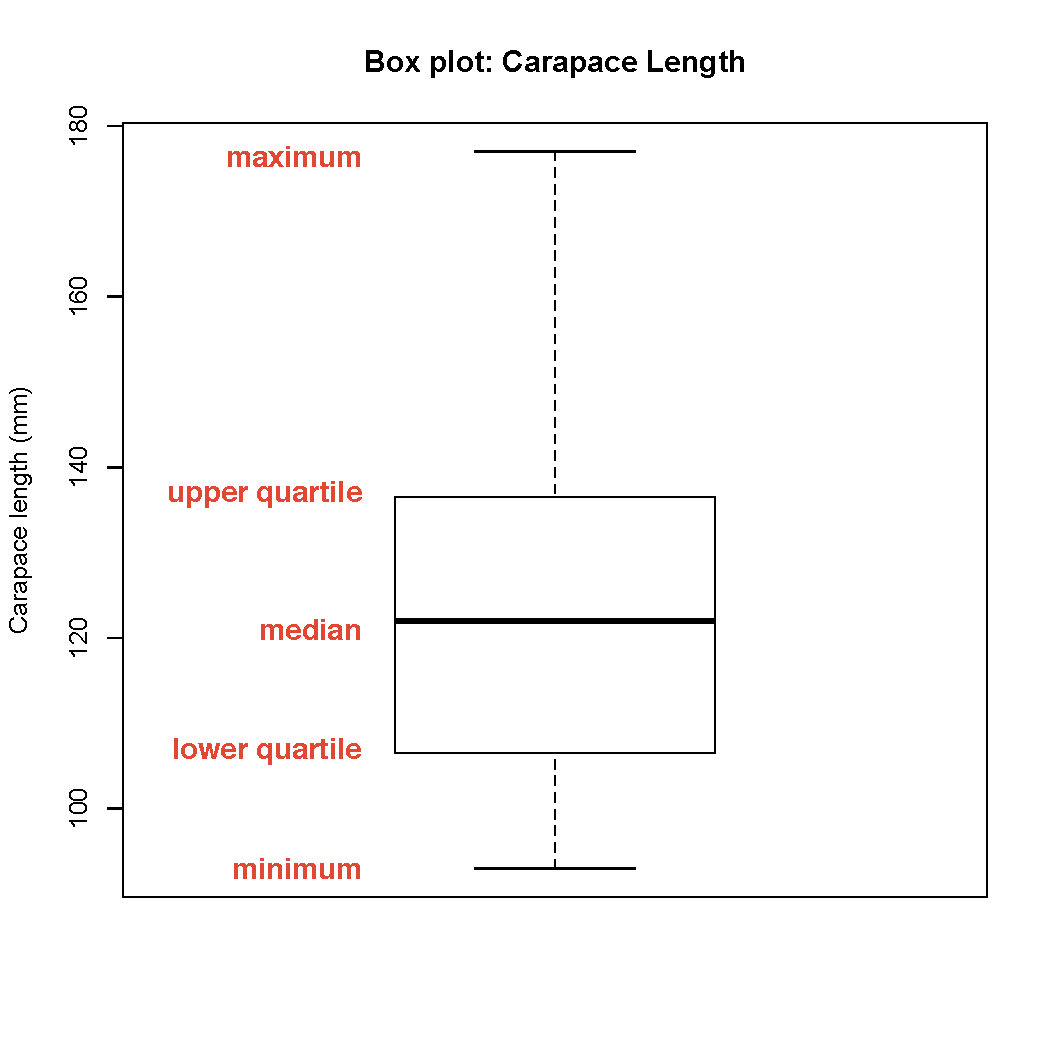
\includegraphics[width=0.5\columnwidth]{./figures/hands-on2/boxplot-labeled.pdf}
\caption{A box plot represents a five number summary of a set of
observations.}
\end{figure}

There are many variants on box plots, particularly with respect to the
`whiskers'. It's always a good idea to be explicit about what a box plot
you've created depicts.

Here's how to create box plots using the standard R functions as well as
the lattice package:

\begin{R}
> boxplot(turtles$length)
> boxplot(turtles$length, col='darkred', horizontal=T) # horizontal version
> title(main = 'Box plot: Carapace Length', ylab = 'Carapace length (mm)')
> bwplot(~length,data=turtles) # using the bwplot function from lattice
\end{R}
Note how we used the \lstinline!title()! function to change the axis
labels and add a plot title.

\paragraph{Historical note}

-- The box plot is one of many inventions of the statistician John W.
Tukey. Tukey made many contributions to the field of statistics and
computer science, particularly in the areas of graphical representations
of data and exploratory data analysis.

\subsection{Bean Plots}

My personal favorite way to depict univariate distributions is called a
`beanplot'. Beanplots combine features of density plots and boxplots and
provide information rich graphical summaries of single variables. The
standard features in a beanplot include the individual observations
(depicted as lines), the density trace estimated from the observations,
the mean of the observations, and in the case of multiple beanplots an
overall mean.

\begin{figure}[htbp]
\centering
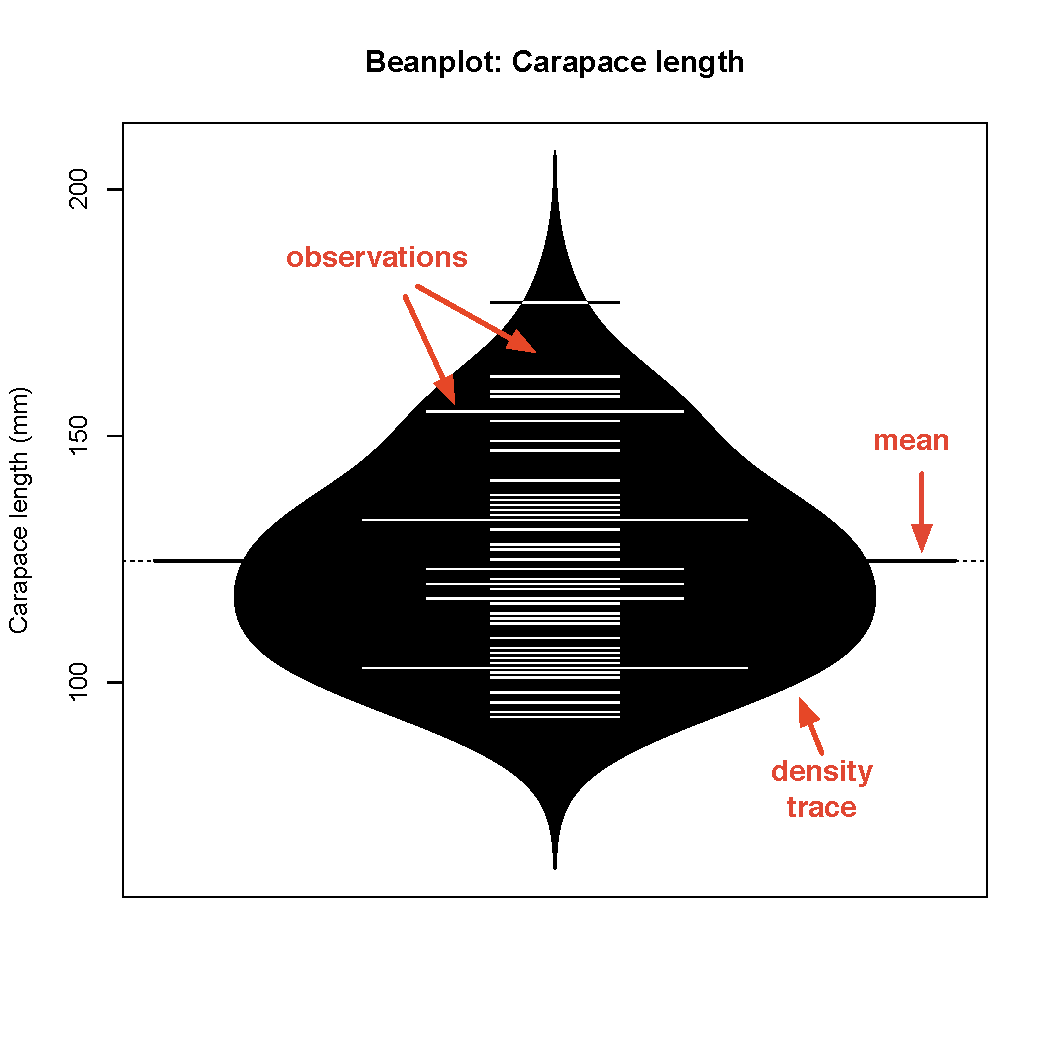
\includegraphics[width=0.5\columnwidth]{./figures/hands-on2/beanplot-labeled.pdf}
\caption{Beanplots combine features of density and box plots.}
\end{figure}

The \lstinline!beanplot! package is not installed by default. To
download it and install it use the R package installer under the
\lstinline!Packages & Data! menu. If this
is the first time you use the package installer you'll have to choose a
CRAN repository from which to download package info (I recommend you
pick one in the US). Once you've done so you can search for `beanplot'
from the Package Installer window. You should also check the 'install
dependencies' check box.

Once the beanplot package has been installed check out the examples to
see some of the capabilities:

\begin{R}
> library(beanplot)
> example(beanplot)
\end{R}

Note the use of the \lstinline!library()! function to make the functions
in the \lstinline!beanplot! library available for use. Here's some
examples of using the \lstinline!beanplot! function with the turtle data
set:

\begin{R}
> beanplot(turtles$length) # note the message about log='y'
> beanplot(turtles$length, log='') # DON'T do the automatic log transform
> beanplot(turtles$length, log='', col=c('white','blue','blue','red'))
\end{R}
In the final version we specified colors for the parts of the beanplot.
See the explanation of the \lstinline!col! argument int he beanplot
function for details.

We can also compare the carapace length variable for male and female
turtles.

\begin{R}
> beanplot(length ~ sex, data = turtles, col=list(c('red'),c('black')),
names = c('females','males'),xlab='Sex', ylab='Caparace length (mm)')
\end{R}
Note the use of the formula notation to compare the carapace length
variable for males and females. There is also a asymmetrical version of
the beanplot which can be used to more directly compare distributions
between two groups. We explore this below. Note too the use of the list
argument to \lstinline!col!, and the use of vectors within the list to
specify the colors for female and male beanplots.

We can also create a beanplot with multiple variables in the same plot
if the variables are measured on the same scale.

\begin{R}
> beanplot(turtles$length, turtles$width, turtles$height, log='',
names=c('length','width','height'), ylab='carapace dimensions (mm)')
\end{R}



\subsection{Demo Plots in R}

To get a sense of some of the graphical power of R try the
\lstinline!demo()! function:
%
\begin{R}
> demo(graphics)
\end{R}


%!TEX root = ./hands-on1.tex

\subsection{Sweave for R}

Sweave documents weave together documentation/discussion and code into a
single document. The pieces of code and documentation are referred to as
`chunks'. R comes with a set of tools that allow you to extract just the
code, or to turn the entire document into a nicely formatted report.

Here's a simple Sweave document to get you started:
%
\begin{noindentcodeblock}[tex]
\documentclass{article}
\begin{document}

This is a very simple Sweave file. It includes only a single code chunk.

<<>>=
z <- rnorm(30, mean=0, sd=1)
summary(z)
@

That code chunk generated a random sample of 30 observations drawn from a normal distribution with mean zero and standard deviation one.

\end{document}  
\end{noindentcodeblock}
%
Type those lines into a text editor and save the document with the name
|sweave1.Rnw|.

Let's break down the various pieces of the document. The first two lines
and the last line represent LaTeX~commands.

\begin{code}{tex}
\documentclass{article}
\begin{document}
    ....
\end{document}
\end{code}
For simple Sweave documents that's all the LaTeX you need to learn.
However, learning a little bit more about the document preparation
system gives you the option of producing very nicely formatted output as
we'll see in a little bit.

The R code is preceeded by the text |<<>>=|. This tells Sweave
that you're starting a code chunk. The |@| symbol after the
code chunk tells Sweave that you're going back to writing documentation
chunks.

If you already have a working installation of LaTeX on your computer you
can now compile this into a nicely formatted document from the R
interpretter. Change the R working directory so that it's in the same
directory where you saved the |sweave1.Rnw| file. The execute
the following commands:
%
\begin{R}
> library(tools)  # makes the texi2dvi function available
> Sweave('sweave1.Rnw') # compiles our Sweave document into 'sweave1.tex'
> texi2dvi("sweave1.tex", pdf = TRUE)
\end{R}
%
These commands will produce two new documents -- |sweave1.tex|
and a PDF document, |sweave1.pdf|. You can open the
|sweave1.tex| file in any text editor and you'll see that it's
just a slightly modified version of the |sweave1.Rnw| file you
created. The PDF file contains the nicely formatted report.

If you got an error message the most likely reason is that R can't find
the path to your LaTeX executable. To check this try:
%
\begin{R}
> texi2dvi('sweave1.tex', pdf=TRUE, quiet=FALSE)
\end{R}
%
If that's the case, you can fix that by typing the following into the R
command line (on OS X):
%
\begin{R}
> Sys.setenv("PATH" = paste(Sys.getenv("PATH"),"/usr/texbin",sep=":"))  
\end{R}
%
Then try executing the |texi2dvi| command again. If that
solved your problem you can make this permanent by adding that line to
your |.Rprofile| (located in |/Users/yourname| on \OSX; if the
file doesn't already exist go ahead and create it). If that doesn't work
please see me for troubleshooting help.

\subsubsection{RStudio makes Sweaving easy!}

RStudio hides some of the complexity of Sweaving documents. Simply
create or open your Sweave document (use the .Rnw extension) in RStudio
and then hit the |Compile PDF| button. If your LaTeX setup is
working, and the document and code are valid, Rstudio will compile
everything behind the scenes and pop up a nice PDF.

\subsubsection{A fancier Sweave document}

Let's get a little bit fancier and show how we can create graphics and
use some LaTeX formatting features to produce a nicer document.

\begin{codeblock}[tex]
\documentclass[letterpaper]{article}
\usepackage[margin=0.75in]{geometry}

\title{My Second Sweave Report}
\author{John Q. Public}

\begin{document}
\maketitle
This is a still a simple Sweave file. However, now it includes several code chunks and several \LaTeX\ specific commands.

\section{Sampling from the random normal distribution}

<<>>=
z <- rnorm(30, mean=0, sd=1)
summary(z)
@

That code chunk generated a random sample of 30 observations drawn from a normal distribution with mean zero ($\mu = 0$) and standard deviation one ($\sigma = 1$).

\section{Generating figures}

We can also automatically imbed graphics in our report. For example, the following will generate a histogram.

% this tells Sweave to set the graphics 
% to be half the width of the text
\setkeys{Gin}{width=0.5\textwidth} 
<<fig=TRUE>>=
hist(z)
@

\end{document}    
\end{codeblock}
%
Notice how we put an argument, |fig=TRUE| within the second
code chunk delimiter. This will tell Sweave to automatically imbed a
figure with the histogram graphic we created into our report. Save this
as |sweave2.Rnw| and repeat the above steps to compile it into
a PDF report.

For a full overview of Sweave's capabilities see the documentation for
Sweave availabe at
\url{http://www.stat.uni-muenchen.de/~leisch/Sweave/}.

\subsection{Pweave for literate programming in Python}

Pweave uses almost exactly the same syntax as Sweave to delimit code and
document chunks. Here's a simple Pweave document.

\begin{codeblock}[tex]
\documentclass[letterpaper]{article}
\usepackage[margin=0.75in]{geometry}
\usepackage{graphicx} % unlike Sweave, Pweave doesn't
                      % pull this in automatically

\title{My First Pweave Report}
\author{John Q. Public}

\begin{document}
\maketitle
This is a still a simple Pweave file. As in our Sweave example,
there are several code chunks and we've included a figure.

\section{Sampling from the random normal distribution}

<<>>=
from numpy import random
z = random.normal(loc=0, scale=1, size=30)
@

That code chunk generated a random sample of 30 
observations drawn from a normal distribution with mean 
zero ($\mu = 0$) and standard deviation one ($\sigma = 1$).

\section{Generating figures}

We can also automatically imbed graphics in our 
report. For example, the following will generate 
a histogram.

% this tells Sweave to set the graphics 
% to be half the width of the text
\setkeys{Gin}{width=0.5\textwidth} 
<<fig=True>>=
import pylab
pylab.hist(z)
@

\end{document}
\end{codeblock}
%
Note that the second code chunk, we wrote |fig=True| in the
Pweave document, whereas we wrote |fig=TRUE| for the Sweave
document. This minor difference reflects the different syntax for
boolean values in R and Python.

Save that code in a text file called |pweave1.Pnw| and from
the bash shell (\emph{not} in the Python interpretter) type the
following command:
%
\begin{bash}
Pweave -f "tex" pweave1.Pnw
\end{bash}
%
The option |-f "tex"| tells Pweave to output a file (Note:
from the Windows command prompt you must use double quotes around
``tex'', on Unix-based systems either single our double quotes work
fine). Assuming you got no error messages, you can then compile this to
PDF using the following command:
%
\begin{bash}
pdflatex pweave1.tex
\end{bash}



\chapter{Bivariate Data}

%!TEX root = ./workbook-2011.tex

\section{Vector Operations in R}

As you saw last week R vectors support basic arithmetic operations that
correspond to the same operations on geometric vectors. For example:
%
\begin{R}
> x <- 1:15
> y <- 10:24
> x
 [1]  1  2  3  4  5  6  7  8  9 10 11 12 13 14 15
> y
 [1] 10 11 12 13 14 15 16 17 18 19 20 21 22 23 24

> x + y             # vector addition
 [1] 11 13 15 17 19 21 23 25 27 29 31 33 35 37 39
> x - y             # vector subtraction
 [1] -9 -9 -9 -9 -9 -9 -9 -9 -9 -9 -9 -9 -9 -9 -9
> x * 3             # multiplication by a scalar
 [1]  3  6  9 12 15 18 21 24 27 30 33 36 39 42 45
\end{R}
%
R also has an operator for the dot product, denoted \lstinline!%*%!.
This operator also designates matrix multiplication, which we will
discuss next week. By default this operator returns an object of the R
matrix class. If you want a scalar (or the R equivalent of a scalar,
i.e.~a vector of length 1) you need to use the \lstinline!drop()!
function.

\begin{R}
> z <- x %*% x
> class(z)      # note use of class() function
[1] "matrix"
> z
     [,1]
[1,] 1240
> drop(z)
[1] 1240
\end{R}

In lecture we saw that many useful geometric properties of vectors could be expressed in the form of dot products. Let's start with some two-dimensional vectors where the geometry is  easy to visualize:

\begin{R}
> a <- c(1, 0) # the point (1,0)
> b <- c(0, 1) # the point (0,1)
\end{R}
%
Now let's draw our vectors:
%
\begin{R}
# create empty plot w/specified x- and y- limits
# the 'asp=1' argument maintains the scaling of the x- and y-axes
# so that units are equivalent for both axes (i.e. squares remain squares)
> plot(c(-2,2),c(-1,2),type='n', asp=1)

# draw an arrow from origin (0,0) to x,y coordinates of vector "a"
# the length argument changes the size of the arrowhead
# use the R help to read more about the arrows function
> arrows(0, 0, a[1], a[2], length=0.1)

# and now for the vector "b"
> arrows(0, 0, b[1], b[2], length=0.1)
\end{R}
%
You should now have a figure that looks like the one below:
\begin{figure}[htbp]
\centering
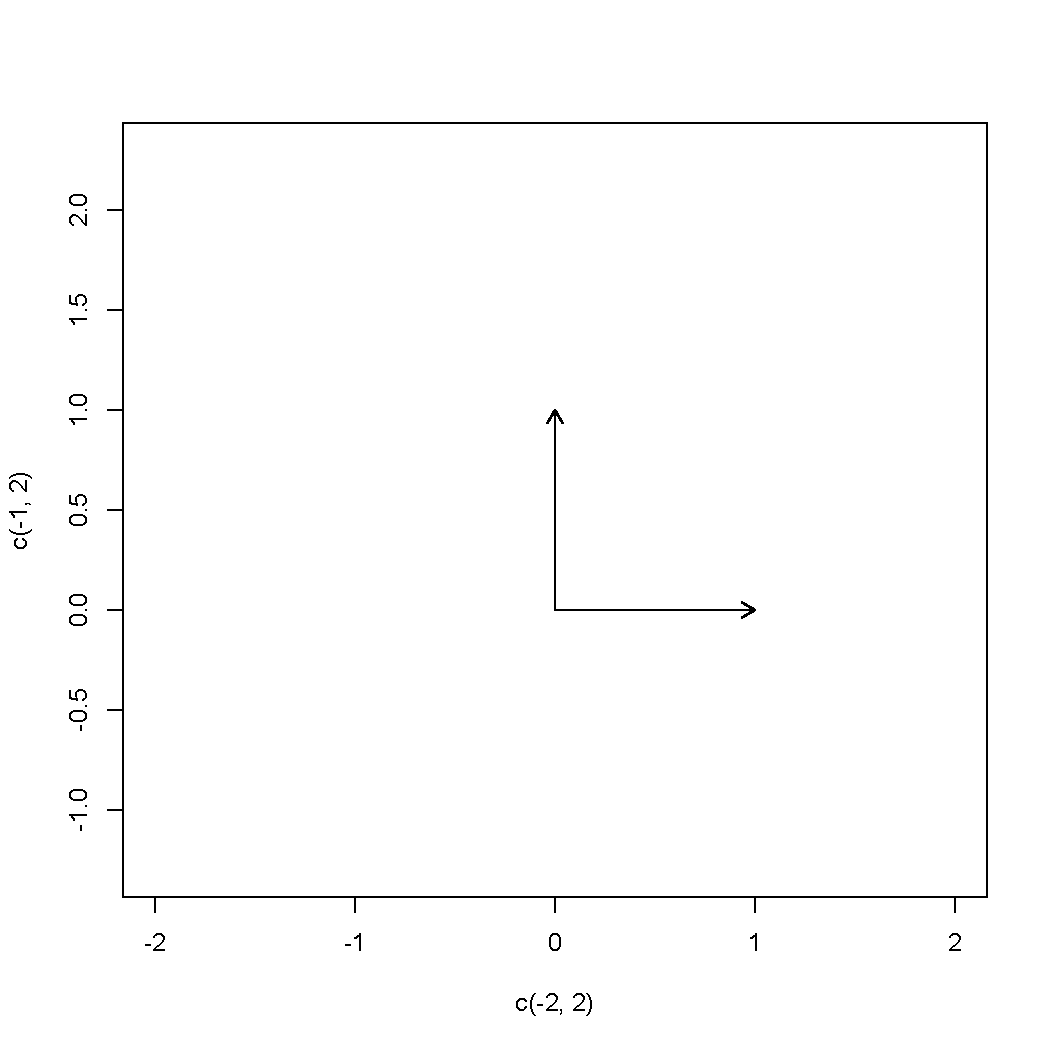
\includegraphics[width=0.33\columnwidth]{./figures/hands-on2/rightangle.pdf}
\caption{A simple vector figure.}
\end{figure}
%
Let's see what the dot product can tell us about these vectors. First recall that we can calculate the length of a vector as the square-root of the dot product of the vector with itself ($\vert\vec{a}\vert^2  =  \vec{a} \cdot \vec{a}$)
\begin{R}
> len.a <- drop(sqrt(a %*% a))
> len.a
[1] 1
> len.b <- drop(sqrt(b %*% b))
\end{R}
%
How about the angle between $a$ and $b$?
\begin{R}
> dot.ab <- a %*% b
> dot.ab
     [,1]
[1,]    0
> cos.ab <- (a %*% b)/(len.a * len.b)
> cos.ab
     [,1]
[1,]    0
\end{R}
A key point to remember dot product of two vectors is zero if, and only if, they are orthogonal to each other (regardless of their dimension).




%!TEX root = ./workbook-2011.tex

\section{Writing Functions in R}

So far we've been mostly using R's built in functions. However the power of a
true programming language is the ability to write your own functions.

The general form of an R function is as follows:

\begin{R}
funcname <- function(arg1, arg2) {
 # one or more expressions
 # last expression is the object returned
 # or you can explicitly return an object
}
\end{R}
To make this concrete, here's an example where we define a function in
the interpreter and then put it to use:
%
\begin{R}
> myfunc <- function(x,y){
+ # don't type the '+' symbols, these show continuation lines
+   x^2 + y^2
+ }

> a <- 1:5
> b <- 6:10
> a
[1] 1 2 3 4 5
> b
[1]  6  7  8  9 10
> myfunc(a,b)
[1]  37  53  73  97 125
> myfunc
function(x,y){
  x^2 + y^2
}
\end{R}
%
If you type a function name without parentheses R shows you the
function's definition. This works for built-in functions as well
(thought sometimes these functions are defined in C code in which case R
will tell you that the function is a `.Primitive').

\subsection{Putting R functions in Scripts}

When you define a function at the interactive prompt and then close the
interpreter your function definition will be lost. The simple way around
this is to define your R functions in a script that you can than access
at any time.

Choose \lstinline!File > New Script! (or \lstinline!File > New Document! in OS
X) in the R GUI . This
will bring up a blank editor window. Enter your function into the editor
and save the source file in your R working directory with a name like
\lstinline!vecgeom.R!.

\begin{R}
# functions defined in vecgeom.R

veclength <- function(x) {
  # Given a numeric vector, returns length of that vector
  sqrt(drop(x %*% x))
}

unitvector <- function(x) {
  # Return a unit vector in the same direction as x
  x/veclength(x)
}

vec.cos <- function(x,y) {
  # Calculate the cos of the angle between vectors x and y
  len.x <- veclength(x)
  len.y <- veclength(y)
  return( (x %*% y)/(len.x * len.y) )
}

\end{R}
There are two functions defined above, one of which calls the other.
Both take single vector arguments. At this point there is no error
checking to insure that the argument is reasonable but R's built in
error handling will do just fine for now.

Once your functions are in a script file you can make them accesible by
using the \lstinline!source()! function (See also the
\lstinline!File > Source R code...! menu item in the R GUI):
%
\begin{R}
> source("vecgeom.R")
> x <- c(1,0.4)
> veclength(x)
[1] 1.077033
> ux <- unitvector(x)
> ux
[1] 0.9284767 0.3713907
> veclength(ux)
[1] 1
\end{R}

Let's also add the following function to |vecgeom.R| to aid in visualizaing 2D vectors:
%
\begin{R}
draw.vectors <- function(a, b, colors=c('red', 'blue'), clear.plot=TRUE){

    # figure out the limits such that the origin and the vector
    # end points are all included in the plot
    xhi <- max(0, a[1], b[1])
    xlo <- min(0, a[1], b[1])
    yhi <- max(0, a[2], b[2])
    ylo <- min(0, a[2], b[2])

    xlims <- c(xlo, xhi)*1.10 # give a little breathing space around vectors
    ylims <- c(ylo, yhi)*1.10

    if (clear.plot){
        plot(xlims, ylims, type='n', asp=1, xlab="x-coord", ylab="y-coord")
    }
    arrows(0, 0, a[1], a[2], length=0.1, col=colors[1])
    arrows(0, 0, b[1], b[2], length=0.1, col=colors[2])
}
\end{R}
%
You can use this new function as follows:
\begin{R}
# you need to source the file everytime you change it
> source("/Users/pmagwene/Downloads/vecgeom.R")
> x <- c(1,0.4)
> y <- c(0.2, 0.8)
> draw.vectors(x,y)  # draw the original vectors
\end{R}
%
The resulting figure should resemble the one below.
%
\begin{figure}[htbp]
\centering
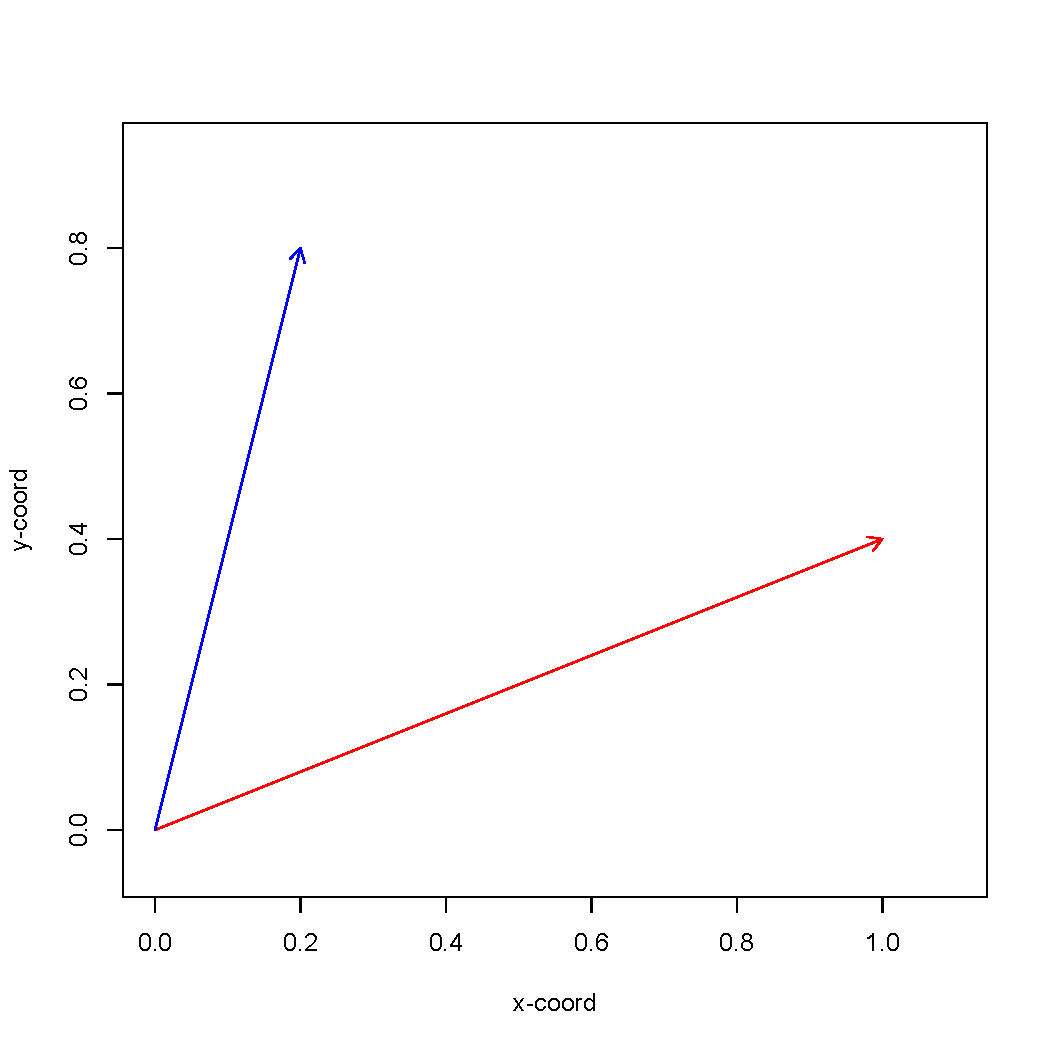
\includegraphics[width=0.33\columnwidth]{./figures/hands-on2/vecfig2.pdf}
\caption{Another vector figure.}
\end{figure}

Notice that we included a |clear.plot| argument in our |draw.vectors| function. I included this so we could add additional vectors to our plot, without overwriting the old vectors, as demonstrated below:
\begin{R}
# draw the unit vectors that point in the same directors as the original vectors
> ux <- unitvector(x)
> uy <- unitvector(y)
> draw.vectors(ux, uy, colors=c('black', 'green'), clear.plot=F)
\end{R}

\begin{assignment}
Write a function in R that takes two vectors, $\vec{x}$ and $\vec{y}$, and returns a list containing the projection of $\vec{y}$ on $\vec{x}$ and the component of $\vec{y}$ in $\vec{x}$:

\lstDeleteShortInline|

\[P_{\vec{x}}(\vec{y}) = \left(\frac{\vec{x} \cdot \vec{y}}{|\vec{x}|}\right) \frac{\vec{x}}{|\vec{x}|}\]
and
\[C_{\vec{x}}(\vec{y}) = \frac{\vec{x} \cdot \vec{y}}{|\vec{x}|}\]

\lstMakeShortInline|

\end{assignment}



%%!TEX root = ./workbook-2011.tex

\section{Basic statistical functions in R}

\subsection{Dealing with Data Subsets in R}

Manipulating or analyzing subsets of data is one of the most common
tasks in R. The \lstinline!subset()! function comes in handy for such
operations. Consider the data set \lstinline!turtles.txt!:
%
\begin{R}
> turtles <- read.table('turtles.txt', header=T)
> turtles
   sex length width height
1    f     98    81     38
2    f    103    84     38
3    f    103    86     42
  # output truncated
> names(turtles)
[1] "sex"    "length" "width"  "height"
> # Now we'll apply the subset() function
> turt.sub <- subset(turtles, select = -sex)
> names(turt.sub)
[1] "length" "width"  "height"
> turt.sub
   length width height
1      98    81     38
2     103    84     38
3     103    86     42
  # output truncated
\end{R}
%
In the example above we create a subset of the original data set by
excluding the variable indicating the sex of each individual using the
argument \lstinline!select = -sex!. We can also explicit include only
certain variables, like this:
%
\begin{R}
> turt.sub2 <- subset(turtles, select=c(height,width))
> turt.sub2
   height width
1      38    81
2      38    84
3      42    86
  # output truncated    
\end{R}
%
\lstinline!subset()! allows you to do more than just select variables to
include. You can use the second positional argument to specify matching
criteria. For example:
%
\begin{R}
# gives only female turtles, all variables except sex
> female.turts <- subset(turtles, sex == "f", select = -sex)
> dim(female.turts)
[1] 24  3
# same for male turtles
> male.turts <- subset(turtles, sex == "m", select = -sex)
> dim(male.turts)
[1] 24  3
# gives only females with length > 125, all variables
> big.females <- subset(turtles, sex == "f" & length > 125)    
\end{R}

The \lstinline!subset! function is especially useful when combined with
the function \lstinline!sapply()! which allows you to apply a function
of interest to each variable. For example:
%
\begin{R}
> min(turtles)
Error in Summary.data.frame(..., na.rm = na.rm) : 
        only defined on a data frame with all numeric or complex variables
> min(turt.sub)  # unexpected result
[1] 35
> sapply(turt.sub, min) # here's what we were shooting for
length  width height 
    93     74     35
> sapply(female.turts, min) # for females
length  width height 
    98     81     38 
> sapply(male.turts, min) # for males
length  width height 
    93     74     35      
\end{R}
%
Notice how the \lstinline!min()! function chokes on the complete data
set because the function is not defined for factor variables. In the
second example \lstinline!min(turt.sub)! returns a valid result, but
also not exactly what we wanted. In this case it looked for the minimum
value across all the objects passed to it. In the third case we use the
\lstinline!sapply()! function and get the minimum on a
variable-by-variable basis. Please take a moment to look at the
documentation for the \lstinline!sapply()! function and cook up some
examples of your own.

\paragraph{Anderson's (Fisher's) iris data set}

Anderson's (or Fisher's) iris data set consists of four morphometric
measurements for specimens from three different iris species. Use the R
help to read about the iris data set (\lstinline!?iris!). We'll be using
this data set repeatedly in future weeks so familiarize yourself with
it.

\smallskip
\begin{assignment}
Calculate a summary table as well as correlation
and covariance matrices for each of the species in the iris data set.
Use \lstinline!help.search()! and \lstinline!apropos()! to lookup any
necessary function names.
\end{assignment}


\subsection{Exploring Univariate Distributions in R}

\subsubsection{Histograms}

One of the most common ways to examine a the distribution of
observations for a single variable is to use a histogram. The
\lstinline!hist()! function creates simple histograms in R.

\begin{R}
> hist(turtles$length) # create histogram with fxn defaults
> ?hist # check out the documentation on hist
\end{R}
Note that by default the \lstinline!hist()! function plots the
frequencies in each bin. If you want the probability densities instead
set the argument \lstinline!freq=FALSE!.
%
\begin{R}
> hist(turtles$length,freq=F) # y-axis gives probability density
\end{R}
Here's some other ways to fine tune a histogram in R.

\begin{R}
> hist(turtles$length, breaks=12) # use 12 bins
> mybreaks = seq(85,185,8)
> hist(turtles$length, breaks=mybreaks) # specify bin boundaries   
> hist(turtles$length, breaks=mybreaks, col='red') # fill the bins with red  
\end{R}

\subsubsection{Density Plots}

One of the problems with histograms is that they can be very sensitive
to the size of the bins and the break points used. This is due to the
discretization inherent in a histogram. A `density plot' or `density
trace' is a continuous estimate of a probability distribution from a set
of observations. Because it is continuous it doesn't suffer from the
same sensitivity to bin sizes and break points. One way to think about a
density plot is as the histogram you'd get if you averaged many
individual histograms each with slightly different breakpoints.
%
\begin{R}
> d <- density(turtles$length)
> plot(d)    
\end{R}
%
A density plot isn't entirely parameter free -- the parameter you should
be most aware of is the `smoothing bandwidth'.

\begin{R}
> d <- density(turtles$length) # let R pick the bandwidth
> plot(d,ylim=c(0,0.020)) # gives ourselves some extra headroom on y-axis
> d2 <- density(turtles$length, bw=5) # specify bandwidth
> lines(d2, col='red') # use lines to draw over previous plot
\end{R}
The bandwidth determines the standard deviation of the `kernel' that is
used to calculate the density plot. There are a number of different
types of kernels you can use; a Gaussian kernel is the R default and is
the most common choice. See the documentation for more info.

The \lstinline!lattice! package is an R library that makes it easier to
create graphics that show conditional distributions. Here's how to
create a simple density plot using the \lstinline!lattice! package.

\begin{R}
> library(lattice)
> densityplot(turtles$length) # densityplot defined in lattice
\end{R}
Notice how by default the \lstinline!lattice! package also drew points
representing the observations along the x-axis. These points have been
`jittered' meaning they've been randomly shifted by a small amount so
that overlapping points don't completely hide each other. We could have
produced a similar plot, without the lattice package, as so:

\begin{R}
> d <- density(turtles$length)
> plot(d)
> nobs <- length(turtles$length)
> points(jitter(turtles$length), rep(0,nobs)) 
\end{R}
Notice that in our version we only jittered the points along the x-axis.
You can also combine a histogram and density trace, like so:

\begin{R}
> hist(turtles$length, 10, xlab='Carapace Length (mm)',freq=F)
> d <- density(turtles$length)
> lines(d, col='red', lwd=2) # red lines, with pixel width 2    
\end{R}
Notice the use of the \lstinline!freq=F! argument to scale the histogram
bars in terms of probability density.

Finally, let's some of the features of \lstinline!lattice! to produce
density plots for the `length' variable of the turtle data set,
conditional on sex of the specimen.

\begin{R}
> densityplot(~length | sex, data = turtles)    
\end{R}
There are a number of new concepts here. The first is that we used what
is called a `formula' to specify what to plot. In this case the formula
can be read as `length conditional on sex'. We'll be using formulas in
several other contexts and we discuss them at greater length below. The
\lstinline!data! argument allows us to specify a data frame or list so
that we don't always have to write arguments like
\lstinline!turtles$length! or \lstinline!turtles$sex! which can get a
bit tedious.

\subsubsection{Box Plots}

Another common tool for depicting a univariate distribution is a `box
plot' (sometimes called a box-and-whisker plot). A standard box plot
depicts five useful features of a set of observations: the median
(center most line), the upper and lower quartiles (top and bottom of the
box), and the minimum and maximum observations (ends of the whiskers).

\begin{figure}[htbp]
\centering
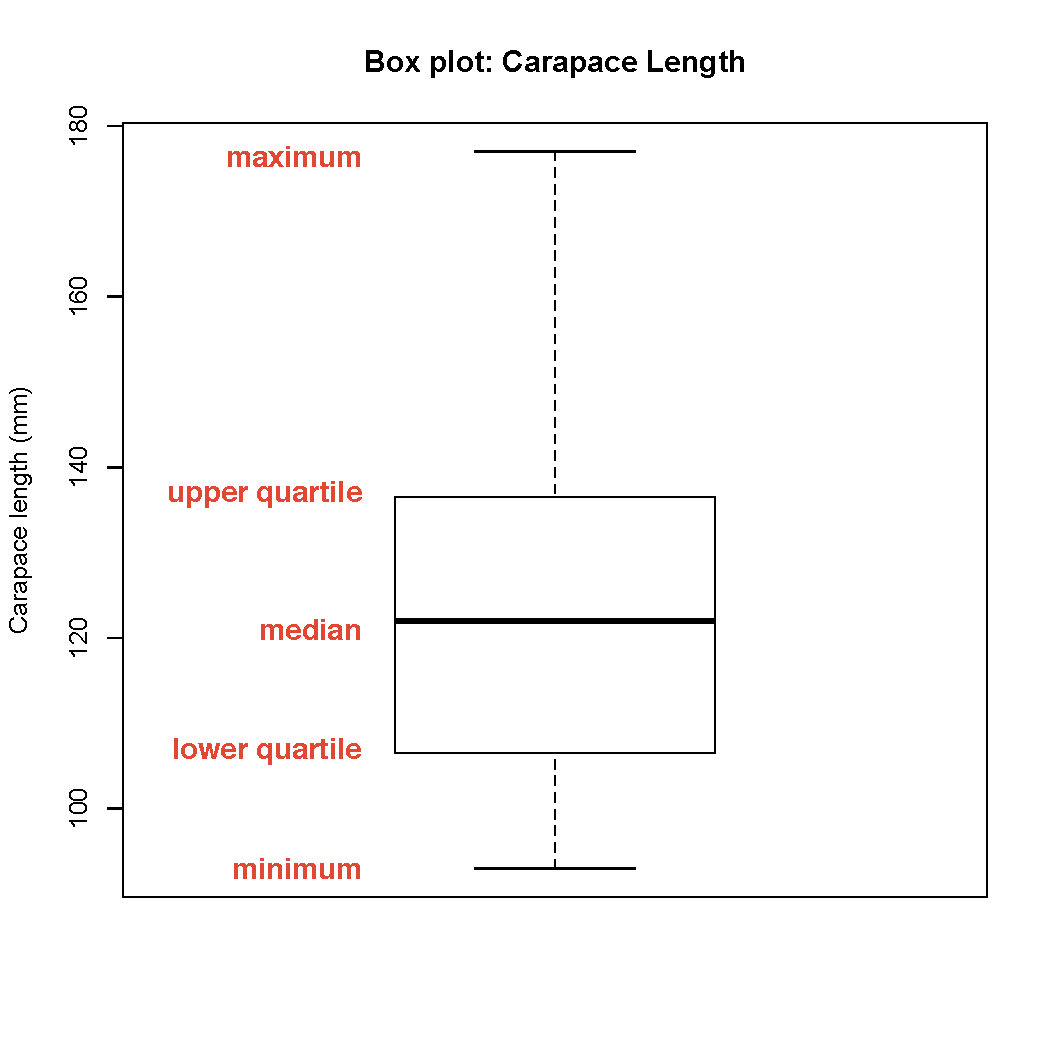
\includegraphics[width=0.5\columnwidth]{./figures/hands-on2/boxplot-labeled.pdf}
\caption{A box plot represents a five number summary of a set of
observations.}
\end{figure}

There are many variants on box plots, particularly with respect to the
`whiskers'. It's always a good idea to be explicit about what a box plot
you've created depicts.

Here's how to create box plots using the standard R functions as well as
the lattice package:

\begin{R}
> boxplot(turtles$length)
> boxplot(turtles$length, col='darkred', horizontal=T) # horizontal version 
> title(main = 'Box plot: Carapace Length', ylab = 'Carapace length (mm)')
> bwplot(~length,data=turtles) # using the bwplot function from lattice
\end{R}
Note how we used the \lstinline!title()! function to change the axis
labels and add a plot title.

\paragraph{Historical note}

-- The box plot is one of many inventions of the statistician John W.
Tukey. Tukey made many contributions to the field of statistics and
computer science, particularly in the areas of graphical representations
of data and exploratory data analysis.

\subsubsection{Bean Plots}

My personal favorite way to depict univariate distributions is called a
`beanplot'. Beanplots combine features of density plots and boxplots and
provide information rich graphical summaries of single variables. The
standard features in a beanplot include the individual observations
(depicted as lines), the density trace estimated from the observations,
the mean of the observations, and in the case of multiple beanplots an
overall mean.

\begin{figure}[htbp]
\centering
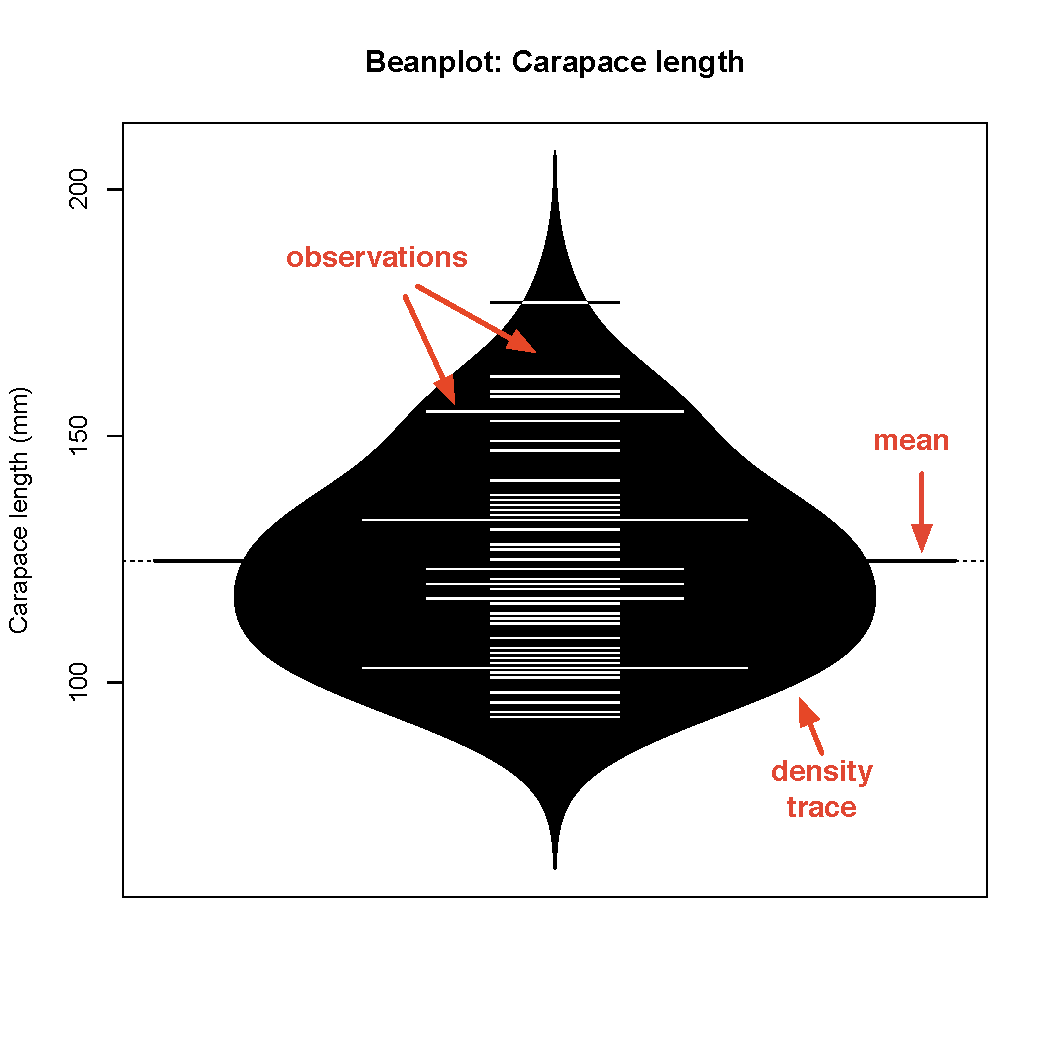
\includegraphics[width=0.5\columnwidth]{./figures/hands-on2/beanplot-labeled.pdf}
\caption{Beanplots combine features of density and box plots.}
\end{figure}

The \lstinline!beanplot! package is not installed by default. To
download it and install it use the R package installer under the
\lstinline!Packages & Data! menu (standard R GUI) or in
\lstinline!Tools > Install Packages...! in RStudio (see also the
\lstinline!Packages! tab in the lower-right window in RStudio). If this
is the first time you use the package installer you'll have to choose a
CRAN repository from which to download package info (I recommend you
pick one in the US). Once you've done so you can search for `beanplot'
from the Package Installer window. You should also check the 'install
dependencies' check box.

Once the beanplot package has been installed check out the examples to
see some of the capabilities:

\begin{R}
> library(beanplot) 
> example(beanplot)    
\end{R}
If you ran the examples in RStudio, use the \lstinline!Clear All! option
in the \lstinline!Plots! tab after running the examples in order to
reset parameters that the examples changed.

Note the use of the \lstinline!library()! function to make the functions
in the \lstinline!beanplot! library available for use. Here's some
examples of using the \lstinline!beanplot! function with the turtle data
set:

\begin{R}
> beanplot(turtles$length) # note the message about log='y'
> beanplot(turtles$length, log='') # DON'T do the automatic log transform
> beanplot(turtles$length, log='', col=c('white','blue','blue','red'))
\end{R}
In the final version we specified colors for the parts of the beanplot.
See the explanation of the \lstinline!col! argument int he beanplot
function for details.

We can also compare the carapace length variable for male and female
turtles.

\begin{R}
> beanplot(length ~ sex, data = turtles, col=list(c('red'),c('black')),
names = c('females','males'),xlab='Sex', ylab='Caparace length (mm)')
\end{R}
Note the use of the formula notation to compare the carapace length
variable for males and females. There is also a asymmetrical version of
the beanplot which can be used to more directly compare distributions
between two groups. We explore this below. Note too the use of the list
argument to \lstinline!col!, and the use of vectors within the list to
specify the colors for female and male beanplots.

We can also create a beanplot with multiple variables in the same plot
if the variables are measured on the same scale.

\begin{R}
> beanplot(turtles$length, turtles$width, turtles$height, log='',
names=c('length','width','height'), ylab='carapace dimensions (mm)') 
\end{R}


\subsection{Simple t-tests in R}

Student's t-tests can be carried out in R using the function
\lstinline!t.test()!. The \lstinline!t.test()! function can perform one
and two-sample t-tests (i.e.~comparing a sample of interest against a
hypothesized mean, or comparing the means of two samples). The
\lstinline!t.test()! function also supports a `formula' interface for
two-sample t-tests similar to the \lstinline!lm(!) function.

\begin{R}
> t.test(width ~ sex, data=turtles)

        Welch Two Sample t-test

data:  width by sex 
t = 4.7015, df = 35.355, p-value = 3.862e-05
alternative hypothesis: true difference in means is not equal to 0 
95 percent confidence interval:
  8.122699 20.460634 
sample estimates:
mean in group f mean in group m 
      102.58333        88.29167 
\end{R}
The asymmetric version of the boxplot is very useful for comparing
distributions of the same variable between two groups. To generate such
plots use the argument \lstinline!side='both'! as an argument to
\lstinline!beanplot!.

\begin{R}
> beanplot(width ~ sex, data = turtles, side='both', col=list(c('red'),c('black')))  
\end{R}
As you can see this splits the beanplot in half for each group and puts
them back to back to facilitate comparison. The difference in the mean
of the two groups is visually obvious from the beanplot.

\begin{assignment}
\begin{enumerate}[a)]
\item
  Prepare beanplots showing samples grouped by \lstinline!Species! for
  each of the quantitative variables in the iris data set. Label the x-
  and y-axes of your boxplots and give each plot a title. \textbf{Tip}: since there are three species, you can't use the \lstinline!side='both'! argument, and you'll need to extend the \lstinline!col=list! argument to add a third color.

\item Carry out two-sample t-tests contrasting \lstinline!versicolor! and
  \lstinline!virginica! for each of the four morphometric variables in
  the iris data set. \textbf{Tip}: use the \lstinline!subset()! function to create a subset of the iris data containing just these two species.

\item Write a brief paragraph interpreting the results of the t-tests you
  conducted.
\end{enumerate}
\end{assignment}

\subsection{Exploring Bivariate Distributions in R}

\subsubsection{Scatterplots}

When dealing with pairs of continuous variables a scatter plot is the
obvious choice. The standard \lstinline!plot! function can be used:

\begin{R}
> plot(turtles$length, turtles$width)
> plot(turtles$length ~ turtles$width)    
\end{R}
Did you notice what is different between the two versions above? You can
also use the \lstinline!data! argument with plot, like so:

\begin{R}
> plot(length ~ width, data=turtles)
\end{R}
The \lstinline!xyplot()! function from the \lstinline!lattice! package
does pretty much the same thing:
%
\begin{R}
> xyplot(length ~ width, data = turtles)
\end{R}


\subsubsection{Regression in R}

R has very flexible built in functions for fitting linear models.
Bivariate regression is the simplest case of a linear model.

\begin{R}
> turtles <- read.table('turtles.txt',header=T)
> names(turtles)
[1] "sex"    "length" "width"  "height"
> regr <- lm(turtles$width ~ turtles$length)
> class(regr)
[1] "lm"
> names(regr)
 [1] "coefficients"  "residuals"     "effects"       "rank"          "fitted.values"
 [6] "assign"        "qr"            "df.residual"   "xlevels"       "call"         
[11] "terms"         "model"   
> summary(regr)

Call:
lm(formula = turtles$width ~ turtles$length)

Residuals:
     Min       1Q   Median       3Q      Max 
-5.57976 -1.66578 -0.04471  1.73752  5.97104 

Coefficients:
               Estimate Std. Error t value Pr(>|t|)    
(Intercept)     19.9434     2.3877   8.353 8.99e-11 ***
turtles$length   0.6055     0.0189  32.033  < 2e-16 ***
---
Signif. codes:  0 '***' 0.001 '**' 0.01 '*' 0.05 '.' 0.1 ' ' 1 

Residual standard error: 2.654 on 46 degrees of freedom
Multiple R-Squared: 0.9571,     Adjusted R-squared: 0.9562 
F-statistic:  1026 on 1 and 46 DF,  p-value: < 2.2e-16 

> plot(turtles$width ~ turtles$length)  # scatter plot with turtles$length on x axis
> abline(regr)  # plot the regression line
\end{R}
Note the use of the function \lstinline!abline()! to plot the regression
line. Calling \lstinline!plot()! with an object of class \lstinline!lm!
shows a series of diagnostic plots. Try this.

\begin{assignment}
Write your own regression function (i.e.~your
code shouldn't refer to the built in regression functions) for mean
centered vectors in R. The function will take as it's input two vectors,
$\vec{x}$ and $\vec{y}$. The function should return:

\begin{enumerate}[1.]
\item
  a list containing the mean-centered versions of these vectors
\item
  the regression coefficient $b$ in the mean centered regression
  equation $\vec{\widehat{y}} = b\vec{x}$
\item
  the coefficient of determination, $R^2$
\end{enumerate}
Demonstrate your regression function by using it to carry out
regressions of Sepal.Length on Sepal.Width separately for the `setosa'
and `virginica' specimens from the iris data set (again,
\lstinline!subset()! is your friend). Include plots in which you use the
\lstinline!plot()! and \lstinline!abline()! functions to illustrate your
calculated regression line.

\end{assignment}




\chapter{Matrices and matrix operations in R}


\section{Matrices in R}

In R matrices are two-dimensional collections of elements all of which
have the same mode or type. This is different than a data frame in which
the columns of the frame can hold elements of different type (but all of
the same length), or from a list which can hold objects of arbitrary
type and length. Matrices are more efficient for carrying out most
numerical operations, so if you're working with a very large data set
that is amenable to representation by a matrix you should consider using
this data structure.

\subsection{Creating matrices in R}

There are a number of different ways to create matrices in R. For
creating small matrices at the command line you can use the
\lstinline!matrix()! function.

\begin{R}
> X <- matrix(1:5)
> X
      [,1]
 [1,]    1
 [2,]    2
 [3,]    3
 [4,]    4
 [5,]    5
> X <- matrix(1:12, nrow=4)
> X
     [,1] [,2] [,3]
[1,]    1    5    9
[2,]    2    6   10
[3,]    3    7   11
[4,]    4    8   12
> dim(X) # give the shape of the matrix 
[1] 4 3
\end{R}
\lstinline!matrix()! takes a data vector as input and the shape of the
matrix to be created is specified by using the \lstinline!nrow! and
\lstinline!ncol! arguments (if the number of elements in the input data
vector is less than |nrows| $\times$ |ncols| the
elements will be 'recycled' as discussed in previous lectures). Without
any shape arguments the \lstinline!matrix()! function will create a
column vector as shown above. By default the \lstinline!matrix()!
function fills in the matrix in a column-wise fashion. To fill in the
matrix in a row-wise fashion use the argument \lstinline!byrow=T!.

If you have a pre-existing data set in a list or data frame you can use
the \lstinline!as.matrix()! function to convert it to a matrix.

\begin{R}
> turtles <- read.table('turtles.txt', header=T)
> tmtx <- as.matrix(turtles) 
> tmtx   # note how the elements were all converted to character 
   sex length width height
1  "f" " 98"  " 81" "38"  
2  "f" "103"  " 84" "38"  
3  "f" "103"  " 86" "42"  
4  "f" "105"  " 86" "40"  
 ... output truncated ...
> tsub <- subset(turtles, select=-sex)
> tmtx <- as.matrix(tsub)
> tmtx    # this is probably more along the lines of what you want
   length width height
1      98    81     38
2     103    84     38
3     103    86     42
4     105    86     40
 ... output truncated ...
\end{R}
You can use the various indexing operations to get particular rows,
columns, or elements. Here are some examples:

\begin{R}
> X <- matrix(1:12, nrow=4)
> X
     [,1] [,2] [,3]
[1,]    1    5    9
[2,]    2    6   10
[3,]    3    7   11
[4,]    4    8   12
> X[1,] # get the first row
[1] 1 5 9
> X[,1] # get the first column
[1] 1 2 3 4
> X[1:2,] # get the first two rows
     [,1] [,2] [,3]
[1,]    1    5    9
[2,]    2    6   10
> X[,2:3] # get the second and third columns
     [,1] [,2]
[1,]    5    9
[2,]    6   10
[3,]    7   11
[4,]    8   12
> Y <- matrix(1:12, byrow=T, nrow=4)
> Y
     [,1] [,2] [,3]
[1,]    1    2    3
[2,]    4    5    6
[3,]    7    8    9
[4,]   10   11   12
> Y[4] # see explanation below
[1] 10 
> Y[5]
[1] 2
> dim(Y) <- c(2,6)
> Y
     [,1] [,2] [,3] [,4] [,5] [,6]
[1,]    1    7    2    8    3    9
[2,]    4   10    5   11    6   12
> Y[5]
[1] 2
\end{R}
The example above where we create a matrix \lstinline!Y! is meant to
show that matrices are stored internally in a column wise fashion (think
of the columns stacked one atop the other), regardless of whether we use
the \lstinline!byrow=T! argument. Therefore using single indices returns
the elements with respect to this arrangement. Note also the use of
assignment operator in conjuction with the \lstinline!dim()! function to
reshape the matrix. Despite the reshaping, the internal representation
in memory hasn't changed so \lstinline!Y[5]! still gives the same
element.

You can use the \lstinline!diag()! function to get the diagonal of a
matrix or to create a diagonal matrix as show below:

\begin{R}
> Z <- matrix(rnorm(16), ncol=4)
> Z
           [,1]       [,2]         [,3]        [,4]
[1,] -1.7666373  2.1353032 -0.903786375 -0.70527447
[2,] -0.9129580  1.1873620  0.002903752  0.51174408
[3,] -1.5694273 -0.5670293 -0.883259848  0.05694691
[4,]  0.9903785 -1.6138958  0.408543336  2.39152400
> diag(Z)
[1] -1.7666373  1.1873620 -0.8832598  2.3915240
> diag(5) # create the 5 x 5 identity matrix
     [,1] [,2] [,3] [,4] [,5]
[1,]    1    0    0    0    0
[2,]    0    1    0    0    0
[3,]    0    0    1    0    0
[4,]    0    0    0    1    0
[5,]    0    0    0    0    1
> s <- sqrt(10:13)
> diag(s)
         [,1]     [,2]     [,3]     [,4]
[1,] 3.162278 0.000000 0.000000 0.000000
[2,] 0.000000 3.316625 0.000000 0.000000
[3,] 0.000000 0.000000 3.464102 0.000000
[4,] 0.000000 0.000000 0.000000 3.605551
\end{R}

Note that the |rnorm()| function generates random numbers from the standard normal distribution. Use the help to read the documentation for |rnorm()|. Note that you can use the |mean| and |sd| arguments to specify other normal distributions.  Since we've introduced the |rnorm()| function let's go ahead and show how we can useit to simulate draws from a random normal distribution.
%
\begin{R}
> x <- rnorm(100) # draw 100 samples from random normal distn
> mean(x)
[1] 0.03198427
> sd(x)
[1] 1.012966
> hist(x)
> abline(v=mean(x),col='red',lwd=2,lty='dashed')
\end{R}
%
Also notice that the |rnorm()| help file also mentions three other related functions |dnorm()|, |pnorm()|, and |qnorm()|. |dnorm()| gives the density, |pnorm()| the distribution function, and |qnorm()| the quantile function. Here's an example how we can use the |dnorm()| function to compare our observed sample to the expected distribution:
%
\begin{R}
> breakpts <- seq(-3, 3, 0.5)
# note use of freq=F to get density histogram  and user specified breakpoints
> h <- hist(x, breakpts, freq=F)
> expected <- dnorm(h$mids)
> lines(h$mids, expected, col='blue',lwd=2)
> abline(v=0, col='blue', lwd=2)
> abline(v=mean(x), col='red', lwd=2,lty='dashed')
\end{R}
%

\subsubsection{Matrix operations in R}

The standard mathematical operations of addition and subtraction and
scalar multiplication work element-wise for matrices in the same way as
they did for vectors. Matrix multiplication uses the operator
\lstinline!%*%! which you saw last week for the dot product. To get the
transpose of a matrix use the function \lstinline!t()!. The
\lstinline!solve()! function can be used to get the inverse of a matrix
(assuming it's non-singular) or to solve a set of linear equations.

\begin{R}
> A <- matrix(1:12, nrow=4)
> A <- matrix(1:12, nrow=4)
> A
     [,1] [,2] [,3]
[1,]    1    5    9
[2,]    2    6   10
[3,]    3    7   11
[4,]    4    8   12
> t(A)
     [,1] [,2] [,3] [,4]
[1,]    1    2    3    4
[2,]    5    6    7    8
[3,]    9   10   11   12
> B <- matrix(rnorm(12), nrow=4)
> B
           [,1]        [,2]        [,3]
[1,] -2.9143953  0.38204730 -1.33207235
[2,]  0.1778266 -0.44563686  0.76143612
[3,]  1.7226235  0.03320553 -0.06652767
[4,]  0.5291281 -0.13145408  0.14108766
> A + B
          [,1]     [,2]      [,3]
[1,] -1.914395 5.382047  7.667928
[2,]  2.177827 5.554363 10.761436
[3,]  4.722623 7.033206 10.933472
[4,]  4.529128 7.868546 12.141088
> A - B
         [,1]     [,2]      [,3]
[1,] 3.914395 4.617953 10.332072
[2,] 1.822173 6.445637  9.238564
[3,] 1.277377 6.966794 11.066528
[4,] 3.470872 8.131454 11.858912
> 5 * A
     [,1] [,2] [,3]
[1,]    5   25   45
[2,]   10   30   50
[3,]   15   35   55
[4,]   20   40   60
> A %*% B  # do you understand why this generated an error?
Error in A %*% B : non-conformable arguments
> A %*% t(B)
          [,1]     [,2]     [,3]     [,4]
[1,] -12.99281 4.802567 1.289902 1.141647
[2,] -16.85723 5.296193 2.979203 1.680408
[3,] -20.72165 5.789819 4.668505 2.219170
[4,] -24.58607 6.283445 6.357806 2.757932
> C <- matrix(1:16, nrow=4)
> solve(C)  # not all square matrices are invertible!
Error in solve.default(C) : Lapack routine dgesv: system is exactly singular
> C <- matrix(rnorm(16), nrow=4)  # you'll get
> C
           [,1]       [,2]       [,3]       [,4]
[1,] -1.6920758 -0.8104245  0.9940420  0.3592050
[2,]  1.5949448 -0.9508142 -0.1960434 -0.5678855
[3,] -1.2443831  0.6400100  0.2645679 -0.8733987
[4,]  0.2129116  0.6719323  0.7494698 -0.3856085
> Cinv <- solve(C)  # this should return something that looks like an identity matrix
> C %*% Cinv
             [,1]          [,2]          [,3]          [,4]
[1,] 1.000000e+00 -2.360850e-17  6.193505e-17  4.189425e-18
[2,] 2.710844e-17  1.000000e+00  3.577867e-18 -7.264493e-17
[3,] 4.944640e-17  7.643625e-17  1.000000e+00  5.134714e-17
[4,] 1.978161e-17 -1.187201e-17 -4.022390e-17  1.000000e+00
> all.equal(C %*% Cinv, diag(4)) # test approximately equality 
[1] TRUE
\end{R}


We expect that $CC^{-1}$ should return the above should return the
$4 \times 4$ identity matrix. As shown above this is true up to the
approximate floating point precision of the machine you're operating on.




%
\subsection{Matrices in Python}

Matrices in Python are created are created using the
\lstinline!Numeric.array()! function. In Python you need to be a little
more aware of the type of the arrays that you create. If the argument
you pass to the \lstinline!array()! function is composed only of
integers than Numeric will assume you want an integer matrix which has
consequences in terms of operations like those illustrated below. To
make sure you're matrix has floating type values you can use the
argument \lstinline!typecode=Numeric.Float!.

\begin{python}
>>> import numpy as np # I'm 'aliasing' the name so I can type 'np' instead of 'numpy'
>>> array = np.array # setup another alias
>>> X = array(range(1,13))
>>> X
array([ 1,  2,  3,  4,  5,  6,  7,  8,  9, 10, 11, 12])
>>> X.shape = (4,3) # rows, columns
>>> X
array([[ 1,  2,  3],
       [ 4,  5,  6],
       [ 7,  8,  9],
       [10, 11, 12]])
>>> 1/X # probably not what you expected
array([[1, 0, 0],
       [0, 0, 0],
       [0, 0, 0],
       [0, 0, 0]])
>>> X = array(range(1,13), dtype=np.float)
>>> X.shape = 4,3
>>> X
array([[  1.,   2.,   3.],
       [  4.,   5.,   6.],
       [  7.,   8.,   9.],
       [ 10.,  11.,  12.]])
>>> 1/X # that's more like it
array([[ 1.        ,  0.5       ,  0.33333333],
       [ 0.25      ,  0.2       ,  0.16666667],
       [ 0.14285714,  0.125     ,  0.11111111],
       [ 0.1       ,  0.09090909,  0.08333333]])
>>> X
array([[  1.,   2.,   3.],
       [  4.,   5.,   6.],
       [  7.,   8.,   9.],
       [ 10.,  11.,  12.]])
>>> X + X
array([[  2.,   4.,   6.],
       [  8.,  10.,  12.],
       [ 14.,  16.,  18.],
       [ 20.,  22.,  24.]])
>>> X - X
array([[ 0.,  0.,  0.],
       [ 0.,  0.,  0.],
       [ 0.,  0.,  0.],
       [ 0.,  0.,  0.]])
>>> np.dot(X,np.transpose(X)) # dot fxn in numpy gives matrix multiplication for arrays
array([[  14.,   32.,   50.,   68.],
       [  32.,   77.,  122.,  167.],
       [  50.,  122.,  194.,  266.],
       [  68.,  167.,  266.,  365.]])
>>> np.identity(4)
array([[1, 0, 0, 0],
       [0, 1, 0, 0],
       [0, 0, 1, 0],
       [0, 0, 0, 1]])
>>> np.sqrt(X)
array([[ 1.        ,  1.41421356,  1.73205081],
       [ 2.        ,  2.23606798,  2.44948974],
       [ 2.64575131,  2.82842712,  3.        ],
       [ 3.16227766,  3.31662479,  3.46410162]])
>>> np.cos(X)
array([[ 0.54030231, -0.41614684, -0.9899925 ],
       [-0.65364362,  0.28366219,  0.96017029],
       [ 0.75390225, -0.14550003, -0.91113026],
       [-0.83907153,  0.0044257 ,  0.84385396]])
\end{python}

The code above also demonstrated the Numpy functions \lstinline!dot()!,
\lstinline!transpose()! and \lstinline!identity()!. Note too that Numpy
has a variety of functions such as \lstinline!sqrt()!and
\lstinline!cos()! that work on an element-wise basis.

Indexing of arrays in Numpy is demonstrated below. You'll see that
Python arrays support `slicing' operations. For more on slicing and
other array basics see the Numpy documentation at
\href{http://docs.scipy.org/doc/}{http://docs.scipy.org/doc/}.

\begin{python}
>>> X
array([[  1.,   2.,   3.],
       [  4.,   5.,   6.],
       [  7.,   8.,   9.],
       [ 10.,  11.,  12.]])
>>> X[0,0] # get the 0th row, 0th column (remember that Python sequences are zero-indexed!)
1.0
>>> X[3,0] # get the fourth row, 1st column
10.0
>>> X[:2,:2]  # an example of slicing, get the first two columns and rows (i.e. indices 0 and 1)
array([[ 1.,  2.],
       [ 4.,  5.]])
>>> X[1:,:2] # get everything after the 0th row and  the first two columns
array([[  4.,   5.],
       [  7.,   8.],
       [ 10.,  11.]])
\end{python}
To calculate matrix inverses in Python you need to import the
\lstinline!numpy.linalg! package.

\begin{python}
>>> import numpy.linalg as la
>>> import numpy.random as ra  # for matrices with elements from random distributions
>>> C = ra.normal(loc=0,scale=1,size=(4,4)) # do help(ra.normal) for explanation of argumnets
>>> C
array([[ 0.79525679,  1.11730719, -2.19257712, -0.06289276],
       [ 0.7087366 ,  0.70574975, -1.51599336, -0.90360945],
       [-0.33845153, -0.20109722, -0.75245988, -0.56027025],
       [-0.51692665,  0.59972543,  1.55562234,  1.88639367]])
>>> Cinv = la.inv(C)
>>> np.dot(C, Cinv) # again result is approx the identity matrix due to floating point precision
array([[ 1.00000000e+000, -5.55111512e-017, -6.93889390e-017,  2.94902991e-017],
       [ 1.11022302e-016,  1.00000000e+000, -1.11022302e-016, -5.55111512e-017],
       [ 1.11022302e-016, -2.22044605e-016,  1.00000000e+000,  2.77555756e-017],
       [ 0.00000000e+000, -4.44089210e-016,  0.00000000e+000,  1.00000000e+000]])
>>> print np.array2string(np.dot(C,Cinv),precision=2, suppress_small=True)
[[ 1. -0.  0.  0.]
 [-0.  1.  0.  0.]
 [ 0.  0.  1.  0.]
 [-0. -0. -0.  1.]]
\end{python}

\section{Descriptive statistics as matrix functions}

Assume you have a data set represented as a $n \times p$ matrix $X$ with
observations in rows and variables in columns. Below I give formulae for
calculating some descriptive statistics as matrix functions.

\subsection{Mean vector and matrix}

To calculate a row vector of means, $\mathbf{m}$: 
\[
\mathbf{m} = \frac{1}{n} \mathbf{1}^T  X
\] where $1$ is a $n \times 1$ vector of ones.

A $n \times p$ matrix $M$ where each column is filled with the mean
value for that column is: 
\[
M = \mathbf{1}\mathbf{m}
\]

\subsection{Deviation matrix}

To re-express each value as the deviation from the variable means
(i.e.~each columns is a mean centered vector) we calculate a deviation
matrix: 
\[
D = X - M
\]

\subsection{Covariance matrix}

The $p \times p$ covariance matrix is given by: 
\[
S = \frac{1}{n-1} D^T D
\]

\subsection{Correlation matrix}

The correlation matrix, $R$, can be calculated from the covariance
matrix by: 
\[
R = V S V
\]

where $V$ is a $p \times p$ diagonal matrix where
$V_{ii} = 1/\sqrt{S_{ii}}$.

\subsection{Concentration matrix and Partial Correlations}

If the covariance matrix, $S$ is invertible, than inverse of the
covariance matrix, $S^{-1}$, is called the `concentration matrix' or
`precision matrix'. We can relate the concentration matrix to partial
correlations as follow. Let 
\[
P = S^{-1}
\]
Then:
\[
\mbox{corr}(x_i,x_j \mid X \backslash \{x_i,x_j\}) = -\frac{p_{ij}}{\sqrt{p_{ii} p_{jj}}}
\]

where $X \backslash \{x_i,x_j\}$ indicates all variables other than
$x_j$ and $x_i$. You can read this as `the correlation between x and y
conditional on all other variables.'

\medskip
\begin{assignment}
\small
The data set |yeast-subnetwork-raw.txt| (see class website), consists of gene expression measurements
for 15 genes from 173 two-color microarray experiments (see Gasch et al.
2000). These genes are members of a gene regulatory network that determines how yeast cells
respond to nitrogen starvation. The values in the data set are
expression ratios (treatment:control) that have been transformed by
applying the $\log_2$ function (so that a ratio of 1:1 has the value 0,
a ratio of 2:1 has the value 1, and a ratio of 1:2 has the value 0.5).    
    
\par\medskip    
The raw data file
\lstinline!yeast-subnetwork-raw.txt! has the genes (variables) arranged
by rows and the observations (experiments) in columns. There are also
missing values. Using R, show how to read in the data set and then
create a matrix where the genes are in columns and the observations in
rows. Then replace any missing values (\lstinline!NA!) in each column
with the variable (gene) means (there are better ways to impute missing
values but this will do for now). Write a \emph{generic} function, |read.missing()| that will work with any data file with the same organization as that above.

\par\medskip
Functions that might come in handy for this assignment 
include: \lstinline!read.delim()!, \lstinline!t()!, \lstinline!subset()!,
\lstinline!as.matrix()!, and \lstinline!is.na()!. Note that
\lstinline!t()! applies to data frames as well as matrices. Also take
note of the \lstinline!na.rm! argument of \lstinline!mean()!. You might consider creating a function that handles the missing value
replacement and using it in conjunction with the \lstinline!apply()!
function. \lstinline!colnames()! and \lstinline!rownames()! allow you to
assign/extract column and row names for a matrix. Use the
\lstinline!write.table()! function to save your results (I recommend you
use \lstinline!"\t"! (i.e.~tab) as the \lstinline!sep! argument). You can check the correctness of your function by comparing it to the |yeast-subnetwork-clean.txt| file available from the course wiki. Use the |all.equal| function to check for approximate equality.
\end{assignment}


\medskip
\begin{assignment}
Create an R library that includes functions that
use matrix operations to calculate each of the descriptive statistics
discussed above (except the concentration matrix / partial
correlations). Calculate these statistics for the
\lstinline!yeast-subnetwork! data set and check the results of your
functions against the built-in R functions.
\end{assignment}



\section{Visualizing Multivariate data in R}

Plotting and visualizing multivariate data sets can be challenge and a
variety of representations are possible. We cover some of the basic ones
here. 

Get the file \lstinline!yeast-subnetwork-clean.txt! from the class
website. This data set consists of gene expression measurements
on 15 genes from 173 two-color microarray experiments (see Gasch et al.
2000). These genes are members of a gene regulatory network that determines how yeast cells
respond to nitrogen starvation. The values in the data set are
expression ratios (treatment:control) that have been transformed by
applying the $\log_2$ function (so that a ratio of 1:1 has the value 0,
a ratio of 2:1 has the value 1, and a ratio of 1:2 has the value 0.5).  

\subsection{Scatter plot matrix}

We already been introduced to the |pairs()| function which creates a set of scatter plots, arranged like
a matrix, showing the bivariate relationships for every pair of
variables. The size of this plot is $p^2$ where $p$ is the number of
variables so you should only use it for relatively small subsets of
variables (maybe up to 7 or 8 variables at a time).

\begin{R}
> yeast.clean <- read.delim("yeast-subnetwork-clean.txt")
> names(yeast.clean)
 [1] "FLO8" "RAS2" "TEC1" "PHD1" "ACE2" "SWI5" "SOK2" "RME1" "IME1" "GPA2" "MEP2" "IME2" "CLN2"
[14] "ASH1" "MUC1"
> pairs(yeast.clean[1:4]) # create a scatter plot matrix of the first 4 variables
\end{R}

The pairs function can be extended in various ways. The package PerformanceAnalytics, which is mostly geared for econometrics analyses, has a very nice extended pairs function.  As discussed in a previous class session you can install packages from the |Packages & Data| menu in the GUI or from the command line as shown below:
%
\begin{R}
> install.packages('PerformanceAnalytics', dependencies=T)
> library(PerformanceAnalytics)
> chart.Correlation(yeast.clean[5:8])
\end{R}
%
The output of the |chart.Correlation()| function for this subset of the yeast data is shown in Fig.~\ref{fig:nicepairs}. The diagonal of this scatterplot matrix shows the univariate distributions.  The lower triangle shows the bivariate relationships, over which has been superimposed curves representing the `LOESS' regressions for each variable (we'll discuss LOESS in a later lecture).  The upper triangle gives the absolute value of the correlations, with starts indicating significance of the p-value associated with each correlation. So for example, you can see from the figure that the genes SOK2 and RME1 are negatively correlated, and this correlation is significantly different from zero (under the assumption of bivariate normality). Note that there is no correction for multiple comparisons.
%
\begin{figure}[htbp]
\centering
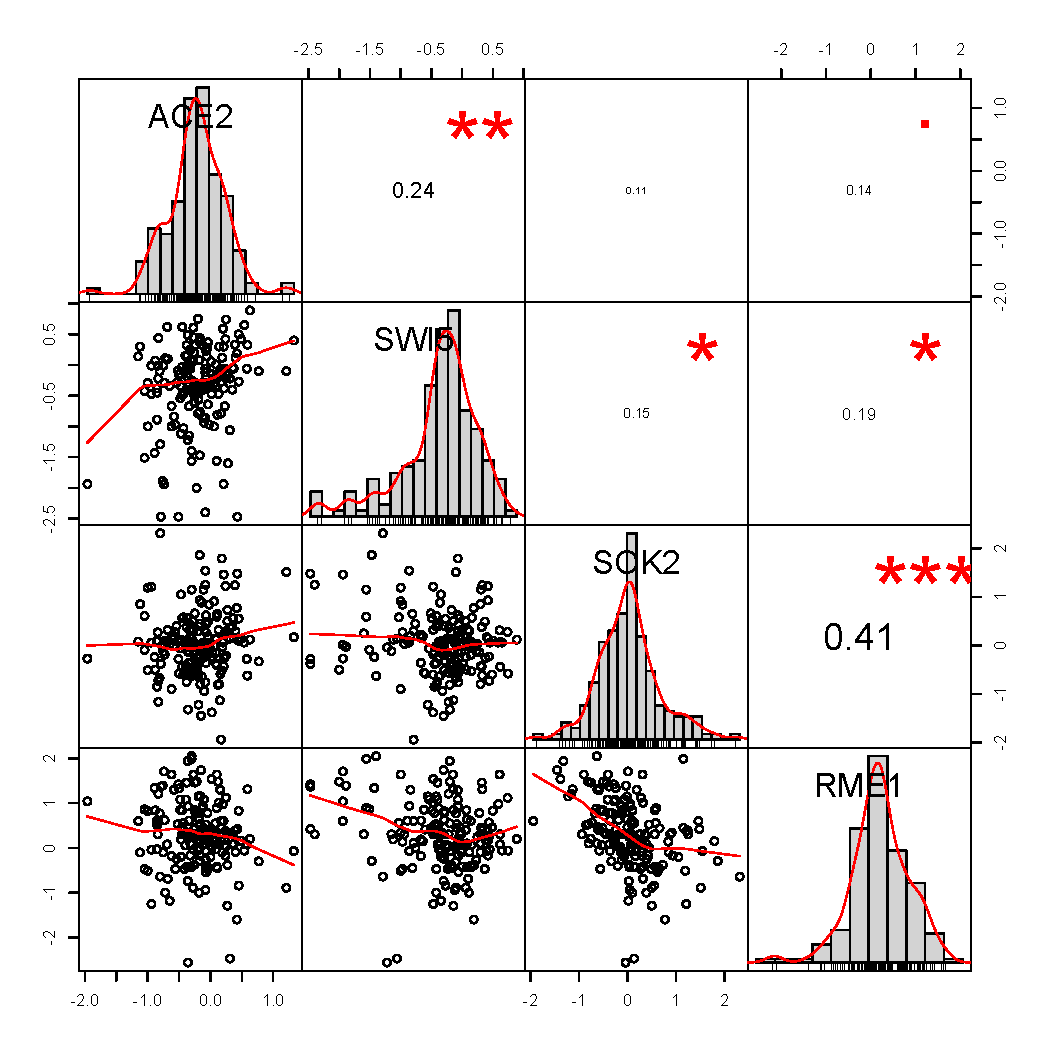
\includegraphics[width=0.5\columnwidth]{./figures/hands-on3/nice-pairs.pdf}
\caption{Output of the \lstinline!chart.Correlation()! function in the PerformanceAnalytics package, applied to the yeast expression data set.\label{fig:nicepairs}}
\end{figure}


% Here's an example based on code (see \href{http://gettinggeneticsdone.blogspot.com/2011/07/scatterplot-matrices-in-r.html}{this link} for the original source). Create a new R script called |mygraphs.R| and add the following function:
% %
% \begin{R}
% # panel.cor puts correlation in upper panels, size proportional to correlation
% panel.cor <- function(x, y, digits=2, prefix="", cex.cor, ...)
% {
%     usr <- par("usr"); on.exit(par(usr))
%     par(usr = c(0, 1, 0, 1))
%     r <- abs(cor(x, y))
%     txt <- format(c(r, 0.123456789), digits=digits)[1]
%     txt <- paste(prefix, txt, sep="")
%     if(missing(cex.cor))
%         cex.cor <- 0.8/strwidth(txt)
%     text(0.5, 0.5, txt, cex = cex.cor * r)
% }
% \end{R}
% You



\subsection{3D Scatter Plots}

A three-dimensional scatter plot can come in handy. The R library
\lstinline!lattice! has a function called \lstinline!cloud()! that
allows you to make such plots.
\begin{R}
> library(lattice)
> cloud(ACE2 ~ ASH1 * RAS2, data=yeast.clean)
> cloud(ACE2 ~ ASH1 * RAS2, data=yeast.clean, screen=list(x=-90, y=70)) # same plot from different angle
\end{R}
See the help file for \lstinline!cloud()! and \lstinline!panel.cloud()! for information on setting parameters.

\subsection{Scatterplot3D}
There is also a package available on CRAN called \lstinline!scatterplot3d! with similar functionality.
%
\begin{R}
> attach(yeast.clean) # so we can access the variables directly
> install.packages('scatterplot3d',dependencies=T) # installs scatterplot3d
> library(scatterplot3d) # assumes package is properly installed
> scatterplot3d(ASH1, RAS2, ACE2)
> scatterplot3d(ASH1, RAS2, ACE2, highlight.3d=T, pch=20,angle=25)
\end{R}
%
The |highlight.3d| argument colors points to help the viewer determine near and far points. Points that are closer to the viewer are lighter colors (more red in the default color scheme).

\subsubsection{Using Package Vignettes}
The Scatterplot3D package is quite flexible but this flexibility is hard to grok from the standard R help files (try |?scatterplot3d| to see for yourself).  Luckily the Scatterplot3D package includes a `vignette' -- a PDF document that discusses the design of the package and illustrates it's use.  Many packages include such vignettes. To see the list of vignettes available for your installed packages do the following:
%
\begin{R}
> vignette(all=T)
\end{R}
%
You should see that the vignette for the Scatterplot3D package is called |s3d|. You can access this vignette as follows, which should open the document in your default PDF viewer.
\begin{R}
> vignette("s3d")
\end{R}
%
In this case, the `good stuff' (i.e. the examples) starts on page 9 of the vignette.

\subsection{The rgl Package}

The 3D plots in |lattice| and |scatterplot3d| are fairly nice, but they don't allow the user to interact with the figures.  For example, wouldn't it be nice to be able to rotate a 3D scatter of points around to understand the relationships?  The |rgl| package allows you to do this, and can produce figures like that shown in Fig.~\ref{fig:rgl3d}.  Most R figures can be saved  using the |Save| option under the file menu. That's not the case for |rgl| plots. Instead we need to use the |rgl.postscript()| (creates a postscript or PDF version of the figure) or |snapshot3d()| (creates a screenshot) functions.
\begin{R}
> install.packages('rgl',dependencies=T)
> library(rgl)
> plot3d(ASH1, RAS2, ACE2, col='red', size=1, type='s')
> rgl.postscript('rgl3d-example.pdf', fmt='pdf')
\end{R}
%
\begin{figure}[htbp]
\centering
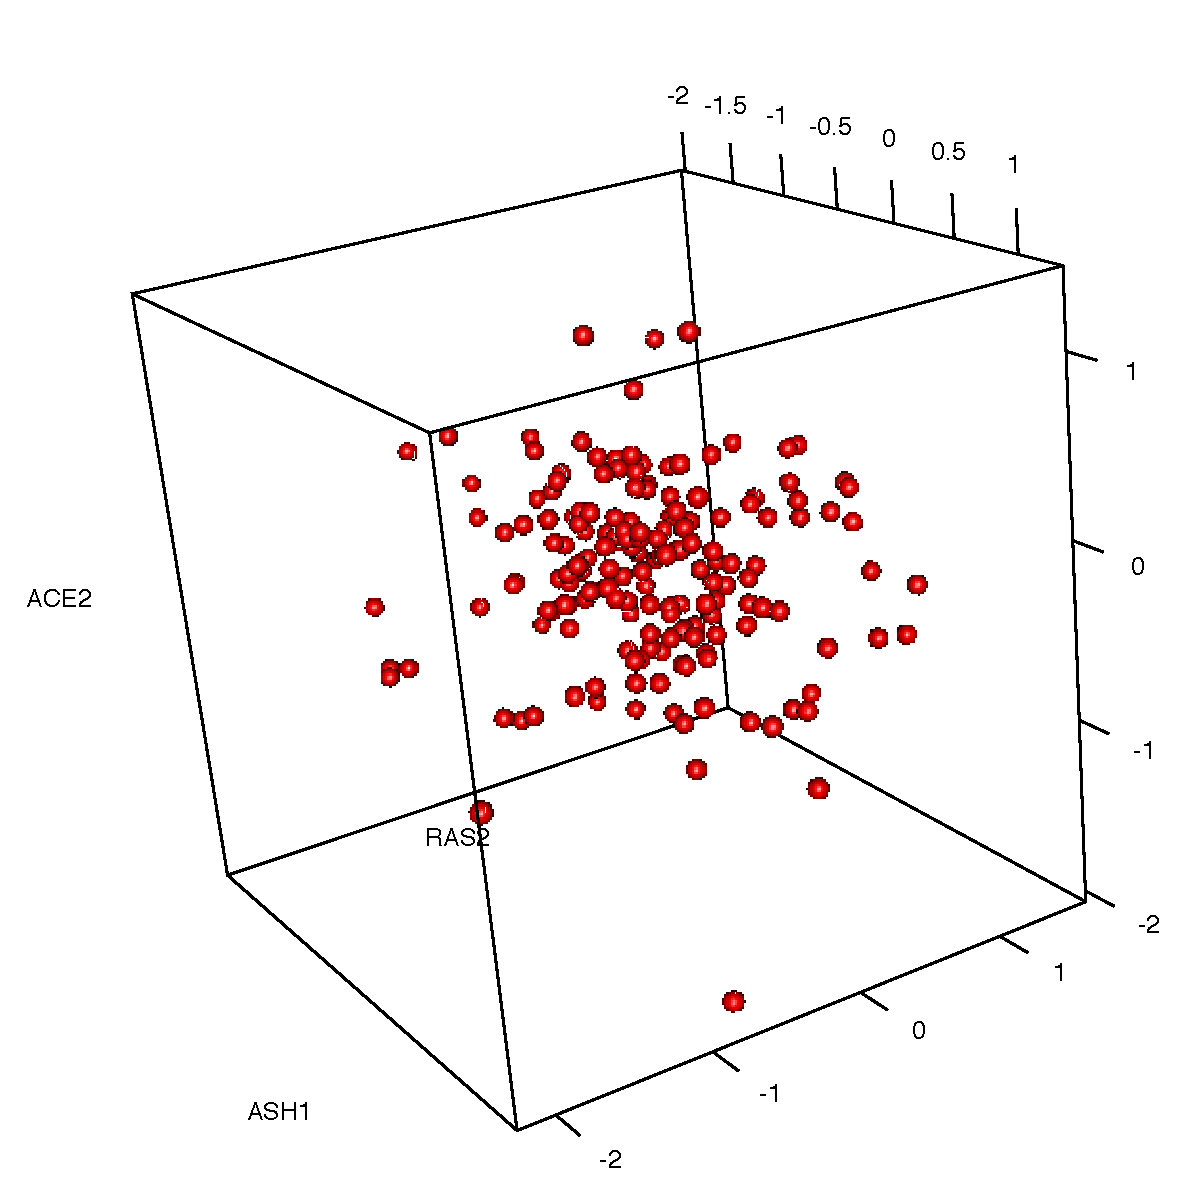
\includegraphics[width=0.5\columnwidth]{./figures/hands-on3/rgl3d-example.pdf}
\caption{Output of the \lstinline!plot3d()! function in the rgl package.\label{fig:rgl3d}}
\end{figure}

% Let's modify the 3D barplot on page 11 to create a 2D histogram. First we'll install another package -- |mvtnorm| -- that includes functions for creating multivariate normal distributions.
% %
% \begin{R}
% > install.packages('mvtnorm',dependencies=T)
% > library(mvtnorm)
% > ?rmvnorm # as always, check out the docs!

% \end{R}

\subsection{Colored grid plots}

A colored grid (or `heatmap') is another way of representing 3D data. It
most often is used to represent a variable of interest as a function of
two parameters. Grid plots can created using the \lstinline!image()!
function in R.

\begin{R}
> x <- seq(0, 2*pi, pi/20)
> y <- seq(0, 2*pi, pi/20)
> coolfxn <- function(x,y){
+    cos(x) * cos(y)}
> z <- outer(x,y,coolfxn) # the outer product of two matrices or vectors, see docs
> dim(z)
[1] 41 41
> image(x,y,z)
\end{R}
The \lstinline!x! and \lstinline!y! arguments to \lstinline!image()! are
vectors, the \lstinline!z! argument is a matrix (in this case created
using the outer product operator in conjunction with our function of
interest).

A somewhat more flexible function called |levelplot()| is found in the |lattice| package. For example, we can create a similar heatmap using |levelplot()| as follows:
\begin{R}
> library(lattice)
> levelplot(z)  # just the colors
> levelplot(z, contour=T) # colors plus contour lines
\end{R}
We can also apply the levelplot function to creat a representation of a correlation matrix, as shown here:
\begin{R}
> levelplot(cor(yeast.clean))
\end{R}
The default |levelplot()| colors are decent, but let's see how we can change the colors used to our liking. The |colorRampPalette()| function returns a function that interpolates between the values given as arguments to |colorRampPalette()|. So in the example below, it will create a series of colors from blue to white to red.
\begin{R}
> lvls <- seq(-1,1,0.1)  # set thresholds for our colors
> colors <- colorRampPalette(c('blue', 'white', 'red'))(length(lvls))
> levelplot(cor(yeast.clean), col.regions=colors, at=lvls)
\end{R}
%
The |colorRampPallete()| function can also take hexadecimal colors, as is commonly used in HTML. For a list of R colors see \url{http://research.stowers-institute.org/efg/R/Color/Chart/}.  For a  list of color schemes, developed by a geographer for effective cartographic representations,  see the \href{http://colorbrewer2.org/}{ColorBrewer web page}. For example, here's how to create the representation of the yeast data set correlation matrix shown in Fig.~\ref{fig:corrheat}:
\begin{R}
# this generates a color ramp from green to black to purple
> colors <- colorRampPalette(c('#1B7837', 'black', '#762A83'))(length(lvls))
> levelplot(cor(yeast.clean), col.regions=colors, at=lvls, scales=list(cex=0.6), xlab="", ylab="",main="Correlation Matrix\nYeast Expression Data")
\end{R}
The |scales| argument to |levelplot| changes the scaling of the tick marks and labels on the axes.

\begin{figure}[htbp]
\centering
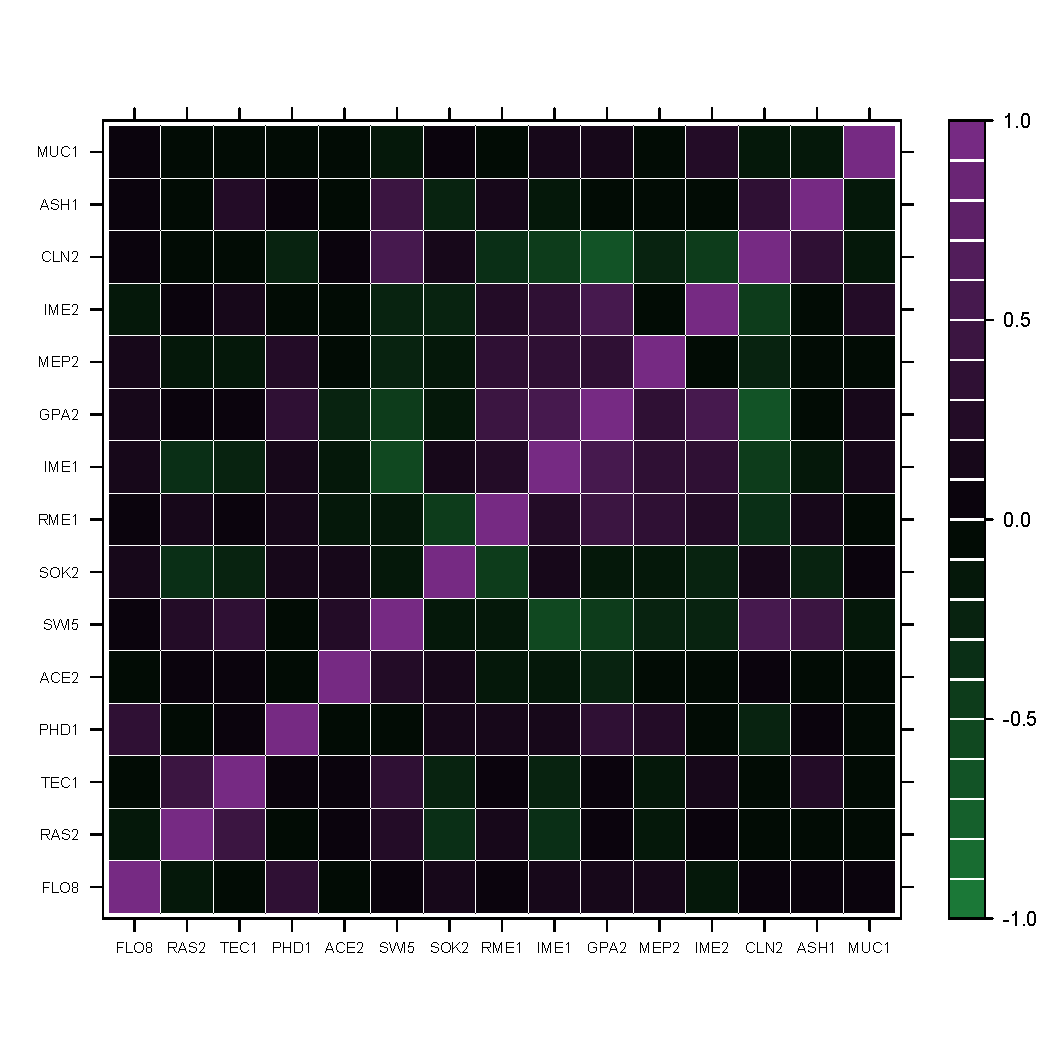
\includegraphics[width=0.5\columnwidth]{./figures/hands-on3/corr-heatmap.pdf}
\caption{A heatmap, representing the correlation matrix for the yeast expression data set, generated by the \lstinline!levelplot()! function in the lattice package.\label{fig:corrheat}}
\end{figure}


%
\section{Plotting in Python}

Python doesn't have any `native' data plotting tools but there are a
variety of packages that provide tools for visualizing data. The package
we're going to use is called `Matplotlib'. Matplotlib is one of the many
packages that is distributed with the Enthought Python distribution. If
you want to explore the full power of Matplotlib check out the example
gallery and the documentation at
\url{http://matplotlib.sourceforge.net/}.

\subsection{Basic plots using matplotib}

If you invoked the Ipython shell using the pylab option than most of the
basic matplotlib functions are already available to you. If not, import
them as so:

\begin{python}
>>> from pylab import *
>>> import numpy as np # go ahead and import numpy as well
\end{python}
\subsubsection{Loading data}

First let's load the yeast data set:

\begin{python}
>>> data = np.loadtxt('yeast-subnetwork-clean.txt',skiprows=1,usecols=range(1,16))
>>> data.shape   # check the dimensions of the resulting matrix
(173, 15)
\end{python}
The \lstinline!skiprows! argument tells the function how many rows in
the data file you want to skip. In this case we skipped only the first
row which gives the variable names. The \lstinline!usecols! arguments
specificies which columns from the data file to use. Here we skipped the
first (zeroth) column which had the names of the conditions. The usecols
\lstinline!loadtxt! works when there is no missing data. Use
\lstinline!numpy.genfromtxt! instead when there are missing values. For
a full tutorial on how to use the \lstinline!numpy.genfromtxt! function
see
\url{http://docs.scipy.org/doc/numpy/user/basics.io.genfromtxt.html}.

\subsubsection{Histograms in Matplotlib}

Matplotlib has a histogram drawing function. Here's how to use it:

\begin{python}
>>> hist? # in Ipython calls the help function
>>> h = hist(data[:,0]) # plot a histogram of the first variable (column) in our data set
>>> clf() # clear the plot window, don't need this if you closed the plot window
>>> h = hist(data[:,0], bins=20) # plot histogram w/20 bins
>>> h = hist(data[:,:2])  # histograms of the first two variables    
\end{python}
There's no built in density plot function, but we can create a function
that will do the necessary calculations for us to create our own density
plot. This uses a kernel density estimator function in the scipy library
(included with EPD). Put the following code in a file called
\lstinline!myplots.py! somewhere on your \lstinline!PYTHONPATH!:

\begin{python}
# myplots.py

import numpy as np
from scipy import stats

def density_trace(x):
    kde = stats.gaussian_kde(x)
    xmin,xmax = min(x), max(x)
    xspan = xmax - xmin
    xpts = np.arange(xmin, xmax, xspan/1000.)
    ypts = kde.evaluate(xpts) # evalude the estimate at the xpts
    return xpts,ypts
\end{python}
You can then use the \lstinline!density_trace! function as follows:

\begin{python}
>>> import myplots
>>> h = hist(data[:,0], normed=True) # use normed=True so histogram 
                           # is normalized to form a prob. density
>>> x,y = myplots.density_trace(data[:,0])
>>> plot(x,y, 'red')    
\end{python}
\subsubsection{Boxplots in Matplotlib}

Box-and-whisker plots are straightforward in Matplotlib:

\begin{python}
>>> b = boxplot(data[:,0])
>>> clf()
>>> b = boxplot(data[:,:5]) # boxplots of first 5 variables
\end{python}
The \lstinline!boxplot! function has quite a few facilities for
customizing your boxplots. For example, here's how we can create a
notched box-plot using 1000 bootstrap replicates (we'll discuss the
bootstrap in more detail in a later lecture) to calculate confidence
intervals for the median.

\begin{python}
>>> boxplot(data[:,0], notch=1, bootstrap=True)    
\end{python}
See the Matplotib docs for more info.

\subsubsection{Scatter Plots in Matplotlib}

Scatter plots are also easy to create:

\begin{python}
>>> s = scatter(data[:,0], data[:,1])    
\end{python}
\subsection{3D Plots}

Recent version of Matplotlib include facilities for creating 3D plots.
Here's an example of a 3D scatter plot:

\begin{python}
>>> from mpl_toolkits.mplot3d import Axes3D
>>> fig = figure()
>>> ax = fig.add_subplot(111, projection = '3d')
>>> ax.scatter(data[:,0],data[:,1],data[:,2])
<mpl_toolkits.mplot3d.art3d.Patch3DCollection object at 0x1a0bbd70>
>>> ax.set_xlabel('Gene 1')
<matplotlib.text.Text object at 0x1a0ae7d0>
>>> ax.set_ylabel('Gene 2')
<matplotlib.text.Text object at 0x1a0bb2b0>
>>> ax.set_zlabel('Gene 3')
<matplotlib.text.Text object at 0x1a0bbcd0>
>>> show()
\end{python}
Retyping all those commands is tedious and error prone so let's turn it
into a function. Add the following code to \lstinline!myplots.py!:

\begin{python}
from matplotlib import pyplot
from mpl_toolkits.mplot3d import Axes3D

def scatter3d(x,y,z, labels=None):
    fig = pyplot.figure()
    ax = fig.add_subplot(111, projection='3d')
    ax.scatter(x,y,z)

    if labels is not None:
        try:
            ax.set_xlabel(labels[0])
            ax.set_ylabel(labels[1])
            ax.set_zlabel(labels[2])
        except IndexError:
            print "You specificied less than 3 labels."
    return fig
\end{python}
Now reload myplots and call the scatter3d function as so:

\begin{python}
>>> reload(myplots)
>>> myplots.scatter3d(data[:,0], data[:,1], data[:,2])
>>> myplots.scatter3d(data[:,0], data[:,1], data[:,2], lab)
>>> myplots.scatter3d(data[:,0], data[:,1], data[:,2],labels=('X','Y','Z'))
\end{python}
\section{Plotting Geographic Data using Basemap}

There are a number of toolkits available for Matplotlib that extend the
functionality of the package. The mplot3d is one of those toolkits which
has now been incorporated into the standard distribution. Basemap is
another toolkit that provides the ability to plot 2D data on maps. The
Basemap toolkit supports a variety of mapping projections and coordinate
transformations and has the ability to plot things likes water bodies
and political boundaries.

The EPD edition of Python includes Basemap but in the interest of space
they have removed the high resolution maps that the normal Basemap
distribution includes. In order to use those maps you can download a
basemap binary (for Windows) or the source code (on OS X) from the
\href{http://sourceforge.net/projects/matplotlib/files/matplotlib-toolkits/basemap-1.0.1/}{here}.

On Windows just run the executable installer (make sure you get the
version that is appropriate to your EPD distribution; either 32-bit or
64-bit).

On OS X, once you have downloaded the source tarball
(\lstinline!basemap-1.0.1.tar.gz!), open up a bash shell, navigate to
the directory where you saved the tarball, and type:

\begin{python}[language=bash]
tar xvzf basemap-1.0.1.tar.gz
\end{python}
This will decompress and unarchive the source code into a directory
called \lstinline!basemap-1.0.1!. Navigate to the directory where the
mapping data is stored:

\begin{python}[language=bash]
cd basemap-1.0.1/lib/mpl_toolkits/basemap/data
\end{python}
And then copy all the \lstinline!.dat! files to your Python
installation:

\begin{python}[language=bash]
cp *.dat /Library/Frameworks/Python.framework/Versions/Current/lib/python2.7/site-packages/mpl_toolkits/basemap/data
\end{python}
\subsection{Using Basemap}

In our first basemap example we show how to plot the US lower 48 and we
add a red dot to represent the city of Durham, NC. Save this code as
\lstinline!mapex.py! and run it from the command line
(\lstinline!python mapex.py!).

\begin{codeblock}[python]
# Derived from: Tosi, Sandro. Plotting Geographical Data using Basemap
# url: http://www.packtpub.com/article/plotting-geographical-data-using-basemap

import numpy as np
from matplotlib import pyplot
from mpl_toolkits.basemap import Basemap

# Lambert Conformal map of USA lower 48 states
m = Basemap(llcrnrlon=-119, llcrnrlat=22, urcrnrlon=-64,
  urcrnrlat=49, projection='lcc', lat_1=33, lat_2=45,
  lon_0=-95, resolution='l', area_thresh=10000)

# draw the coastlines of continental area
m.drawcoastlines()
# draw country boundaries
m.drawcountries(linewidth=2)
# draw states boundaries (America only)
m.drawstates()

# fill the background (the oceans)
m.drawmapboundary(fill_color='aqua')
# fill the continental area and lakes
m.fillcontinents(color='coral',lake_color='aqua')

# draw pt. indicating durham/raleigh area
# Durham, latitude:  35deg 52min N, longitude:78deg 47min W
dlat, dlong = 35.86, -78.78 # west is minus

# this maps latitude and longitude to map coordinates
mcoordx, mcoordy = m(dlong,dlat)
pyplot.plot(mcoordx,mcoordy, 'ro') # draw red dot
pyplot.text(mcoordx+36000, mcoordy-18000, 'Durham')

# finally show the file
pyplot.show()    
\end{codeblock}
%
In our second example let's assume you've been studying the population
genetics of the beautiful and rare North Carolina Blue Snouter (mammals
of the order Rhinogradentia; see Stümpke 1967. The snouters: form and
life of the Rhinogrades). You've been sampling snouter populations from
across NC and you want to make a figure for a paper showing all your
sampling locations. Download the file \lstinline!nc-sites.txt! from the
course wiki, and place it in the same directory as the following module
(\lstinline!mapex2.py!).

\begin{codeblock}[python]
# mapex2.py

import numpy as np
from matplotlib import pyplot
from mpl_toolkits.basemap import Basemap

m = Basemap(llcrnrlon=-85, llcrnrlat=33, urcrnrlon=-75,
  urcrnrlat=37, projection='lcc', lat_0=35.774, lon_0=-78.634,
  resolution='l', area_thresh=10000)

m.drawcoastlines()
m.drawcountries(linewidth=2)
m.drawstates()
m.drawmapboundary(fill_color='aqua')
m.fillcontinents(color='coral',lake_color='aqua')

sites = np.loadtxt('nc-sites.txt')

for row in sites:
    lat, lon = row[0], row[1]
    x,y = m(lon, lat) # note how longitude (x-direction) comes first
    # use blue +'s to plot sites
    pyplot.plot(x,y, 'b+', markersize=8,markeredgewidth=2) 

pyplot.show()    
\end{codeblock}
%
The \lstinline!mapex2.py! code will produce a figure like the one below.

\begin{figure}[htbp]
\centering
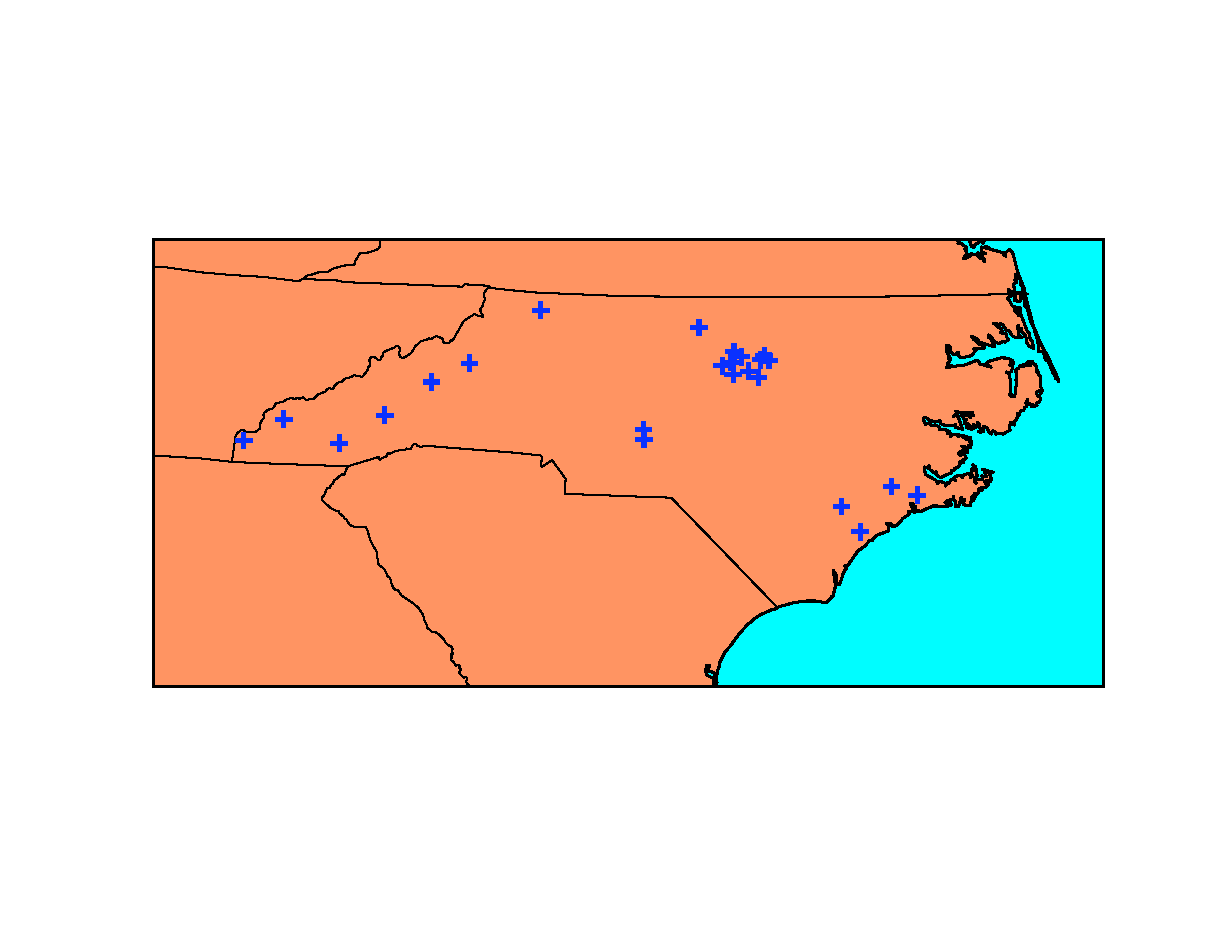
\includegraphics[width=0.6\columnwidth]{./figures/hands-on3/mapfig.pdf}
\caption{Output of the mapex2.py module}
\end{figure}






\chapter{Multiple Regression in R}
% \section{Introduction to Literate Programming Using knitr}



|knitr| documents weave together documentation/discussion and code into a
single document. The pieces of code and documentation are referred to as
`chunks'. Using |knitr| you can turn the entire document into a nicely formatted report, or you can extract just the code parts.

I recommend you use |knitr| from inside RStudio, which has a Markdown aware editor and is pre-configured to compile |knitr| documents into HTML. The first thing you'll need to do is install the |knitr| and |markdown| packages, either from the command line using|install.packages()| or from the |Tools > Install Packages| menu (make sure you include the dependencies). Once you've installed |knitr| you can create a Markdown document using |File > New > R Markdown|.

RStudio gives you a template  file that illustrates the basic Markdown syntax.  For more info about Markdown click the `MD' button, which will bring up a quick reference guide.  Replace the template with the following, and save it as |knitr1.Rmd|. Note that the |.Rmd| extension is recognized by RStudio as an R markdown file. I suggest that you get in the habit of using this extension for your markdown files.

\begin{codeblock}
# Getting started with knitr

This is a very simple knitr Markdown file. It includes only a single
code chunk.

```{r}
z <- rnorm(30, mean=0, sd=1)
summary(z)
```

The code chunk above generated a random sample of 30 observations
drawn from a normal distribution with mean zero and standard
deviation one.
\end{codeblock}

Let's break down the various pieces of the document. The first line is a header.  |#| generates a level one header, |##| generates a level two header, etc.  This header is than followed by a couple of lines of text, which will appear in the output.

The R code chunk begins and ends with sets of three backticks.  The |{r}| immediately after the first set of backticks tells knitr to treat  the code as R code (you can also process other languages such as Python). The final set of backticks tells knitr that you're going back to writing documentation
chunks.

After saving your document you can compile it using the |Knit HTML| button or from the R console as:
\begin{R}
> library(knitr)
> knit2html('knit1.Rmd')
\end{R}
%
Either of the above approaches will generate two new file |knit1.md| and |knit1.html|. RStudio will automatically open the HTML file in a built-in viewer, or you can open the HTML file in any browser. Notice how the code from the code chunk is in the output file as well as the output that you would have generated had you typed the code in at the R console.


\subsection{A fancier knitr document}

Let's get a little bit fancier and show how we can create graphics and
use some Markdown formatting features to produce a nicer document.
%
\begin{codeblock}
# My Second knitr Report
# John Q. Public

This is a still a simple knitr document. However,
now it includes several code chunks and several
markdown formatting commands.

## Sampling from the random normal distribution

```{r}
z <- rnorm(30, mean=0, sd=1)
summary(z)
```

That code chunk generated a random sample of 30
observations drawn from a normal distribution with mean
zero ($\mu = 0$) and standard deviation one ($\sigma = 1$).


### Generating figures#

We can also automatically imbed graphics in our
report. For example, the following will generate
a histogram.

```{r fig=TRUE, fig.width=4, fig.height=4}
hist(z)
```
\end{codeblock}

In the second document chunk we included some text between dollar signs.  knitr recognizes this as mathematical text, using \LaTeX\ based formatting. Also notice how we put an argument, \lstinline!fig=TRUE! within the second
code chunk delimiter. This will tell knitr to automatically imbed a
figure with the histogram graphic we created into our report.  We also specified the dimensions of this figure using |fig.width| and |fig.height|.  Save the document
as \lstinline!knit2.Rmd! and repeat the above steps to compile it into
a PDF report.

For a full overview of knitr's capabilities see the documentation for
knitr availabe at
\url{http://yihui.name/knitr/}.




\section{Multiple Regression in R}

To illustrate multiple regression in R we'll use a built in dataset called |trees|. |trees| consists of measurements of the girth, height, and volume of 31 black cherry trees (|?trees| for more info). We'll start with some summary tables and diagnostic plots to familiarize ourselves with the data:
%
\begin{R}
> names(trees)
[1] "Girth"  "Height" "Volume"
> dim(trees)
[1] 31  3
> summary(trees)
     Girth           Height       Volume
 Min.   : 8.30   Min.   :63   Min.   :10.20
 1st Qu.:11.05   1st Qu.:72   1st Qu.:19.40
 Median :12.90   Median :76   Median :24.20
 Mean   :13.25   Mean   :76   Mean   :30.17
 3rd Qu.:15.25   3rd Qu.:80   3rd Qu.:37.30
 Max.   :20.60   Max.   :87   Max.   :77.00

# we'll use the chart.Correlation fxn that we introduced last week 
> library(PerformanceAnalytics)  
> chart.Correlation(trees)
\end{R}
%
As one might expect, the scatterplot matrix shows that all the variables are positively correlated, and girth and volume have a  particularly strong correlation.

Let's assume we're lumberjacks, but our permit only allows us to harvest a fixed number of trees.  We get paid by the total volume of wood we harvest, so we're interested in predicting a tree's volume (hard to measure directly) as a function of its girth and height (relatively easy to measure), so we can pick the best trees to harvest.  We'll therefore calculate a multiple regression of volume on height and width. Let's start by taking a look at the 3D scatter of the data using the plot3d function from the |rgl| package.
%
\begin{R}
> library(rgl)
> plot3d(trees, col='red', size=1, type='s') # use your mouse to rotate the plot
\end{R}
%
From the 3D scatter plot it looks like we ought to be able to find a plane through the data that fits the scatter fairly well. Let's use the |lm()| function to calculate the multiple regression:
%
\begin{R}
> l <- lm(Volume ~ Girth + Height, data=trees)
\end{R}
%
To visualize the multiple regression, let's use the |scatterplot3d| package to draw the 3D scatter of plots and the plane that corresponds to the regression model:
%
\begin{R}
> library(scatterplot3d)  # install this package first if needed
> p <- scatterplot3d(trees,angle=55,type='h')
> title('Tree Volume as\na function of Girth and Height')
> p$plane3d(l, col='orangered')
> dev.copy(pdf, 'trees-regrfit.pdf')  # copy plot to a pdf file
> dev.off()  # write the file
\end{R}
%
Notice the use of |dev.copy()| and |dev.off()| to save the plot from the console.  The output this generates should look similar to Fig.~\ref{fig:treesregr}.
%
\begin{figure}[htbp]
\centering
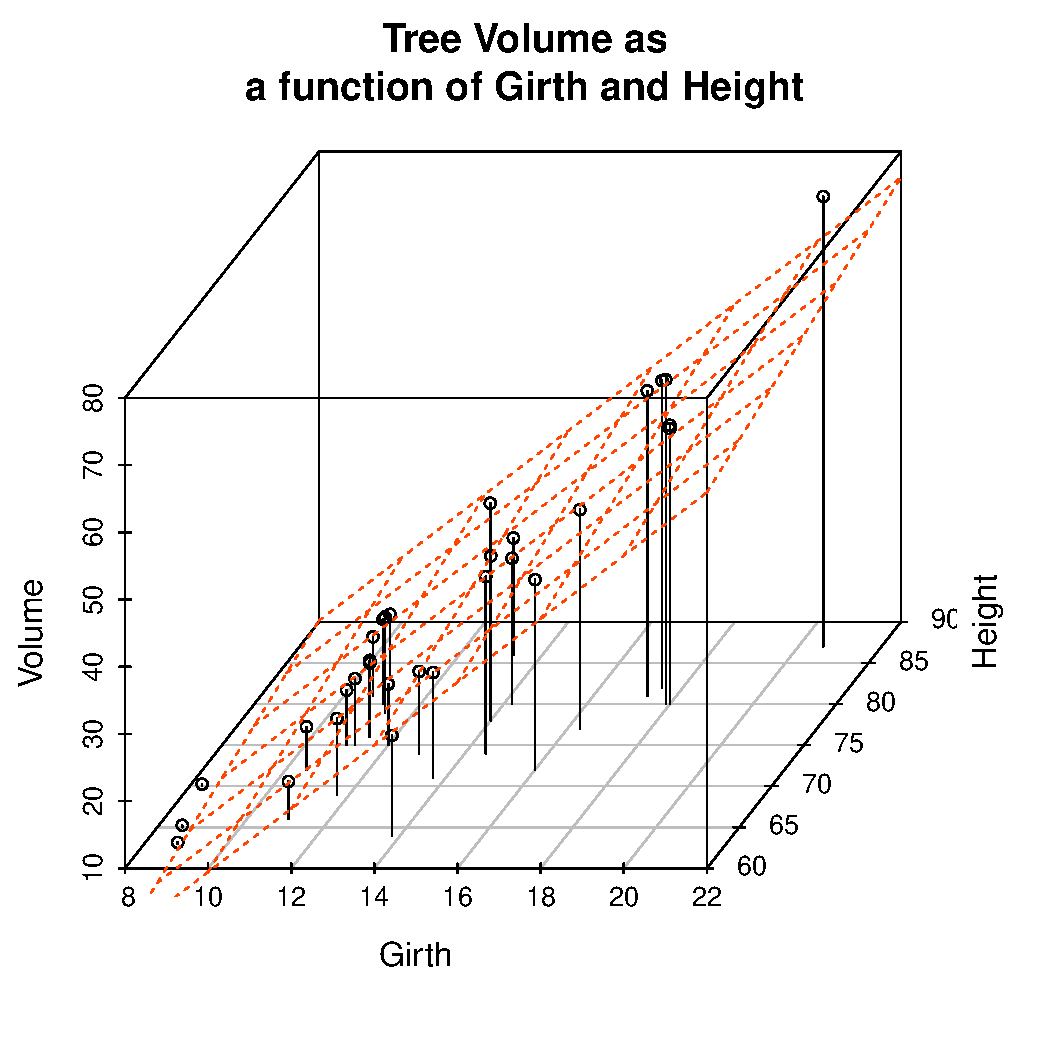
\includegraphics[width=0.5\columnwidth]{./figures/hands-on4/trees-regrfit.pdf}
\caption{Multiple regression plot of cherry tree volume on girth and height, generated using the \texttt{scatterplot3d} library\label{fig:treesregr}}
\end{figure}

From the figure it looks like the regression model fits pretty well, as we anticipated  from the pairwise relationships.  Let's use the |summary()| function to obtain details of the model:
\begin{R}
> summary(l)

Call:
lm(formula = Volume ~ Girth + Height, data = trees)

Residuals:
    Min      1Q  Median      3Q     Max
-6.4065 -2.6493 -0.2876  2.2003  8.4847

Coefficients:
            Estimate Std. Error t value Pr(>|t|)
(Intercept) -57.9877     8.6382  -6.713 2.75e-07 ***
Girth         4.7082     0.2643  17.816  < 2e-16 ***
Height        0.3393     0.1302   2.607   0.0145 *
---
Signif. codes:  0 ‘***’ 0.001 ‘**’ 0.01 ‘*’ 0.05 ‘.’ 0.1 ‘ ’ 1

Residual standard error: 3.882 on 28 degrees of freedom
Multiple R-squared: 0.948,  Adjusted R-squared: 0.9442
F-statistic:   255 on 2 and 28 DF,  p-value: < 2.2e-16
\end{R}
%
The regression equation is: $\hat{y} = 4.71x_1 + 0.34x_2$, where $y$ is Volume, and $x_1$ and $x_2$ are Girth and Height respectively. Since they're on different scales the coefficients for Girth and Height aren't directly comparable. Both coefficients are significant at the $p<0.05$ level, but note that Girth is the much stronger predictor. In fact the addition of height explains only a minor additional fraction of variation in tree volume, so from the lumberjack's perspective the additional trouble of measuring height probably isn't worth it.

\subsection{Exploring the Vector Geometry of a Regression Model}

The object returned by the |lm()| function hold lots of useful information:
%
\begin{R}
> names(l)
 [1] "coefficients"  "residuals"     "effects"       
     "rank"          "fitted.values" "assign"
 [7] "qr"            "df.residual"   "xlevels" 
     "call"          "terms"         "model"
\end{R}
%
The |fitted.values| correspond to the predicted values of the outcome variable ($\hat{y}$). Let's use our knowledge of vector geometry to further explore the relationship between the predicted Volume and the predictor variables.  By definition the vector representing the predicted values lies in the plane defined by Height and Girth, so let's do some simple calculations to understand their length and angular relationships:
%
\begin{R}
# proportional to length of vectors
> sd(l$fitted.values)
[1] 16.00434
> sd(trees$Height)
[1] 6.371813
> sd(trees$Girth)
[1] 3.138139

# cosines of angles btw vectors
> cor(trees$Height, trees$Girth)
[1] 0.5192801
> cor(trees$Height, l$fitted.values)
[1] 0.6144545
> cor(trees$Girth, l$fitted.values)
[1] 0.9933158

# angles btw vectors in degrees
> acos(cor(trees$Height, l$fitted.values)) * (180/pi)
[1] 52.08771
> acos(cor(trees$Girth, l$fitted.values)) * (180/pi)
[1] 6.628322
> acos(cor(trees$Girth, trees$Height)) * (180/pi)
[1] 58.71603
\end{R}
%

\begin{tcolorbox}[title=In class assignment]
Using the calculations above you should now be able to sketch out by hand, a diagram depicting the vector relationships between Height, Girth, and the predicted Volume .  Once you've finished with your sketch, discuss it with your fellow classmates.  Did you get similar answers? If not, discuss it and try to come up with an agreed upon representation.
\end{tcolorbox}

\subsection{Exploring the Residuals from the Model Fit}

Now let's look at the residuals from the regression. The residuals represent the `unexplained' variance:
\begin{R}
> plot(trees$Volume,l$residuals, xlab='Volume',ylab='Regression Residuals')
> abline(h=0, lty='dashed', col='red')
\end{R}
%
Ideally the residuals should be evenly scattered around zero, with no trends as we go from high to low values of the dependent variable.  As you can see in Fig.~\ref{fig:trees-resid} it looks like that the residuals on the left tend to be below zero, while those on the far right of the plot are consistently above zero, suggesting that there may be a non-linear aspect of the relationship that our model isn't capturing.
%
\begin{figure}[htbp]
\centering
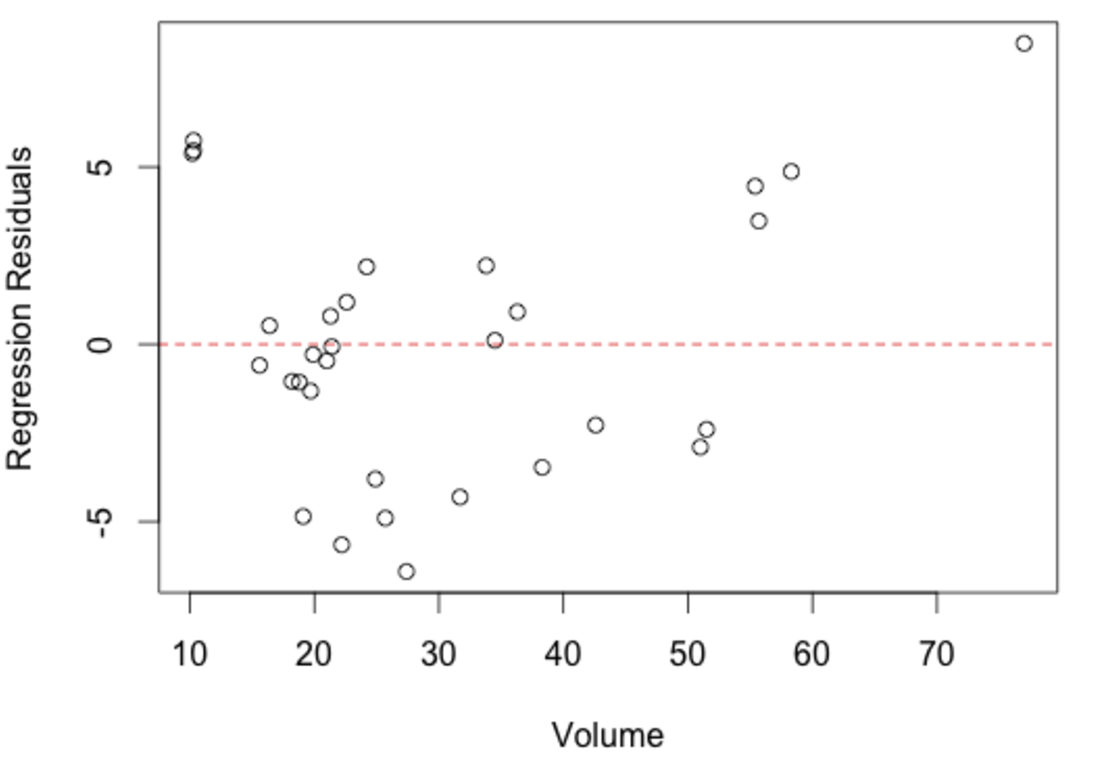
\includegraphics[height=1.5in]{./figures/hands-on4/trees-residuals.pdf}
\caption{Residual plot based on the multiple regression plot of cherry tree volume on girth and height,\label{fig:trees-resid}}
\end{figure}

Let's think about the relationships we're actually modeling for a few minutes.  For the sake of simplicity let's consider the trunk of a tree to be a cylinder.  How do the dimensions of this cylinder relate to its volume? You can look up the formula for the volume of a cylinder, but the key thing you'll want to note is that volume of the cylinder should be proportional to a characteristic length of the cylinder cubed ($V \propto \mathrm{L}^3$). This suggests that if we want to fit a linear model we should relate Girth to $\sqrt[3]{\mathrm{Volume}}$. Let's explore this a little. Since our initial multiple regression suggested that height had relatively little predictive power, we'll simplify our model down to a single predictor:
%
\begin{R}
> cuberoot.V <- trees$Volume^0.33
> cor(trees$Volume, trees$Girth)
[1] 0.9671194
> cor(cuberoot.V, trees$Girth)
[1] 0.9777078
> l.orig <- lm(trees$Volume~ trees$Girth)
> l.transf <- lm(cuberoot.V ~ trees$Girth)
> summary(l.orig)

Call:
lm(formula = trees$Volume ~ trees$Girth)

Residuals:
   Min     1Q Median     3Q    Max
-8.065 -3.107  0.152  3.495  9.587

Coefficients:
            Estimate Std. Error t value Pr(>|t|)
(Intercept) -36.9435     3.3651  -10.98 7.62e-12 ***
trees$Girth   5.0659     0.2474   20.48  < 2e-16 ***
---
Signif. codes:  0 ‘***’ 0.001 ‘**’ 0.01 ‘*’ 0.05 ‘.’ 0.1 ‘ ’ 1

Residual standard error: 4.252 on 29 degrees of freedom
Multiple R-squared: 0.9353, Adjusted R-squared: 0.9331
F-statistic: 419.4 on 1 and 29 DF,  p-value: < 2.2e-16

> summary(l.transf)

Call:
lm(formula = cuberoot.V ~ trees$Girth)

Residuals:
     Min       1Q   Median       3Q      Max
-0.18919 -0.09775 -0.01488  0.07855  0.26427

Coefficients:
            Estimate Std. Error t value Pr(>|t|)
(Intercept)  0.82543    0.08856   9.321 3.18e-10 ***
trees$Girth  0.16324    0.00651  25.076  < 2e-16 ***
---
Signif. codes:  0 ‘***’ 0.001 ‘**’ 0.01 ‘*’ 0.05 ‘.’ 0.1 ‘ ’ 1

Residual standard error: 0.1119 on 29 degrees of freedom
Multiple R-squared: 0.9559, Adjusted R-squared: 0.9544
F-statistic: 628.8 on 1 and 29 DF,  p-value: < 2.2e-16
\end{R}
%
Comparing the summary tables, we see indeed that using the cube root of Volume improves the fit of our model some. Let's examine the residuals.
%
\begin{R}
> layout(c(1,2), widths=c(3,3), heights=c(2,2))
> plot(trees$Volume, l.orig$residuals, xlab='Volume', ylab="Residuals")
> abline(h = 0, col='red', lty='dashed')
> plot(cuberoot.V, l.transf$residuals, 
        xlab='Volume^0.33', ylab='Residuals')

> abline(h = 0, col='red', lty='dashed')
> dev.copy(pdf, 'compare-residuals.pdf')
> dev.off()
> layout(c(1,1))   # reset the layout
\end{R}
%
\begin{figure}[htbp]
\centering
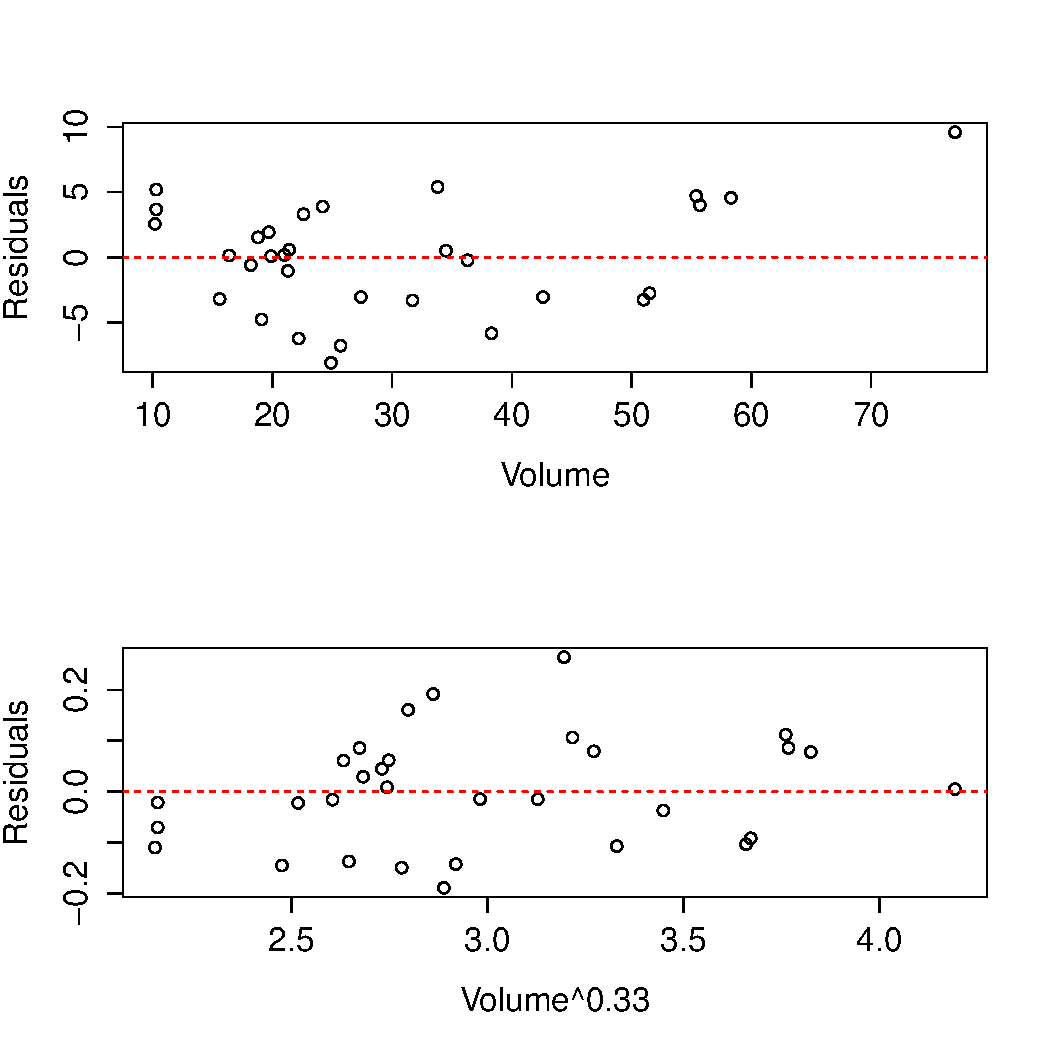
\includegraphics[height=2in]{./figures/hands-on4/compare-residuals.pdf}
\caption{Residual plot based on the bivariate regression of tree volume on girth, or $\sqrt[3]{V}$ on girth \label{fig:compare-resid}}
\end{figure}
%
As we can see the transformation we applied to the data did seem to make our residuals more uniform across the range of observations. Note the use of the |layout()| function to put multiple plots in the same figure.

\subsection{Fitting a curvilinear model using lm()}

Above we transformed the volume data in order to fit a straight line relationship between $\sqrt[3]{V}$  and Girth. However, we could just as easily have applied a cubic regression to the original variables as shown below (remember this is still linear  in the coefficients):

\begin{R}
> lm.3 <- lm(Volume ~ I(Girth^3), data=trees)
> summary(lm.3)

Call:
lm(formula = Volume ~ I(Girth^3), data = trees)

Residuals:
   Min     1Q Median     3Q    Max
-4.526 -3.036  0.215  2.419  8.291

Coefficients:
             Estimate Std. Error t value Pr(>|t|)
(Intercept) 8.0426960  1.0426698   7.714 1.66e-08 ***
I(Girth^3)  0.0081365  0.0003118  26.098  < 2e-16 ***
---
Signif. codes:  0 ‘***’ 0.001 ‘**’ 0.01 ‘*’ 0.05 ‘.’ 0.1 ‘ ’ 1

Residual standard error: 3.379 on 29 degrees of freedom
Multiple R-squared: 0.9592, Adjusted R-squared: 0.9578
F-statistic: 681.1 on 1 and 29 DF,  p-value: < 2.2e-16

> lm.3$coefficients
(Intercept)  I(Girth^3)
8.042696007 0.008136533
> a0 = lm.3$coefficients[[1]]
> B1 = lm.3$coefficients[[2]]
> x <- seq(8,25,0.25) # range of values to evaluate model over
> fit <- a0 + B1*x^3
> plot(Volume ~ Girth, data=trees)
> lines(x,fit,col='red')
> figtext <- paste(c("Volume = ", round(a0,2), "+", round(B1,4), "*Girth^3"), collapse='')
> text(12, 60, figtext)
\end{R}
%
\begin{figure}[htbp]
\centering
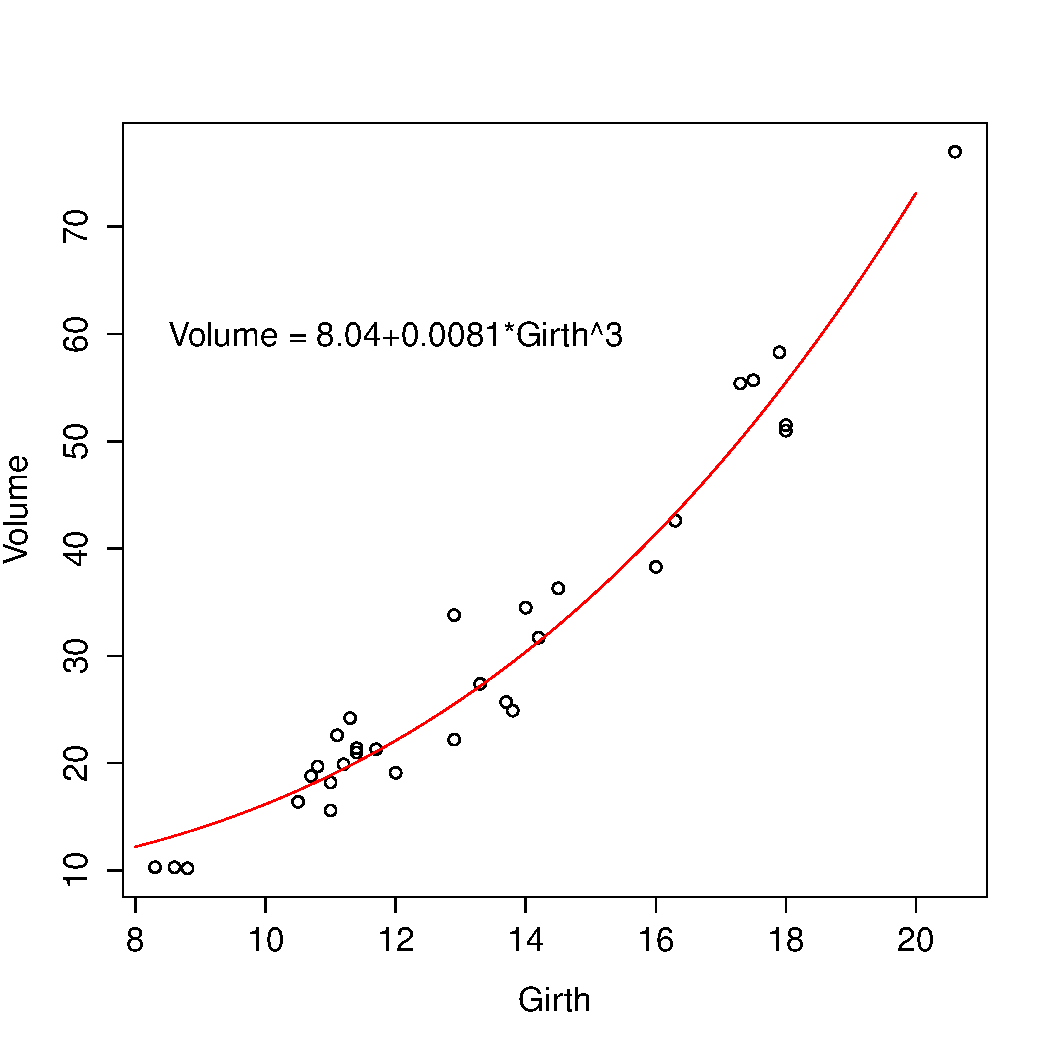
\includegraphics[height=2in]{./figures/hands-on4/cubic-regr.pdf}
\caption{Cubic regression of tree volume on girth \label{fig:cubic-regr}}
\end{figure}
%
The |I()| function used above requires a little explanation.  Normally, the R formula syntax (see |?formula|) treats the carat symbol, |'^'|, as short-hand for factor crossing to the specified degree.  For example, the formula |(a+b+c)^2| would be interpretted as the model with main effects and all second order interaction terms, i.e. |a + b + c + a:b + a:c + b:c| where the colons indicate interactions.  The |I()| function `protects' the object in it's argument; in this case telling the regression function to treat this as Girth raised to the third power as opposed to trying to construct interaction terms for Girth.


\medskip
\begin{assignment}
Write a function, |mult.regr(X,y)| that calculates the multiple regression of $y$ on multiple predictors, $x_1, x_2, \ldots x_k$ \emph{using matrix operations}. Your function should take two arguments, |X| and |y|, where |X| is a matrix representing the predictor variables and |y| is a vector for the outcome variable.  Your function should return a list containg the vector of regression coeffients, $B$, the coefficient of determination ($R^2$), and a vector, $\hat{y}$, representing the fitted values.  Refer to the slides from lecture 4 (and possibly lecture 2 if you need a refresher) to review the matrix  solution to the regression problem.
\end{assignment}


\section{Exploring the impact of nearly collinear predictors on regression}

In lecture we discussed the problems that can arise in regression when your predictor variables are nearly collinear. In this section we'll illustrate some of these issues.

Consider again the |trees| data set.  Recall that two of the variables -- Girth and Volume -- are highly correlated and thus nearly collinear.
%
\begin{R}
> cor(trees)
           Girth    Height    Volume
Girth  1.0000000 0.5192801 0.9671194
Height 0.5192801 1.0000000 0.5982497
Volume 0.9671194 0.5982497 1.0000000
\end{R}
%
Let's explore what happens when we treat Height as the dependent variable, and Girth and Volume as the predictor variables.
%
\begin{R}
> lm.H <- lm(Height ~ Girth + Volume, data = trees)
> summary(lm.H)

Call:
lm(formula = Height ~ Girth + Volume, data = trees)

Residuals:
    Min      1Q  Median      3Q     Max 
-9.7855 -3.3649  0.5683  2.3747 11.6910 

Coefficients:
            Estimate Std. Error t value Pr(>|t|)    
(Intercept)  83.2958     9.0866   9.167 6.33e-10 ***
Girth        -1.8615     1.1567  -1.609   0.1188    
Volume        0.5756     0.2208   2.607   0.0145 *  
---
Signif. codes:  0 ‘***’ 0.001 ‘**’ 0.01 ‘*’ 0.05 ‘.’ 0.1 ‘ ’ 1

Residual standard error: 5.056 on 28 degrees of freedom
Multiple R-squared:  0.4123,    Adjusted R-squared:  0.3703 
F-statistic:  9.82 on 2 and 28 DF,  p-value: 0.0005868
\end{R}
%
We can, of course, fit the linear model despite the collinearity, and we find that the model does have some predictive power, with $R^2 = 0.41$, and with Volume being the more significant predictor.

Now, let's created a slightly different version of the trees data set by add some noise to the three variables.   Our goal here is to simulate a data set we might have created had we measured a slightly different set of trees during our sampling. We'll use the |jitter| function to add uniform noise to the data set.
%
\begin{R}
> jitter.Girth <- jitter(trees$Girth, amount= 0.25 * sd(trees$Girth))
> jitter.Height <- jitter(trees$Height, amount= 0.25 * sd(trees$Height))
> jitter.Volume <- jitter(trees$Volume, amount= 0.25 * sd(trees$Volume))
> jitter.trees <- data.frame(Girth = jitter.Girth, 
                        Height = jitter.Height, 
                        Volume = jitter.Volume)
\end{R}
%
Here we added uniform noise proportional to the one-quarter the standard deviation of each variable.  Let's take a moment to convince ourselves that our new data set, |jitter.trees|, is not too different from the |trees| data set from which it was derived.
%
\begin{R}
# compare this to summary(trees)
# You will get slightly different answers because jitter adds random noise

> summary(jitter.trees)
     Girth            Height          Volume     
 Min.   : 7.913   Min.   :62.31   Min.   :10.75  
 1st Qu.:10.971   1st Qu.:72.37   1st Qu.:18.99  
 Median :12.606   Median :76.54   Median :22.38  
 Mean   :13.170   Mean   :75.84   Mean   :29.77  
 3rd Qu.:15.183   3rd Qu.:80.63   3rd Qu.:37.71  
 Max.   :20.722   Max.   :85.91   Max.   :77.69  

# correlations among jittered variables are
# similar to those of the original variables

> cor(jitter.trees)
           Girth    Height    Volume
Girth  1.0000000 0.4924240 0.9433214
Height 0.4924240 1.0000000 0.5531763
Volume 0.9433214 0.5531763 1.0000000    

## jittered variables are highly correlatd with original variables

> cor(trees$Height, jitter.trees$Height)
[1] 0.9861006
> cor(trees$Girth, jitter.trees$Girth)
[1] 0.9928097
> cor(trees$Volume, jitter.trees$Volume)
[1] 0.9883385

> plot(trees$Height, jitter.trees$Height)
> plot(trees$Girth, jitter.trees$Girth)
> plot(trees$Volume, jitter.trees$Volume)
\end{R}

Now that we've convinced ourselves that our jittered data set is a decent approximation to our original data set, let's re-calculate the linear regression, and compare the coefficients of the jittered model to the original model:
%
\begin{R}
> lm.H.jitter <- lm(Height ~ Girth + Volume, data = jitter.trees)
> coefficients(lm.H.jitter)
(Intercept)       Girth      Volume 
 73.3492169  -0.5437115   0.3241854 
> coefficients(lm.H)
(Intercept)       Girth      Volume 
 83.2957705  -1.8615109   0.5755946 
\end{R}
%
We see that the coefficients of the linear model have changed quite a bit between the original data and the jittered data.  Our model is unstable to relatively modest changes to the data!

Let's  draw some plots to illustrate how different the models fit to the original and jittered data are:
%
\begin{R}
# draw 3d scatter plots with small points so as not to obscure regression planes
> p <- scatterplot3d(x=trees$Girth, y=trees$Volume, z=trees$Height, 
                      angle=15, type='p', pch='.')

# original model
> p$plane3d(lm.H, col='orangered')

# jittered model
> p$plane3d(lm.H.jitter, col='blue')
\end{R}
%
The figure you generated should look something like Fig.~\ref{fig:jittercompare}.
%
\begin{figure}[htbp]
\centering
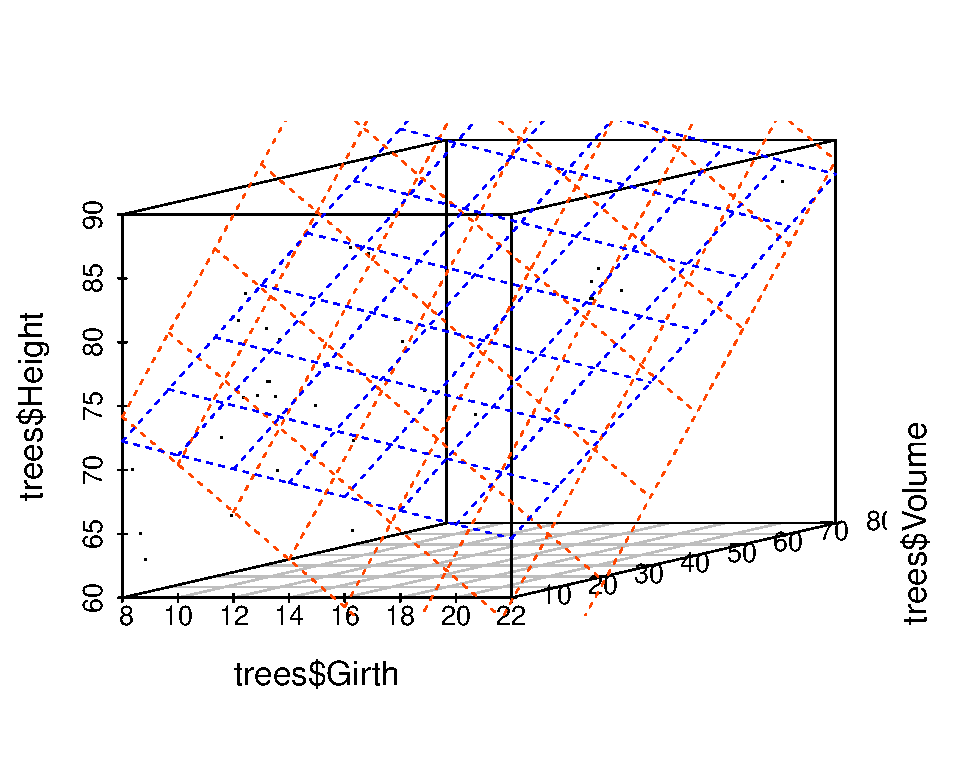
\includegraphics[width=0.5\columnwidth]{./figures/hands-on4/trees-jitterfit-height.pdf}
\caption{Multiple regression plot of cherry tree height on girth and volume, for the original data (red) and the jittered data (blue).\label{fig:jittercompare}}
\end{figure}



Let's do the same comparison for the multiple regression of Volume on Height and Girth.  In this case the predictor variables are \emph{not} nearly collinear.
%
\begin{R}
> lm.V <- lm(Volume ~ Girth + Height, data = trees)
> lm.V.jitter <- lm(Volume ~ Girth + Height, data = jitter.trees)
> coefficients(lm.V)
(Intercept)       Girth      Height 
-57.9876589   4.7081605   0.3392512 
> coefficients(lm.V.jitter)
(Intercept)       Girth      Height 
-51.2670818   4.4798268   0.2906203 
\end{R}
%
For this model, we see that the coefficients have changed only a small amount.  The underlying data, |jitter.trees|, is the same in both cases, but now our model is stable because the predictor variables are only modestly correlated with each other.

Let's generate another plot to illustrate the similarity of the models fit to the original and jittered data when Girth and Height are used to predict Volume. The corresponding output is shown in Fig.~\ref{fig:jittervolume}.
%
\begin{R}
> p <- scatterplot3d(x=trees$Girth, y=trees$Height, z=trees$Volume, 
                     angle=55, type='p', pch='.')
> p$plane3d(lm.V, col='orangered')
> p$plane3d(lm.V.jitter, col='blue')
\end{R}
%
\begin{figure}[htbp]
\centering
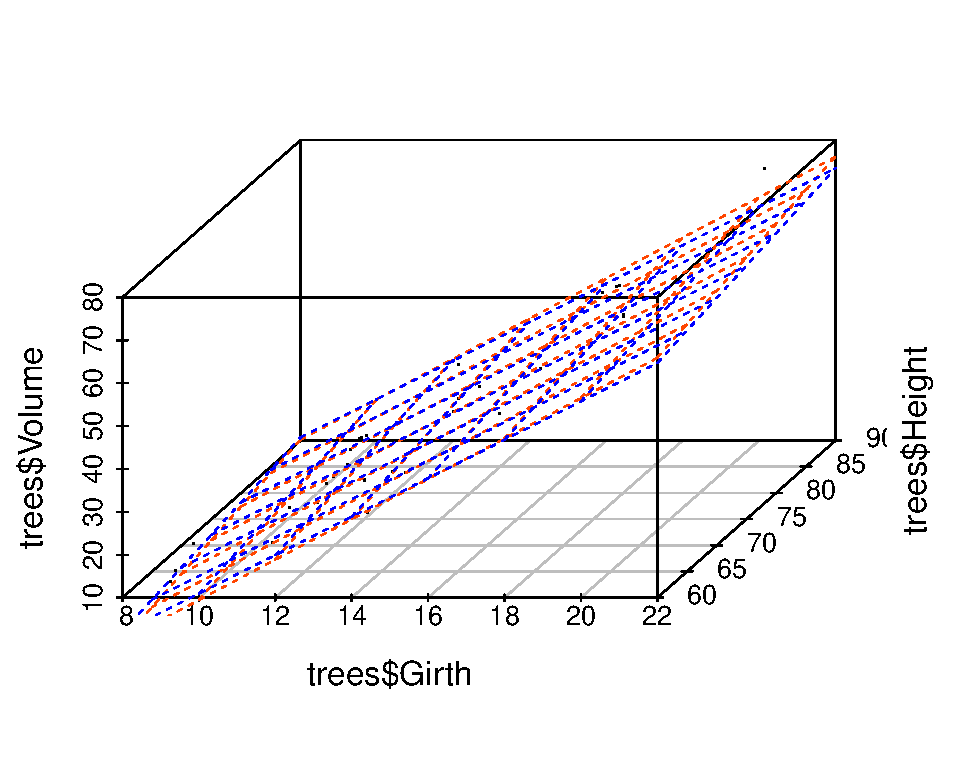
\includegraphics[width=0.5\columnwidth]{./figures/hands-on4/trees-jitterfit-volume.pdf}
\caption{Multiple regression plot of cherry tree volume on girth and height, for the original data (red) and the jittered data (blue).\label{fig:jittervolume}}
\end{figure}

Finally, let's do some vector calculations to quantify how the angular deviation between the fit data and the predictor variables changes between the original and jittered data set for the two different multiple regressions:
%
\begin{R}

# write a quickie fxn to express angle between vectors in degrees
> vec.angle <- function(x,y) { acos(cor(x,y)) * (180/pi)}

# vector angles for fit of Height ~ Girth + Volume (orig)
> vec.angle(lm.H$fitted.values, trees$Girth)
[1] 36.02644
> vec.angle(lm.H$fitted.values, trees$Volume)
[1] 21.29297

# vector angles for fit of Height ~ Girth + Volume (jittered)
> vec.angle(lm.H.jitter$fitted.values, jitter.trees$Girth)
[1] 28.48079
> vec.angle(lm.H.jitter$fitted.values, jitter.trees$Volume)
[1] 9.097828

# CONCLUSION -- angular changes of about 8 and 12 degrees 


# vector angles for fit of Volume ~ Girth + Height (orig)
> vec.angle(lm.V$fitted.values, trees$Girth)
[1] 6.628322
> vec.angle(lm.V$fitted.values, trees$Height)
[1] 52.08771

# vector angles for fit of Volume ~ Girth + Height (jittered)
> vec.angle(lm.V.jitter$fitted.values, jitter.trees$Girth)
[1] 6.163463
> vec.angle(lm.V.jitter$fitted.values, jitter.trees$Height)
[1] 54.33651

# CONCLUSION -- angular changes of about 0.5 and 2 degrees
\end{R}

\section{Manipulating data using split}

Last week we introduced the |reshape()| function from the reshape2 package.  |reshape()| is good for computing simple statistics across multiple `facets' of data. However, more complicated statistics are made possible by using the |split()| function, which is defined in the R base package.

|split()| takes two arguments: 1) a vector or data frame to split and 2) a character vector defining what to split the first argument by. For example, we can split the iris data set by species in order to get a list containing three data frames; one for each species.
%
\begin{R}
> iris.split <- split(iris, iris$Species)
> names(iris.split)
[1] "setosa"     "versicolor" "virginica" 
> str(iris.split)  # see the documentation for the str() function
List of 3
 $ setosa    :'data.frame': 50 obs. of  5 variables:
  ..$ Sepal.Length: num [1:50] 5.1 4.9 4.7 4.6 5 5.4 4.6 5 4.4 4.9 ...
  ..$ Sepal.Width : num [1:50] 3.5 3 3.2 3.1 3.6 3.9 3.4 3.4 2.9 3.1 ...
  ..$ Petal.Length: num [1:50] 1.4 1.4 1.3 1.5 1.4 1.7 1.4 1.5 1.4 1.5 ...
  ..$ Petal.Width : num [1:50] 0.2 0.2 0.2 0.2 0.2 0.4 0.3 0.2 0.2 0.1 ...
  ..$ Species     : Factor w/ 3 levels "setosa","versicolor",..: 1 1 1 1 1 1 1 1 1 1 ...
 $ versicolor:'data.frame': 50 obs. of  5 variables:
  ..$ Sepal.Length: num [1:50] 7 6.4 6.9 5.5 6.5 5.7 6.3 4.9 6.6 5.2 ...
  ..$ Sepal.Width : num [1:50] 3.2 3.2 3.1 2.3 2.8 2.8 3.3 2.4 2.9 2.7 ...
  ..$ Petal.Length: num [1:50] 4.7 4.5 4.9 4 4.6 4.5 4.7 3.3 4.6 3.9 ...
  ..$ Petal.Width : num [1:50] 1.4 1.5 1.5 1.3 1.5 1.3 1.6 1 1.3 1.4 ...
  ..$ Species     : Factor w/ 3 levels "setosa","versicolor",..: 2 2 2 2 2 2 2 2 2 2 ...
 $ virginica :'data.frame': 50 obs. of  5 variables:
  ..$ Sepal.Length: num [1:50] 6.3 5.8 7.1 6.3 6.5 7.6 4.9 7.3 6.7 7.2 ...
  ..$ Sepal.Width : num [1:50] 3.3 2.7 3 2.9 3 3 2.5 2.9 2.5 3.6 ...
  ..$ Petal.Length: num [1:50] 6 5.1 5.9 5.6 5.8 6.6 4.5 6.3 5.8 6.1 ...
  ..$ Petal.Width : num [1:50] 2.5 1.9 2.1 1.8 2.2 2.1 1.7 1.8 1.8 2.5 ...
  ..$ Species     : Factor w/ 3 levels "setosa","versicolor",..: 3 3 3 3 3 3 3 3 3 3 ...
\end{R}

Now that we have a split data frame, it's easy to use |lapply| or |sapply| to calculate complicated summary statistics. For example, this function calculates the mean ratio of |Sepal.Length| to |Petal.Length|:
%
\begin{R}
> ratio.sepal2petal <- function(x) {
+    mean( x$Sepal.Length / x$Petal.Length)
+ }
> sapply(iris.split, ratio.sepal2petal)
    setosa versicolor  virginica 
  3.464906   1.400896   1.188350 
\end{R}
%
We could also write a function to return the coefficients of fitting a linear model to each facet of the data:
%
\begin{R}
> sepal.on.petal.coeff <- function(x){
+       model <- lm(Sepal.Length ~ Petal.Length, data=x)
+       return(model$coeff)
+ }
> sapply(iris.split, sepal.on.petal.coeff)
                setosa versicolor virginica
(Intercept)  4.2131682   2.407523 1.0596591
Petal.Length 0.5422926   0.828281 0.9957386
\end{R}
%
Of course, no analysis would be complete without examining the fit of the linear models. In order to visualize whether the linear model is a good representation of the data, we'll write another function to return a data frame containing the fitted values, residuals, and species names for each element of the list.
%
\begin{R}
> sepal.on.petal.lm.fit <- function(x){
+       model <- lm(Sepal.Length ~ Petal.Length, data=x)
+       data.frame(fitted = fitted(model),
+                  residuals = residuals(model),
+                  species = x$Species)
+ }
> iris.fit <- lapply(iris.split, sepal.on.petal.lm.fit)
> str(iris.fit)
List of 3
 $ setosa    :'data.frame': 50 obs. of  3 variables:
  ..$ fitted   : num [1:50] 4.97 4.97 4.92 5.03 4.97 ...
  ..$ residuals: num [1:50] 0.1276 -0.0724 -0.2181 -0.4266 0.0276 ...
  ..$ species  : Factor w/ 3 levels "setosa","versicolor",..: 1 1 1 1 1 1 1 1 1 1 ...
 $ versicolor:'data.frame': 50 obs. of  3 variables:
  ..$ fitted   : num [1:50] 6.3 6.13 6.47 5.72 6.22 ...
  ..$ residuals: num [1:50] 0.7 0.265 0.434 -0.221 0.282 ...
  ..$ species  : Factor w/ 3 levels "setosa","versicolor",..: 2 2 2 2 2 2 2 2 2 2 ...
 $ virginica :'data.frame': 50 obs. of  3 variables:
  ..$ fitted   : num [1:50] 7.03 6.14 6.93 6.64 6.83 ...
  ..$ residuals: num [1:50] -0.734 -0.338 0.165 -0.336 -0.335 ...
  ..$ species  : Factor w/ 3 levels "setosa","versicolor",..: 3 3 3 3 3 3 3 3 3 3 ...
> 
\end{R}

Next, we'll join the data back into a data frame using the |do.call| and |rbind| functions. Read the documentation to figure out what they do.
%
\begin{R}
> iris.joined <- do.call('rbind', iris.fit)
> str(iris.joined)
'data.frame': 150 obs. of  3 variables:
 $ fitted   : num  4.97 4.97 4.92 5.03 4.97 ...
 $ residuals: num  0.1276 -0.0724 -0.2181 -0.4266 0.0276 ...
 $ species  : Factor w/ 3 levels "setosa","versicolor",..: 1 1 1 1 1 1 1 1 1 1 ...
\end{R}

Finally, we'll visualize our model fits by plotting our data using ggplot:
%
\begin{R}
> library(ggplot2)
> ggplot(iris.joined, aes(x=fitted, y=residuals))+
+   geom_point()+
+   facet_wrap(~species, scale='free') + 
+   ggtitle("Residuals from Regression of \nSepal Length on Petal Length for 3 Iris Species")
\end{R}
Examining the residuals (Fig.~\ref{fig:irissplit}), we see they look fairly uniform across the range of fit values. The term that statiscians use for this is `homoscedastic'; when the residuals are non uniform we say they are `heteroscadistic'.
%
\begin{figure}[htbp]
\centering
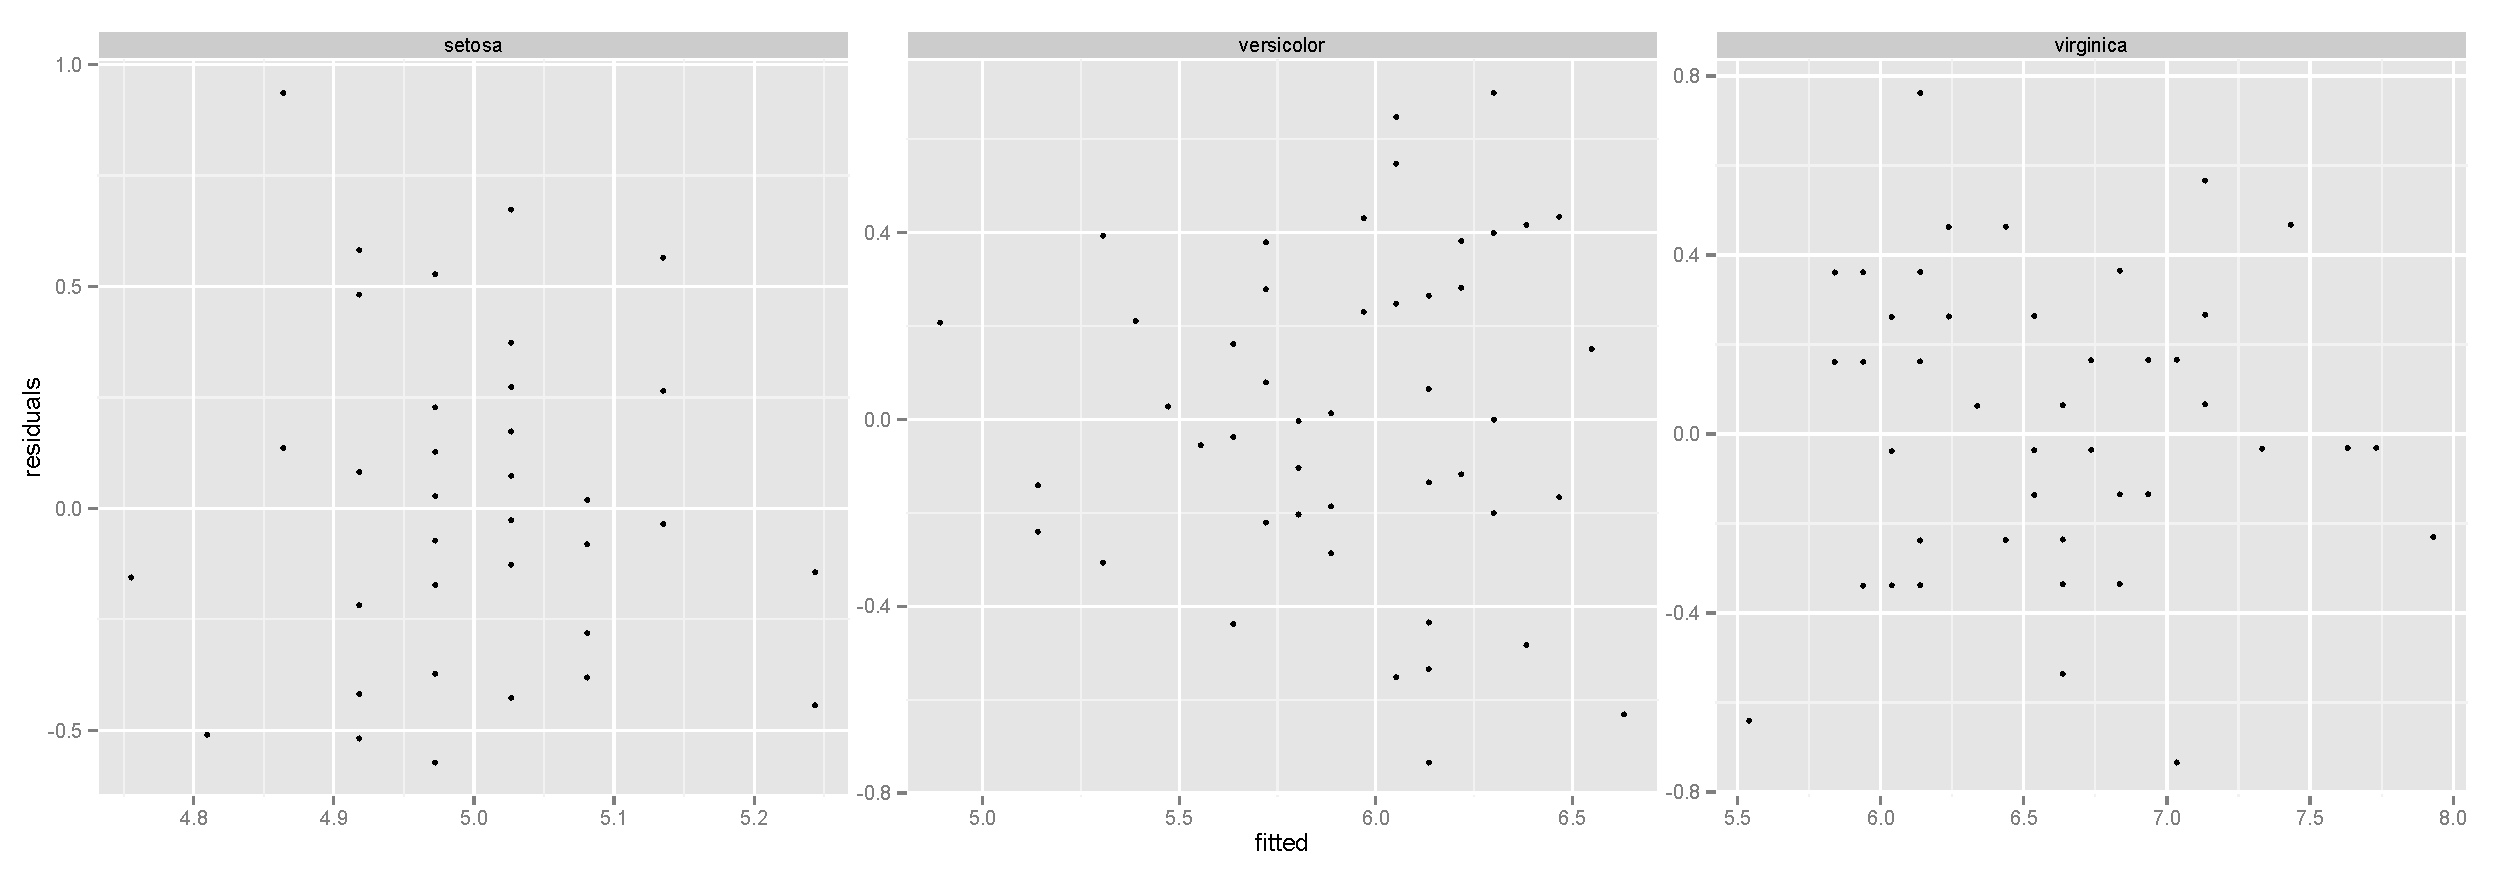
\includegraphics[width=0.75\columnwidth]{./figures/hands-on4/iris-residuals.pdf}
\caption{Residuals from regressions of Sepal Length on Petal Length, for the Iris data set split by species.\label{fig:irissplit}}
\end{figure}


An alternate way to visualize the fits, without the benefit of  getting the info on the model fits back for further examination, is to use the |stat_smooth()| to plot a linear fit of our data for each facet (Fig.~\ref{fig:irisregressions}). Read the |stat_smooth| documentation to how this works.
%
\begin{R}
> ggplot( iris, aes(x=Petal.Length, y=Sepal.Length))+
   geom_point()+
   stat_smooth(method="lm")+
   facet_wrap(~Species, scale='free')+
   ggtitle("Regressions of Sepal Length on Petal Length")
\end{R}
%
\begin{figure}[htbp]
\centering
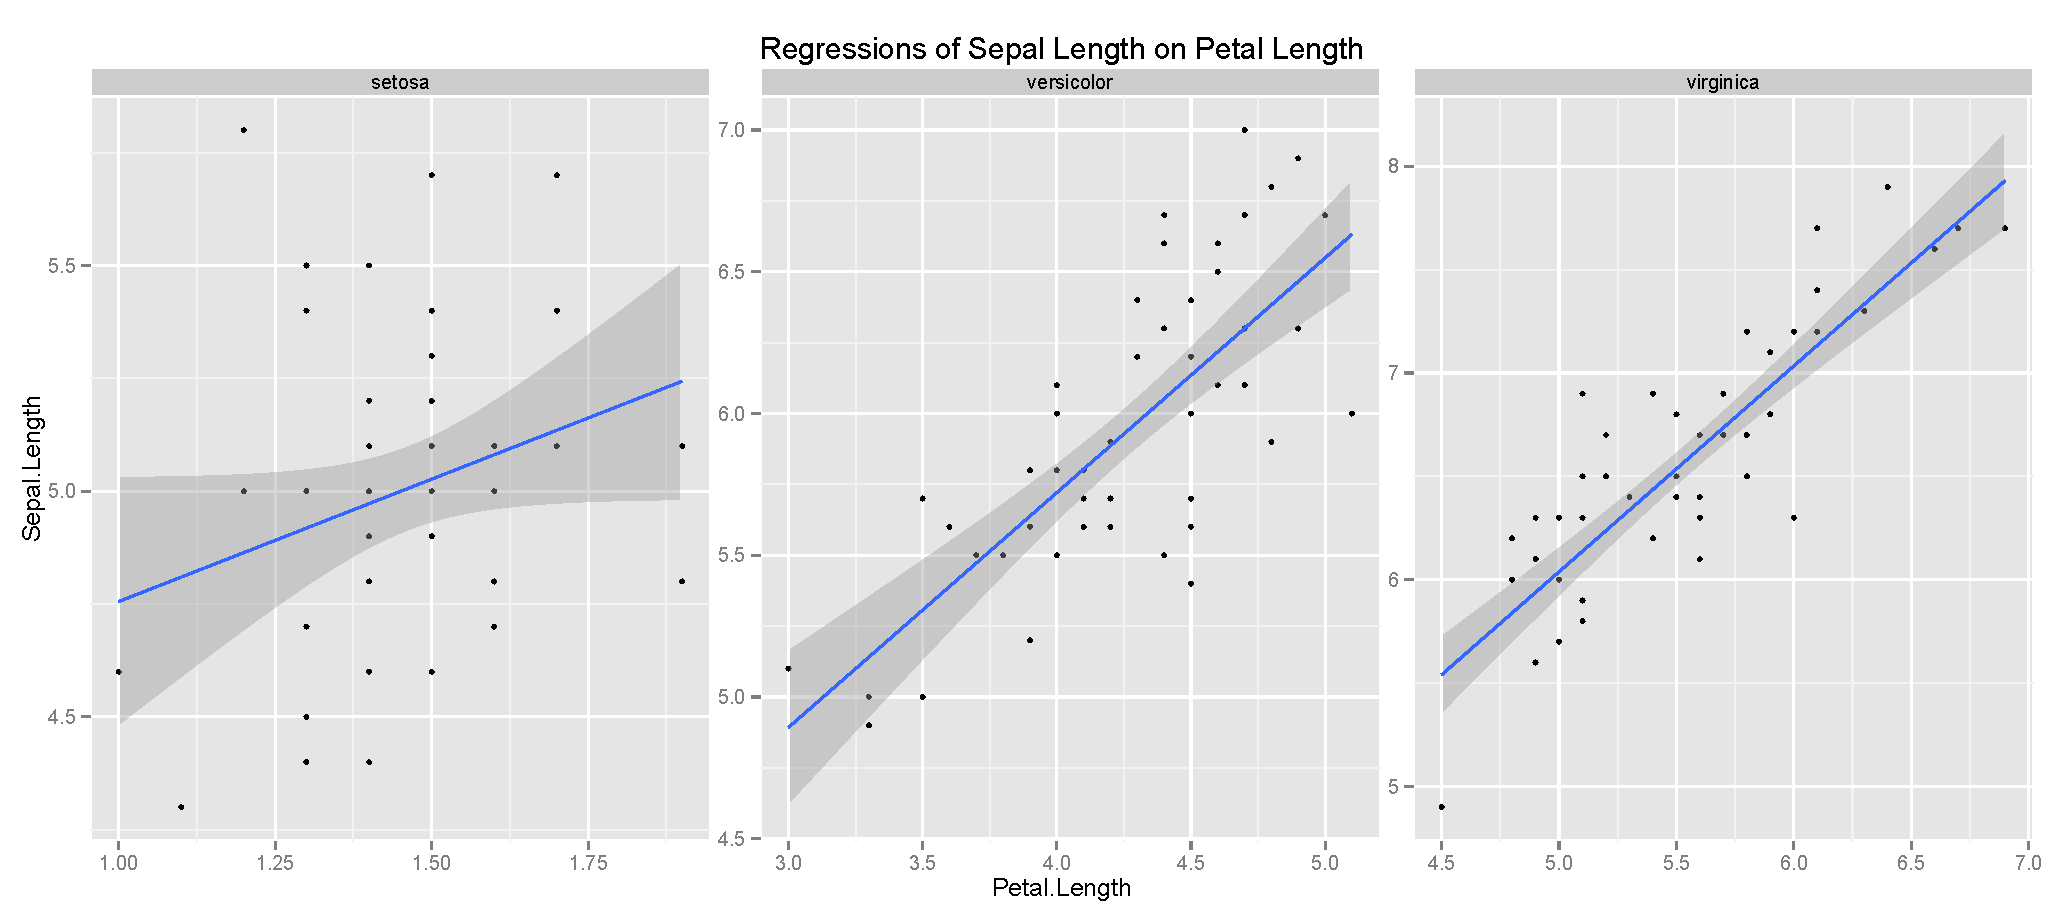
\includegraphics[width=0.75\columnwidth]{./figures/hands-on4/iris-regressions.pdf}
\caption{Regressions of Sepal Length on Petal Length, for the Iris data, produced using the \lstinline|stat_smooth()| function in ggplot2.\label{fig:irisregressions}}
\end{figure}
%


% \chapter{Eigenanalysis and PCA in R}
% 
\section{Eigenanalysis in R}

The \lstinline!eigen()! function computes the eigenvalues and
eigenvectors of a square matrix.

\begin{R}
> A <- matrix(c(2,1,2,3),nrow=2)
> A
     [,1] [,2]
[1,]    2    2
[2,]    1    3
> eigen.A <- eigen(A)
> eigen.A
$values
[1] 4 1
$vectors
           [,1]       [,2]
[1,] -0.7071068 -0.8944272
[2,] -0.7071068  0.4472136
> V <- eigen.A$vectors
> D <- diag(eigen.A$values) # diagonal matrix of eigenvalues
> Vinv <- solve(V)
> V %*% D %*% Vinv  # reconstruct our original matrix (see lecture slides)
     [,1] [,2]
[1,]    2    2
[2,]    1    3
> Vinv %*% A %*% V
             [,1] [,2]
[1,] 4.000000e+00    0
[2,] 2.220446e-16    1
> all.equal(Vinv %*% A %*% V, D) # test 'near equality'
[1] TRUE
> V[,1] %*% V[,2] # note that the eigenvectors are NOT orthogonal. Why?
          [,1]
[1,] 0.3162278
> B <- matrix(c(2,2,2,3),nrow=2) # define another tranformation
> B
     [,1] [,2]
[1,]    2    2
[2,]    2    3
> eigen.B$values
[1] 4.5615528 0.4384472
> eigen.B$vectors
          [,1]       [,2]
[1,] 0.6154122 -0.7882054
[2,] 0.7882054  0.6154122
> Vb <- eigen.B$vectors
> Vb[,1] %*% Vb[,2] # these eigenvectors ARE orthogonal.
     [,1]
[1,]    0
\end{R}
As we discussed in lecture, the eigenvectors of a square matrix,
$\mathbf{A}$, point in the directions that are unchanged by the
transformation specified by $\mathbf{A}$. The following relationships
relate $\mathbf{A}$ to it's eigenvectors and eigenvalues:

\[\mathbf{V}^{-1}\mathbf{A}\mathbf{V}  =  \mathbf{D} \]

\[\mathbf{A}  =  \mathbf{V}\mathbf{D}\mathbf{V}^{-1}\]
%
where $\mathbf{V}$ is a matrix where the columns represent the eigenvectors, and $\mathbf{D}$ is a diagonal matrix of eigenvalues.

Since $A$ and $B$ represent 2D transformations we can visualize the
effect of these transformations using points in the plane. We'll show
how they distort a set of points that make up a square.

\begin{R}
# define the corners of a square
> pts <- matrix(c(1,1, 1,-1, -1,-1, -1,1),4,2,byrow=T)
> pts
     [,1] [,2]
[1,]    1    1
[2,]    1   -1
[3,]   -1   -1
[4,]   -1    1
> plot(pts,xlim=c(-6,6),ylim=c(-6,6),asp=1) # plot the corners
> polygon(pts) # draw edges of square
> transA <- A %*% t(pts)
> transA
     [,1] [,2] [,3] [,4]
[1,]    4    0   -4    0
[2,]    4   -2   -4    2
> newA <- t(transA)
> newA
     [,1] [,2]
[1,]    4    4
[2,]    0   -2
[3,]   -4   -4
[4,]    0    2
> points(newA, col='red') # plot the A transformation
> polygon(newA, lty='dashed', border='red')
> newB <- t(B %*% t(pts)) # do the same for the B transformation
> polygon(newB, lty='dashed', border='blue')
> points(newB, col='blue')
> legend("topleft", c("transformation A","transformation B"),
lty=c("dashed","dashed"),col=c("red","blue"))
\end{R}
The code given above will produce the plot show in the figure below.

\begin{figure}[htbp]
\centering
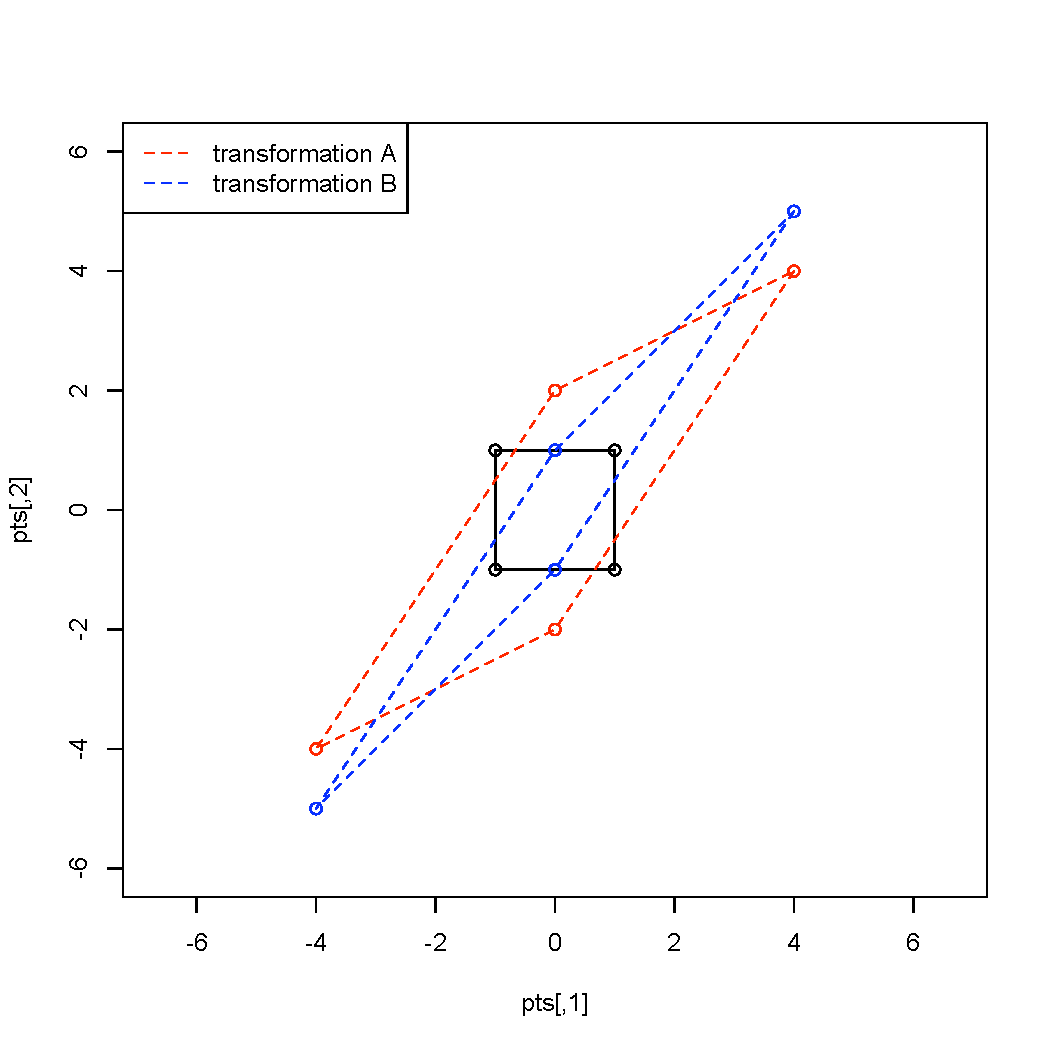
\includegraphics[width=2in]{./figures/hands-on5/eigen-transform.pdf}
\caption{Transformation of a square represented by two matrices, A and
B}
\end{figure}

\begin{assignment}
Fig.~\ref{fig:eigen} illustrates the geometry of the eigenvectors for matrices A and B as defined above.  Note that the lengths of the eigenvector depictions are scaled to be proportional to their eigenvalues. Write R code to reconstruct this figure.

\medskip

\textbf{Extra Credit:} For extra credit, write a function called |draw_eigenvector()| that will create a similar figure for any arbitrary matrix that represents a 2D transformation. Your function should tak as input a matrix $\mathbf{A}$, and a set of points in the plane.  Make sure to include code to handle cases where $\mathbf{A}$ is singular.
\end{assignment}

\begin{figure}[htbp]
\centering
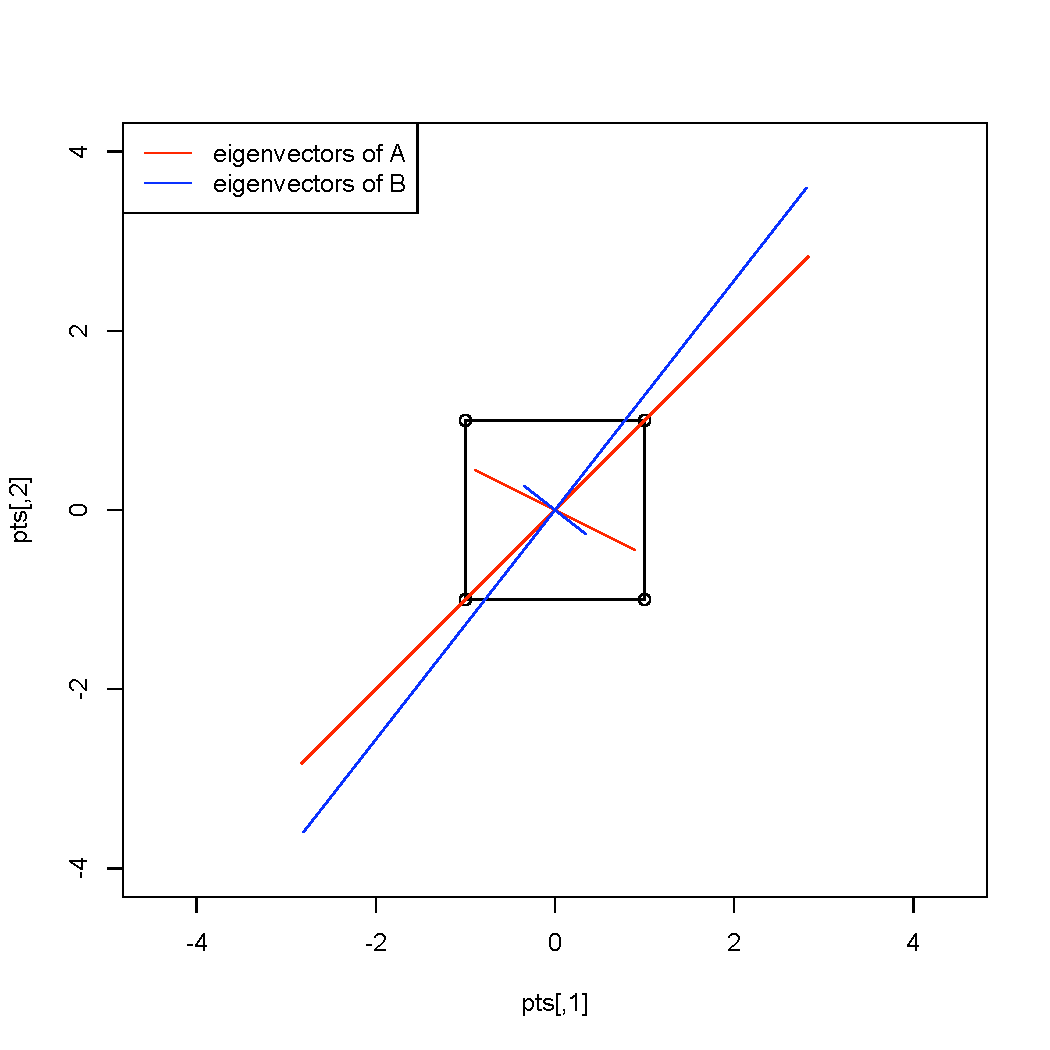
\includegraphics[width=2in]{./figures/hands-on5/eigen-ECplot.pdf}
\caption{Eigenvectors of matrices A and B \label{fig:eigen}}
\end{figure}
%
\section{Eigenanalysis in Python}

The eigenanalysis functions in Python are found in the
\lstinline!linalg! module in the \lstinline!Numpy! package. These
functions are specified by \lstinline!linalg.eig()! (which returns both
eigenvalues and eigenvectors) and \lstinline!linalg.eigvals()! (which
only returns the eigenvalues).

\begin{python}
>>> import numpy as np, numpy.linalg as la
>>> A = np.array([[2,2],[1,3]],np.float)
>>> A
array([[ 2.,  2.],
       [ 1.,  3.]])
>>> evals, evecs = la.eig(A)
>>> evals
array([ 1.,  4.])
>>> evecs
array([[-0.89442719, -0.70710678],
       [ 0.4472136 , -0.70710678]])
\end{python}
Note that (somewhat inconveniently) the \lstinline!eig()! function does
not necessarily return the eigenvalues and eigenvectors in sorted
fashion. The Numpy documentation states that the normalized eigenvector
corresponding to the eigenvalue \lstinline!w[i]! is the column
\lstinline!v[:,i]!. Also note that both the R \lstinline!eigen()!
function and the Numpy \lstinline!eig()! function return normalized
eigenvectors (i.e.~each eigenvector has length 1).

We can get sort the eigenvectors by their eigenvalues as so:

\begin{python}
>>> colorder = list(np.argsort(evals)) # get back argsort as a list
>>> colorder
[0, 1]
>>> colorder.reverse() # need to reverse the column order because want from large to small
>>> colorder
[1, 0]
>>> srtevals = np.take(evals, colorder) #see the Numpy docs on take()
>>> srtevals
array([ 4.,  1.])
>>> srtevecs = np.take(evecs, colorder,axis=1) # sort columns
>>> srtevecs
array([[-0.70710678, -0.89442719],
       [-0.70710678,  0.4472136 ]])
>>> V = srtevecs
>>> Vinv = la.inv(srtevecs)
>>> D = np.diag(srtevals)
>>> np.dot(V, np.dot(D, Vinv))
array([[ 2.,  2.],
       [ 1.,  3.]])
>>> Arecon = np.dot(V, np.dot(D, Vinv))
>>> Arecon == A
array([[ True,  True],
       [ True, False]], dtype=bool)
>>> np.allclose(Arecon, A)  # like R's all.equal()
True     
\end{python}
See the Numpy docs for more information on the \lstinline!argsort()!
(\href{http://docs.scipy.org/doc/numpy/reference/routines.sort.html}{Numpy:
Sorting and searching}), \lstinline!take()!
((\href{http://docs.scipy.org/doc/numpy/reference/routines.indexing.html}{Numpy:
Indexing Routines}), and \lstinline!allclose()!
(\href{http://docs.scipy.org/doc/numpy/reference/routines.logic.html}{Numpy:
Logic functions}).

\begin{assignment}
Write a Python function that takes as input a
square matrix, and returns a vector of sorted eigenvalues (sorted from
largest to smallest) and the corresponding matrix of eigenvectors sorted
according to their corresponding eigenvalues.
\end{assignment}

\section{Principal Components Analysis in R}

There are two functions in R for carrying out PCA - \lstinline!princomp()! and
\lstinline!prcomp()!. The \lstinline!princomp()! function uses the
\lstinline!eigen()! function to carry out the analysis on the covariance
matrix or correlation matrix, while \lstinline!prcomp()! carries out an
equivalent analysis, starting from a data matrix, using a technique called
singular value decomposition (SVD). The SVD routine has greater numerical
accuracy, so the |prcomp()| function should generally be preferred. The
\lstinline!princomp()! function is also useful when you don't have access to
the original data, but you do have a covariance or correlation matrix (a
frequent situation when re-analyzing data from the literature). We'll concentrate on using the |prcomp()| function.


\subsection{Bioenv dataset}
To demonstrate PCA we'll use a dataset called `bioenv.txt' (see class wiki), obtained from a book called ``Biplots in Practice'' (M. Greenacre, 2010). Here is Greenacre's description of the dataset:

\begin{quote}
  The context is in marine biology and the data consist of two sets of variables observed at the same locations on the sea-bed: the first is a set of biological variables, the counts of five groups of species, and the second is a set of four environmental variables. The data set, called ``bioenv'', is shown in Exhibit 2.1. The species groups are abbreviated as ``a'' to ``e''. The environmental variables are ``pollution'', a composite index of pollution combining measurements of heavy metal concentrations and hydrocarbons; depth, the depth in metres of the sea-bed where the sample was taken; ``temperature'', the temperature of the water at the sampling point; and ``sediment'', a classification of the substrate of the sample into one of three sediment categories.
\end{quote}

The first column has no header, and corresponds to the site labels.
%
\begin{R}
> b <- read.delim('bioenv.txt',row.names=1) # note use of row.names argument
[1] "a"           "b"           "c"           "d"           "e"
[6] "Pollution"   "Depth"       "Temperature" "Sediment"
\end{R}

The columns labeled `a' to `e' contain the counts of the five species at each site.  We'll work with this abundance data for now.
%
\begin{R}
> abund <- subset(b, select=c(a,b,c,d,e))
> boxplot(abund, xlab="Species", ylab="Counts", main="Distribution of\nSpecies Counts per Site")
\end{R}

From the boxplot it looks like the counts for species `e' are smaller on average, and less variable. The mean and variance functions confirm that.
%
\begin{R}
> apply(abund,2,mean)
        a         b         c         d         e
13.466667  8.733333  8.400000 10.900000  2.966667
> apply(abund,2,var)
        a         b         c         d         e
157.63678  83.44368  73.62759  44.43793  15.68851
\end{R}


A correlation matrix suggests weak to moderate associations between the variables, but the scatterplot matrix generated by the |chart.Correlation()| function suggests that many of the relationships have a strong non-linear element.
%
\begin{R}
> cor(abund)
           a           b           c            d            e
a  1.0000000  0.67339954 -0.23992888  0.358192050  0.273522301
b  0.6733995  1.00000000 -0.08041947  0.501834036  0.036914702
c -0.2399289 -0.08041947  1.00000000  0.081504483 -0.343540453
d  0.3581921  0.50183404  0.08150448  1.000000000 -0.004048517
e  0.2735223  0.03691470 -0.34354045 -0.004048517  1.000000000

> library(PerformanceAnalytics)
> chart.Correlation(abund)
\end{R}

\subsection{PCA of the Bioenv dataset}
Linearity is not a requirement for PCA, as it's simply a rigid rotation of the original data. So we'll continue with our analysis after taking a moment to read the help on the |prcomp()| function.
\begin{R}
> ?prcomp
> a.pca <- prcomp(abund, center=T, retx=T)
    # center=T mean centers the data
    # retx=T returns the PC scores
    # if you want to do PCA on correlation matrix set scale.=T
    #    -- notice the period after scale!

> summary(a.pca)
Importance of components:
                           PC1    PC2    PC3     PC4     PC5
Standard deviation     14.8653 8.8149 6.2193 5.03477 3.48231
Proportion of Variance  0.5895 0.2073 0.1032 0.06763 0.03235
Cumulative Proportion   0.5895 0.7968 0.9000 0.96765 1.00000
\end{R}
We see that approximately 59\% of the variance in the data is capture by the first PC, and approximately 90\% by the first three PCs.

Let's compare the values return by PCA to what we would get if we carried out eigenanalysis of the covariance matrix that corresponds to our data.

\begin{R}
> a.pca
Standard deviations:
[1] 14.865306  8.814912  6.219250  5.034774  3.482308

Rotation:
          PC1         PC2         PC3         PC4         PC5
a  0.81064462  0.07052882 -0.53108427  0.18442140 -0.14771336
b  0.51264394 -0.27799671  0.47711910 -0.63418946  0.17342177
c -0.16235135 -0.88665551 -0.40897655 -0.01149647  0.14173943
d  0.22207108 -0.31665237  0.56250980  0.72941223 -0.04422938
e  0.06616623  0.17696554 -0.08141111  0.17781482  0.96231977
> eigen(cov(abund))
$values
[1] 220.97732  77.70266  38.67908  25.34895  12.12647

$vectors
            [,1]        [,2]        [,3]        [,4]        [,5]
[1,]  0.81064462 -0.07052882  0.53108427  0.18442140 -0.14771336
[2,]  0.51264394  0.27799671 -0.47711910 -0.63418946  0.17342177
[3,] -0.16235135  0.88665551  0.40897655 -0.01149647  0.14173943
[4,]  0.22207108  0.31665237 -0.56250980  0.72941223 -0.04422938
[5,]  0.06616623 -0.17696554  0.08141111  0.17781482  0.96231977
\end{R}
Notice that the `rotation' object returned by the |prcomp| function are the scaled eigenvectors (scaled to have length 1). The standard deviations of the PCA are the square roots of the eigenvalues of the covariance matrix.

\subsection{Calculating Factor Loadings}

Let's calculate the `factor loadings' associated with the PCs:
\begin{R}
> V <- a.pca$rotation # eigenvectors
> L <- diag(a.pca$sdev) # diag mtx w/sqrt of eigenvalues on diag.

> a.loadings <- V %*% L
> a.loadings
        [,1]       [,2]       [,3]        [,4]       [,5]
a 12.0504801  0.6217053 -3.3029460  0.92852016 -0.5143835
b  7.6206090 -2.4505164  2.9673232 -3.19300085  0.6039081
c -2.4134024 -7.8157898 -2.5435276 -0.05788214  0.4935804
d  3.3011545 -2.7912626  3.4983893  3.67242602 -0.1540203
e  0.9835813  1.5599356 -0.5063161  0.89525751  3.3510942
\end{R}
The magnitude of the loadings is what you want to focus on. For example, species `a' and `b' contribute most to the first PC, while species `c' has the largest influence on PC2.

You can think of the loadings, as defined above, as the components (i.e lengths of the projected vectors) of the original variables with respect to the PC basis vectors.  Since vector length is proportional to the standard deviation of the variables they represent, you can think of the loadings as giving the standard deviation of the original variables with respect the PC axes. This implies that the loadings squared sum to the total variance in the original data, as illustrated below.
\begin{R}
> apply(a.loadings**2, 1, sum)
        a         b         c         d         e
157.63678  83.44368  73.62759  44.43793  15.68851
> apply(abund, 2, var)
        a         b         c         d         e
157.63678  83.44368  73.62759  44.43793  15.68851
\end{R}

\subsection{Drawing Figures to Represent PCA}

\subsubsection{PC Score Plots}

The simplest PCA figure is to depict the PC scores, i.e. the projection of the observations into the space defined by the PC axes. Let's make a figure with three subplots, depicting PC1 vs PC2, PC1 vs PC3, and PC2 vs. PC3.
\begin{R}
> par(mfrow=c(1,3))
> plot(a.pca$x[,1], a.pca$x[,2],asp=1,pch=16, xlab='PC1', ylab='PC2',xlim=c(-30,30),ylim=c(-30,30))
> plot(a.pca$x[,1], a.pca$x[,3],asp=1,pch=16, xlab='PC1', ylab='PC3',xlim=c(-30,30),ylim=c(-30,30))
> plot(a.pca$x[,2], a.pca$x[,3],asp=1,pch=16, xlab='PC2', ylab='PC3',xlim=c(-30,30),ylim=c(-30,30))
\end{R}
Note that you should always set |asp=1| when plotting PC scores, so that the distances between points are accurate representations. Note too that I used the |xlim| and |ylim| arguments to keep the axis limits the same in all plots; comparable scaling of axes is important when comparing plots. Also note the use of the |mfrow| argument to |par()| in order to setup a multicolumn plot.

\begin{figure}[htbp]
\centering
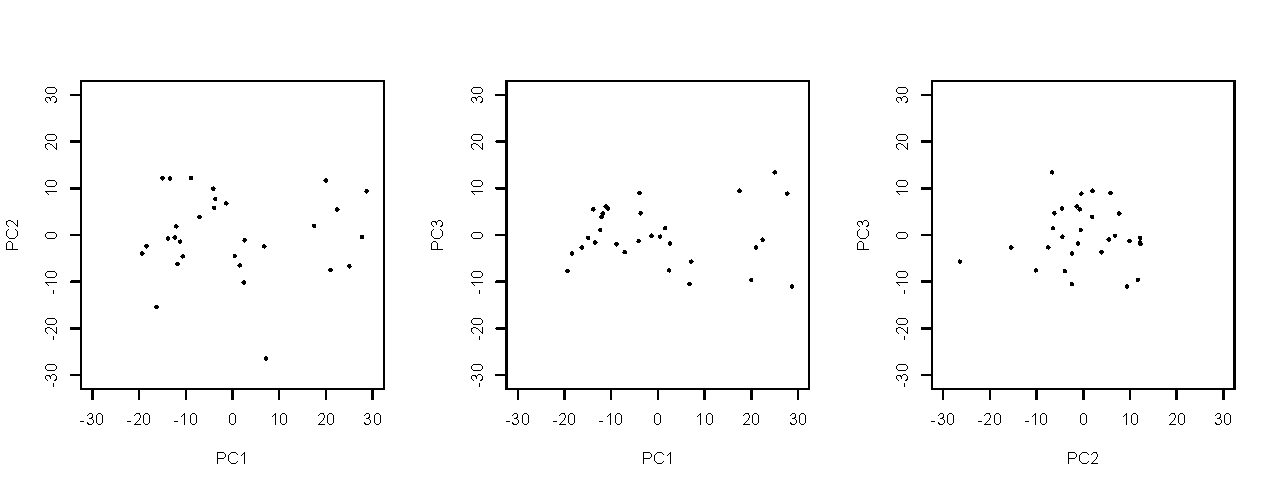
\includegraphics[width=0.95\columnwidth]{./figures/hands-on5/bioenv-scores.pdf}
\caption{Projection of the bioenv dataset into the basis defined by the first three PCs.}\label{fig:bioenvscore}
\end{figure}


As we did in previous weeks we can also use one of the 3D plotting functions to make a 3D scatterplot of the scores.
\begin{R}
> library(rgl)
> plot3d(a.pca$x[,1:3], asp=1, type='s', xlim=c(-30,30), ylim=c(-30,30), zlim=c(-30,30),col='red',size=2)
\end{R}

\subsubsection{Simultaneous Depiction of Observations and Variables in the PC Space}

Let's return to our simple PC score plot.  As we discussed above, the loadings are components of the original variables in the space of the PCs. This implies we can depict those loadings in the same PC basis that we use to depict the scores.
%
\begin{R}
> plot(a.pca$x[,1], a.pca$x[,2],asp=1,pch=16, xlab='PC1', ylab='PC2',xlim=c(-30,30),ylim=c(-30,30))

# get the loadings for each variable w/respect to PCs 1 and 2
> load2d.a <- a.loadings[1,1:2]
> load2d.b <- a.loadings[2,1:2]
> load2d.c <- a.loadings[3,1:2]
> load2d.d <- a.loadings[4,1:2]
> load2d.e <- a.loadings[5,1:2]

# draw arrows depicting loadings
> arrows(0, 0, load2d.a[1], load2d.a[2], length=0.1, col='red')
> text(load2d.a[1], load2d.a[2], 'a',col='red')
> arrows(0, 0, load2d.b[1], load2d.b[2], length=0.1, col='red')
> text(load2d.b[1], load2d.b[2], 'b',col='red')
> arrows(0, 0, load2d.c[1], load2d.c[2], length=0.1, col='red')
> text(load2d.c[1], load2d.c[2], 'c',col='red')
> arrows(0, 0, load2d.d[1], load2d.d[2], length=0.1, col='red')
> text(load2d.d[1], load2d.d[2], 'd',col='red')
> arrows(0, 0, load2d.e[1], load2d.e[2], length=0.1, col='red')
> text(load2d.e[1], load2d.e[2], 'e',col='red')
\end{R}
%
\begin{figure}[htbp]
\centering
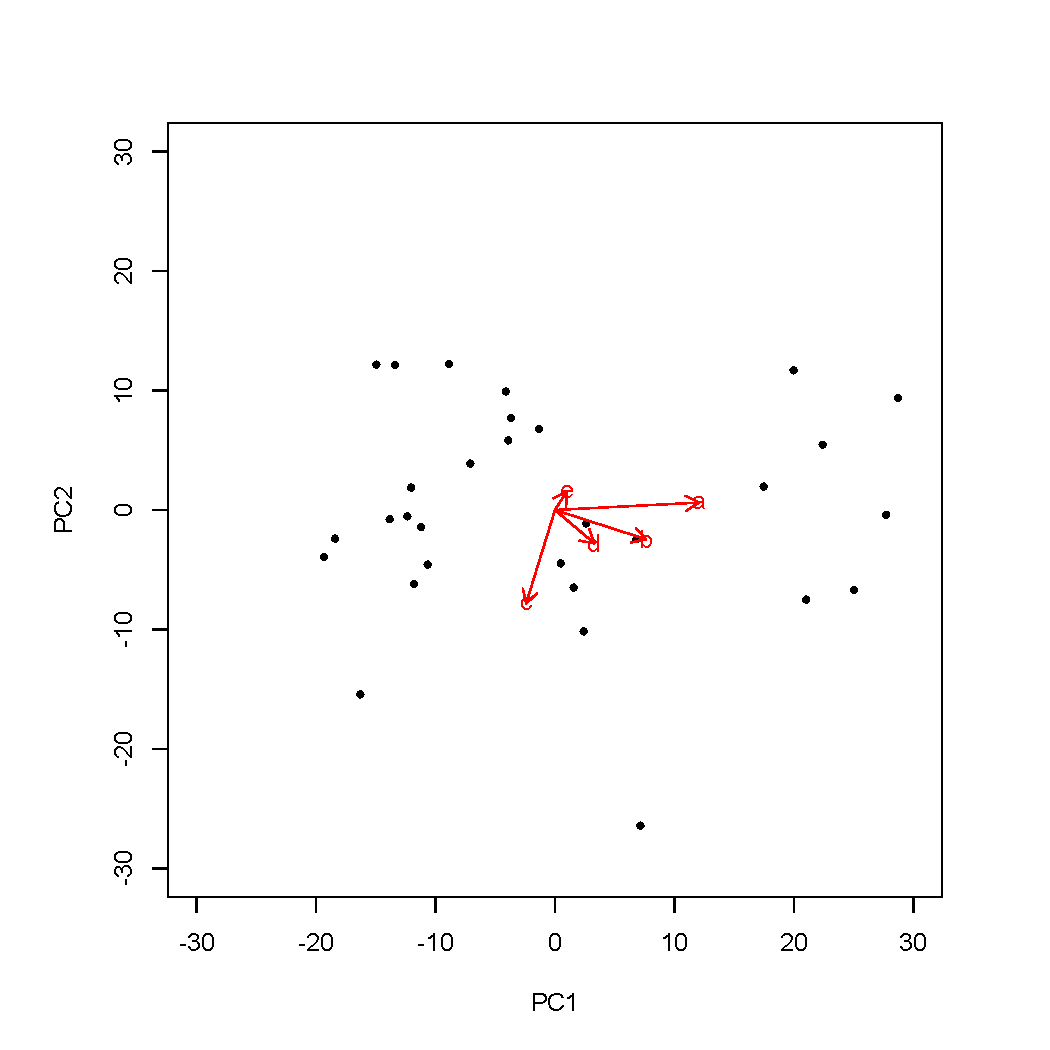
\includegraphics[width=0.5\columnwidth]{./figures/hands-on5/bioenv-simplebiplot.pdf}
\caption{PCA of the bioenv dataset. This biplot represents both the observations (black points) and variables (red vectors) in the space of PCs 1 and 2.}\label{fig:bioenvbiplot}
\end{figure}

The output of the code above should look  like Fig.~\ref{fig:bioenvbiplot}. Fig.~\ref{fig:bioenvbiplot} is called a `biplot', as it simultaneously depicts both the observations and variables in the same space.  From this biplot we can immediately see that variable `a' is highly correlated with PC1, but only weakly associated with PC2. Conversely, variable `c' is strongly correlated with PC2 but only weakly so with PC1. We can also approximate the correlations among the variables themselves -- for example `b' and `d' are fairly strongly correlated, but weakly correlated with `c'.  Keep in mind however that with respect to the relationships among the variables, this visualization is a 2D projection of a 5D space so the geometry is approximate.

The biplot is a generally useful tool for multivariate analyses and there are a number of different ways to define biplots. We'll study biplots more formally in a few weeks after we've covered singular value decomposition.



\bigskip

\begin{assignment}
Do a PCA analysis on the iris data set with all
three species pooled together. Generate a plot showing the projection of
the specimens on the first two PC axes as shown in \cref{fig:pca}.
Represent the specimens from a given species with different colors. Make
sure you include a legend for your plot.
\end{assignment}

\begin{figure}[htbp]
\centering
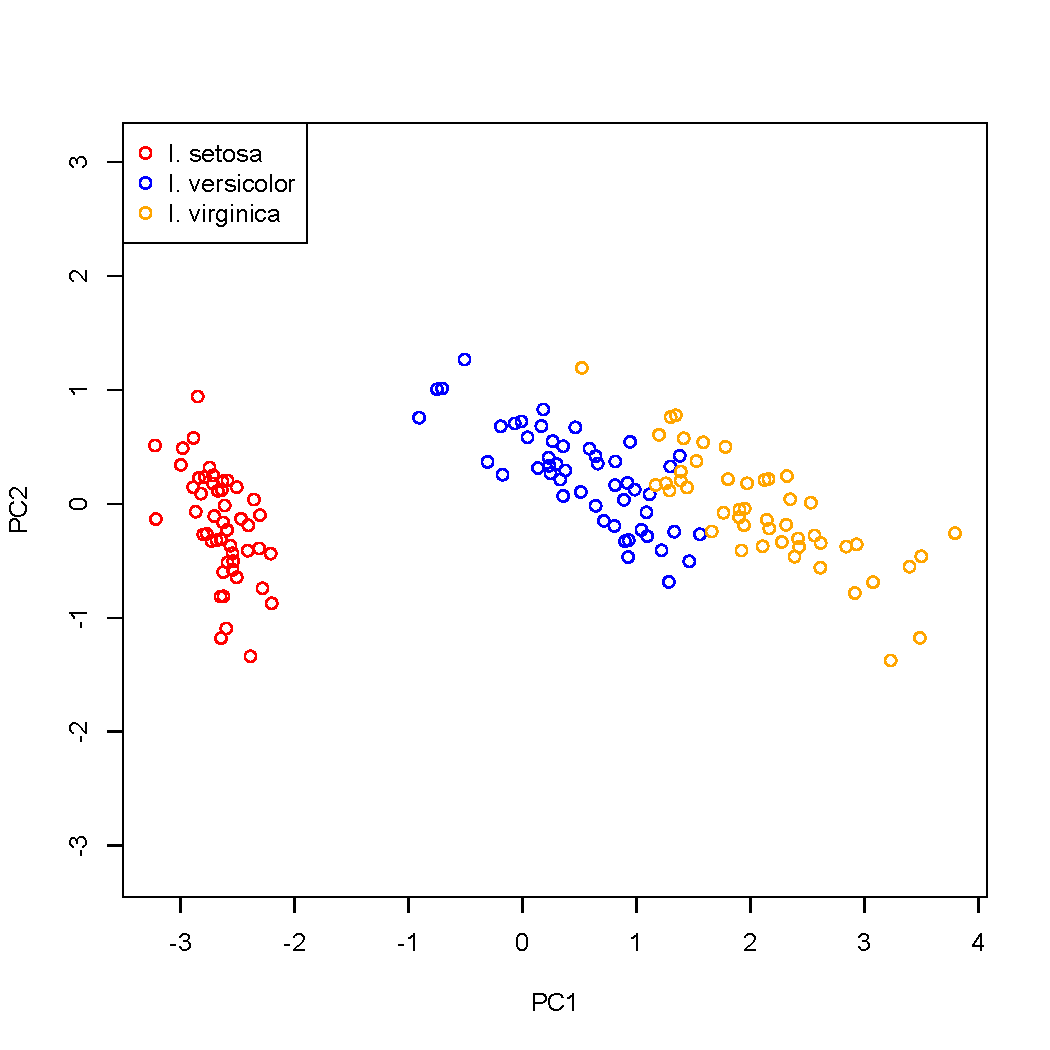
\includegraphics[width=0.5\columnwidth]{./figures/hands-on5/iris-all-pca.pdf}
\caption{PCA of the iris data set. One of your assignments is to
reconstruct this figure on your own.}\label{fig:pca}
\end{figure}


%\section{Principal Components Analysis in Python}

There are no built-in functions for carrying out PCA in Python. Luckily
you have all the tools you need at your disposal to write your own PCA
module.

Note that when performing PCA on a correlation matrix, to get the proper
PC scores you need to use mean centered and standardized variates.

Here's an example:

\begin{python}
>>> import numpy as np, numpy.linalg as la
>>> turt = np.loadtxt('turtles.txt',skiprows=1,usecols=(1,2,3)) # see the Numpy docs
>>> turt.shape
(48, 3)
>>> import pylab # convenient interface to Matplotlib
>>> pylab.scatter(turt[:,0], turt[:,1])
<matplotlib.collections.CircleCollection object at 0x2502630>
>>> pylab.show()
>>> pylab.scatter(turt[:,0], turt[:,2])
<matplotlib.collections.CircleCollection object at 0x66d4a30>
>>> pylab.scatter(turt[:,1], turt[:,2])
<matplotlib.collections.CircleCollection object at 0x63296b0>
>>> tmean = np.mean(turt,axis=0) # get the column means
>>> tmean
array([ 124.6875    ,   95.4375    ,   46.33333333])
>>> deviates = turt - tmean # this mean centers each observation
>>> stdized = deviates/np.std(deviates,axis=0) # standardize variates
>>> pylab.scatter(stdized[:,0],stdized[:,1],color='red') # plot the standardized observations
>>> tcor = np.corrcoef(turt,rowvar=False)
>>> tcor
array([[ 1.        ,  0.97831162,  0.96469455],
       [ 0.97831162,  1.        ,  0.96057053],
       [ 0.96469455,  0.96057053,  1.        ]])
>>> u,v = la.eig(tcor)
>>> u # the eigenvalues
array([ 2.93573765,  0.02141848,  0.04284387])
>>> v  
array([[-0.57879812, -0.74789704, -0.32502731],
       [-0.57798399,  0.65741263, -0.48346989],
       [-0.57526276,  0.09197088,  0.81278171]])
>>> colsort = np.argsort(u)[::-1] # fancy way  to do the 
                  # argsort and reversing to sort index in one call
>>> colsort
array([0, 2, 1])
>>> usort = np.take(u,colsort)
>>> vsort = np.take(v,colsort,axis=1)
>>> usort
array([ 2.93573765,  0.04284387,  0.02141848])
>>> vsort # the PC coefficents are the normalized eigenvectors
array([[-0.57879812, -0.32502731, -0.74789704],
       [-0.57798399, -0.48346989,  0.65741263],
       [-0.57526276,  0.81278171,  0.09197088]])
>>> L = np.diag(usort**0.5) # mtx with sqrt of eigenvalues on diagonal
>>> L
array([[ 1.71339944,  0.        ,  0.        ],
       [ 0.        ,  0.2069876 ,  0.        ],
       [ 0.        ,  0.        ,  0.14635054]])
>>> f=np.dot(vsort,L) # "factor loadings" -- gives corr. btw original vars and PC axes
>>> f
array([[-0.99171237, -0.06727662, -0.10945514],
       [-0.99031745, -0.10007227,  0.09621269],
       [-0.98565489,  0.16823574,  0.01345999]])
>>> scores = np.dot(stdized,vsort)
>>> scores[:5]  # compare to the values you got in R
array([[ 2.00466025,  0.16892135,  0.13583391],
       [ 1.72362844, -0.02689852,  0.10856089],
       [ 1.35439901,  0.2874806 ,  0.25768234],
       [ 1.43581697,  0.05967203,  0.16172995],
       [ 0.95235368,  0.30990249,  0.16324351]])
>>> pylab.scatter(scores[:,0],scores[:,1]) # don't close the plot 
                                        # or else the next line won't work
<matplotlib.collections.CircleCollection object at 0x66d5f50>
>>> pylab.axes().set_aspect(1) # equivalent of the asp=1 argument in R
>>> pylab.xlim(-5,3)  # to make the plot limits more like those we saw in R
(-5, 3)
>>> pylab.ylim(-3,3)
(-3, 3)
\end{python}

\begin{assignment}
Write a Python function that takes as it's input
an $n \times p$ data matrix and returns the following four objects
(\emph{in this order}):

\begin{enumerate}[1.]
\item
  A vector of the \textbf{eigenvalues of the correlation matrix} sorted
  from largest to smallest
\item
  A corresponding matrix of \textbf{eigenvectors of the correlation
  matrix} sorted relative to their eigenvalues
\item
  The \textbf{principal component scores} for the dataset
\item
  An array giving the percentage of variation explained by each
  principal component.
\end{enumerate}

Apply this to the \lstinline!yeast-subnetwork! data set and check your
answers against the R implementation.

\end{assignment}




% \chapter{Singular value decomposition}
% 
\section{SVD in R}

If \Mtx{A} is an $n \times p$ matrix, and the singular value decomposition of \Mtx{A} is given by $\Mtx{A} = \Mtx{U} \Mtx{S} \Mtx{V}^T$, the columns of the  matrix $\Mtx{V}^T$ are the eigenvectors of the square matrix $\Mtx{A}^T \Mtx{A}$ (sometimes refered to  as the minor product of \Mtx{A}). The singular values of \Mtx{A} are equal to the square roots of the eigenvalues of $\Mtx{A}^T \Mtx{A}$.

The \verb|svd()| function computes the singular value decomposition of an arbitrary rectangular matrix. Below I demonstrate the use of the \verb|svd()| function and confirm the relationships described above:

\begin{R}
> A <- matrix(c(2,1,2,3),nrow=2)
> A
     [,1] [,2]
[1,]    2    2
[2,]    1    3
> a.svd <- svd(A)
> a.svd$u
           [,1]       [,2]
[1,] -0.6618026 -0.7496782
[2,] -0.7496782  0.6618026
# R uses the notation A = u d v' rather than A = u s v'
> a.svd$d
[1] 4.1306486 0.9683709
> all.equal(A, a.svd$u %*% diag(a.svd$d) %*% t(a.svd$v))
[1] TRUE
> AtA <- t(A) %*% A
> eigen.AtA <- eigen(AtA)
> eigen.AtA
$values
[1] 17.0622577  0.9377423
$vectors
          [,1]       [,2]
[1,] 0.5019268 -0.8649101
[2,] 0.8649101  0.5019268
> all.equal(a.svd$d, sqrt(eigen.AtA$values))
[1] TRUE
\end{R}

As we discussed in lecture, the eigenvectors of square matrix, \Mtx{A}, point in the directions that are unchanged by the transformation specified by \Mtx{A}.

\subsection{Writing our own PCA function}

In lecture we discussed the relationship between SVD and PCA.  Let's walk through some code that carries out PCA via SVD, and then we'll impliment our own PCA function.
%
\begin{R}
> i.sub <- subset(iris, select=-Species)
> i.ctr <- scale(i.sub, center=T, scale=F)
> i.svd <- svd(i.ctr)

> U <- i.svd$u
> S <- diag(i.svd$d)
> V <- i.svd$v

> pc.scores <- U %*% S
# compare to fig 5.5 in your workbook
> plot(pc.scores, asp=1, col=c('red', 'darkolivegreen', 'blue')[iris$Species], pch=16)

> n <- nrow(i.ctr)
> pc.sdev <- sqrt((S**2/(n-1)))
> pc.sdev
         [,1]      [,2]      [,3]      [,4]
[1,] 2.056269 0.0000000 0.0000000 0.0000000
[2,] 0.000000 0.4926162 0.0000000 0.0000000
[3,] 0.000000 0.0000000 0.2796596 0.0000000
[4,] 0.000000 0.0000000 0.0000000 0.1543862


> V
            [,1]        [,2]        [,3]       [,4]
[1,]  0.36138659 -0.65658877  0.58202985  0.3154872
[2,] -0.08452251 -0.73016143 -0.59791083 -0.3197231
[3,]  0.85667061  0.17337266 -0.07623608 -0.4798390
[4,]  0.35828920  0.07548102 -0.54583143  0.7536574
\end{R}
%
For comparison, here's what the builtin |prcomp| function gives us:
\begin{R}
> i.pca <- prcomp(i.ctr)
> i.pca$sdev
[1] 2.0562689 0.4926162 0.2796596 0.1543862
> i.pca$rotation
                     PC1         PC2         PC3        PC4
Sepal.Length  0.36138659 -0.65658877  0.58202985  0.3154872
Sepal.Width  -0.08452251 -0.73016143 -0.59791083 -0.3197231
Petal.Length  0.85667061  0.17337266 -0.07623608 -0.4798390
Petal.Width   0.35828920  0.07548102 -0.54583143  0.7536574
\end{R}

Now that we have a sense of the key calculations, let's turn this into a function. Save the following code in file named |mypca.R|.

\bigskip
\begin{codeblock}
# a user defined version of principal components analysis
PCA <- function(X, center=T, scale=F){
   x <- scale(X, center=center, scale=scale)
   n <- nrow(x)
   p <- ncol(x)

   x.svd <- svd(x)
   U <- x.svd$u
   S <- diag(x.svd$d)
   V <- x.svd$v

   # check for zero eigenvalues
   tolerance = .Machine$double.eps^0.5
   has.zero.singval <- any(x.svd$d <= tolerance)
   if(has.zero.singval)
     print("WARNING: Zero singular values detected")

   pc.scores <- U %*% S
   pc.sdev <- diag(sqrt((S**2/(n-1))))
   return(list(vectors = V, scores=pc.scores, sdev = pc.sdev))
}
\end{codeblock}

Note I also included some code to warn the user when the covariance matrix is singular. Use the help to read about variables defined in `.Machine`.

Let's put our function through it's paces:
%
\begin{R}
> source('mypca.R')
> iris.pca <- PCA(i.sub)
> plot(iris.pca$scores, asp=1)

> sing.pca <- PCA(t(i.sub))  # should have singular values equal to zero
[1] "WARNING: Zero singular values detected"

> tree.pca <- PCA(trees)
> tree.pca$sdev
[1] 17.1834214  4.9820035  0.7485858
> prcomp(trees)$sdev # compare to prcomp
[1] 17.1834214  4.9820035  0.7485858
\end{R}

To bring things full circle, let's make sure that the covariance matrix we reconstruct from our PCA analysis is equal to the covariance matrix calculated directly from the data set:
\begin{R}
> n <- nrow(i.sub)
> V <- iris.pca$vectors
> S <- diag( sqrt(iris.pca$sdev**2 * (n-1)) ) # turn sdev's back into singular values
> reconstructed.cov <- (1/(n-1)) * V %*% S %*% S %*% t(V) # see pg. 11 of slides
> all.equal(reconstructed.cov, cov(i.sub), check.attributes=F)
[1] TRUE
\end{R}
Great! I seems like things are working as expected.

\section{Creating Biplots in R}

To illustrate the construction of biplots we'll use the iris data set. The built-in R function is |biplot()|.

\begin{R}
# leave out the Species variable
> iris.vars <- subset(iris, select=-Species)
# read the prcomp docs and note differnces from princomp
> iris.pca <- prcomp(iris.vars)
> summary(iris.pca)

Importance of components:
                          PC1     PC2    PC3     PC4
Standard deviation     2.0563 0.49262 0.2797 0.15439
Proportion of Variance 0.9246 0.05307 0.0171 0.00521
Cumulative Proportion  0.9246 0.97769 0.9948 1.00000

> ?biplot  # read the help for biplot
> ?biplot.prcomp  # more detailed info on how biplot works with objects return by prcomp
> biplot(iris.pca, scale=1)  # scale = 1 - alpha
# change the biplot scaling - how does this differ?
> biplot(iris.pca, scale=0)
\end{R}

Note that the |scale| argument to biplot sets the $\alpha$ value we discussed during lecture, however |scale| = $1-\alpha$ (i.e. if |scale| = 1, $\alpha=0$, and if |scale| = 0, $\alpha=1$).

\medskip
\begin{assignment}
\begin{enumerate}
  \item Apply PCA to the \verb|yeast-subnetwork-clean.txt| data set.
  \item Create biplots in the first two principal components using both $\alpha=0$ and $\alpha=1$ (i.e. the |scale| argument to biplot).
  \item In your biplots change the labels for the observations to integers using the \verb|xlabs| argument to \verb|biplot()|. To make the plot more readable use the |cex| argument to |biplot| to make the font size for the observations half the size of the variable labels.
  \item An obvious pattern emerges in the biplot with respect to the gene MEP2. What is this pattern? What subset of conditions (rownames) is most closely related to the vector representing MEP2?
\end{enumerate}
\end{assignment}



% \subsection{`Seriating' samples using SVD}

% The term `seriation' refers to the process of finding an ordering of objects or variables such that they follow a natural ordering with respect to some criteria (e.g. time, similarity, etc.). One way to think about this problem is in terms of ordering objects on a line (i.e. a 1D approximation).  Since we've learned that SVD can be used to provide optimal approximations (in the least squares sense) it seems natural to apply the technique to the problem of seriation. We'll illustrate this application by seriating both experimental conditions (samples) and variables (genes) for the yeast expression data set we've been working with.  There's some support for the assertion that seriation by SVD is a better method for re-ordering data matrices for heat maps than the more commonly used hierarchical clustering methods that you see in many microarray papers (Wilkinson, L. and M. Friendly. The History of the Cluster Heat Map. The American Statistician. May 1, 2009, 63(2): 179-184. \href{http://dx.doi.org/10.1198/tas.2009.0033}{doi link})



% \begin{R}
% >>> from matplotlib import pyplot
% >>> import numpy as np, numpy.linalg as la
% >>> # first let's look at the original matrix
% >>> yeast = np.loadtxt('yeast-subnetwork-clean.txt',skiprows=1, usecols=range(1,15))
% >>> yeast.shape
% (173, 14)
% >>> fig = pyplot.figure(figsize=(4,8))
% >>> ax = pylab.imshow(yeast, cmap='seismic')
% >>> fig.axes[0].set_aspect(0.2)
% >>> fig.show()
% \end{python}

% Since we're going to be creating several figures you essentially the same code let's take a moment to create a function that will take care of the key steps for us.

% \begin{codeblock}[python]
% # yeastdraw.py
% from matplotlib import pylab, pyplot

% def draw_yeast_matrices(matrices = [], titles = [], cmap='seismic'):
%     """ draw an image represent of a set of matrices

%     matrices and titles should be lists containing np.arrays and strings
%     respectively. See the matplotlib docs for color maps other than 'seismic'
%     """
%     nmtx = len(matrices)
%     width = nmtx * 4
%     height = 8

%     fig = pyplot.figure(figsize=(width,height))

%     # look at the Python docs to read about how the enumerate fxn
%     for i, mtx in enumerate(matrices):
%         fig.add_subplot(1, nmtx, i+1)
%         ax = pylab.imshow(mtx, cmap=cmap)
%         fig.axes[i].set_aspect(0.2)
%         try:  # try and set title
%             fig.axes[i].set_title(titles[i])
%         except IndexError:  # if the title doesn't exist
%             pass            # just continue with the plotting tasks
%     return fig

% \end{codeblock}

% Having created that function we can now put it to use to visualization our seriation of the yeast expression data set.


% \begin{python}
% >>> import yeastdraw as yd
% >>> # now do the SVD
% >>> u,s,vt = la.svd(yeast)
% >>> u1 = u[:,0] # first column of u

% # ths specifies how to sort the samples relative to the largest left
% # singular vector
% >>> u1sort = np.argsort(u1)
% # lookup the help for argsort so you understand what it does
% >>> help(np.argsort)
% >>> s1 = yeast[u1sort] # yeast data with rows sorted by u1

% # now create a figure showing original and new ordering
% >>> fig = yd.draw_yeast_matrices([yeast, s1],
%             ['Original ordering', 'SVD re-ordering of rows'])
% >>> fig.show()

% # let's repeat it where we sort both rows and cols
% >>> v1sort = np.argsort(vt[0])
% >>> s2 = s1[:,v1sort]
% >>> fig = yd.draw_yeast_matrices([yeast,s1, s2],
%         ['Original ordering', 'SVD re-ordering of rows',
%         'SVD, rows and cols re-ordered'])
% >>> fig.show()
% \end{python}

\section{Data compression and noise filtering using SVD}

Two common uses for singular value decomposition are for data compression and noise filtering. Will illustrate these with two examples involving matrices which represent image data. This example is drawn from an article by David Austin, found on a tutorial about SVD at the American Mathematical Society Website (\href{http://www.ams.org/samplings/feature-column/fcarc-svd}{link}).

\subsection{Data compression}

Download the file |zeros.dat| from the course wiki. This is a $25 \times 15$ binary matrix that represents pixel values in a simple binary (black-and-white) image.

\begin{R}
> z <- read.delim('zero.dat',header=F)
> z
   V1 V2 V3 V4 V5 V6 V7 V8 V9 V10 V11 V12 V13 V14 V15
1   1  1  1  1  1  1  1  1  1   1   1   1   1   1   1
2   1  1  1  1  1  1  1  1  1   1   1   1   1   1   1
... output truncated ...

# we'll use the image() function to visualize z
> image(1:15,1:25,t(z),col=c('black','white'),asp=1)
\end{R}

This matrix data is shown below in a slightly different form that emphasizes the individual elements of the matrix.  As you can see, this matrix can be thought of as being composed of just three types of vectors.


\begin{figure}[ht!]
\begin{center}
\subcaptionbox{The `zero' matrix.}[0.4\linewidth]{%
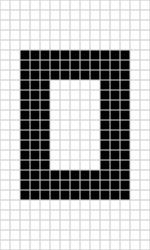
\includegraphics[height=1in]{./figures/hands-on6/zero.jpg}%
}
\subcaptionbox{The three vector types in the `zero' matrix.}[0.4\linewidth]{%
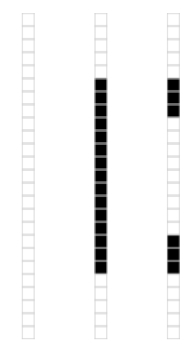
\includegraphics[height=1in]{./figures/hands-on6/zero-vecs.jpg}%
}
\end{center}
\end{figure}

If SVD is working like expected it should capture that feature of our input matrix, and we should be able to represent the entire image using just three singular values and their associated left- and right-singular vectors.

\begin{R}
> zsvd <- svd(z)
> round(zsvd$d,2)
 [1] 14.72  5.22  3.31  0.00  0.00  0.00  0.00  0.00  0.00  0.00  0.00  0.00  0.00  0.00
[15]  0.00
> D <- diag(zsvd$d[1:3])
> D
         [,1]     [,2]     [,3]
[1,] 14.72425 0.000000 0.000000
[2,]  0.00000 5.216623 0.000000
[3,]  0.00000 0.000000 3.314094
> U <- zsvd$u[,1:3]
> V <- zsvd$v[,1:3]
> newZ <- U %*% D %*% t(V)
> all.equal(newZ, z, check.attributes=F)
[1] TRUE

# and let's double check using the image() function
> image(1:15,1:25,t(newZ),col=c('black','white'),asp=1)
\end{R}

Our original matrix required $25 \times 15$ ($= 375$) storage elements. Using the SVD we can represent the same data using only $15 \times 3 + 25 \times 3 + 3 = 123$ units of storage (corresponding to the truncated U, V, and D in the example above). Thus our SVD allows us to represent the same data with at less than $1/3$ the size of the original matrix. In this case, because all the singular values after the 3rd were zero this is a lossless data compression procedure.


\subsection{Noise filtering using SVD}

The file |noisy-zero.dat| is the same 'zero' image, but now sprinkled with Gaussian noise draw from a normal distribution ($N(0,0.1)$. As in the data compression case we can use SVD to approximate the input matrix with a lower-dimensional approximation. Here the SVD is `lossy' as our approximation throws away information.  In this case we hope to choose the approximating dimension such that the information we lose corresponds to the noise which is `polluting' our data.

\begin{R}
> nz <- as.matrix(read.delim('noisy-zero.dat',header=F))
> dim(nz)
[1] 25 15
> x <- 1:15
> y <- 1:25
# create a gray-scale representation of the matrix
> image(x,y,t(nz),asp=1,xlim=c(1,15),ylim=c(1,25),col=gray(seq(0,1,0.05)))
> round(nz.svd$d,2)
 [1] 13.63  4.87  3.07  0.40  0.36  0.31  0.27  0.26  0.21  0.19  0.13  0.11  0.09  0.06
[15]  0.04
# as before the first three singular values dominate
> nD <- diag(nz.svd$d[1:3])
> nU <- nz.svd$u[,1:3]
> nV <- nz.svd$v[,1:3]
> approx.nz <- nU %*% nD %*% t(nV)

# now plot the original and approximating matrix side-by-side
> par(mfrow=c(1,2))
> image(x,y,t(nz),asp=1,xlim=c(1,15),ylim=c(1,25),col=gray(seq(0,1,0.05)))
> image(x,y,t(approx.nz),asp=1,xlim=c(1,15),ylim=c(1,25),col=gray(seq(0,1,0.05)))
\end{R}

As you can see from the images you created the approximation based on the approximation based on the SVD manages to capture the major features of the matrix and filters out much of (but not all) the noise.

\section{Image Approximation Using SVD in R}

R doesn't have native support for common image files like JPEG and PNG.  However, there are a couple of packages we call install that will allow us to read in such files and treat them as matrices:
%
\begin{R}
> install.packages("png", dependencies=T)
> install.packages("jpeg", dependencies=T)
\end{R}

The |png| and |jpeg| libraries provide simple functions for reading and writing image files.  The following code shows how to read in the |chesterbw.jpg| image which can be found in the course datasets. %The |ReadImages| provides more functions for manipulating image data, including functions for converting color images to grayscale, and for normalizing image values so they conform to what R expects for raster images.


The function |grid.raster| in the |grid| library can be used to draw the matrix of image data returned from the |readJPEG|.  There is also a lower-level |rasterImage()| function that can be used to draw images, as shown below. The |image()| function included in R base will also draw images, but to do so conveniently we'll write a simple wrapper function called |GreyscaleImage()|.

%
\begin{R}
> library(jpeg)
> img <- readJPEG("chesterbw.jpg")
> dim(img)
[1] 556 605
> typeof(img)
[1] "double"
> class(img)
[1] "matrix"
> ny <- dim(img)[1]  # rasterImage will draw rows along vertical axis
> nx <- dim(img)[2]
> max.pixels <- max(nx,ny)
> plot(0:max.pixels, 0:max.pixels, type='n', xlab='', ylab='',asp=1)
> ?rasterImage
> rasterImage(img, 0, 0, nx, ny)
> library(grid) # provides grid.raster function
> ?grid.raster
> grid.raster(img)  # more convenient but less flexible than rasterImage
> GreyscaleImage <- function(im){
+    rotated <- t(im[rev(1:nrow(im)), 1:ncol(im)])
+    image( rotated, col= grey(seq(0,1, length=256)), useRaster=TRUE )
+ }
> GreyscaleImage(img)
\end{R}
The output of the code above is shown in Fig~\ref{fig:chester}.
\begin{figure}[ht!]
  \center{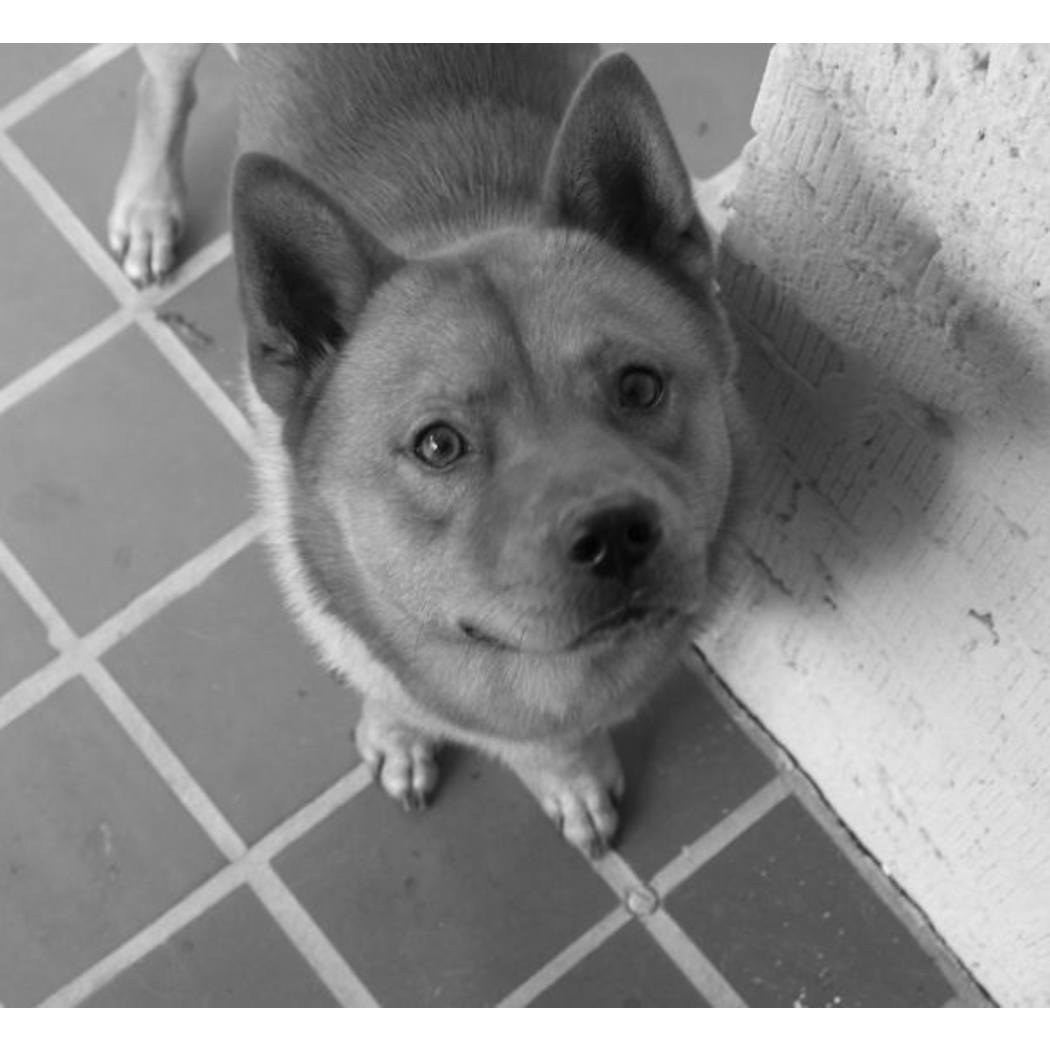
\includegraphics[width=0.28\textwidth]{./figures/hands-on6/fig-chesterorig.pdf}}
  \caption{My ever-faithful companion Chester.\label{fig:chester}}
\end{figure}


Now we'll use SVD to create a low-dimensional approximation of this image.
%
\begin{R}
> img.svd <- svd(img)
> U <- img.svd$u
> S <- diag(img.svd$d)
> Vt <- t(img.svd$v)

> U15 <- U[,1:15]  # first 15 left singular vectors
> S15 <- S[1:15,1:15]  # first 15 singular values
> Vt15 <- Vt[1:15,]  # first 15 right singular values, NOTE: we're getting rows rather than columns here

> approx15 <- U15 %*% S15 %*% Vt15
> GreyScaleImage(approx15)
\end{R}
%
The output of our approximate image is shown in Fig~\ref{fig:chester15}.
\begin{figure}[ht!]
  \center{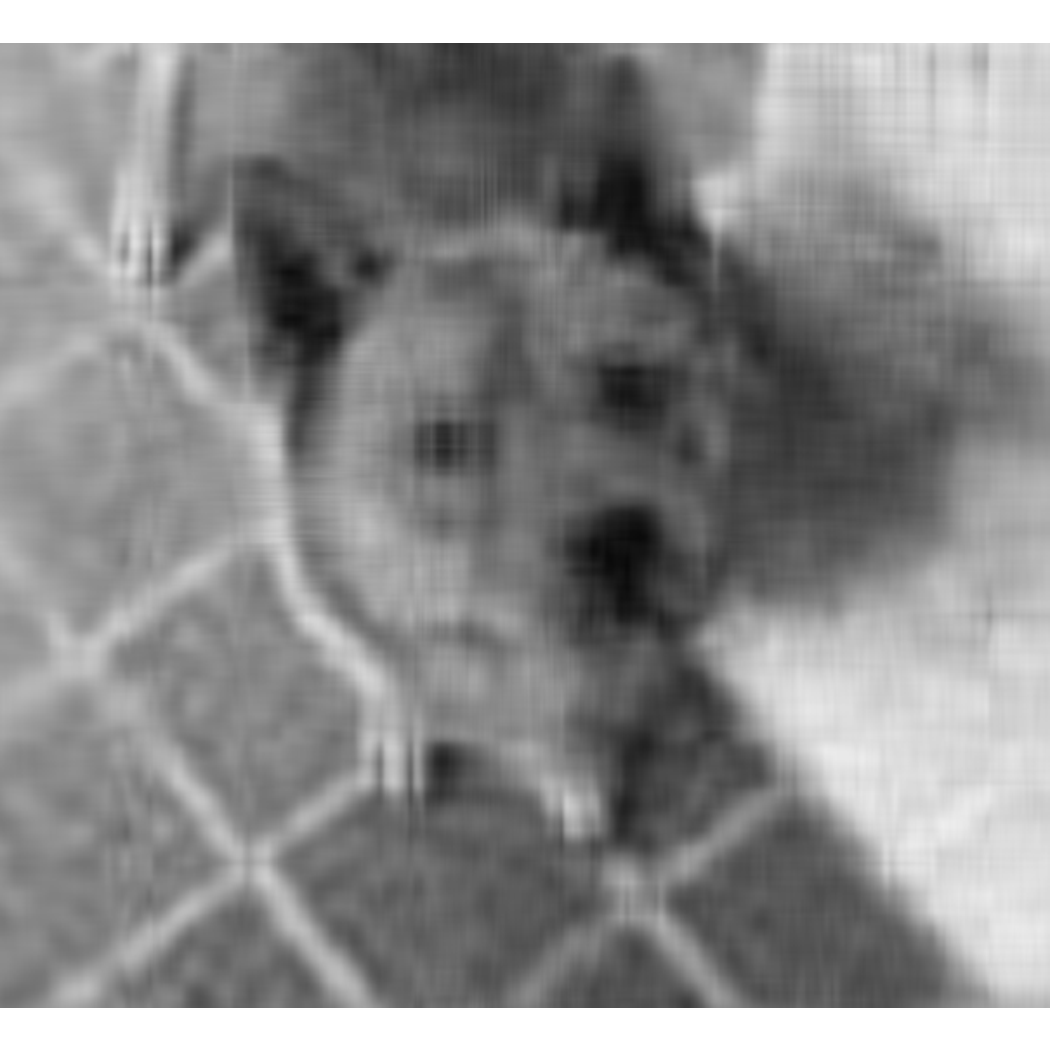
\includegraphics[width=0.28\textwidth]{./figures/hands-on6/fig-chesterapprox15.pdf}}
  \caption{A low-dimensional approximation of Chester.\label{fig:chester15}}
\end{figure}


Above we created a rank 15 approximation to the rank 556 original image matrix. This approximation is crude (as judged by the visual quality of the approximating image) but it does represent a very large savings in space. Our original image required the storage of $605 \times 556 = 336380$ integer values. Our approximation requires the storage of only $15 \times 556 + 15 \times 605 + 15 = 17430$ integers. This is a saving of roughly 95\%. Of course, as with any lossy compression algorithm, you need to decide what is the appropriate tradeoff between compression and data loss for your given application.

Finally, let's look at the `error term' associated with our approximation, i.e. what we \emph{did not} capture in the 15 singular vectors.
%
\begin{R}
> img.diff <- img - approx15
> GreyScaleImage(img.diff)
\end{R}
%
An image representing the information our approximation didn't capture is shown in Fig~\ref{fig:chesterdiff}.
%
\begin{figure}[ht!]
  \center{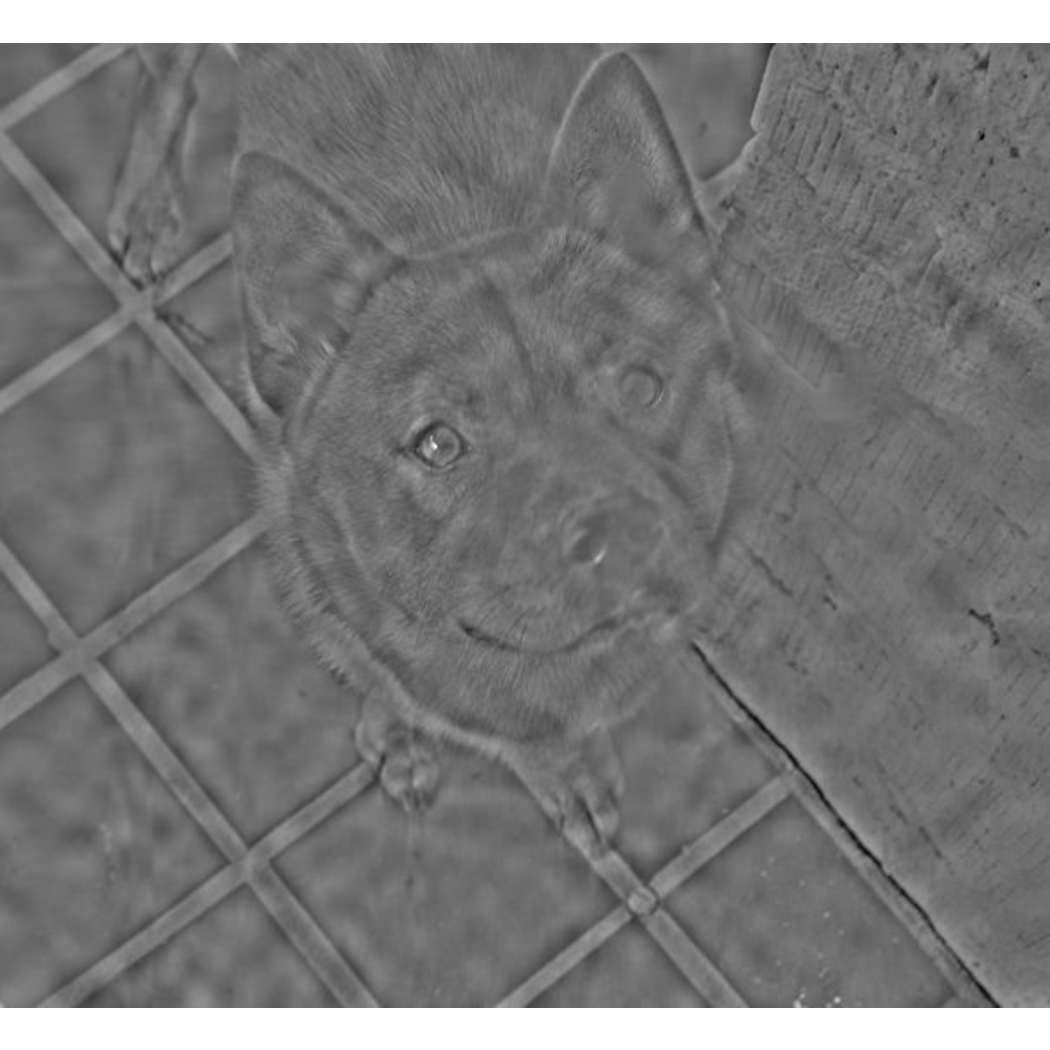
\includegraphics[width=0.28\textwidth]{./figures/hands-on6/fig-chesterdiff15.pdf}}
  \caption{A representation of the information \emph{not} captured by our approximation.\label{fig:chesterdiff}}
\end{figure}
  

\begin{assignment}
\small
Write a function, |svd_img()|, that automates the creation of a lower dimensional approximation of a grayscale image using SVD.
%
\begin{enumerate}
  \item Your function should take as input a matrix representing the original image and an integer specifying the approximating dimension -- i.e. function will be called as \verb|svd_img(imgmtx,dim)|.

  \item Your function should return a list of two objects: 1) an array representing the approximated image; and 2) an array representing the difference between the original and approximating images (i.e. original - approximation).

  \item Test your function on various images using a variety of approximating dimensions (e.g. 5,10, 25, 50, 100, 250) on the \verb|chesterbw.jpg| image.
\end{enumerate}


In addition to your code consider the following questions:
%
\begin{itemize}
\item When analyzing \texttt{chesterbw.jpg}, at some approximating dimensions you'll notice interesting artifacts. How do these relate to the original image?

\item What is the lowest approximating dimension where you would you consider the image to be recognizable as a dog?

\item At what approximating dimension would you judge the  image to be ``close enough"  to the original by the casual observer? What is the storage saving of this approximation relative to the original image?

\item How does the difference array change as the approximating dimension changes? Is there a particular type of image information that seems most prominent in the difference array?
\end{itemize}


\end{assignment}






% \chapter{ANOVA and Discriminant Analysis}
% 
\section{ANOVA in R}

We'll start our introduction to ANOVA in R by reconstructing the example used in the lectures slides:

\begin{R}
> y <- c(20, 17, 17, 21, 16, 14, 17, 16, 15, 8, 11, 8)
> groups <- c(1,1,1, 2,2,2, 3,3,3, 4,4,4)
> group.factor <- as.factor(groups)
\end{R}
%
Since we're doing this example by hand, let's check that our entries were correct by comparing the grand and group means to the example in the slides:
%
\begin{R}
> mean(y)  # grand mean
[1] 15

# means of each group
> mean(y[group.factor == 1])
[1] 18
> mean(y[group.factor == 2])
[1] 17
> mean(y[group.factor == 3])
[1] 16
> mean(y[group.factor == 4])
[1] 9
\end{R}

The |aov()| function in R is suitable for doing ANOVA with balanced designs.
\begin{R}
> ex.anova <- aov(y ~ group.factor)
> ex.anova
Call:
   aov(formula = y ~ group.factor)

Terms:
                group.factor Residuals
Sum of Squares           150        40
Deg. of Freedom            3         8

Residual standard error: 2.236068 
Estimated effects may be unbalanced
> summary(ex.anova)
             Df Sum Sq Mean Sq F value  Pr(>F)   
group.factor  3    150      50      10 0.00441 **
Residuals     8     40       5                   
---
Signif. codes:  0 ‘***’ 0.001 ‘**’ 0.01 ‘*’ 0.05 ‘.’ 0.1 ‘ ’ 1   
> coefficients(ex.anova)
  (Intercept) group.factor2 group.factor3 group.factor4 
           18            -1            -2            -9 
\end{R}

The ANOVA table shown by |summary()| looks the same as what I presented in the slides, but the model coefficients don't look the same because by default |aov()| uses dummy coding. To see how R creates contrasts from our grouping variable use the |contrasts()| function:
\begin{R}
> contrasts(group.factor)
  2 3 4
1 0 0 0
2 1 0 0
3 0 1 0
4 0 0 1
\end{R}
%
We can interpret the above as saying that samples from group 1 get coded as `0 0 0', those from group 2 as `1 0 0', etc.

We can  use |contrasts()| in combination with |contr.sum()| to change this to effect coding. The argument to |contr.sum()| should be the total number of groups:
%
\begin{R}
> contrasts(group.factor) <- contr.sum(4)
> contrasts(group.factor)
  [,1] [,2] [,3]
1    1    0    0
2    0    1    0
3    0    0    1
4   -1   -1   -1
\end{R}
%
Now that we've changed the matrix of contrasts, let's refit the model:
\begin{R}
> anova.2 <- aov(y ~ group.factor)
> summary(anova.2)
             Df Sum Sq Mean Sq F value  Pr(>F)   
group.factor  3    150      50      10 0.00441 **
Residuals     8     40       5                   
---
Signif. codes:  0 ‘***’ 0.001 ‘**’ 0.01 ‘*’ 0.05 ‘.’ 0.1 ‘ ’ 1 
> coefficients(anova.2)
  (Intercept) group.factor1 group.factor2 group.factor3 
           15             3             2             1 
\end{R}

\subsection{ANOVA via Multiple Regression}

In lecture we discussed how ANOVA can be fit as a multiple regression, using grouping variables as the predictor variables.  Let's confirm that, first by hand and then using the |lm()| function:
\begin{R}
> Y <- matrix(y)
> X <- model.matrix(~group.factor)  # note the leading tilde
>    # X will be effect coding if you used the contr.sum function above
>    # otherwise will be dummy coding
> X
   (Intercept) group.factor1 group.factor2 group.factor3
1            1             1             0             0
2            1             1             0             0
3            1             1             0             0
4            1             0             1             0
5            1             0             1             0
6            1             0             1             0
7            1             0             0             1
8            1             0             0             1
9            1             0             0             1
10           1            -1            -1            -1
11           1            -1            -1            -1
12           1            -1            -1            -1
attr(,"assign")
[1] 0 1 1 1
attr(,"contrasts")
attr(,"contrasts")$group.factor
  [,1] [,2] [,3]
1    1    0    0
2    0    1    0
3    0    0    1
4   -1   -1   -1

> 
> b <- solve(t(X) %*% X) %*% t(X) %*% Y
> b
              [,1]
(Intercept)     15
group.factor1    3
group.factor2    2
group.factor3    1
> 
> yhat <- X %*% b
> yhat.ctr <- yhat - mean(yhat)
> len.yhat <- t(yhat.ctr) %*% yhat.ctr
> dim.yhat <- 3
> 
> e <- Y - yhat
> len.e <- t(e) %*% e
> dim.e <- 8
> 
> F.stat <- (dim.e * len.yhat)/(dim.yhat * len.e)
> F.stat
     [,1]
[1,]   10
> ?FDist  # read the docs on the F distribution functions

# probability of observing the F, with given degrees of freedom
> pf(F.stat, 3, 8, lower.tail = FALSE)
[1] 0.004407445
\end{R}

And now, more compactly with the |lm()| function:
\begin{R}
> a.lm <- lm(y ~ group.factor)
> anova(a.lm)
Analysis of Variance Table

Response: y
             Df Sum Sq Mean Sq F value   Pr(>F)   
group.factor  3    150      50      10 0.004407 **
Residuals     8     40       5                    
---
Signif. codes:  0 ‘***’ 0.001 ‘**’ 0.01 ‘*’ 0.05 ‘.’ 0.1 ‘ ’ 1 
> summary(a.lm)

Call:
lm(formula = y ~ group.factor)

Residuals:
   Min     1Q Median     3Q    Max 
 -3.00  -1.00  -1.00   1.25   4.00 

Coefficients:
              Estimate Std. Error t value Pr(>|t|)    
(Intercept)    15.0000     0.6455  23.238 1.25e-08 ***
group.factor1   3.0000     1.1180   2.683   0.0278 *  
group.factor2   2.0000     1.1180   1.789   0.1114    
group.factor3   1.0000     1.1180   0.894   0.3972    
---
Signif. codes:  0 ‘***’ 0.001 ‘**’ 0.01 ‘*’ 0.05 ‘.’ 0.1 ‘ ’ 1 

Residual standard error: 2.236 on 8 degrees of freedom
Multiple R-squared: 0.7895, Adjusted R-squared: 0.7105 
F-statistic:    10 on 3 and 8 DF,  p-value: 0.004407 
\end{R}

\subsection{Graphical Depictions of ANOVA}

The |granova| package provides nice graphical representations of ANOVA. We'll apply this to a dataset called |genotypes| available in the |MASS| package (part of the basic R installation).  As described in the R help, rats with four different genotypes (A, B, I, and J) were separated from their natural mothers at birth, and give to foster mothers to rear.  There are two grouping variables we can explore here, the genotype of the foster mother and that of the litter.
\begin{R}
> install.packages("granova", dependencies=T)
> library(MASS)
> attach(genotype) # read about attach/detach in the docs
> aov.litter <- aov(Wt ~ Litter)
> summary(aov.litter)
            Df Sum Sq Mean Sq F value Pr(>F)
Litter       3     60   20.05   0.283  0.838
Residuals   57   4040   70.88               
> g.litter <- granova.1w(Wt, Litter)


> aov.mother <- aov(Wt ~ Mother)
> summary(aov.mother)
            Df Sum Sq Mean Sq F value  Pr(>F)   
Mother       3    772   257.2   4.405 0.00743 **
Residuals   57   3329    58.4                   
---
Signif. codes:  0 ‘***’ 0.001 ‘**’ 0.01 ‘*’ 0.05 ‘.’ 0.1 ‘ ’ 1 
> g.mother <- granova.1w(Wt, Mother)
\end{R}
%
% \begin{R}
% > install.packages("granova", dependencies=T)
% > attach(iris)  # read about attach/detach in the docs
% > aov.sl <- aov(Sepal.Length ~ Species)
% > summary(aov.sl)
%              Df Sum Sq Mean Sq F value Pr(>F)    
% Species       2  63.21  31.606   119.3 <2e-16 ***
% Residuals   147  38.96   0.265                   
% ---
% Signif. codes:  0 ‘***’ 0.001 ‘**’ 0.01 ‘*’ 0.05 ‘.’ 0.1 ‘ ’ 1 
% > granova.1w(Sepal.Length, Species)
% $grandsum
%     Grandmean        df.bet       df.with        MS.bet       MS.with        F.stat 
%          5.84          2.00        147.00         31.61          0.27        119.26 
%        F.prob SS.bet/SS.tot 
%          0.00          0.62 

% $stats
%            Size Contrast Coef Wt'd Mean Mean Trim'd Mean Var. St. Dev.
% setosa       50         -0.84      5.01 5.01        5.00 0.12     0.35
% versicolor   50          0.09      5.94 5.94        5.91 0.27     0.52
% virginica    50          0.74      6.59 6.59        6.55 0.40     0.64
% \end{R}

The output of the |granova.1w()| function is shown below. Use your common sense and the |granova.1w| docs to understand what the different elements of the plot mean.  For more details about the |granova| plots check out the paper the authors have made \href{http://rmpruzek.com/wp-content/uploads/2011/07/ElementalGraphicsForANOVA.finalJune11.pdf}{available on the web}.

\begin{figure}[ht!]
  \center{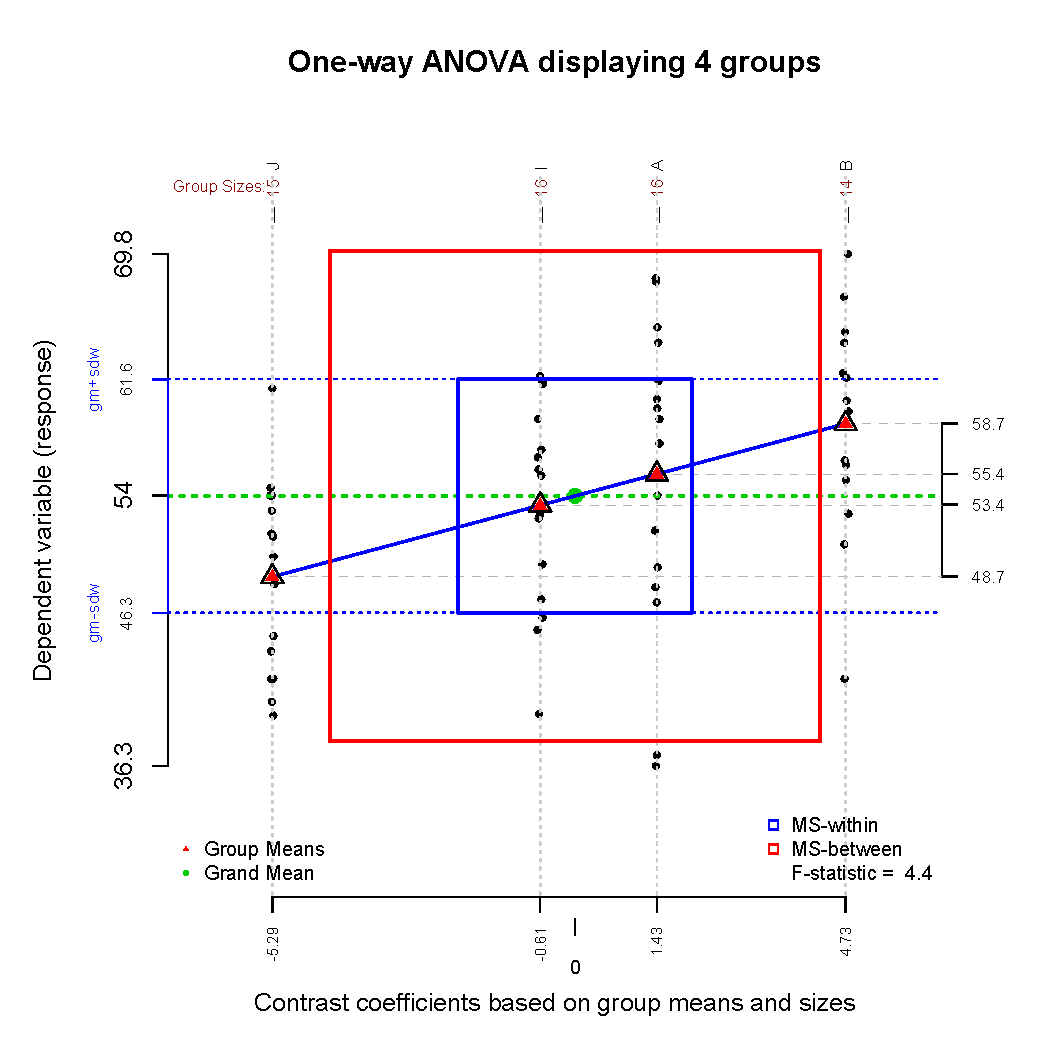
\includegraphics[width=0.5\textwidth]{./figures/hands-on7/fig-granova.pdf}}
  \caption{A graphical representation of a one-way ANOVA, created using the \texttt{granova} package.\label{fig:granova}}
\end{figure}


\section{Discriminant Analysis in R}

The function \texttt{lda()}, found in the R library \texttt{MASS}, carries out linear discriminant analysis (i.e. canonical variates analysis). 


\begin{R}
> library(MASS) #load the MASS package
> z <-lda(Species ~ Sepal.Length + Sepal.Width + Petal.Length + Petal.Width,
+           iris, prior=c(1,1,1)/3)
> z
Call:
lda(Species ~ Sepal.Length + Sepal.Width + Petal.Length + Petal.Width, 
    data = iris, prior = c(1, 1, 1)/3)

Prior probabilities of groups:
    setosa versicolor  virginica 
 0.3333333  0.3333333  0.3333333 

Group means:
           Sepal.Length Sepal.Width Petal.Length Petal.Width
setosa            5.006       3.428        1.462       0.246
versicolor        5.936       2.770        4.260       1.326
virginica         6.588       2.974        5.552       2.026

Coefficients of linear discriminants:
                    LD1         LD2
Sepal.Length  0.8293776  0.02410215
Sepal.Width   1.5344731  2.16452123
Petal.Length -2.2012117 -0.93192121
Petal.Width  -2.8104603  2.83918785

Proportion of trace:
   LD1    LD2 
0.9912 0.0088 
\end{R}

The |prior| argument given in the |lda()| function call isn't strictly necessary because by default the |lda| function will assign equal probabilities among the groups. However I included this argument call to illustrate how to change the prior if you wanted. The output give some simple summary statistics for the group means for each of the variables and then gives the coefficients of the canonical variates.  The `Proportion of trace' output above tells us that 99.12\% of the between-group variance is captured along the first discriminant axis.

\subsection{Shorthand Formulae in R}

You've encountered the use of model formulae in R several times, such as in the call to |lda()| above and when carrying out various regressions.  The document ``An Introduction to R" (distributed with R and available at the R project website) gives a concise summary and a number of examples of how to construct formulae in R (see \href{http://cran.r-project.org/doc/manuals/R-intro.html#Formulae-for-statistical-models}{Defining statistical models: formulae}).

Relevant to our current example is a shorthand way for specifying multiple variables in a formula. In the example above we called the |lda()| function with a formula of the form: 
\begin{R}
Species ~ Sepal.Length + Sepal.Width + ....
\end{R}

Writing the names of all those variables is tedious and error prone and would be unmanageable if we were analyzing a data set with tens or hundreds of variables. Luckily we can use the shorthand name `|.|' to specify all other variables in the data frame except the variable on the left.  For example, we can rewrite the |lda()| call above as:

\begin{R}
> z <- lda(Species ~ ., data = iris, prior = c(1,1,1)/3)
\end{R}

\subsection{Fine Tuning Your Plot}

To get a graphical representation of the specimens in the space of the canonical variates you can use the |plot()| function on the object returned by the call to |lda()|.

\begin{R}
> plot(z) # 2D scatter plot of specimens in CVs 1 and 2
> plot(z, abbrev=T) # use abbreviated group names
\end{R}

You can also create a plot to look at group variation along just the first canonical variate:

\begin{R}
> plot(z, dimen=1,type='both') # plot histograms and density plots for each group along 1st CV 
\end{R}


The plot call on the object returned by |lda()| allows some additional customization of the plot, but the extent of graphical tuning is limited:

\begin{R}
> plot(z, abbrev=T, xlab='CV1', ylab='CV2') # change the x- and y- labels
\end{R}

If you want to do any more fine tuning of the plot you'll have to calculate the CV scores from the coefficients and reconstruct the plot to your liking. Below I give an example of how to do that:

\begin{R}
> iris.data <- subset(iris,select=-Species)
> iris.mtx <- as.matrix(iris.data)
> dim(iris.mtx)
[1] 150   4
> iris.cv <- iris.mtx %*% z$scaling # gives scores in the CV space
> dim(iris.cv)
[1] 150   2
> group.symbols <- (1:3)[iris$Species] # specify the symbols for each group
> plot(iris.cv, pch=group.symbols, asp=1, xlab="CV1", ylab="CV2")
\end{R}

The definition of |group.symbols| and the use of the |pch| argument require a little explanation. |pch| is short-hand for `plotting  character' and specifies the symbols used to represent each observation in the plot.  These symbols can either be letters or integers in the range 0-25. The integers refer to a standard set of symbols shapes defined in R. Figure~1 gives those symbols.

\begin{figure}
\begin{center}

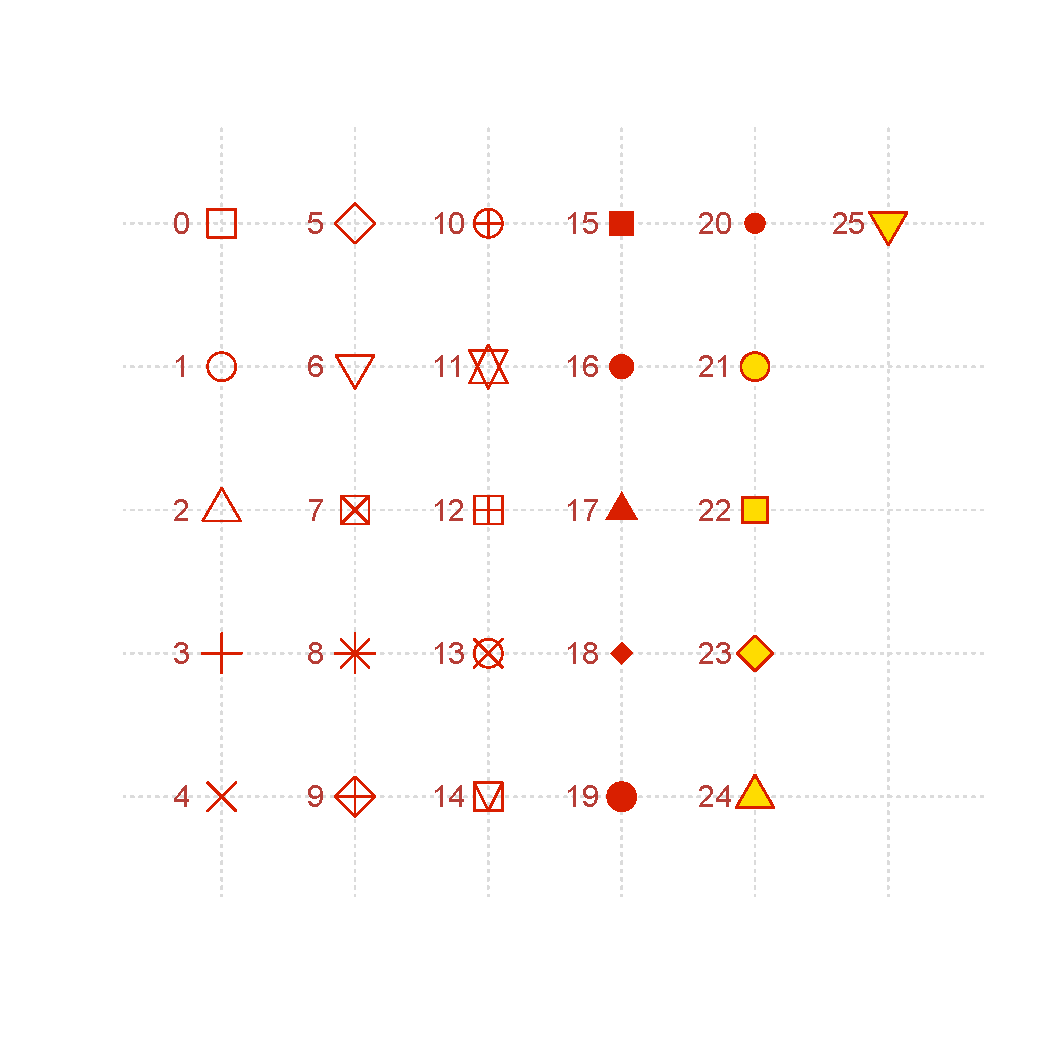
\includegraphics[width=0.5\columnwidth]{./figures/hands-on7/pch-symbols}

\end{center}
\caption{Standard R symbols, and their corresponding integer values, accessible via the \texttt{pch} argument to plot.}
\end{figure}

If you'd like to see a function that prints out all the standard symbols type |?points| and check out the |pchShow| function defined in the example at the bottom of the documentation page.  To see this example in action type |example(points)|. After typing |example(points)| you can call the |pchShow| function directly (that's how I generated the figure).

The |group.symbols <- ...| line constructs a vector of length $n$ (where $n$ is the length of the \lstinline|iris$Species| vector) where each element of the |group.symbols| vector has the value 1, 2 or 3 according to which species the corresponding specimen represents.  A simpler example might make this clearer:

\begin{R}
> sexes = as.factor(c('M','F','F','M','F'))
> sexes
[1] M F F M F
Levels: F M
> c("a","b")[sexes]
[1] "b" "a" "a" "b" "a"
\end{R}

Here I created a simple example involving five specimens where each specimens was categorized by sex. The |as.factor| function tells R to treat the characters in the vector as factor levels. I then assigned each specimen a label, either``a" or ``b" depending on its sex.  If I wanted to extend that example to our three species iris data set I could do something like:

\begin{R}
> group.symbols = c("a","b","c")[iris$Species]
> plot(iris.cv, pch=group.symbols, cex=0.75, asp=1, xlab="CV1", ylab="CV2")
\end{R}

This draws each specimen with the label ``a", ``b", or ``c" depending on which species it is assigned to. Notice that in the last example I used the |cex| argument to make the symbols smaller than normal.  

What if i wanted to also plot the group means in the canonical variate space?  The following example shows how to do that:

\begin{R}
> group.symbols = c(0,2,4)[iris$Species] # I switched back to symbols 
> group.colors = c('red','darkorange','blue')[iris$Species] # I also want to use colors 
> cv1.means <- tapply(iris.cv[,1], iris$Species, mean)
> cv1.means
    setosa versicolor  virginica 
  5.502493  -3.930156  -7.887657 
> cv2.means <- tapply(iris.cv[,2], iris$Species, mean)
> cv2.means
    setosa versicolor  virginica 
  6.876606   5.933573   7.174239 
> plot(iris.cv, pch=group.symbols, cex=0.75, asp=1, 
+       xlab="CV1", ylab="CV2", col=group.colors)
> points(cv1.means, cv2.means, pch=16, cex=1.5, col='black')
\end{R}

Note the use of the |points()| function. This function draws on top of rather than erasing the previous plot.  Note too the use of the |col| argument in the |plot()| call to specify different colors.  If you'd like to see a chart of all the colors in R check out this web page: \href{http://research.stowers-institute.org/efg/R/Color/Chart/}{A Chart of R Colors}.

I stated in lecture that for the canonical variate diagram we can estimate the $100(1-\alpha)$ confidence region for a group mean as a circle centered at the mean having a radius $(\chi^{2}_{\alpha,r}/n_i)^{1/2}$ where $r$ is the number of canonical variate dimensions considered. Using similar reasoning the $100(1-\alpha)$ confidence region for the whole population is given by a hypersphere centered at the mean with radius $(\chi^{2}_{\alpha,r})^{1/2}$.  
To calculate these confidence regions you could look up the appropriate value of the the  $\chi^2$ distribution in a book of statistical tables, or we can use the |qchisq()| function which gives the inverse cumulative probability distribution for the $\chi^2$ function:

\begin{R}
> chi2 = qchisq(0.05,2, lower.tail=F)
> chi2
[1] 5.991465
> group.lengths = tapply(iris$Species, iris$Species, length)
> group.lengths
    setosa versicolor  virginica 
        50         50         50 
> mean.radii = sqrt(chi2/group.lengths)
> pop.radii = rep(sqrt(chi2),3)
> help.search("circle")  # I don't remember off hand how to draw circles so let's look it up
> library(tripack) # Let's use the circles function in the 'tripack' package
> circles(cv1.means, cv2.means, pop.radii,lty='dashed') 
> circles(cv1.means, cv2.means, mean.radii,lty='dotted')
\end{R}

Let's put the finishing touch on our plots by adding some color coded rug plots to the first CV axis. For completeness I'll include all the previous steps used to generate the plot:

\begin{R}
> plot(iris.cv, pch=group.symbols, cex = 0.75, asp=1, xlab="CV1", ylab="CV2", col=group.colors)
> points(cv1.means, cv2.means, pch=16, cex=1.5,col='red')
> circles(cv1.means, cv2.means, pop.radii,lty='dashed')
> circles(cv1.means, cv2.means, mean.radii, lty='dotted')
> rug(iris.cv[,1][iris$Species=="setosa"],col="red")
> rug(iris.cv[,1][iris$Species=="versicolor"],col="darkorange")
> rug(iris.cv[,1][iris$Species=="virginica"],col="blue")
> title("Canonical Variates Analysis\nof Anderson's Iris Data")
\end{R}


If you did everything right (and I cut and pasted correctly!) you should get a plot that looks like \cref{fig:cva}.  If I was going to be repeatedly generate these types of plots I would wrap up the key steps discussed above into a convenient function.


\begin{figure}
\begin{center}
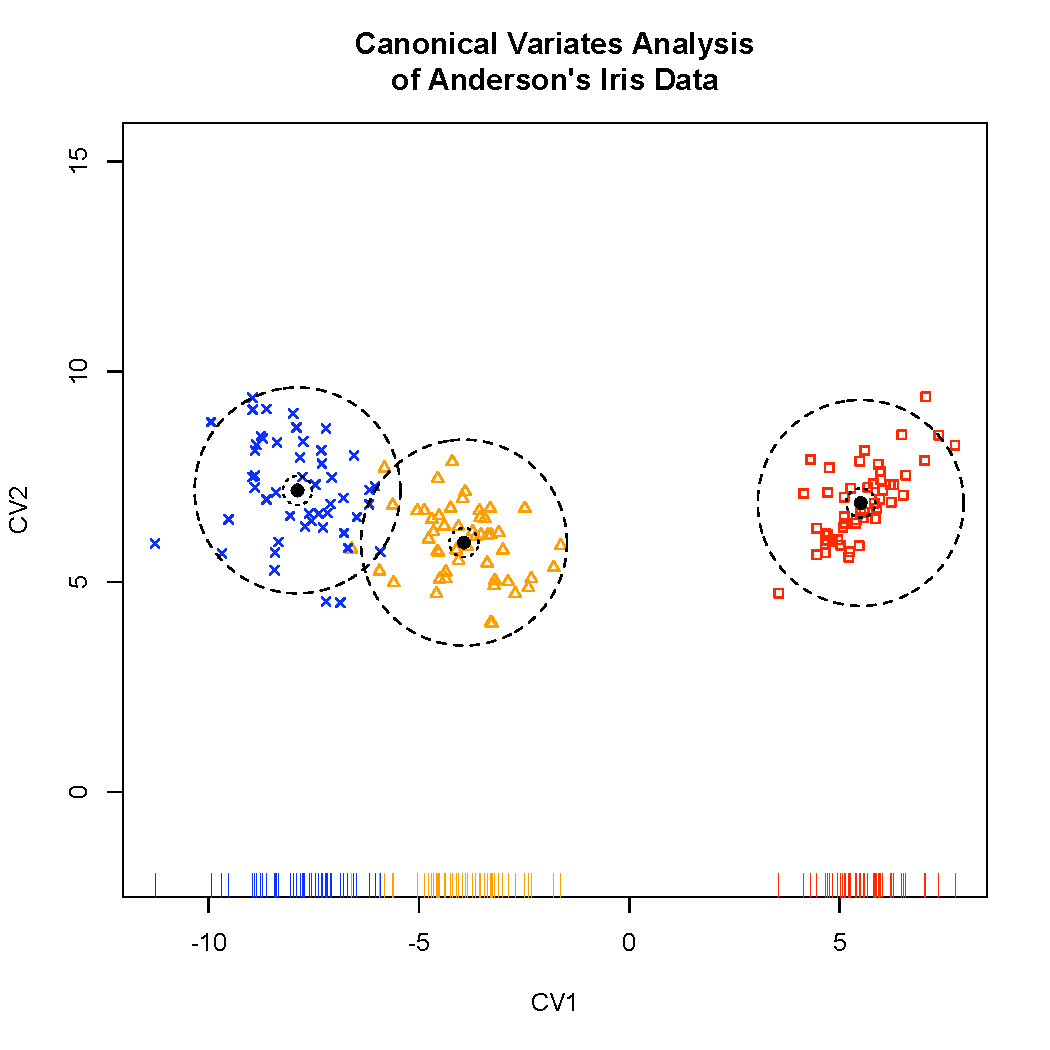
\includegraphics[height=0.5\columnwidth]{./figures/hands-on7/iris-cva-fancy}
\end{center}
\caption{Ordination of iris specimens in the space of the first two canonical variates.  The dashed circles surrounding each species distribution give the approximate 95\% tolerance regions for the population distributions. See text for details on the construction of this plot.} \label{fig:cva}.
\end{figure} 

\subsection{Calculating the Within and Between Group Covariance Matrices}

The |lda()| function conveniently carries out the key steps of a canonical variates analysis for you.  However, what if we wanted some of the intermediate matrices relevant to the analysis such as the within- and between group covariances matrices? The code below shows you how to calculate these:

\begin{R}
> g = iris$Species
> group.means <- rowsum(iris.mtx, g)/as.vector(table(g))
> group.means
           Sepal.Length Sepal.Width Petal.Length Petal.Width
setosa            5.006       3.428        1.462       0.246
versicolor        5.936       2.770        4.260       1.326
virginica         6.588       2.974        5.552       2.026
> Dwin <- iris.mtx - group.means[g,]
> nobs <- dim(iris.mtx)[1]
> ngroups <- length(levels(g))
> win.cov <- 1/(nobs-ngroups) * t(Dwin) %*% Dwin
> btw.cov.unweighted <- cov(group.means)
\end{R}

Having now calculated the within group covariance matrix we can calculate the Mahalanobis distance between the means of each group as follows:

\begin{R}
> mahalanobis(group.means, group.means[1,], win.cov)
    setosa versicolor  virginica 
   0.00000   89.86419  179.38471 
> mahalanobis(group.means, group.means[2,], win.cov)
    setosa versicolor  virginica 
  89.86419    0.00000   17.20107 
> mahalanobis(group.means, group.means[3,], win.cov)
    setosa versicolor  virginica 
 179.38471   17.20107    0.00000 
\end{R}

\medskip
\begin{assignment}
\small

Identify a paper from the literature relevant to your research interests that employs one or more of the following multivariate statistical techniques:

\begin{enumerate}
\item Multivariate regression
\item Principal Component Analysis
\item Singular Value Decomposition
\item Canonical Variate Analysis (or an alternate discriminant function)
\end{enumerate}

Write a short report discussing the use of these techniques in the paper and how the application of these methods contributed to the author's conclusions or understanding of the data.  Your report should touch on any assumptions (explicit or implicit) that are relevant to the statistical analysis and discuss whether you feel the author's conclusions are justified or well supported (again based on the statistical anlaysis).  Did the author(s) provide sufficient detail for you repeat the analysis if you had the data?  Have the authors(s) made their multivariate data set available?

\medskip
Include in your report a brief outline (bullet points) that lays out the key steps (e.g. handling of missing data, normalization) and the primary R functions that you would use to repeat the analysis yourself. You don't actually have to carry out the analysis, but rather give a `road map' for doing so.


\end{assignment}




% \chapter{Introduction to Python}
% 

%!TEX root = ./hands-on1.tex

\section{Starting the Python interpretter}

The Python interpretter can be started in a number of ways. The simplest
way is to open a shell (terminal) and type |python|. Go ahead and do
this to make sure you have a working version of the default Python
interpretter available on your system. From within the default
interpretter you can type |Ctrl-d| (Unix, \OSX) or
|Ctrl-z| (Windows) to stop the interpretter and return to the
command line.

For interactive use, the default interpretter isn't very feature rich,
so the Python community has developed a number of GUIs or shell
interfaces that provide more functionality. For this class we will be
using an interface called \href{http://ipython.org/}{IPython}. Recent versions of IPython provides terminal and GUI-based shells as well as a web-browser interface called the IPython Notebook. 

% The EPD installer will place a number of shortcuts on your Start
% Menu or in Launchpad on OS X 10.7, including ones that read
% |PyLab| and |QtConsole|. These are a terminal based
% and GUI based versions of IPython respectively, both of which
% automatically load key numerical and plotting libraries. Click on both
% of these icons to compare their interfaces.

% To get the functionality of |PyLab| from the terminal, run the
% following command from your shell:
% %
% \begin{bash}
% ipython --pylab
% \end{bash}
% %
% To get the equivalent of |QtConsole| you can run ipython with
% the following arguments:
% %
% \begin{bash}
% ipython qtconsole --pylab
% \end{bash}
% %
% If you'd prefer a dark background, call QtConsole as so:
% %
% \begin{bash}
% ipython qtconsole --pylab --colors=linux
% \end{bash}
% %
% QtConsole is a recent addition to IPython and there may still be bugs to
% be sorted out, but it provides some very nice features like `tooltips'
% (shows you useful information about functions as you type) and the
% ability to embed figures and plots directly into the console, and the
% ability to save a console session as a web page (with figures
% embedded!).

% \subsection{Quick IPython tips}

% IPython has a wealth of features, many of which are detailed in its
% \href{http://ipython.org/documentation.html}{documentation}. There are
% also a number of videos available on the IPython page which demonstrate
% some of it's power. Here are a few key features to get you started and
% save you time:

% \begin{itemize}
% \item
%   \emph{Don't retype that long command!} --- You can scroll back and
%   forth through your previous inputs using the up and down arrow keys
%   (or |Ctrl-p| and |Ctrl-n|); once you find what you
%   were looking forward you can edit or change it. For even faster
%   searching, start to type the beginning of the input and then hit the
%   up arrow.
% \item
%   \emph{Navigate using standard Unix commands} --- IPython lets you use
%   standard Unix commands like |ls| and |cd| and
%   \lstinline!pwd! to navigate around your file system (even on Windows!)
% \item
%   \emph{Use \texttt{<Tab>} for command completion} ---
%   when your navigating paths or typing function names in you can hit the
%   |<Tab>| key and IPython will show you matching functions or
%   filenames (depending on context). For example, type
%   |cd ./<Tab>| and IPython will show you all the files and
%   subdirectories of your current working directory. Type a few of the
%   letters of the names of one of the subdirectories and hit
%   |<Tab>| again and IPython will complete the name if it finds
%   a unique match. Tab completeion allows you to very quickly navigate
%   around the file system or enter function names so get the hang of
%   using it.
% \end{itemize}


\section{Accessing the Documentation in Python}

Python comes with extensive HTML documentation and the Python
interpreter has a help function that works similar to R's
|help()|.
%
\begin{python}
>>> help(sum)
Help on built-in function sum in module __builtin__:

sum(...)
    sum(sequence, start=0) -> value

    Returns the sum of a sequence of numbers (NOT strings) plus the value
    of parameter 'start'.  When the sequence is empty, returns start.
\end{python}
%
IPython also lets you use proceed the function name with a question
mark:
%
\begin{python}
In [1]: ?sum
Type:       builtin_function_or_method
Base Class: <type 'builtin_function_or_method'>
String Form:<built-in function sum>
Namespace:  Python builtin
Docstring:
sum(sequence[, start]) -> value

Returns the sum of a sequence of numbers (NOT strings) plus the value
of parameter 'start' (which defaults to 0).  When the sequence is
empty, returns start.
\end{python}


\section{Using Python as a Calculator}

The simplest way to use Python is as a fancy calculator. Let's explore some simple arithmetic operations:
%
\begin{python}
>>> 2 + 10   # this is a comment
12
>>> 2 + 10.3
 12.300000000000001  # 0.3 can't be represented exactly in floating point precision
>>> 2 - 10
-8
>>> 1/2  # integer division
0
>>> 1/2.0  # floating point division
0.5
>>> 2 * 10.0
20.0
>>> 10**2  # raised to the power 2
100
>>> 10**0.5  # raised to a fractional power
3.1622776601683795
>>> (10+2)/(4-5)
-12
>>> (10+2)/4-5  # compare this answer to the one above 
-2
\end{python}
%
In addition to integers and reals (represented as floating points
numbers), Python knows about complex numbers:
%
\begin{python}
>>> 1+2j  # Engineers use 'j' to represent imaginary numbers
(1+2j)
>>> (1 + 2j) + (0 + 3j)
(1+5j)
\end{python}

Some things to remember about mathematical operations in Python:
\begin{itemize}
\item
  Integer and floating point division are not the same in Python.
  Generally you'll want to use floating point numbers.
\item
  The exponentiation operator in Python is |**|
\item
  Be aware that certain operators have precedence over others. For
  example multiplication and division have higher precedence than
  addition and subtraction. Use parentheses to disambiguate potentially
  confusing statements.
\item
  The standard math functions like |cos()| and
  |log()| are not available to the Python interpeter by
  default. To use these functions you'll need to |import| the
  math library as shown below.
\end{itemize}

For example:
%
\begin{python}
>>> 1/2
0
>>> 1/2.0
0.5    
>>> cos(0.5)
Traceback (most recent call last):
  File "<pyshell#2>", line 1, in -toplevel-
    cos(0.5)
NameError: name 'cos' is not defined
>>> import math  # make the math module available
>>> math.cos(0.5) # cos() function in the math module
0.87758256189037276
>>> pi   # pi isn't defined in the default namespace
Traceback (most recent call last):
  File "<pyshell#5>", line 1, in -toplevel-
    pi
NameError: name 'pi' is not defined
>>> math.pi # however pi is defined in math
3.1415926535897931
>>> from math import * # bring everything in the math module into the current namespace
>>> pi
3.1415926535897931
>>> cos(pi)
-1.0
\end{python}



\section{More Data Types in Python}

You've already seen the three basic numeric data types in Python -
integers, floating point numbers, and complex numbers. There are two
other basic data types - Booleans and strings.

Here's some examples of using the Boolean data type:
\begin{python}
>>> x = True
>>> type(x)
<type 'bool'>
>>> y = False
>>> x == y
False
>>> if x is True:
...     print 'Oh yeah!'
... 
Oh yeah!
>>> if y is True:
...     print 'You betcha!'
... else:
...     print 'Sorry, Charlie'
... 
Sorry, Charlie
>>>
\end{python}

\subsection{Comparison Operators Return Booleans}

The standard comparison operators for numerical values are available in Python. Comparison operators return Boolean values:
%
\begin{python}
>>> 4 < 5 # less than
True
>>> 4 > 3.99 # greater than
True
>>> 4 <= 4.0 # less than or equal to
True
>>> 4 >= 5 # greater than or equal to
False
>>> 4 == 4.0 # test equality
True
\end{python}


\subsection{Strings}
%
The string data type is used to represent ordered sets of characters, such as text:
%
\begin{python}
>>> s1 = 'It was the best of times'
>>> type(s1)
<type 'str'>
>>> s2 = 'it was the worst of times'
>>> s1 + s2  # string concatenation
'It was the best of timesit was the worst of times'
>>> s1 + ', ' + s2
'It was the best of times, it was the worst of times'
>>> 'times' in s1
True
>>> s3 = "You can nest 'single quotes' in double quotes"
>>> s4 = 'or "double quotes" in single quotes'
>>> s5 = "but you can't nest "double quotes" in double quotes"
  File "<stdin>", line 1
    s5 = "but you can't nest "double quotes" in double quotes"
                                   ^
SyntaxError: invalid syntax
\end{python}
%
Note that you can use either single or double quotes to specify strings.

\section{Simple data structures in Python: Lists}

Lists are the simplest `built-in' data structure in Python. List
represent ordered collections of arbitrary objects.
%
\begin{python}
>>> l = [2, 4, 6, 8, 'fred']
>>> l
[2, 4, 6, 8, 'fred']
>>> len(l)
5
\end{python}

Python lists are zero-indexed. This means you can access lists elements
|0| to |len(x)-1|.
%
\begin{python}
>>> l[0]
2
>>> l[3]
8
>>> l[5]
Traceback (most recent call last):
  File "<stdin>", line 1, in <module>
IndexError: list index out of range
\end{python}
%
You can use negative indexing to get elements from the end of the list:
\begin{python}
>>> l[-1] # the last element
'fred'
>>> l[-2] # the 2nd to last element
8
>>> l[-3] # ... etc ...
6
\end{python}

Python lists support the notion of `slices' - a continuous sublist of a
larger list. The following code illustrates this concept:
%
\begin{python}
>>> y = range(10)  # our first use of a function!
>>> y
[0, 1, 2, 3, 4, 5, 6, 7, 8, 9]
>>> y[2:8]
[2, 3, 4, 5, 6, 7]
>>> y[2:-1] # the slice
[2, 3, 4, 5, 6, 7, 8]
>>> y[-1:0] # how come this didn't work? 
[]
# slice from last to first, stepping backwards by 2
>>> y[-1:0:-2]  
[9, 7, 5, 3, 1]
\end{python}

\section{Using NumPy arrays}

The Python user community has developed a module called \numpy for efficient numerical computing in Python.  The basic data structure in the \numpy library is an array. Arrays can be used to reprsent both vectors and matrices, common mathematical structures we'll use throughout the course. Below are some examples illustrating the use of \numpy arrays:
\begin{python}
>>> from numpy import array # a third form of import 
>>> x = array([2,4,6,8,10])
>>> -x
array([ -2,  -4,  -6,  -8, -10])
>>> x ** 2
array([  4,  16,  36,  64, 100])
>>> pi * x # assumes pi is in the current namespace
array([  6.28318531,  12.56637061,  18.84955592,  25.13274123,  31.41592654])
>>> y = array([0, 1, 3, 5, 9])
>>> x + y
array([ 2,  5,  9, 13, 19])
>>> x * y
array([ 0,  4, 18, 40, 90])
>>> z = array([1, 4, 7, 11])
>>> x+z
Traceback (most recent call last):
  File "<stdin>", line 1, in <module>
ValueError: shape mismatch: objects cannot be broadcast to a single shape
\end{python}
%
The error above illustrates that basic arithmetic operations involving pairs of \numpy arrays in Python require that the arrays be of equal length.

Remember that lists and arrays in Python are zero-indexed rather than
one-indexed.
%
\begin{python}
>>> x
array([ 2,  4,  6,  8, 10])
>>> len(x)
5
>>> x[0]
2
>>> x[1]
4
>>> x[4]
10
>>> x[5]

Traceback (most recent call last):
  File "<pyshell#52>", line 1, in -toplevel-
    x[5]
IndexError: index out of bounds
\end{python}

\numpy arrays support the comparison operators and return arrays of
booleans.
\begin{python}
    >>> x < 5 
    array([ True, True, False, False, False], dtype=bool)
    >>> x >= 6 
    array([0, 0, 1, 1, 1])
\end{python}
%
\numpy also supports the combination of comparison and indexing
%
\begin{python}
>>> x[x < 5]  # get the elements of x where that are less than 5
array([2, 4])
>>> x[x >= 6]  # elements of x that are greater than or equal to 6
array([ 6,  8, 10])
>>> x[(x<4)+(x>6)]  # 'or'
array([ 2,  8, 10])
\end{python}
%
Note that Boolean addition is equivalent to `or' and Boolean
multiplication is equivalent to `and'.  There are also a variety of more complicated indexing functions
available for NumPy; see the
\href{http://docs.scipy.org/doc/numpy/reference/routines.indexing.html}{Indexing Routines} in the Numpy docs.

Most of the standard mathematical functions can be applied to NumPy
arrays however you must use the functions defined in the
\numpy module.
%
\begin{python}
>>> x
array([ 2,  4,  6,  8, 10])
>>> import math
>>> math.cos(x)

Traceback (most recent call last):
  File "<pyshell#67>", line 1, in -toplevel-
    math.cos(x)
TypeError: only length-1 arrays can be converted to Python scalars.
>>> import numpy
>>> numpy.cos(x)
array([-0.41614684, -0.65364362,  0.96017029, -0.14550003, -0.83907153])
\end{python}


% \section{Simple Plots in Python}

% The Matplotlib package is the de facto standard for producing
% publication quality scientific graphics in Python. Matplotlib is
% included with the Anaconda Python Distributions. Here are some simple plotting examples using matplotlib:
% %
% \begin{python}
% >>> from pylab import * # import all the functions from the pylab module of numpy
% >>> import numpy as np # use a shorter alias
% # load the turtle data using the numpy.loadtxt function 
% # skipping the first row (header) and the first column 
% >>> turt = np.loadtxt('turtles.txt', skiprows=1, 
%                       usecols=(1,2,3))
% >>> turt.shape
% (48, 3)
% # draw bivariate scatter plot
% >>> scatter(turt[:,0], turt[:,1])
% # give the axes some labels and a title for the plot
% >>> xlabel('Length')
% >>> ylabel('Width')
% >>> title('Turtle morphometry')
% \end{python}




% \chapter{Clustering Methods}
% 

\section{Hierarchical Clustering in R}

The function |hclust()| provides a simple mechanism for carrying out standard hierarchical clustering in R. The |method| argument determines the group distance function used (single linkage, complete linkage, average, etc.).

The input to |hclust()| is a dissimilarity matrix. The function |dist()| provides some of the basic dissimilarity measures (e.g. Euclidean, Manhattan, Canberra; see method argument of |dist()|) but you can convert an arbitrary square matrix to a distance object by applying the |as.dist()| function to the matrix.

\begin{R}
> iris.data <- subset(iris, select=-Species) 
> iris.cl <- hclust(dist(iris.data), method='single')
> plot(iris.cl) # plot a dendrogram
# let's improve the look a little bit
> plot(iris.cl, labels=iris$Species, cex=0.7)
> # use neg. values of hang to make labels on leaves line up
> plot(iris.cl, labels=iris$Species,  hang=-0.1, cex=0.7)
\end{R}

Other functions of interested related to dendrograms include |cuttree()| for cutting the tree at a specified height (or number of groups) and |identify()| for graphically highlighting a cluster of interest in a dendrogram.

\begin{R}
> plot(iris.cl, labels=iris$Species, cex=0.7)
                                           # identify fxn doesn't work in R-Studio
> interesting.cluster <- identify(iris.cl) # use left-mouse to choose, right-mouse to stop choosing
> interesting.cluster
# [output ommitted]
\end{R}

Fancy formatting of dendrogram plots in R is awkward. You need to use the |plot()| function in combination with the |as.dendrogram()| function to access many options. See the help for 'dendrogram' in R for a discussion of options and type |example(dendrogram)| to see some possibilities. A few of them are illustrated here:

\begin{R}
> plot(as.dendrogram(iris.cl)) # contrast this with plot(iris.cl)
> plot(as.dendrogram(iris.cl), horiz=T) # draw horizontally
> # here's one way to change the labels
> iris.cl$labels <- iris$Species
> levels(iris.cl$labels) <- factor(c("S","Ve","Vi"))
> iris.dend <- as.dendrogram(iris.cl)
> plot(iris.dend)
\end{R}

The |heatmap()| function combines a false color image of a matrix with a dendrogram. Here's we apply it to the yeast-subnetwork data set from previous weeks.

\begin{R}
> yeast <- read.delim('yeast-subnetwork-clean.txt')
> ymap <- heatmap(as.matrix(yeast), labRow=NA) # suppress the numerous row labels
> ymap <- heatmap(as.matrix(yeast),labRow=rownames(yeast)) # w/row labels, kinda messy

\end{R}

The R package |cluster| provides some slightly fancier clustering routines. The basic agglomerative clustering methods in |cluster| are accessed via the function |agnes()| 

Compare the results of different hierarchical clustering methods (single linkage, complete linkage, etc.) as applied to the iris data set using the hclust() or agnes() functions. For single and average linkage use both Euclidean and Manhattan distance as the dissimilarity measures.


\section{K-means Clustering in R}

The \texttt{kmeans()} function calculates standard k-means clusters in R.  The input is a data matrix (perhaps transformed before hand) and $k$, the number of clusters. Alternatively you can specify starting cluster centers. You can also run the algorithm multiple times with different random starting positions by using the \texttt{nstart} argument.

\begin{R}
# generate data set w/two groups (one of size 50, the other of size 75)
# note the different means and std dev between the two groups
> test.data <- rbind(matrix(rnorm(100, mean=0, sd=0.2),ncol=2), 
                  matrix(rnorm(150,mean=1,sd=0.5),ncol=2))
> colnames(test.data) <- c("x", "y")
> plot(test.data)
> cl <- kmeans(test.data, 2)
> names(cl)
[1] "cluster"  "centers"  "withinss" "size"    
> cl$cluster #  which cluster each object is assigned to
... output deleted ...
> plot(test.data, col = cl$cluster)
> cl$centers  # compare to the "true" means for the groups
            x         y
1 0.009479636 0.1182016
2 1.109641398 1.0427396
> points(cl$centers, col = 1:2, pch = 8, cex=2)

> # what if we pick the wrong number of clusters?
> cl <- kmeans(test.data, 5)
> plot(test.data, col = cl$cluster)
> points(cl$centers, col = 1:5, pch = 8, cex=2)

> # as above but using nstart argument
> cl <- kmeans(test.data, 5, nstart=25)
> plot(test.data, col = cl$cluster)
> points(cl$centers, col = 1:5, pch = 8, cex=2)
\end{R}

\subsection{Applying K-means to the iris data set}

Now that we've seen how to apply k-mean clustering to a synthetic data set, let's go ahead and apply it to our old friend the iris data set. Note that this is a four dimensional data set so we'll need to pick a projection in which to depict the cluster.  The space of the first two principal components is a natural choice (but note that the fact that we're using the PCA space doesn't impact the k-means clustering in this context).

\begin{R}
# drop the fifth column (species names)
# we'll assume we know how many groups there are    
> k.iris <- kmeans(as.matrix(iris[,-5]), 3)    
> iris.pca <- prcomp(iris[,-5])
# the following plot colors the specimens by the group
# they were assigned to by the k-means clustering
> plot(iris.pca$x,col=k.iris$cluster)

# this plot colors speciemsn by k-means grouping
# and chooses plot symbol by real species grouping.
# This can help us quickly pick out the misclasssified
# specimens
> plot(iris.pca$x, col=k.iris$cluster, pch=c(1,2,16)[iris[,5]])
\end{R}




% \subsection{Neighbor joining in R}

% The package |ape| provides an implementation of neighbor joining in R (and many other useful phylogenetic methods). Here's a couple of examples of using neighbor joining taken from the |ape| documentation:

% \begin{R}
% library(ape) # install ape if need be
% ### From Saitou and Nei (1987, Table 1):
% x <- c(7, 8, 11, 13, 16, 13, 17, 5, 8, 10, 13, 10, 14, 5, 7, 10, 7, 11, 8, 11, 8, 12, 5, 6, 10, 9, 13, 8)
% M <- matrix(0, 8, 8)
% # create a symmetric matrix by filling upper and lower triangles
% # of the matrix M
% M[row(M) > col(M)] <- x
% M[row(M) < col(M)] <- x
% rownames(M) <- colnames(M) <- 1:8
% tree <- nj(M)
% plot(tree, "u")

% ### a less theoretical example
% ?woodmouse  # check out the info about the 
%             # woodmouse data set in the ape package
% data(woodmouse)
% dist <- dist.dna(woodmouse) # see the help on the dist.dna fxn
% tree.mouse <- nj(dist)
% plot(tree.mouse)
% \end{R}


\section{Hierarchical Clusting in Python}

The |scipy| library provide a variety of hierarchical clustering routines for Python.  These are found in the module |scipy.cluster.hierarchy|.  The clustering routines take as input an array giving the pairwise distances between the objects you want to cluster.  Functions for calculating various dissimilarity measures are found in |scipy.spatial.distance|.  

In our first example we will carry out single-linkage clustering using Euclidean distance as our dissimilarity measures.

\begin{python}
In [6]: import numpy as np
In [7]: iris = np.loadtxt('iris.txt',skiprows=1,usecols=range(4))
In [8]: iris.shape
Out[8]: (150, 3)

In [9]: import scipy.spatial.distance as dist
In [10]: d = dist.pdist(iris, 'euclidean')

In [11]: d.shape
Out[11]: (11175,)

In [12]: (150*149)/2  # check number of pairs of specimens
Out[12]: 11175

In [13]: import scipy.cluster.hierarchy as hier
In [14]: ilink = hier.linkage(d)
In [15]: dendro = hier.dendrogram(ilink)
In [16]: dendro = hier.dendrogram(ilink, color_threshold=0.5) # colors the subtrees at a different threshold

# get species names from data file
In [17]: species = np.loadtxt('iris.txt', dtype=str, skiprows=1, usecols=[4]) 

# redraw dendrogram w/species names as labels
# root of tree to the left
In [18]: dendro = hier.dendrogram(ilink, color_threshold=0.5,labels=species, orientation='right', leaf_font_size=10)
\end{python}

And here's the equivalent version using city block (i.e. Manhattan) distance and UPGMA.

\begin{python}
In [26]: d2 = dist.pdist(iris, 'cityblock')
In [27]: iupgma = hier.average(d2)
In [30]: dendro2 = hier.dendrogram(iupgma, labels=species, orientation='right', leaf_font_size=10)
\end{python}

See the SciPy documentation for the full details on \href{http://docs.scipy.org/doc/scipy/reference/cluster.hierarchy.html}{scipy.cluster.hierarchy} and \\
\href{http://docs.scipy.org/doc/scipy/reference/spatial.distance.html}{scipy.spatial.distance}.


\section{K-means clustering in Python}

The module |scipy.cluster.vq| in the SciPy package implements k-means clustering.  Using this module, there are three key steps you need to carry out: 1) normalizing (whitening) the input data set using the |whiten()| function; 2) running the |kmeans()| algorithm to calculate the cluster centroids; and 3) assigning each observation to the respective cluster using the |vq()| function (``vq'' is short for vector quantization).
%
\begin{python}
>>> from scipy.cluster import vq
>>> normiris = vq.whiten(iris)

# std deviation of variables before normalization
>>> np.std(iris,axis=0)
array([ 0.82530129,  0.43441097,  1.75940407,  0.75969263])

# std deviation of variables after normalization
>>> np.std(normiris,axis=0)
array([ 1.,  1.,  1.,  1.])

# calculate kmeans, using 3 groups
>>> centroids, distortion = vq.kmeans(normiris, 3)
>>> centroids
array([[ 7.00300835,  6.10726115,  2.45908867,  1.81598687],
       [ 8.14913325,  7.0954768 ,  3.10488375,  2.58102322],
       [ 6.06566359,  7.89114515,  0.83096318,  0.32381517]])

# Distortion is the sum of the squared diffs. btw. obs and corresponding centroids
>>> distortion
0.85998478065872275

# Assign each observation to it's nearest centroid
>>> assign, distortion = vq.vq(normiris, centroids)

# first ten items are assigned to group 2
>>> assign[:10]
array([2, 2, 2, 2, 2, 2, 2, 2, 2, 2])

# some more assignments
>>> assign[40:55]
array([2, 2, 2, 2, 2, 2, 2, 2, 2, 2, 1, 1, 1, 0, 0])
\end{python}

\subsection{Creating a PCA plot in Python}

Now that we've carried out the k-means clustering, let's generate a plot to illustrate the results.  As we did before, we'll project the specimens into the space of the first two principal components and then color the points using the centroid labels assigned by the k-means algorithm.  T

here is no built-in PCA function in SciPy, but a number of packages that were included in the Enthought Python Distribution include PCA functions.  These include the packages scikit-learn (a powerful machine learning library for Python; \url{http://scikit-learn.org/}) and MDP (`Modular toolkit for Data Processing', \url{http://mdp-toolkit.sourceforge.net/}).  The scikit-learn package is more powerful, but the MDP |pca()| function is simpler, so for now we'll use MDP.
%
\begin{python}
>>> import mdp
>>> irispca = mdp.pca(iris)

# mdp.pca returns a matrix of PC scores.  The scores for each PC
# are in the columns
>>> irispca.shape
(150, 4)

# we'll draw each of the labeled groups separately
>>> group0 = irispca[assign == 0]
>>> group1 = irispca[assign == 1]
>>> group2 = irispca[assign == 2]

>>> plot(group0[:,0], group0[:,1], color='blue', marker='o', linestyle='none')
>>> plot(group1[:,0], group1[:,1], 'ro')  # shorthand way of plotting with red
                                          # circular markers; see help(plot) for info
>>> plot(group2[:,0], group2[:,1], 'go')

>>> axes = gca()  # get the python object that represents the plot axes
>>> axes.set_aspect('equal') # set equal aspect ratio for x- and y-axes
>>> draw()  # call draw() to refresh the plot
\end{python}

For the iris data set we know the true clustering.  The first 50 specimens are \textit{I.~setosa}, the next 50 \textit{I.~versicolor}, and the last 50 are \textit{I.~virginica}.  Let's create a fancier plot with with two subfigures. The left plot will be the k-means assignments again; the right plot will highlight the mis-assignments.
%
\begin{python}
# let's examine the centroid assignments
>>> assign
array([2, 2, 2, 2, 2, 2, 2, 2, 2, 2, 2, 2, 2, 2, 2, 2, 2, 2, 2, 2, 2, 2, 2,
       2, 2, 2, 2, 2, 2, 2, 2, 2, 2, 2, 2, 2, 2, 2, 2, 2, 2, 2, 2, 2, 2, 2,
       2, 2, 2, 2, 1, 1, 1, 0, 0, 0, 1, 0, 1, 0, 0, 0, 0, 0, 0, 1, 0, 0, 0,
       0, 1, 0, 0, 0, 0, 1, 1, 1, 0, 0, 0, 0, 0, 0, 0, 1, 1, 0, 0, 0, 0, 0,
       0, 0, 0, 0, 0, 0, 0, 0, 1, 0, 1, 1, 1, 1, 0, 1, 1, 1, 1, 1, 1, 0, 1,
       1, 1, 1, 1, 0, 1, 0, 1, 0, 1, 1, 0, 1, 1, 1, 1, 1, 1, 0, 0, 1, 1, 1,
       1, 1, 1, 1, 0, 1, 1, 1, 0, 1, 1, 1])

# it looks like setosa specimens were given the label 2, versicolor the label 0
# and virginica the label 1

# let's use nested numpy.where calls to assign true labels
# use help(where) to read about how this function works
>>> truelabels = where(species == 'setosa', 2, where(species == 'versicolor', 0, 1))
array([2, 2, 2, 2, 2, 2, 2, 2, 2, 2, 2, 2, 2, 2, 2, 2, 2, 2, 2, 2, 2, 2, 2,
       2, 2, 2, 2, 2, 2, 2, 2, 2, 2, 2, 2, 2, 2, 2, 2, 2, 2, 2, 2, 2, 2, 2,
       2, 2, 2, 2, 0, 0, 0, 0, 0, 0, 0, 0, 0, 0, 0, 0, 0, 0, 0, 0, 0, 0, 0,
       0, 0, 0, 0, 0, 0, 0, 0, 0, 0, 0, 0, 0, 0, 0, 0, 0, 0, 0, 0, 0, 0, 0,
       0, 0, 0, 0, 0, 0, 0, 0, 1, 1, 1, 1, 1, 1, 1, 1, 1, 1, 1, 1, 1, 1, 1,
       1, 1, 1, 1, 1, 1, 1, 1, 1, 1, 1, 1, 1, 1, 1, 1, 1, 1, 1, 1, 1, 1, 1,
       1, 1, 1, 1, 1, 1, 1, 1, 1, 1, 1, 1])

# find the objects that are mismatched
>>> mismatch = irispca[assign != truelabels]
>>> mismatch.shape
(23, 4)

# we're going to create a figure with two subplot, arranged in a 1-by-2 grid
# create first subplot
>>> subplot2grid((1,2), (0,0))
>>> plot(group0[:,0], group0[:,1], 'bo')
>>> plot(group1[:,0], group1[:,1], 'ro')
>>> plot(group2[:,0], group2[:,1], 'go')

# create 2nd subplot
>>> subplot2grid((1,2), (0,1))
>>> plot(irispca[:,0], irispca[:,1], 'ko', alpha=0.1)
>>> plot(mismatch[:,0], mismatch[:,1], 'mo')  # highlight mismatches in magenta

# add a title that spans both subplots
>>> fig = gcf()
>>> fig.suptitle('Left: K-means clustering of iris data set\nRight: Misclassified observations from k-means clustering')
\end{python}

The final output of your plot should look like Figure~\ref{fig:pykmeans}.

\begin{figure}[ht!]
  \center{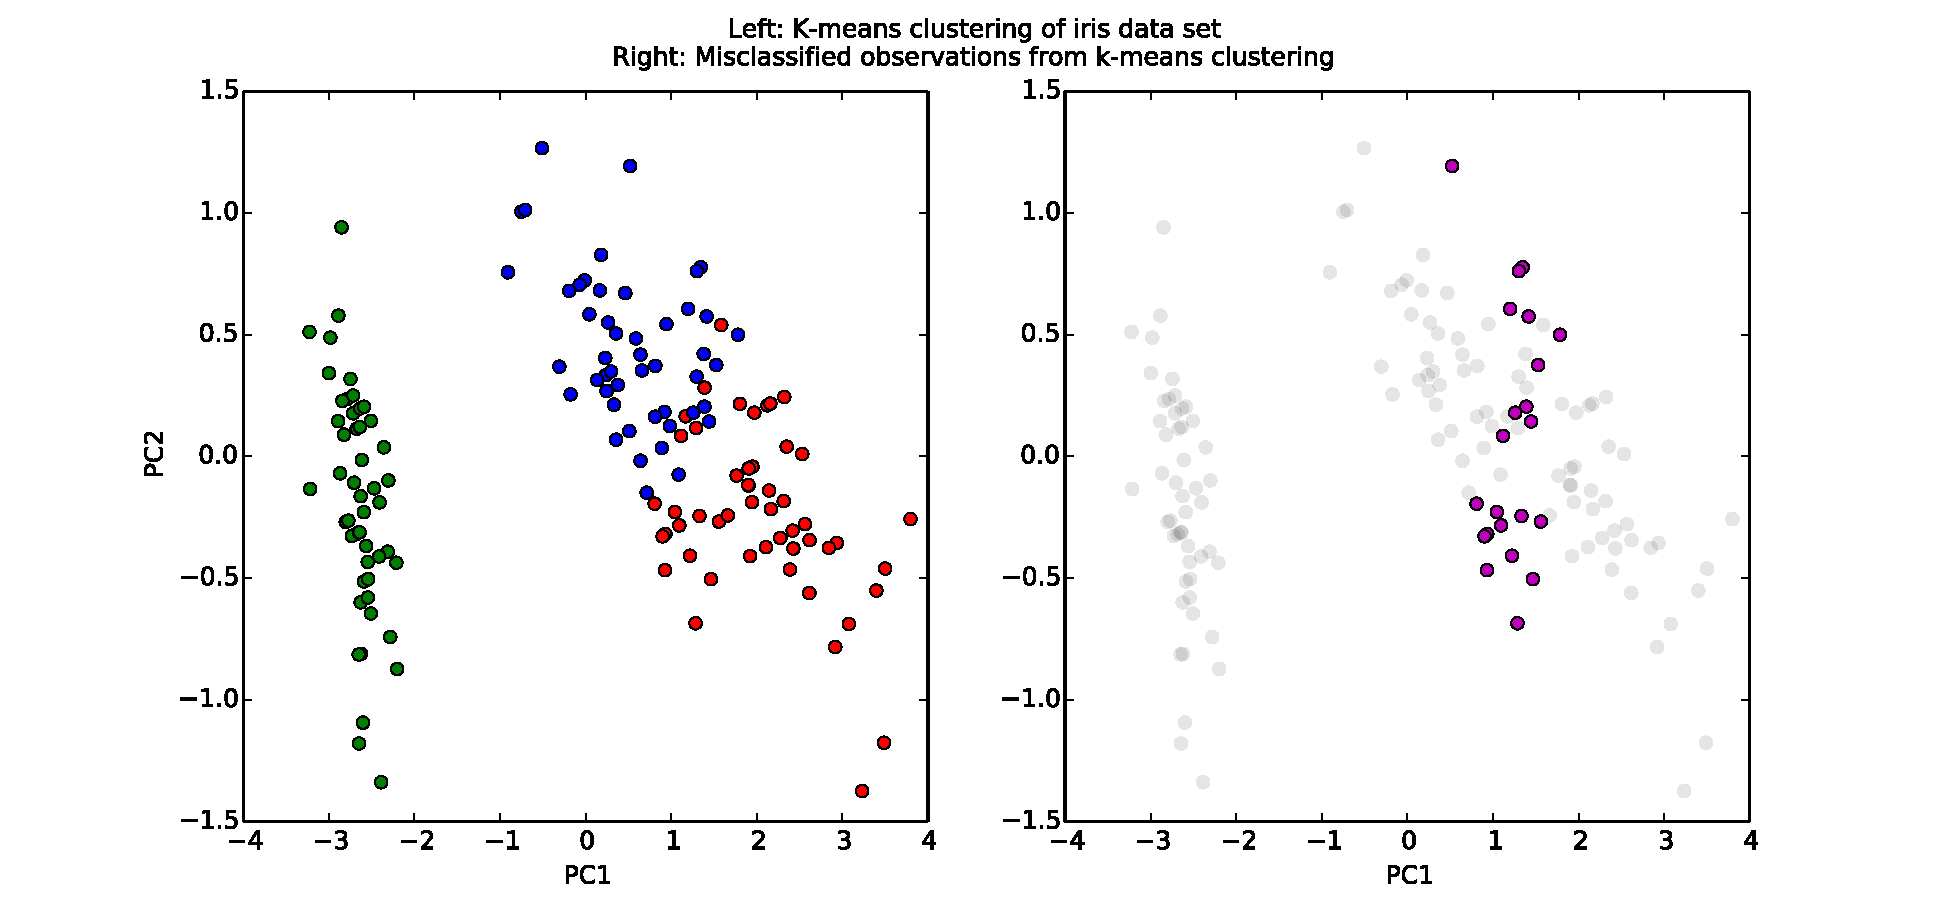
\includegraphics[width=0.9\textwidth]{./figures/hands-on9/fig-python-kmeans.pdf}}
  \caption{Results of applying k-means clustering to the iris data set, using the k-means algorithm impelmented in SciPy.\label{fig:pykmeans}}
\end{figure}


\medskip
\begin{assignment}
\small

Using the `naive' k-means clustering algorithm described in lecture, implement your own k-means clustering function in either Python or R.

Your function should take as input:
\begin{enumerate}
\item A distance matrix
\item an integer, $k$, giving the number of clusters
\item an integer, \verb|maxiter|, giving the maximum number of iterations of the algorithm to perform. NOTE: \verb|maxiter| is an upper limit; you might a choose other criteria for the algorithm to converge, but \verb|maxiter| will guarantee that it completes.
\end{enumerate}

Illustrate your function with application to a data set of your choice.


\end{assignment}

% \section{Minimum Spanning Tree in R}

% The package \texttt{ape} has an \texttt{mst()} function. Several others packages, including vegan also have minimum spanning tree functions. The |mst()| function takes a dissimilarity matrix as its input and returns a square adjacency matrix, $A$, where $A_{ij} = 1$ if $(i,j)$ is an edge in the MST or 0 otherwise.

% Here's an application of the MST function to the cities example you completed above.

% \begin{R}
% > library(ape) # install ape first if necessary
% > city.mst <- mst(as.dist(cities))
% > city.mst # see the adjacency matrix return by mst
% \end{R}

% If you want to create a nice looking plot you can use the  |mat2listw()| function in the package |spdep|. |mat2listw|  converts the adjacency matrix into a form that you can extract the neighbor information from:

% \begin{R}
% > library(spdep) # install spdep first if necessary
% > plot(city.location, type='n', xlab='PCoord1', ylab='PCoord2')
% > text(city.location, labels=names(cities))

% # note British spelling of 'neighbours'
% > plot(mat2listw(city.mst)$neighbours, city.location, add=T) 
% \end{R}







% \chapter{Mixture Modeling and Multidimensional Scaling}
% 

\section{Gaussian Mixture Models in R}

There are multiple packages for fitting mixture models in R.  We'll look at two -- |mixtools| and |MCLUST|.

\subsection{Installing mixtools}

The package |mixtools| can be installed via the GUI or the |install.packages| command. A \href{http://cran.r-project.org/web/packages/mixtools/vignettes/vignette.pdf}{mixtools vignette} can be downloaded from the CRAN website.

\subsection{Using mixtools}

We'll look at how to use mixtools using a data set on eruption times for the Old Faithful geyser in Yellowstone National Park (|?faithful| for details). We'll fit a univariate Gaussian mixture model to the time between eruptions data (\verb|faithful$waiting|).

\begin{R}
# allows us to refer to the variables within waiting time
# without using the standard list "$" syntax
> attach(faithful)

# create a nice histogram
> hist(waiting, main = "Time between Old Faithful eruptions",
xlab = "Minutes", ylab = "", cex.main = 1.5, cex.lab = 1.5, cex.axis = 1.4)

> library(mixtools)
> ?normalmixEM  # read the docs!
> wait.mix <- normalmixEM(waiting)

> names(wait.mix)
[1] "x"          "lambda"     "mu"         "sigma"      "loglik"     "posterior"
[7] "all.loglik" "restarts"   "ft"

# lambda is what we called "pi" in the lecture notes
> wait.mix[c("lambda","mu","sigma")]

> class(wait.mix)
[1] "mixEM"
> ?plot.mixEM  # read about the plotting options for the mixEM object
> plot(wait.mix, density=TRUE)
> plot(wait.mix, loglik=FALSE, density = TRUE, cex.axis = 1.4, cex.lab = 1.4, cex.main = 1.8, main2 = "Time between Old Faithful eruptions", xlab2 = "Minutes")
\end{R}


\begin{figure}[!ht]
    \centering
    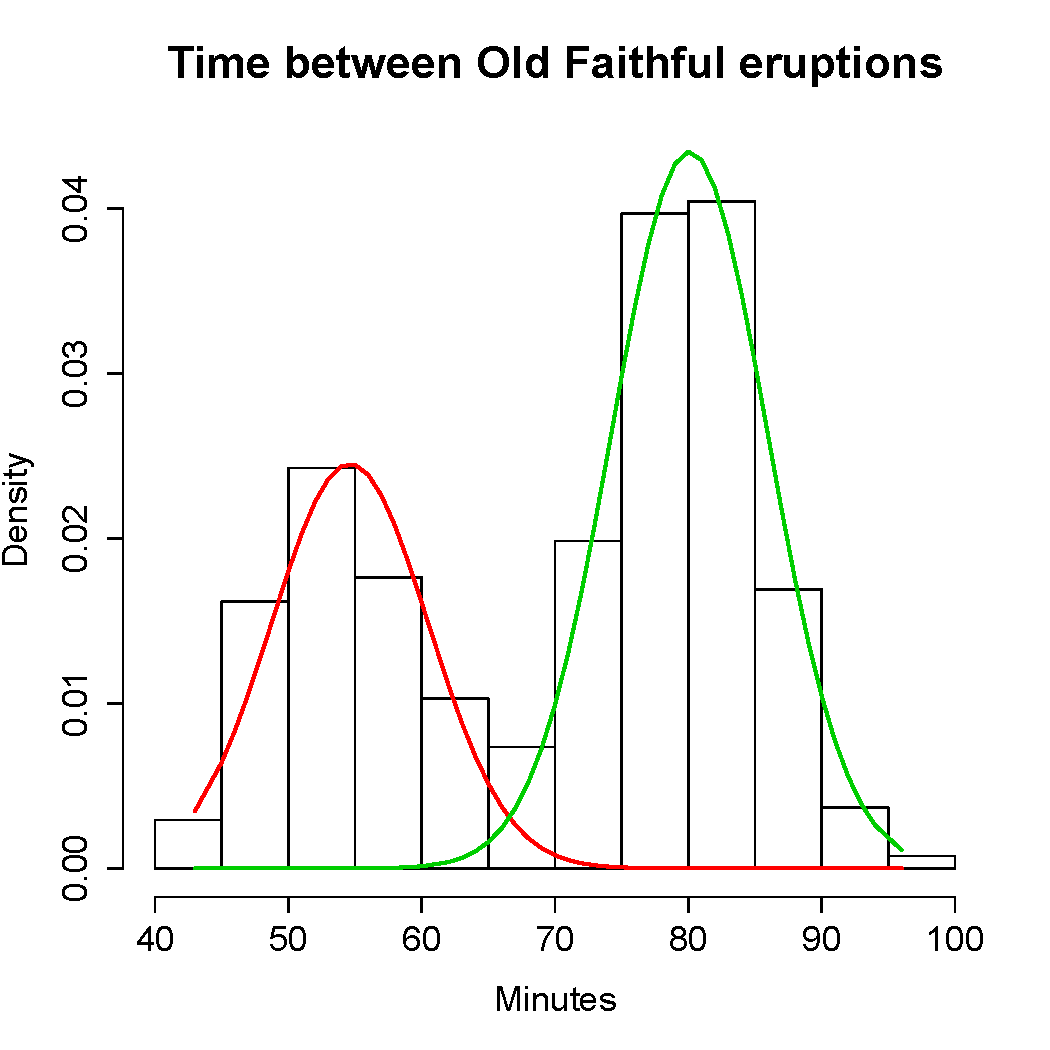
\includegraphics[width=0.5\columnwidth]{./figures/hands-on10/faithful-R.pdf}
    \caption{A Gaussian mixture model for the Old Faithful dataset, estimated using the mixtools module in R.}\label{fig:faithfulR}
\end{figure}


\subsection{Installing MCLUST}
The package |MCLUST| is one of another package that provides maximum likelihood based estimation of mixture models.  You will need to install the package (and it's dependencies) from the R GUI or using the |install.packages| command.

\subsection{Using MCLUST}

We're going to use two data set to illustrate some of |MCLUST|'s capabilities -- the iris data set we've worked with before, and the bivariate version of the Old Faithful data set. We'll start off with  the old faithful data set.

\begin{R}
> plot(faithful$eruptions, faithful$waiting)
\end{R}

From visual inspection of the bivariate scatter plot, it looks like there two clusters. Let's apply the |Mclust| function and see what it suggests:

\begin{R}
> library(mclust)
> fclust <- Mclust(faithful)
> fclust

 best model: elliposidal, equal variance with 3 components
\end{R}

Now that we've running the mixture model, let's look at the results graphically. The following call to |plot| will produce a series of plots.

\begin{R}
> plot(fclust)
\end{R}

The first plot gives is a diagnostic plot that shows the likelihood of the model as a function of  the number of groups (see BIC below). In general, when considering many possible models you want to pick the simplest model that has a highest likelihood. The second graphically represents the classification. The third plots highlights those objects for which the cluster assignment is most uncertain. The fourth plot gives a graphical representation of the Gaussian densities.

The |Mclust| function used a likelihood criterion called the ``Bayesian Information Criterion" (BIC) to estimate the number of components (clusters) in the mixture model. By this criterion it suggested 3 components. BIC, like other information criteria (the Akaike Information Criterion is another popular one), is designed to help choose among parametric models with different numbers of parameters. It tries to choose the simplest model that provides a good fit to the data.

\begin{R}
> names(fclust)
 [1] "modelName"      "n"              "d"              "G"              "BIC"
 [6] "bic"            "loglik"         "parameters"     "z"              "classification"
[11] "uncertainty"
> ?mclust  # check out the docs to read about all the returned parameters
\end{R}

Of course you don't have to accept the number of clusters that the |Mclust| function estimated. Here's how you'd calculate the mixture model with a user determined number of clusters:

\begin{R}
> fclust2 <- Mclust(faithful, G=2)
> plot(fclust2)
\end{R}

% Now let's generate some diagnostic plots for the mixture model:

% \begin{R}
% > plot(fclust)
% \end{R}

If you wanted to generate some of those plots individually you can do the following:

\begin{R}
# generate a plot showing the classifications predicted by mixture model
> mclust2Dplot(data = faithful, what = "classification", identify = TRUE,
    parameters = fclust$parameters, z = fclust$z)
\end{R}

See the docs for the |mclust2Dplot| function for other options.

\subsection{Mixture Models for the Iris data set}

The |MCLUST| package includes the function |clPairs|, a very nice extension of the |pairs| function, for creating scatter plot matrices with group information. The following code illustrates this:

\begin{R}
> names(iris) # remind yourself of the variables in the iris data set
[1] "Sepal.Length" "Sepal.Width"  "Petal.Length" "Petal.Width"  "Species"

# 5th variable is the Species classification
> clPairs(data=iris[,-5], classification=iris[,5])
\end{R}

\begin{figure}[!ht]
    \centering
    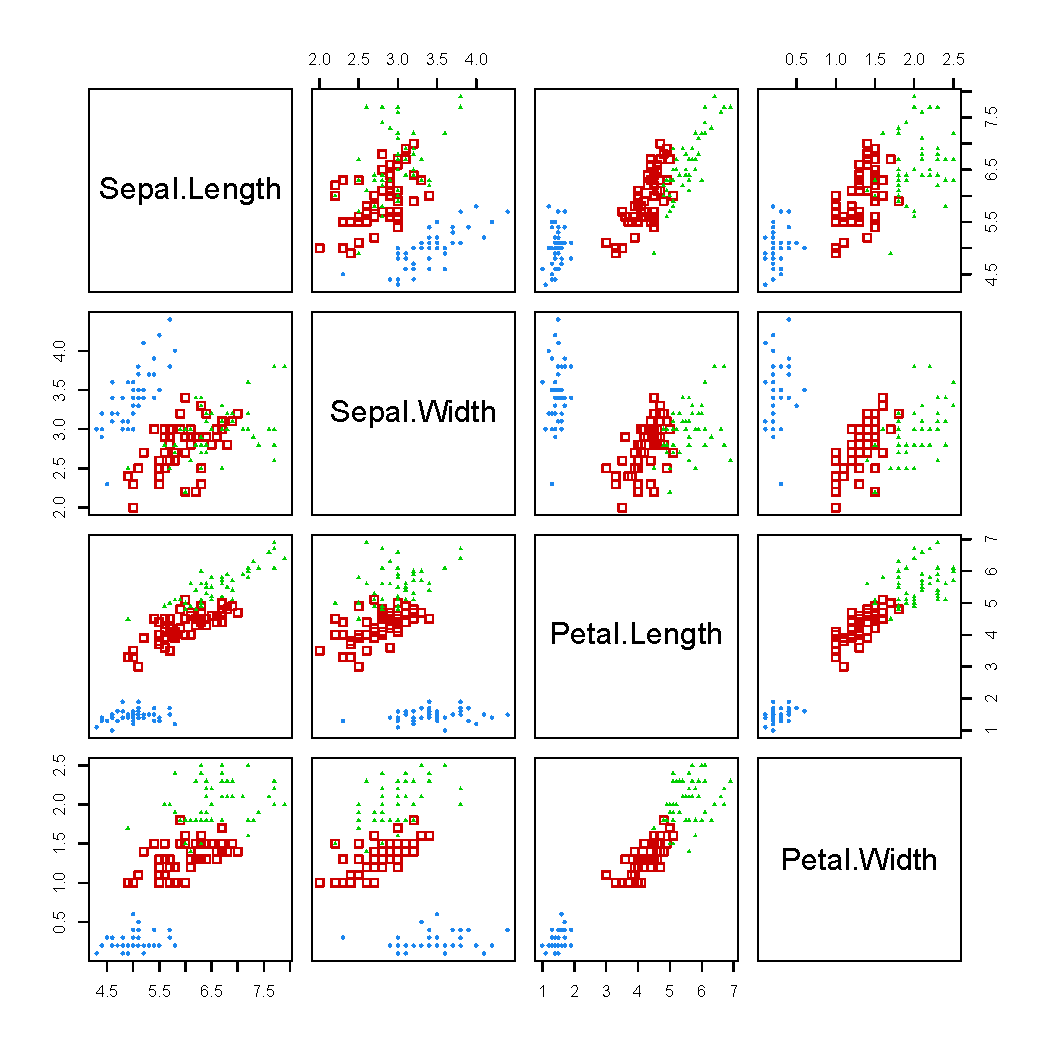
\includegraphics[width=0.5\columnwidth]{./figures/hands-on10/iris-clpairs.pdf}
    \caption{Output of the \texttt{clpairs} function for the iris data set.}\label{fig:clpairs}
\end{figure}

Let's see what |Mclust| makes of the iris data set:

\begin{R}
> iclust <- Mclust(iris[,-5])
> iclust

 best model: ellipsoidal, equal shape with 2 components
> plot(iclust)
\end{R}

Blind to the actual group structure the BIC suggests just two components, whereas we know there are three groups (though \textit{I. versicolor} is thought to be an allopolyploid hybrid; see Kim et al. (2007) Ann Bot, 100: 219-224. ). Examine the first graph produced by the |plot| call above to see how the 2 and 3 component models compare with respect to the BIC.

Now let's see how the mixture model does when we give it the true number of clusters:

\begin{R}
> iclust3 <- Mclust(iris[,-5], G=3)
> plot(iclust3)
\end{R}

To calculate the classification error rate we can compare the estimated clustering to the "true" (known) classification with the |classError| function (|?classError| for details):

\begin{R}
> classError(iclust3$classification, iris[,5])
$misclassified
[1] 69 71 73 78 84

$errorRate
[1] 0.03333333
\end{R}

The |uncerPlot| command allows us to visualize the uncertainty implied by the mixture model to see how uncertain the model was about the misclassified samples.

\begin{R}
> uncerPlot(iclust3$z, iris[,5])
\end{R}

In the uncertainty plot the vertical lines indicate the misclassified samples. As you can see those tend to be among the observations that the mixture model was most uncertain about with respect to which component they belonged to.


\subsection{More details on MCLUST}

See the \href{http://www.stat.washington.edu/research/reports/2006/tr504.pdf}{MCLUST docs} for in depth discussion of the use of |MCLUST|. The examples illustrated above were drawn from this documentation.


\subsection{Mixture Modeling in Python}

The package \href{http://scikit-learn.org/stable/}{scikit-learn} extends the SciPy library with a number of common machine learning algorithms, including an implementation of Gaussian mixture modeling.  |scikit-learn| is included with the EPD distribution you have already installed. The code below demonstrates how to use |scikit-learn| to carry out mixture modeling.

Before you get started use the the |write.table()| function in R to create a tab-delimited version of the |faithful| dataset (hint: use |"\t"| to specify tabs as the separator character, and dont include row names in the file). If you've properly formatted the file you should be able to open it as follows, and create a histogram:
%
\begin{python}
In [1]: f = np.loadtxt('faithful.txt', skiprows=1)
In [2]: f.shape
Out[2]: (272, 2)
\end{python}
%
Assuming that worked, let's import |scikit-learn| and fit a mixture model:
%
\begin{python}
In [4]: from sklearn import mixture
In [6]: classifier = mixture.GMM(n_components = 2)
In [7]: fit = classifier.fit(f[:,1])

In [22]: fit.means_  # means of the estimated subdistributions
Out[22]:
array([[ 80.12056513],
       [ 54.6623402 ]])

In [23]: fit.covars_  # (co)variances of the estimated substrituions
Out[23]:
array([[ 34.08969904],
       [ 34.95662279]])

In [66]: fit.weights_   #  weighting factors (pi in slides)
Out[66]: array([ 0.63770034,  0.36229966])

In [32]: x = linspace(40, 100, 200) # points at which to evaluate the model

# plot histogram using prob density rather than straight up frequency
In [33]: hist(f[:,1], normed=True, alpha=0.2, color='gray')

# draw the PDFs for the two estimated subdistributions
# notice how we multiply each normal PDF by it's weight

In [63]: plot(x, fit.weights_[0] * normpdf(x, fit.means_[0], sqrt(fit.covars_[0])),color='red')
In [64]: plot(x, fit.weights_[1] * normpdf(x, fit.means_[1], sqrt(fit.covars_[1])),color='blue')
In [73]: xlabel("Waiting Time")
In [74]: ylabel("Density")
In [75]: title("Time between Old Faithful eruptions")
\end{python}

\begin{figure}[!ht]
    \centering
    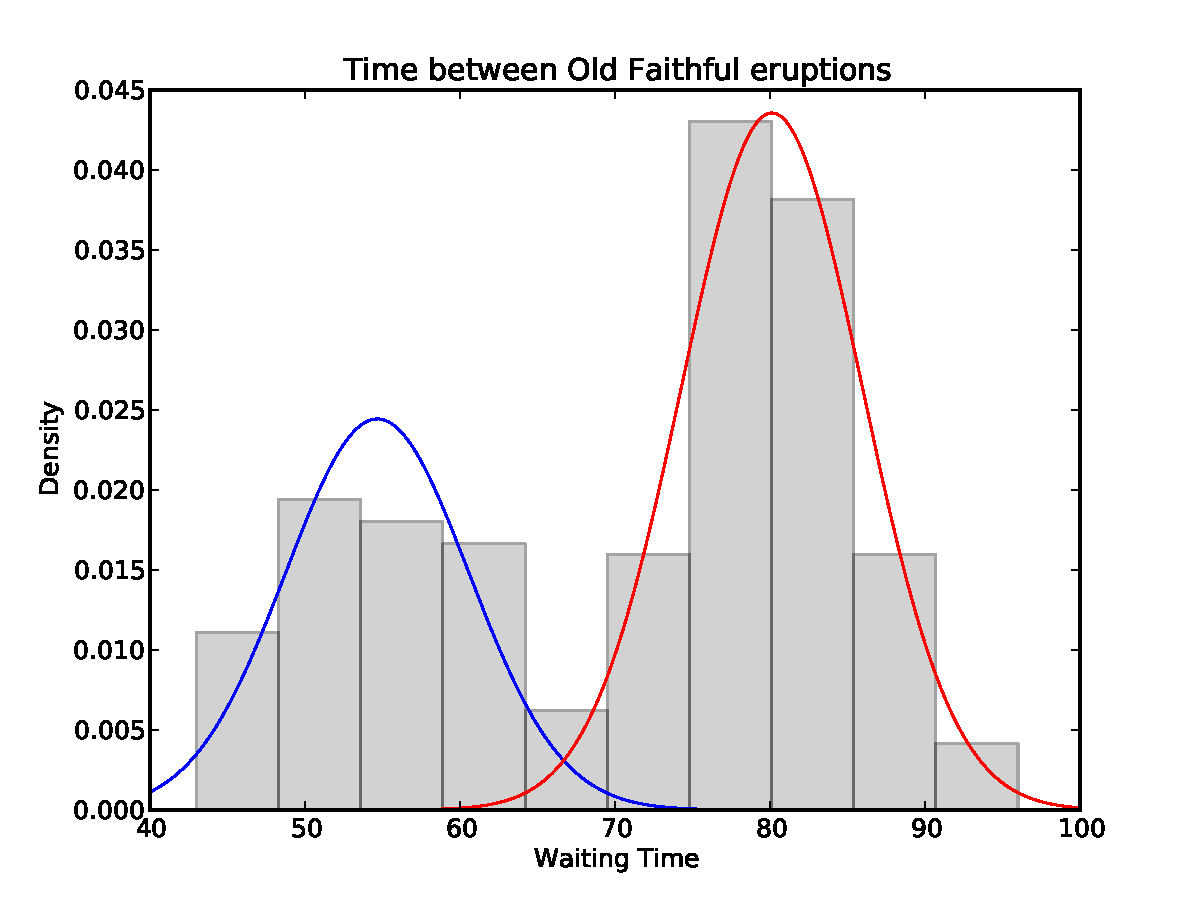
\includegraphics[width=0.5\columnwidth]{./figures/hands-on10/faithful-python.pdf}
    \caption{A Gaussian mixture model for the waiting time variable in the Old Faithful dataset, estimated using the scikit-learn module in Python.}\label{fig:faithfulpy}
\end{figure}

Now let's look at the binary data:
%
\begin{python}
In [4]: plot(f[:,0], f[:,1], 'k.')  # 'k.' gives small black dots as plot points
In [8]: xlabel("Eruption time (mins)")
In [9]: ylabel("Waiting time to next eruption (mins)")

# specify covariance_type = 'full' to estimate complete covariance matrices
In [10]: classifier2 = mixture.GMM(n_components=2, covariance_type='full')
In [11]: fit2 = classifier2.fit(f)

# setup grid to evaluate mixture model over
In [12]: x = linspace(1.5,5,200)
In [13]: y = linspace(40,100,100)
In [14]: X,Y = meshgrid(x, y)
In [23]: XY = np.c_[X.ravel(), Y.ravel()] # like R's c()

# evaluate the mixture model over the grid
In [24]: Z = log(-fit2.eval(XY)[0])
In [25]: Z = Z.reshape(X.shape)
In [26]: cntr = contour(X, Y, Z)
\end{python}
Check out the |scikit-learn| docs for more details and examples.

\begin{figure}[!ht]
    \centering
    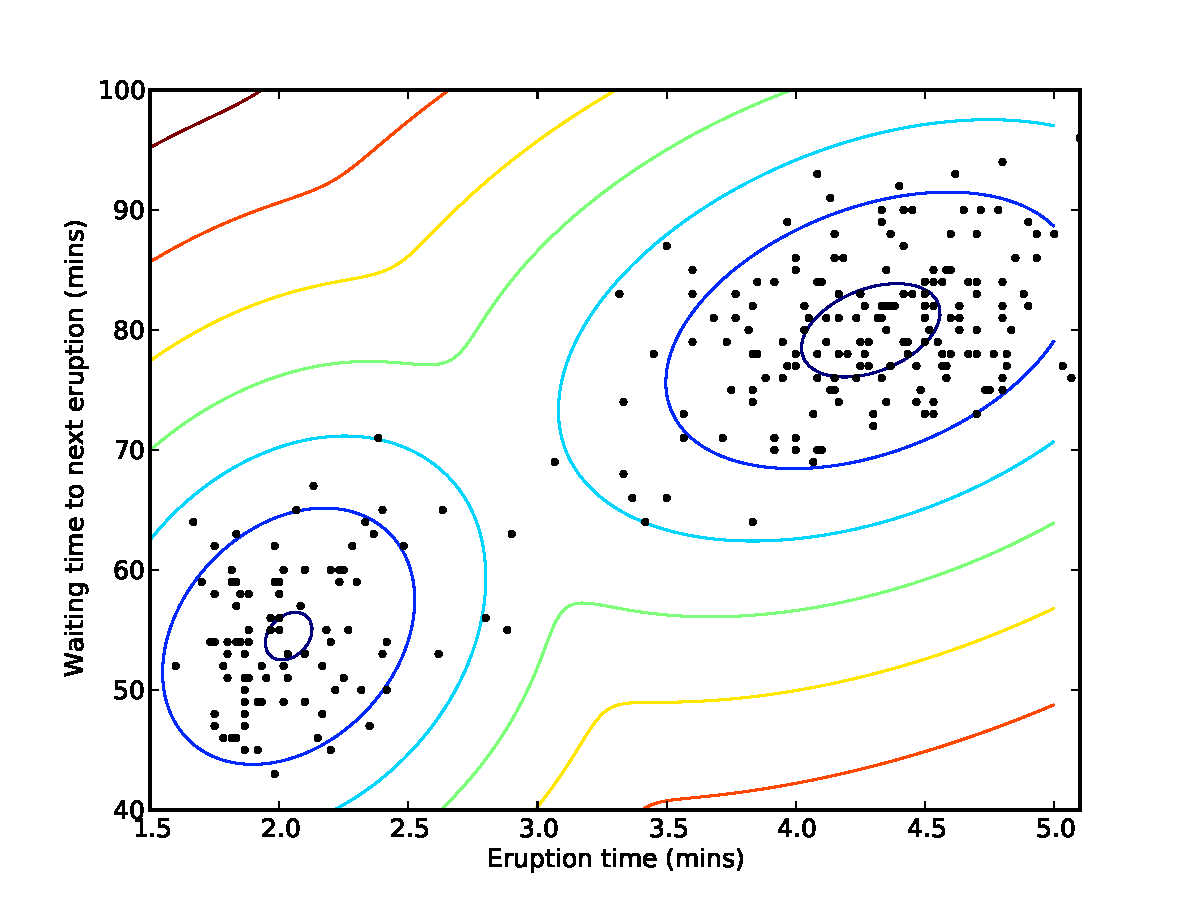
\includegraphics[width=0.5\columnwidth]{./figures/hands-on10/faithful2d-python.pdf}
    \caption{A Gaussian mixture model for 2D Old Faithful dataset, estimated using the scikit-learn module in Python.}\label{fig:faithfulpy2}
\end{figure}


\begin{assignment}
Download the dataset |ddata.txt| from the course wiki. This data set consists of 64 variables measured on 720 specimens. Use the various clustering and ordination techniques you've learned over the course of the semester to explore this data set and estimate the number of clusters in the data.  Use code and figures to support your conclusion.  Hint: you might consider using a lower dimensional approximation of the data to facilitate your analyses.

\end{assignment}


\section{Multidimensional scaling in R}

\subsection{Metric MDS}

The implementation of classic metric scaling in R is carried out using the |cmdscale()| function. Read the documentation for |cmdscale| and then work through the example showing the application of MDS to analysis of road distances between US cities available at the following link (but see notes below first):

\href{http://personality-project.org/r/mds.html}{http://personality-project.org/r/mds.html}.

\medskip
As you work through your example note the following:

\begin{itemize}
\item You can use the |source()| function not only with a local file but also with a URL.  This is convenient but potentially a security issue so don't run code willy nilly without checking out what it does.

\item You can download the code at \href{http://personality-project.org/r/useful.r}{http://personality-project.org/r/useful.r} and check out the functions that it includes. I thought the |read.clipboard()| function was particularly nice.
\end{itemize}





\subsection{Non-metric MDS}

The |isoMDS()| function in the |MASS| package implements the Shepard-Krusal version of non-metric scaling, while the |sammon()| function in the same package use the criterion proposed by Sammon (1969). You will need to utilize these functions, along with |cmdscale| and the hierarchical clustering functions covered last week for the following assignment.

\medskip
\begin{assignment}
Harding and Sokal (1998; PNAS 85:9370-9372; see course wiki) used cluster analysis and non-metric MDS to explore the relationship between European language families as measured by genetic distances among the people who speak those languages.  The classification they derived at large reflects geographic proximity but there are some language families that have distant genetic relationships to their geographic neighbors.

\medskip
Harding and Sokal provide a table of genetic distances that they used in their analyses. Use R to reconstruct the cluster analysis they report (Fig. 1) and repeat this analysis using neighbor joining. In a similar manner use both metric scaling and the Shepard-Kruskal and Sammon criteria for non-metric scaling to do an MDS analysis (similar to Harding and Sokal's fig. 2).  Try to also recreated the MST shown in their figure 2.

\medskip
Submit your code as an R markdown document, and include a brief paragraph describing what differences, if any, you found in your re-analysis of Harding and Sokal data. Are these differences significant (i.e. do they change your interpretation of the data)?

\end{assignment}





% \chapter{Randomization, Boostrap, and LOESS}
% 

\section{Randomization Tests in R}


There are a number of packages (e.g. |coin|) that include functions for carrying out randomization/permutation tests in R. However, it's often just as easy to write a quick set of functions to carry out such tests yourself. We'll illustrate a simple example of this using the ``jackal" example from Manly (2006).

Consider the following data set composed of measures of mandible lengths (in mm) for male and female golden jackals. This set of measurements was taken from a set of skeletons in the collections of the British Museum of Natural History.

\begin{center}
\begin{tabular}{lrrrrrrrrrr}
\hline
Males & 120 & 107 & 110 & 116 & 114 & 111 & 113 & 117 & 114 & 112 \\
Females & 110 & 111 & 107 & 108 & 110 & 105 & 107 & 106 & 111 & 111\\
\hline
\end{tabular}
\end{center}

Let's first create two vectors to represent this set of measurements and create a quick beanplot to visually compare the distributions.

\begin{R}
> males <- c(120,107,110,116,114,111,113,117,114,112)
> females <- c(110,111,107,108,110,105,107,106,111,111)
> library(beanplot)
> beanplot(males,females,side='b',col=list('blue','pink'),names=c("Male","Female"))
> mean(males)
[1] 113.4
> mean(females)
[1] 108.6
> mean(males) - mean(females)
[1] 4.8
\end{R}

The hypothesis we want to test is that male jackals have, on average, larger mandibles than female jackals. The beanplot we constructed and difference in the means would seem to suggest so but let's carry out some more formal tests. The obvious way to compare this set of measurements would be to carry out a t-test, which is approropriate if the samples are normally distributed with approximately equal variance. We have small samples here, so it's hard to know if the normal distribution holds. Instead we'll use a randomization test to compare the observed difference in the means (4.8) to the distribution of differences we would expect to observe if the labels `male' and `female' were randomly applied to samples of equal size from the data at hand.

Let's create a function that takes a sample and randomly assigns the observations to two groups of a specified size. The function takes as input a vector of values (size $N$) and two integers representing the sample sizes ($n_1$ and $n_2$ where $n_1 + n_2 = N$) of the two groups to be compared.

\begin{R}
two.group <- function(x,n1,n2){
  # sample w/out replacement
  reordered <- sample(x, length(x)) # see help(sample) for more info
  g1 <- reordered[seq(1,n1)]
  g2 <- reordered[seq(n1+1,n1+n2)]
  list(g1,g2)
}
\end{R}

Test out this function by calling it repeatedly as shown below. You'll see that it returns a random reordering of the original data, split into two groups:

\begin{R}
> jackals <- c(males,females)
> two.group(jackals,10,10)
# ... output not shown ...
> two.group(jackals,10,10) # call it again to get a different sample
# ... output not shown ...
\end{R}

Now let's write a simple function that returns the mean difference between two samples:

\begin{R}
mean.diff <- function(x1,x2) {
  mean(x1) - mean(x2)
}
\end{R}

Now let's write a generic randomization function:

\begin{R}
randomization <- function(x1,x2,fxn,nsamples=100){
  stats <- c()
  orig <- c(x1,x2)
  for (i in 1:nsamples){
    g <- two.group(orig, length(x1), length(x2))
    stats <- c(stats, fxn(g[[1]],g[[2]]))
  }
  return (stats)
}
\end{R}

We can then use the |randomization| function we wrote as follows to evaluate the signficance of the observed difference in means in the original sample:

\begin{R}
# generate 1000  samples of the mean.diff for randomized data
> rsample <- randomization(males,females,mean.diff,1000)
> hist(rsample)  # examine the distribution

# in how many of the random samples is mean difference between the two groups
# as great or larger than the observed difference in our original samples?
# you might get a slightly different answer
> sum(rsample >= 4.8)
[1] 2
\end{R}

So our conclusion is that the probability of getting a mean difference between samples of this size is about $2/1000=0.002$.  Note that we can't generalize this to golden jackals as a whole because we know nothing about whether these samples actually represent random samples of the golden jackal population or biases that might have been imposed on the collection (e.g. maybe the collectors liked to single out particularly large males). However, if we saw a similar trend (males larger than females) in multiple museum collections we might see this as supporting evidence that the trend held true in general.

Note that we wrote our |randomization| function to take an arbitrary function that takes as it's input two vectors of data. That means we can use it to estimate the randomized distribution of arbitrary statistics of interest. Here we illustrate that with a function that calculates the ratio of variances.

\begin{R}
ratio.var <- function(x1,x2){
    var(x1)/var(x2)
}

> ratio.var(males,females)  # ratio of variances for the original samples
[1] 2.681034
> vsample <- randomization(males,females,ratio.var, 1000)
> hist(vsample)
> mean(vsample)
[1] 1.266088
> sum(vsample >= 2.68)
[1] 74
> 74/1000.
[1] 0.074
\end{R}

In this case the observed ratio of variances isn't particularly unusual.  Let's make one more comparison. We know (or at least we should know!) that ratios of variances have an $F$-distribution so let's compare the distribution of ratios of variances from our randomized sample to that of a sample of the same size drawn from the $F$-distribution with the same degrees of freedom.

\begin{R}
> randomF <- rf(1000, 9, 9) # see help(rf)
> plot(density(vsample),type='l',xlab="Ratio of variances", main="Ratio of Variances\n Theoretical (red) vs Randomization Estimate (black)")
> lines(density(randomF),col='red')
\end{R}


\section{Jackknifing in R}

Jackknife estimates of simple statistics are also relatively straightforward to calculate in R. Here's an example of a simple jackknife function:

\begin{R}
jknife <- function(x, fxn, ci=0.95) {
    theta <- fxn(x)
    n <- length(x)
    partials <- rep(0,n)
    for (i in 1:n){
       partials[i] <- fxn(x[-i])
    }
    pseudos <- (n*theta) - (n-1)*partials
    jack.est <- mean(pseudos)
    jack.se <- sqrt(var(pseudos)/n)
    alpha = 1-ci
    CI <- qt(alpha/2,n-1,lower.tail=FALSE)*jack.se
    jack.ci <- c(jack.est - CI, jack.est + CI)
    list(est=jack.est, se=jack.se, ci=jack.ci)
}
\end{R}

The |bootstrap| package (install if necessary) contains a very similar implementation of a jackknife function (|jackknife()|).

Let's illustrate our jackknife function using samples drawn from a Poisson distribution. The Poisson is a discrete probability distribution that is often used to describe the probability of a number of events occuring in a fixed period of time, where the events are independent and occur with an average rate $\lambda$. The Poisson distribution is used to model processes like mutations in DNA sequences or atomic decay.  Both the mean and variance of a Poisson distribution are equal to $\lambda$. Let's see how well the jackknife does at estimating confidence intervals for  the mean and variance of a modest number of samples drawn from a Poisson.

\begin{R}
> psample <- rpois(25,4) # 25 obsevations from poisson with lambda = 4
> psample  # your sample will be different
 [1] 3 1 1 3 3 3 5 4 1 4 6 5 6 3 4 5 6 1 1 2 3 7 3 4 5
> mean(psample)
[1] 3.56
> var(psample)
[1] 3.173333
> jknife(psample, mean)$ci
[1] 2.824680 4.295320
> jknife(psample, var)$ci
[1] 1.716397 4.630270
\end{R}

In both cases above, the true mean and variance were contained within the 95\% confidence intervals estimated by the jackknife. Let's do a little experiment to see how often that's true for samples of this size:

\begin{R}
# create 500 samples of size 25 drawn from Poisson w/lambda=4
> psamples <- matrix(rpois(25*500,4),ncol=25,byrow=T)
> dim(psamples)
[1] 500  25

# create a convenience function
> get.ci <- function(x) { return(x$ci) }  #x$ci gives confidence interval

# generate jackknife estimates for mean
> j.mean <- apply(psamples, 1, jknife, mean)

# make matrix that holds 95% confidence intervals of mean
> mean.ci <- t(sapply(j.mean, get.ci))
> mean.ci[1,]
[1] 2.796265 4.323735
> mean.ci[2,]
[1] 3.562991 4.917009

# check how often true mean is w/in CI
> sum(mean.ci[,1] <=4 & mean.ci[,2] >= 4)
[1] 463
> 463/500
[1] 0.926
# true mean is w/in estimated 95% CI about 93% of the time.

# now the same for variances
> j.var <- apply(psamples, 1, jknife, var)
> var.ci <- t(sapply(j.var, get.ci))
> sum(var.ci[,1] <=4 & var.ci[,2] >= 4)
[1] 449
> 449/500.
[1] 0.898
# true variance is w/in 95% CI only 90% of time
\end{R}


In the case  of the confidence intervals for the mean, the jacknife estimator did a decent job -- the true mean is with the 95\% confidence interval about 93\% of the time.  In the case of the variance it did less well.  The jackknife confidence intervals work well when the estimator is normally distributed. This suggests that one way we might improve the jackknife CIs is by using a normalizing transformation, like the logarithm function:

\begin{R}
> log.var <- function(x){log(var(x))}
> j.log.var <- apply(psamples, 1, jknife, log.var)
> log.var.ci <- t(sapply(j.log.var, get.ci))
> sum(log.var.ci[,1] <=log(4) & log.var.ci[,2] >= log(4))
[1] 472
> 472/500.
[1] 0.944
# a substantial improvement in the performance of the 95% CIs
\end{R}

This illustrates the type of simulation study you might do to check the robustness of the jackknife for a statistic of interest for a given class of distributions.

\section{Bootstrapping in R}

There are several packages that provide functions for doing bootstrapping in R. These include |bootstrap| and |boot|. We'll take a quick look at the functions in |bootstrap|. Install |bootstrap| using the standard package installation mechanism.

We'll use the same set of samples from the Poisson that we used before to illustrate the jackknife.
%
\begin{R}
> library(bootstrap)
> ?bootstrap  # as always, check out the docs
# generate 1000 bootstrap sample estiamte of var
> b <- bootstrap(psample, 1000, var)

# standard bootstrap confidence limits
# based on assumption of normality
> bstar <- b$thetastar
> c(mean(bstar)-1.96*sd(bstar), mean(bstar)+1.96*sd(bstar))
[1] 1.774923 4.348151

# estimate the bootstrap percentile confidence limits
> quantile(b$thetastar,c(0.025,0.975))
    2.5%    97.5%
1.839583 4.373333

# for comparison remind ourself of what the jackknife CI was
> jknife(psample,var)$ci
[1] 1.716397 4.630270
\end{R}
%

% Now let's use the bootstrap to look at the distribution of a more complicated statistic -- the fraction of the variance explained by the first principal component.  To do this, first we need to define a function that return the statistic we're interested in:
% %
% \begin{R}
% > pca.1stpc.ratio <- function(x){
% +    x.pca <- prcomp(x, center=T, scale.=T)
% +    pca.var <- x.pca$sdev**2
% +    return (pca.var[1]/sum(pca.var))
% + }
% \end{R}
% %
% Having defined this function we can generate bootstrap samples to estimate the distribution of this statistic:
% %
% \begin{R}
% > iris.sub <- subset(iris, select=

% \end{R}

\section{LOESS Models}

LOESS (aka LOWESS; `Locally weighted scatterplot smoothing') is a
modeling technique that fits a curve (or surface) to a set of data using
a large number of local regressions. Local weighted regressions are fit
at numerous regions across the data range, using a weighting function
that drops off as you move away from the center of the fitting region
(hence the `local' aspect). LOESS combines the simplicity of least
squares fitting with the flexibility of non-linear techniques and
doesn't require the user to specify a functional form ahead of time in
order to fit the model. It does however require relatively dense
sampling in order to produce robust fits.

Formally, at each point $x_i$ we estimate the regression coefficients
$\hat{\beta}_j(x)$ as the values that minimize:
\[\sum_{k=1}^n w_k(x_i)(y_k - \beta_0 - \beta_1 x_k - \ldots - \beta_d x_k^2)^2\]
where $d$ is the degree of the polynomial (usually 1 or 2) and $w_k$ is
a weight function. The most common choice of weighting function is
called the ``tri-cube'' function which is defined as:

\lstDeleteShortInline|
\begin{align*}
 w(x) & = (1-|x|^3)^3, \mbox{for}\ |x| < 1  \\
      & = 0,\ \mbox{for}\ |x| \geq 1
\end{align*}
\lstMakeShortInline|


% \medskip
% \begin{assignment}
% Write an R function that computes the tri-cube
% function described above. Create a plot of the tri-cube function over
% the interval (-3,3). Create a second R function that calculates the
% Gaussian function $f(x) = e^{-x^2}$ and plot that function over the same
% interval, in the same plot, to compare the two functions.  Make sure you use a suitably dense sampling of points to get an accurate assesment of the shape of each function.
% \end{assignment}

The primary parameter that a user must decide on when using LOESS is the
size of the neighborhood function to apply (i.e.~over what distance
should the weight function drop to zero). This is referred to as the
``span'' in the R documentation, or as the parameter $\alpha$ in many of
the papers that discuss LOESS. The appropriate span can be determined by
experimentation or, more rigorously by cross-validation.

We'll illustrate fitting a LOESS model using data on Barack Obama's
approval ratings over the period from Jan 2007 to November 2012, using data downloaded from \url{pollster.com}. This data is available as  \lstinline!obama-favorable-rating.csv! on the class wiki.
%
\begin{R}
> polls <- read.csv('obama-favorable-rating.csv')
> names(polls)
 [1] "Pollster"               "Start.Date"             "End.Date"
 [4] "Release.Date.Time..ET." "Number.of.Observations" "Population"
 [7] "Mode"                   "Favorable"              "Unfavorable"
[10] "Undecided"              "Pollster.URL"           "Source.URL"
[13] "Source.URL.1"
> dim(polls)
[1] 666  13
# polls are in reverse chronological order so let's reverse them
# so we can look at trend from earliest to most recent dates
> fav <- rev(polls$Favorable)
> pollnum <- 1:length(fav)
> plot(pollnum, fav,pch=16, cex=0.5,col='grey')
> loess.fav <- loess(fav ~ pollnum)
> pred.fav <- predict(loess.fav, pollnum)
> lines(pollnum, pred.fav, lwd=2, col='red')

# now with a smaller neighborhood span
> loess.fav2 <- loess(fav ~ pollnum, span=0.25)
> pred.fav2 <- predict(loess.fav2, pollnum)
> lines(pollnum, pred.fav2, lwd=2, col='blue')
\end{R}
Take note of how the LOESS curve changed when we made the span smaller.
By decreasing the span we've increased the sensitivity of the model
(perhaps overfitting in this case).

\medskip
\begin{assignment}
Write an R function that genereates a plot that
simultaneously illustrates trends in both approval and disapproval
ratings for Barack Obama, showing both the raw data and corresponding
LOESS fits. Use colors and/or shapes to distinguish the two trends. Make
sure both your x- and y-axes are scaled to show the full range of the
data. Label your axes and create a title in the plot. Aim for a
`publication quality' figure.
\end{assignment}



% \chapter{Simulating Gene Networks}
% 
\section{Key Elements of the Model}


We're going to build a simple model of gene regulation using a `logic approximation' where gene expression is either on or off.  When a gene, $Y$ is being transcribed it is produced at a rate $\beta$, and is being degraded at a rate proportional to the amount transcript, $\alpha Y$. A differential equation to describe the change of $Y$ over time is:
\[
\frac{dY}{dt} = \beta - \alpha Y
\]
%
This represents an instantaneous rate of change of $Y$. We'll implement this with a simple Python function, that we'll call |update()|
%
\begin{python}
def update(ynow, alpha, beta):
    delta = beta - alpha * ynow
    return ynow + delta
\end{python}
%

For our first exploration, we'll assume that $Y$ is turned on immediately at the start of our simulation, and transcription is never turned off.
%
\begin{python}
t = range(100)  # 100 ticks of the clock
alpha, beta = 0.1, 0.1
ynow = 0  # initialize y to zero
ys = [ynow] # we'll keep track of y vals

for tick in t[1:]:
    ynew = update(ynow, alpha, beta)
    ys.append(ynew)
    ynow = ynew

plot(t, ys)
ylim(0,2)
\end{python}
%
\begin{figure}[!ht]
    \centering
    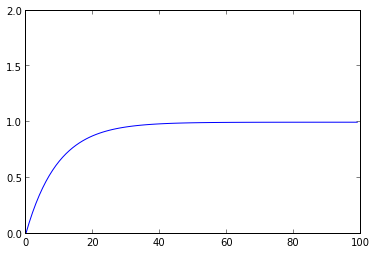
\includegraphics[width=0.33\columnwidth]{./figures/hands-on12/fig-simpleon.png}
    \caption{Expression of gene $Y$ after induction at time $t=0$.}\label{fig:simpleon}
\end{figure}
%
Your output should look like Fig.~\ref{fig:simpleon}. Notice that $Y$ reaches a steady state, $Y_{st} = \beta/\alpha$.  Take a few minutes to re-run the above code with different values of $\alpha$ and $\beta$ to understand how these two parameters interact.


Now let's put the regulation of $Y$ under the control of an external signal, $X$. When $X$ reaches a threshold $k_x$, $Y$ is transcribed. When $X$ is under this threshold, transcription of $Y$ ceases. We will make $X$ a pulse like signal, so let's write a function to generate pulses:
%
\begin{python}
def pulse(ontime, offtime,  ntimes=100, onval=1):
    signal = np.zeros(ntimes)
    signal[ontime:offtime] = onval
    return signal
\end{python}
%
And use the pulse function as follows:
%
xs = pulse(20, 80, 120)
plot(xs)
ylim(0,2)
%
Now let's update our simple simulation so $Y$ responds to $X$:
%
\begin{python}
xs = pulse(20,80,120)
alpha, beta = 0.1, 0.1
kx = 0.5
ynow = 0
ys = []
for x in xs:
    tbeta = 0
    if x > kx:
        tbeta = beta
    ynew = update(ynow, alpha, tbeta)
    ys.append(ynew)
    ynow = ynew

p1, = plot(xs)
p2, = plot(ys)
legend([p1,p2],["X","Y"])
xlabel("time")
ylim(0,2)
\end{python}
%
\begin{figure}[!ht]
    \centering
    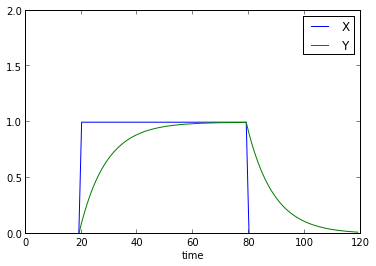
\includegraphics[width=0.33\columnwidth]{./figures/hands-on12/fig-pulse.png}
    \caption{Expression of gene $Y$ under control of signal $X$.}\label{fig:pulse}
\end{figure}
%
And now let's wrap this logic up into a simple function:
%
\begin{python}
def simplereg(xs, alpha, beta, kx, yinit=0):
    ynow = yinit
    ys = []
    for x in xs:
        talpha = alpha
        tbeta = 0
        if x > kx:
            tbeta = beta
        ynew = update(ynow, talpha, tbeta)
        ys.append(ynew)
        ynow = ynew
    return ys

\end{python}
%
We can then call this function as:
%
\begin{python}
xs = pulse(20,80,120)
ys = simplereg(xs, 0.1, 0.1, 0.5)
p1, = plot(xs)
p2, = plot(ys)
legend([p1,p2],["X","Y"])
xlabel("time")
ylim(0,2)
\end{python}
This should generate a figure identical to our previous one.

\section{Autoregulation}

Now that we've got a simple simulation working, let's get a little fancier. We'll implement a model where $Y$ negative regulates it's own transcript levels. This time we'll dive write into writing a simle function to represent the negative autoregulation case:
%
\begin{python}
def autoreg(xs, alpha, beta, kx, alphaneg, ky, yinit=0):
    ynow = yinit
    ys = []
    for x in xs:
        talpha = alpha
        tbeta = 0
        if x > kx:
            tbeta = beta
        if y > ky:
            talpha = alphaneg
        ynew = update(ynow, talpha, tbeta)
        ys.append(ynew)
        ynow = ynew
    return ys
\end{python}
%
This function is almost identical to our simple regulation case, except now we check to see if $Y$ is above it's own threshold for autoregulation. If so we increase the rate of decay. We can put this |autoreg| function to work as so:
%
\begin{python}
xs = pulse(20,80,120)
ys = simplereg(xs, 0.1, 0.1, 0.5)
yneg = autoreg(xs, 0.1, 0.1, 0.5, 0.2, 0.25)

p1, = plot(xs)
p2, = plot(ys)
p3, = plot(yneg)
legend([p1,p2,p3],["$X$","$Y$","$Y_{neg}$"])
xlabel("time")
ylim(0,2)
\end{python}

We see that with negative autoregulation, $Y$ comes to a lower steady state, but also that it reaches steady state quicker than in the simple on case. It is typical to refer to the response time of a systems as the time it takes to reach one-half it's steady state value.  As we discussed in the lecture, this time is purely a function of the degradation rate, $T_{1/2} = \log(2)/\alpha$.

Negative autoregulation, when coupled with a higher rate of transcription, can be used to reach a similar steady state more quickly as shown below:
%
\begin{python}
xs = pulse(20,80,120)
ys = simplereg(xs, 0.1, 0.1, 0.5)
yneg = autoreg(xs, 0.1, 0.2, 0.5, 0.2, 0.25) # note change in 3rd argument (beta)

p1, = plot(xs)
p2, = plot(ys)
p3, = plot(yneg)
legend([p1,p2,p3],["$X$","$Y$","$Y_{neg}$"])
xlabel("time")
ylim(0,2)
\end{python}

We can use the very same |autoreg| function to implement positive autoregulation, as follows:
%
\begin{python}
xs = pulse(20,80,120)
ys = simplereg(xs, 0.1, 0.1, 0.5)
yneg = autoreg(xs, 0.1, 0.2, 0.5, 0.2, 0.25)
ypos = autoreg(xs, 0.1, 0.05, 0.5, 0.05, 0.25) # note change in 3rd and 5th args

p1, = plot(xs, lw=0.5)
p2, = plot(ys, lw=2)
p3, = plot(yneg, lw=2, ls='dashed')
p4, = plot(ypos, lw=2, ls='dashed')

legend([p1,p2,p3,p4],["$X$","$Y$","$Y_{neg}$","$Y_{pos}$"])
xlabel("time")
ylim(0,2)
\end{python}
%
\begin{figure}[!ht]
    \centering
    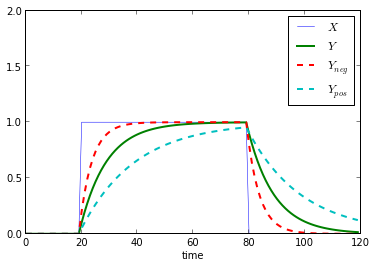
\includegraphics[width=0.33\columnwidth]{./figures/hands-on12/fig-autoreg.png}
    \caption{Contrasting simple regulation, negative autoregulation, and positive autoregulation.}\label{fig:autoreg}
\end{figure}


\section{Feed-forward Loops}

Let's add another gene, $Z$, to our network. We'll start by examing the behavior of a type of network topology (motif) called a `feed-forward loop' (FFL).


\subsection{Coherent FFLs}
The first FFL we'll examine is a `coherent FFL' -- coherent because both the short-arm (directly from $X$ to $Z$) and long-arms of the loop (with $Y$ as an intermediate) have the same effect on $Z$. In this first example, we will implement a coherent FFL with AND logic.

\begin{figure}[!ht]
\centering
% \begin{dot2tex}[options=-tmath]
% digraph G {
%     graph [rankdir=LR];
%     node [shape="circle"];
%     edge [style="-triangle 90"];
%     X -> Y -> Z;
%     X -> Z;
%     }
% \end{dot2tex}
\begin{tikzpicture}[node distance=2cm, auto,>=triangle 45]
  \node (X) {$X$};
  \node [right of=X] (Y) {$Y$};
  \node [right of=Y] (Z) {$Z$};
  \draw[->] (X) --  (Y);
  \draw[->] (Y) -- (Z);
  \draw[->] (X) to [bend right=30] (Z);
\end{tikzpicture}
\caption{A coherent FFL.}
\end{figure}
%
\begin{python}
def coh_ffl_and(xs, yalpha=0.1, ybeta=0.1, kxy=0.5, zalpha=0.1, zbeta=0.1, kxz=0.5, kyz=0.5):
    ynow = 0
    ys = []
    znow = 0
    zs = []
    for x in xs:
        yb = 0
        if x > kxy:
            yb = ybeta
        ynew = update(ynow, yalpha, yb)
        ys.append(ynew)

        zb = 0
        if (x > kxz) and (ynow > kyz):
            zb = zbeta
        znew = update(znow, zalpha, zb)
        zs.append(znew)

        ynow = ynew
        znow = znew
    return ys, zs
\end{python}
%
And we'll test our function with the following code:
%
\begin{python}
xs = pulse(10,15,120) + pulse(40,100,120)
ys, zs = coh_ffl_and(xs, kyz=0.5)

p1, = plot(xs)
p2, = plot(ys)
p3, = plot(zs)
legend([p1,p2,p3,p4],["$X$","$Y$","$Z$"])
xlabel("time")
ylim(0,2)
\end{python}
%
In the example above, our $X$ signal represents two pulses -- a short pulse starting at time point 10, and a more sustained pulse at time point 40. As suggested by Shen-Orr et al., and illustrated in Fig.~\ref{fig:cohffland}, the coherent FFL motif with AND logic can act as a type of sign-sensitive filter.  $Z$ doesn't turn on until $Y$ reaches a critical threshold, but both $Y$ and $Z$ turn off simultaneously.
%
\begin{figure}[!ht]
    \centering
    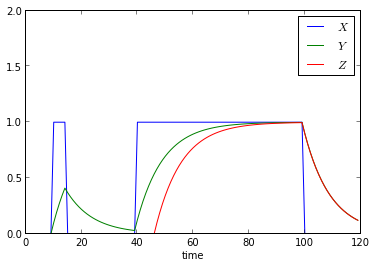
\includegraphics[width=0.33\columnwidth]{./figures/hands-on12/fig-cohffland.png}
    \caption{Behavior of a coherent FFL with AND logic at $Z$.}\label{fig:cohffland}
\end{figure}


Now let's add some random noise to our input signal, $X$.
%
\begin{python}
nxs = xs + np.random.rayleigh(0.5,size=len(xs)) # add some random noise to the signal
nxs = abs(nxs - 0.5)
plot(nxs);
\end{python}
%
Let's see how the noise effects the network:
%
\begin{python}
ys, zs = coh_ffl_and(nxs, kyz=0.5)

p1, = plot(nxs)
p2, = plot(ys)
p3, = plot(zs)
legend([p1,p2,p3,p4],["$X$","$Y$","$Z$"])
xlabel("time")
ylim(0,2)
\end{python}
%
As shown in Fig.~\ref{fig:noisyffl}, $Z$ is effectively buffered from the noise.
%
\begin{figure}[!ht]
    \centering
    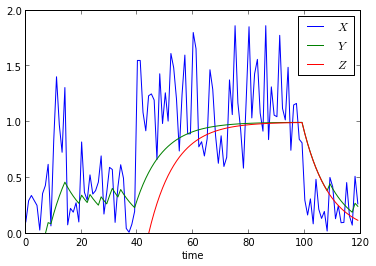
\includegraphics[width=0.33\columnwidth]{./figures/hands-on12/fig-noisyffl.png}
    \caption{Behavior of a coherent FFL with AND logic at $Z$, in response to a noisy input signal $X$.}\label{fig:noisyffl}
\end{figure}

\medskip
\begin{assignment}
Write an Python function that generates a coherent FFL with OR logic at $Z$ (i.e. $Z$ is on if either $X$ or $Y$ are above their respective thresholds), and illustrate this network motif for a variety of parameter settings.  How does the behavior of the coherent FFL with OR logic differ from the similar topology with AND logic?
\end{assignment}


% \chapter{Building a Bioinformatics Pipeline}
% 
\section{Overview}

Building on our initial forays into building bioinformatics pipelines last week, we now turn to a more complicated example that integrates BioPython along with several command line programs.  This pipeline will incorporate such features as web based queries and conversion of information between different file formats.

\section{The Pipeline}


The tasks carried out by the pipeline will be as follows:

\begin{itemize}

\item Read in a nucleotide sequence from a FASTA file
\item Translate the nucleotide sequence to an amino acid sequence
\item Do a blastp search against human and fly proteins in the Swiss-Prot database using an interface to the NCBI web version of BLAST
\item Download protein sequences for the best blast hits from Swiss-Prot
\item Use MAFFT to do a multiple alignment of the original amino acid sequence and the presumed orthologs generated via the blast search
\item Analyze the query protein for known protein domains using HMMER and Pfam
%\item Use a web service to query the KEGG pathways database to look for pathways that include orthologues to your gene of interest

\end{itemize}

\section{Installing Additional Software and Modules}

Before we start building our pipeline, we'll need to install a few additional tools., including the Biopython library, and two commonly used bioinformatics sofware packages called HMMER and MAFFT.  HMMER and MAFFT will be installed at using the system level package manager (Debian's APT system) using the command line tool, aptitude.  Biopython will be installed using the Conda package manager, for managing the Python environment.

\subsection{Installing HMMER}

HMMER is an implementation of a profile Hidden Markov Model (HMM) for protein sequence analysis. You can read up on HMMER at the \href{http://hmmer.janelia.org/}{HMMER website}. We will use it here for finding protein domains in sequences in conjuction with the PFAM database. To install HMMER type the following commands in the Bash shell (\emph{not} from the Python interpreter):
%
\begin{bash}
$ sudo aptitude update # insures the list of packages is up to date
$ sudo aptitude install HMMER 
\end{bash}

\subsubsection{Get the PFAM HMM library}

We will be using the Pfam database (Release 27) in conjunction with HMMER to search for known protein domains in our sequences of interest. To download PFAM, you can use the \verb|curl| command line tool:
%
\begin{code}
$ curl -O ftp://ftp.sanger.ac.uk/pub/databases/Pfam/releases/Pfam27.0/Pfam-A.hmm.gz
\end{code} %$
%
This is a large file (202MB) and decompresses to an even larger file (approx. 1GB). Make sure you have adequate disk space. Once the download completes you can unzip it as follows:
%
\begin{code}
$ gunzip Pfam-A.hmm.gz
\end{code} %$



\subsection{Installing MAFFT}

MAFFT is a multiple sequence alignment program. It's relatively fast and a number of studies have shown that it is amongst the best performing multiple sequence aligners. MAFFT is usually the sequence aligner I reach for first.  Clustalw is the `classic' alignment tool, so it's useful to have on your system, but MAFFT usually gives better alignments (though Clustalw2 is supposed to address some of the short-comings of the older versions of Clustalw). See the \href{http://mafft.cbrc.jp/alignment/software/}{MAFFT website} for additional references and information. 
%
\begin{bash}
$ sudo aptitude install mafft  
\end{bash} %$

\subsection{Installing Biopython}

Biopython is easily installed using the \verb|conda| package manager:
%
\begin{bash}
$ conda install biopython
\end{bash} %$


\section{Biopython}

Now we turn our attention to Biopython.  As we build our pipeline I will first demonstrate the use of various modules, classes, and functions in the interactive shell and then I will give a set of functions that consolidate the commands to make them convenient to use.

\subsection{Test files}

Download the file |unknown1.fas| and |unknown2.fas| from the class website. I recommend you place these in |~/tmp|.

\subsection{Reading in a single sequence from a FASTA file}

Fire up and ipython interpreter, either a text based command line (|ipython --pylab|) or an ipython notebook (|ipython notebook --pylab=inline|).


We'll start by showing how to read sequence data out of a FASTA file:
\begin{python}
>>> cd ~/tmp
>>> from Bio import SeqIO
>>> u1 = SeqIO.read('unknown1.fas','fasta')
>>> type(u1)
<class 'Bio.SeqRecord.SeqRecord'>
>>> u1
SeqRecord(seq=Seq('ATGATGAATTTTTTTACATCAAAATCGTCGAAT
CAGGATACTGGATTTAGCTCT...TGA', SingleLetterAlphabet()),
id='YHR205W', name='YHR205W', description='YHR205W  Chr 8', dbxrefs=[])
>>> u1.name
'YHR205W'
>>> u1.description
'YHR205W  Chr 8'
>>> u1.seq
Seq('ATGATGAATTTTTTTACATCAAAATCGTCGAATCAGGATACTGG
ATTTAGCTCT...TGA', SingleLetterAlphabet())
>>> u1.seq[:10]
Seq('ATGATGAATT', SingleLetterAlphabet())
>>> u1.seq[0]
'A'
>>> u1.seq[9]
'T'
>>> u1.seq[:10].tostring()
'ATGATGAATT'
>>> u1.seq.translate()[:10]
Seq('MMNFFTSKSS', HasStopCodon(ExtendedIUPACProtein(), '*'))
\end{python}

|SeqIO| is a sub-module of the top-level module Biopython module |Bio|.  The function |SeqIO.read()| reads a single sequence object from a file and returns an instance of a |SeqRecord| class (defined in the Biopython package). A \emph{class} is a programming concept that groups data and functions that operate on that data into a single object. For example, in the code above we used the |.name| and |.description| attributes to examine information about the sequence (this information was retrieved from the FASTA file itself).  A |SeqRecord| holds a |Seq| object (yet another class!) as well as accessory information like the name of the sequence, a description, etc. |Seq| objects act very much like strings in terms of slicing and element access but they also have specialized function like |.translate()| that can be used to translate a nucleotide sequence into a peptide sequence.

\subsubsection{Reading in multiple sequences from a FASTA file}

In the code above we demonstrated how to read a single sequence from a FASTA file.  Here we demonstrate how to read multiple sequences.  The key difference is the use of the |SeqIO.parse()| function rather than |SeqIO.read()|.

\begin{python}
>>> u2 = SeqIO.parse('unknown2.fas', 'fasta')
>>> type(u2)
<type 'generator'>
>>> s1 = u2.next()
>>> type(s1)
<class 'Bio.SeqRecord.SeqRecord'>
>>> s1
SeqRecord(seq=Seq('ATGTCATCAAAACCTGATACTGGTTCGGA
AATTTCTGGCCCTCAGCGACAGGAA...TGA', SingleLetterAlphabet()),
id='YJL005W', name='YJL005W', description='YJL005W', dbxrefs=[])
>>> s1.seq
Seq('ATGTCATCAAAACCTGATACTGGTTCGGAAATTTCTGGCC
CTCAGCGACAGGAA...TGA', SingleLetterAlphabet())
>>> s2 = u2.next()
>>> s2
SeqRecord(seq=Seq('ATGTCATCAAATCATGCTATTAGTCCAGAA
ACTTCTGGCTCTCATGAGCAACAA...TGA', SingleLetterAlphabet()),
id='MIT_Sbay_c342_13338', name='MIT_Sbay_c342_13338',
description='MIT_Sbay_c342_13338', dbxrefs=[])
>>> s3 = u2.next()
>>> s4 = u2.next()
>>> s5 = u2.next()
---------------------------------------------------------------------------
StopIteration                             Traceback (most recent call last)
/Users/pmagwene/Desktop/tmp/<ipython console> in <module>()
StopIteration:
\end{python}

In this case the |SeqIO.parse| function returns an object that has \emph{iterator} semantics (technically it's a `generator' but this is a technical difference that you can ignore for now). An iterator is an object that `acts like' a sequence (e.g. a list or tuple), but there are some major differences. The most important one is that an iterator does not have to compute the entire sequence at once. In the case of the |SeqIO.parse()| function that means that if you have a FASTA file with thousands of sequence entries it wouldn't try to suck them all into memory. The |.next()| method is used to call successive sequence entries in the FASTA file. When you call |.next()| on the iterator(generator) instance you get back |SeqRecords|, one at a time. However, as the last call demonstrates if there is no 'next' item in the iterator it raises a |StopIteration| exception. For more info about iterators and generators see Norman Matloff's  \href{https://github.com/pmagwene/Bio313/raw/master/lecture-13/PyIterGen.pdf}{Tutorial on Python Iterators and Generators}.

The steps for reading a FASTA sequence file can be wrapped up in the following function. We'll place each of the functions we develop in a module called |pipeline.py| (place this in your working directory or your |PYTHONPATH|).  As you progress through the pipeline design you will add additional functions to this module.

\begin{python}
# pipeline.py -- a simple bioinformatics pipeline
from Bio import SeqIO

def read_fasta(infile):
    """Read a single sequence from a FASTA file"""
    rec = SeqIO.read(infile,'fasta')
    return rec

def parse_fasta(infile):
    """Read multiple sequences from a FASTA file"""
    recs = SeqIO.parse(infile,'fasta')
    return [i for i in recs]
\end{python}

\subsubsection{List comprehensions}
The |parse_fasta()| function  above introduces another new concept called \emph{list comprehensions}. A list comprehension is a compact way of applying a function to each element in a sequence. In this case the list comprehension implicitly called |.next()| to get all the |SeqRecords| from the generator returned by |SeqIO.parse()|.  You'll recall that most functions in R works in a vector-wise manner. List comprehensions provide similar semantics for Python.  Below are some simpler examples of list comprehensions. Try and predict the output of each of these before typing them in:

\begin{python}
In [1]: x = [2,4,6,8,10]
In [2]: [i**2 for i in x]
Out[2]: ???
In [3]: y = ['bob', 'tab', 'rob', 'snob']
In [4]: def juvenilize(s):
   ...:     return str(s) + "by"
   ...:
In [5]: [juvenilize(i) for i in y]
Out[5]: ???
\end{python}

You can  use the |read_fast()| function as follows:
\begin{python}
>>> import pipeline
>>> recs = pipeline.parse_fasta('unknown2.fas')
>>> len(recs)
4
>>> [i.name for i in recs]
['YJL005W', 'MIT_Sbay_c342_13338', 'MIT_Smik_c333_12160', 'MIT_Spar_c300_12282']
\end{python}

Note that the |parse_fasta()| function will return a list of |SeqRecords| even when there is only a single sequence in the file. In contrast, if you use the function |read_fasta()| on a FASTA file with more than one sequence it will raise an error.

\subsection{Translating nucleotide sequence to a protein sequence}

The next step is to translate each  DNA sequence into a corresponding protein sequence. This is very easy using the |.translate()| method associated with the |Seq| class.

\begin{python}
>>> recs[0].seq.translate()
Seq('MSSKPDTGSEISGPQRQEEQEQQIEQSSPTEANDRSIHDEV
PKVKKRHEQNSGH...ST*', HasStopCodon(ExtendedIUPACProtein(), '*'))
\end{python}
%
Note that the above code returns an object of type |Seq|. That's usually what we want if we're manipulating nucleotide or protein sequences but if we want to write our translated sequences back out into a file we need to create new |SeqRecords|. I illustrate this in the function below (add this to |pipeline.py|).

\begin{python}
from Bio import Seq
from Bio import SeqRecord

def translate_recs(seqrecs):
    """ nucleotide SeqRecords -> translated protein SeqRecords """
    proteins = []
    for rec in seqrecs:
        aaseq = rec.seq.translate()
        protrec = SeqRecord.SeqRecord(aaseq, id=rec.id, name=rec.name,
        			      description=rec.description)
        proteins.append(protrec)
    return proteins
\end{python}

We can then encapsulate the whole process of converting a nucleotide FASTA file to a peptide sequence FASTA file as so (add these to |pipeline.py|):

\begin{python}
def write_fasta(recs, outfile):
    ofile = open(outfile, 'w')
    SeqIO.write(recs, ofile, 'fasta')

def translate_fasta(infile, outfile):
    """ nucleotide fasta file -> protein fasta file """
    nrecs = parse_fasta(infile)
    precs = translate_recs(nrecs)
    write_fasta(precs, outfile)
\end{python}

|open()| is a built-in Python function that when called with the |'w'| argument opens a file for writing. When called with |'r'| as it's second argument it opens a file for reading.

We can use our |translate_fasta| function from the Python interpreter like so:

\begin{python}
>>> reload(pipeline)
<module 'pipeline' from '/Users/pmagwene/synchronized/pyth/pipeline.py'>
>>> pipeline.translate_fasta('unknown2.fas', 'unknown2-protein.fasta')
\end{python}
%
Take a moment to open the file \texttt{unknown2-protein.fasta} in a text editor to confirm that the file now hold amino acid sequences rather than nucleotide sequences.

\subsubsection{Globbing to get multiple files of a given type}
As an aside, what if we wanted to repeat this for a whole directory full of DNA sequences in separate FASTA files?  Here's a function to help accomplish that task:
\begin{python}
import glob

def inout_pairs(insuffix, outsuffix):
    """ Files in directory with given suffix -> list of tuples w/ (infile,outfile)"""
    infiles = glob.glob('*'+insuffix)
    pairs = []
    for infile in infiles:
        inprefix = infile[:-len(insuffix)]
        outfile = inprefix + outsuffix
        pairs.append((infile,outfile))
    return pairs
\end{python}
%
The |glob| module gives you filename `globbing' functionality. Globbing is a means of matching specified file or pathnames; you can think about this as a simplified class of regular expressions.  For example, you're probably familiar with command line searches like:
\begin{python}
$ ls *.fas   # list all files with the extension .fas
$ ls unk*   # list all files that begin with 'unk'
\end{python}
%
The |inout_pairs()| function we defined above allows us to glob file files with the given |insuffix| and create a corresponding set of names for output files. The following illustrates this:

\begin{python}
>>> pairs = pipeline.inout_pairs('.fas', '-protein.fasta')
>>> pairs
[('unknown1.fas', 'unknown1-protein.fasta'),
('unknown2.fas', 'unknown2-protein.fasta')]
>>> from Bio.Data.CodonTable import TranslationError
>>> for (i,o) in pairs:
...     try:
...         pipeline.translate_fasta(i,o)
...     except TranslationError:
...         continue
...
...
>>> ls *.fas*  # only works in ipython
unknown1-protein.fasta  unknown1.fas  unknown2-protein.fasta  unknown2.fas
\end{python}
%
Note that I changed the file suffix from |.fas| to |.fasta| on the output files. This isn't necessary but I find that doing so makes it easy to sort through large directories to distinguish generated files from the original files. The |inout_pairs()| function will come in handy when we combine our functions to generate a multi-sequence pipeline.

Another new concept I introduced in the for loop above is |try-except| block for exception handling.  The Python starts by executing the code in the |try| clause.  If there are no problems the |except| clause is ignored.  However, if an exception (error) is raised than it evaluates the |except| clause. In this case, our |except| clause says if the error is an exception of type |TranslationError| (defined in |Bio.Data.CodonTable|) then ignore it and just keep working.  However, any other exception will stop program execution, as we haven't included any general error handling code. See Downey, Chap 14 for more discussion of exception handling.


\subsection{BLAST searches via the NCBI server}

We can use Biopython do network based BLAST searches. Here we will use blastp to search against protein sequences in the Swiss-Prot database.

\begin{python}
>>> from Bio.Blast import NCBIWWW, NCBIXML
>>> prot1 = pipeline.read_fasta('unknown1-protein.fasta')
>>> results_handle = NCBIWWW.qblast('blastp','swissprot',prot1.seq.tostring(), entrez_query='(Homo sapiens[ORGN])')
>>> results = results_handle.read()
>>> sfile = open('prot1_blast.out','w')
>>> sfile.write(results)
>>> sfile.close()
>>> blast_out = open('prot1_blast.out','r')
>>> brec = NCBIXML.read(blast_out)
>>> brec
<Bio.Blast.Record.Blast instance at 0x2ec22d8>
>>> len(brec.alignments) # we got 50 blast hits in the query
50
>>> brec.alignments[0]
<Bio.Blast.Record.Alignment instance at 0x2ec23a0>
>>> brec.alignments[0].accession
u'P31749'
\end{python}

This code introduces another concept we'll call the \emph{Producer-Consumer} pattern. The Producer-Consumer pattern is a general programming concept, but the key here is that the pattern generalizes the problem of parsing complex biological data types. The producer does the work of getting the information from a file (or from the web in this case). The consumer process the information into a form we can use. In the code above the function |NCBIWWW.qblast()| is the producer and |NCBIXML.read()| plays the role of the consumer. This pattern is used over and over again in Biopython so you should spend some time trying to understand the general idea. See the Biopython tutorial for a more complete discussion.

Our BLAST query returned the information in the form of XML data.  XML stands for `Extensible Markup Language', and is a generic way to encode documents in machine-readable form.  XML data is usually plain text -- go ahead and open up the file |prot1_blast.out| in a text editor to see the output. Since XML is a generic format, specific types of XML documents need a `schema' or `grammar' that specifies how the document is to be read and interpretted. In the example above, the module |NCBIXML| knows how to handle XML data returned from NCBI, hence our use of the function |NCBIXML.read()|.

In the example given, we limited our query to sequences from humans. If we wanted to include all metazoan sequences we could pass |'(Metazoa[ORGN])'| as the argument to |entrez_query|. If we didn't want to limit our search at all we would simply not include that argument (i.e. accept the default). The BLAST output is fairly complicated. See the BioPython tutorial section 7.5 for a complete breakdown of all the fields in the BLAST output.

Again, the commands above are rather involved so let's wrap them up in a function:

\begin{python}
from Bio.Blast import NCBIWWW, NCBIXML

def blastp(seqrec, outfile, database='nr', entrez_query='(none)'):
    handle = NCBIWWW.qblast('blastp', database, seqrec.seq.tostring(),
    				entrez_query=entrez_query)
    results = handle.read()
    sfile = open(outfile, 'w')
    sfile.write(results)
    sfile.close()
    bout = open(outfile, 'r')
    brecord = NCBIXML.read(bout)
    return brecord

def summarize_blastoutput(brecord):
    hits = []
    for alignment in brecord.alignments:
        expect = alignment.hsps[0].expect
        accession = alignment.accession
        hits.append((expect,accession))
    hits.sort() # will sort tuples by their first value (i.e. expect)
    return hits
\end{python}

We can use this code as follows:
\begin{python}
>>> humanblast = pipeline.blastp(prot1, 'prot1-hum-blast.out', database='swissprot', entrez_query='(Homo sapiens[ORGN])')
>>> flyblast = pipeline.blastp(prot1, 'prot1-fly-blast.out', database='swissprot', entrez_query='(Drosophila melanogaster[ORGN])')
>>> humanhits = pipeline.summarize_blastoutput(humanblast)
>>> flyhits = pipeline.summarize_blastoutput(flyblast)
>>> humanhits[0] # the first number is the E-value for the BLAST search
(4.98013e-95, u'P31749')
>>> print humanhits[0][1]  # prints the swissprot accession number
P31749
>>> flyhits[0]
(4.09304e-96, u'Q8INB9')
\end{python}

Go to the UniProt \href{http://www.uniprot.org/}{website} and use the search box to lookup those accession numbers.



\subsection{Getting records from Swiss-Prot}

For a small number of accession numbers it's easy to use the web interface to UniProt (Swiss-Prot). For hundred of blast hits that's just not an option. Conveniently, we can use Biopython to query the Swiss-Prot database to retrieve information about these presumed orthologs. You can access the Swiss-Prot database as follows:

\begin{python}
>>> from Bio import ExPASy
>>> from Bio import SwissProt
>>> handle1 = ExPASy.get_sprot_raw(humanhits[0][1]) # access with the accession number
>>> rec1 = SwissProt.read(handle1)
>>> print rec1.description
RecName: Full=RAC-alpha serine/threonine-protein kinase; EC=2.7.11.1; AltName:
Full=RAC-PK-alpha; AltName: Full=Protein kinase B; Short=PKB; AltName: Full=C-
AKT;
>>> rec1.comments[0]
"FUNCTION: AKT1 is one of 3 closely related serine/threonine- protein kinases (AKT1, AKT2 and AKT3) called the AKT kinase, and which regulate many processes including metabolism, proliferation, cell survival, growth and angiogenesis.
... output truncated ..."
>>> print dir(rec1) # lets see what other attributes the record has
['__doc__', '__init__', '__module__', 'accessions', 'annotation_update', 'comments', 'created', 'cross_references', 'data_class', 'description', 'entry_name', 'features', 'gene_name', 'host_organism', 'host_taxonomy_id', 'keywords', 'molecule_type', 'organelle', 'organism', 'organism_classification', 'references', 'seqinfo', 'sequence', 'sequence_length', 'sequence_update', 'taxonomy_id']
>>> print rec1.gene_name
Name=AKT1; Synonyms=PKB, RAC;
>>> print rec1.sequence[:25] # first 25 amino acids
MSDVAIVKEGWLHKRGEYIKTWRPR
\end{python}

Here's some functions to make this more convenient:

\begin{python}
from Bio import ExPASy
from Bio import SwissProt

def get_swissrec(accession):
    handle = ExPASy.get_sprot_raw(accession)
    record = SwissProt.read(handle)
    return record

def swissrec2seqrec(record):
    seq = Seq.Seq(record.sequence, Seq.IUPAC.protein)
    s = SeqRecord.SeqRecord(seq, description=record.description,
                id=record.accessions[0], name=record.entry_name)
    return s
\end{python}
%
And here is an example of how we can apply these functions:

\begin{python}
>>> ids = [humanhits[0][1], flyhits[0][1]]
>>> ids
[u'P31749', u'Q8INB9']
>>> swissrecs = [pipeline.get_swissrec(i) for i in ids]
>>> seqs = [pipeline.swissrec2seqrec(i) for i in swissrecs]
>>> seqs[0]
SeqRecord(seq=Seq('MSDVAIVKEGWLHKRGEYIKTWRPRYFLLKNDGTFIGYKERPQDVDQREAPLNN...GTA', IUPACProtein()), id='P31749', name='AKT1_HUMAN', description='RecName: Full=RAC-alpha serine/threonine-protein kinase; EC=2.7.11.1; AltName: Full=Protein kinase B; Short=PKB; AltName: Full=Protein kinase B alpha; Short=PKB alpha; AltName: Full=Proto-oncogene c-Akt; AltName: Full=RAC-PK-alpha;', dbxrefs=[])
>>> seqs[1]
SeqRecord(seq=Seq('MNYLPFVLQRRSTVVASAPAPGSASRIPESPTTTGSNIINIIYSQSTHPNSSPT...SMQ', IUPACProtein()), id='Q8INB9', name='AKT1_DROME', description='RecName: Full=RAC serine/threonine-protein kinase; Short=DAkt; Short=DRAC-PK; Short=Dakt1; EC=2.7.11.1; AltName: Full=Akt; AltName: Full=Protein kinase B; Short=PKB;', dbxrefs=[])
>>> seqs.append(prot1)  # add our original protein sequence to the list
>>> pipeline.write_fasta(seqs, 'unknown1-plus-human-fly.fasta')
\end{python}


\subsection{Multiple sequence alignment via MAFFT}

We've now generated a new FASTA file that includes our original protein sequence and the sequences for the human and fly BLAST best hits.  We will use MAFFT to perform a multiple alignment. Biopython has built in code to simplify command line usage of common alignment programs like CLUSTALW, MAFFT, and MUSCLE.  However I'll show you how to do this with your own code using the |subprocess| module.  Knowing how the |subprocess| module works is useful because it allows you to interface with any command line program from within Python.

The |subprocess| module allows your Python code to start other programs (child processes) and send/get input and output from those same processes. When we use the subprocess module we're putting the Unix design element of `Everything is a file or process' to use. Here's a simple example:

\begin{python}
>>> import subprocess
>>> subprocess.call(["ls","-l"])
# on windows the equivalent command is
# subprocess.call(["dir",],shell=True)
# output is NOT shown in ipython notebook, instead
# a return code (0 if the command worked) is shown
total 11696
-rw-r--r--   1 pmagwene  staff    93514 Nov 22 19:36 prot1-fly-blast.out
-rw-r--r--   1 pmagwene  staff   109635 Nov 22 19:35 prot1-hum-blast.out
-rw-r--r--   1 pmagwene  staff   109635 Nov 22 19:19 prot1_blast.out
-rw-r--r--   1 pmagwene  staff     2308 Nov 22 20:07 unknown1-plus-human-fly.fasta
-rw-r--r--   1 pmagwene  staff      854 Nov 22 16:46 unknown1-protein.fasta
-rwx------   1 pmagwene  staff     2535 Nov 22 15:38 unknown1.fas
-rw-r--r--@  1 pmagwene  staff    24849 Nov 22 16:25 unknown2.fas
-rw-r--r--   1 pmagwene  staff     8331 Nov 22 16:46 unknowns-protein.fasta
\end{python}

The above code uses a convenience function |call()| in the |subprocess| module. We'll use the same function to run MAFFT:

\begin{python}
import subprocess

def mafft_align(infile, outfile):
    ofile = open(outfile,'w')
    retcode = subprocess.call(["mafft",infile], stdout=ofile)
    ofile.close()
    if retcode != 0:
        raise Exception("Possible error in MAFFT alignment")
\end{python}

And we put it to use as follows:
\begin{python}
In [8]: reload(pipeline)
In [8]: pipeline.mafft_align('unknown1-plus-human-fly.fasta', 'unknown1-alignment.fasta')
\end{python}

If all went well this should have created the file |unknown1-alignment.fasta| in your directory.  Open this alignment using JalView to examine the alignment in more detail.

\subsection{Searching for protein domains using HMMER and Pfam}

As the final step of our pipeline we'll use HMMER and the Pfam database to search for known protein domains in our original protein. This assumes you have the HMMER binaries and Pfam database installed as demonstrated in last weeks exercises and that you've already run |hmmpress| against the Pfam database. Again we write a small wrapper function using the |subprocess| module. This time we'll use the |Popen| class to illustrate how we can capture the output produced by |hmmpfam|. Note that if you haven't installed the HMMER binaries to one of the standard locations you might need to specify the full path to the |hmmscan| executable in the code below.

\begin{python}
def hmmer_pfam(infilename, outfilename, pfamdb):
    pipe = subprocess.Popen(["hmmscan", pfamdb, infilename],
            stdout=subprocess.PIPE).stdout
    output = pipe.read() # this gives us the output of our command
    outfile = open(outfilename, 'w')
    outfile.write(output)
    outfile.close()
\end{python}


This function can be called like this:

\begin{python}
# change the last argument to match the path to your Pfam database.
>>> pipeline.hmmer_pfam('unknown1-protein.fasta', 'unknown1-domains.out', '/Users/pmagwene/tmp/Pfam-A.hmm')
\end{python}

As before this search may take several minutes.


\subsection{Putting it all together}

We've generated a variety of functions that take care of the major steps of our pipeline. It's time to put the steps together to automate the entire process.

\begin{python}
def oneseq_pipeline(infilename, pfamdb=None,
                    compareto=['Homo sapiens','Drosophila melanogaster'],
                    skipHMMER = True,extension="XX"):
    # translate nucleotide sequence to protein seq
    protout = 'protein-' + infilename + extension
                # add the extension so all generated files have
                # different extension than input files

    translate_fasta(infilename, protout)

    # run blastp on protein sequence against swissprot and extract best hits
    protrec = parse_fasta(protout)[0]
    blastout ='blast-' + protout
    besthitids = []
    for organism in compareto:
        equery = '(%s[ORGN])' % organism # create the entrez organism query
        brecord = blastp(protrec, blastout, database='swissprot', entrez_query=equery)
        bhits = summarize_blastoutput(brecord)
        besthitids.append(bhits[0][1])

    # download corresponding records from Swiss-Prot
    swissrecs = [get_swissrec(i) for i in besthitids]
    seqs = [swissrec2seqrec(i) for i in swissrecs]
    seqs.append(protrec)

    # write FASTA file with best hits plus original protein sequence
    plusout = 'blasthits-' + protout + '.XML'
    write_fasta(seqs, plusout)

    # do multiple alignment via mafft
    mafft_align(plusout, 'aligned-' + protout)

    # search for domains via HMMER/Pfam
    if not skipHMMER:
        if pfamdb is not None:
            hmmerout = 'hmmer-' + protout
            hmmer_pfam(protout, hmmerout, pfamdb)

\end{python}

Our function can take as input a FASTA file with a single sequence or with multiple sequences. In the case of a multiple sequences it assumes that the `target' sequence for the search is the first sequence in the file. Also, note the |skipHMMER| argument included in the function. The HMMER search takes a relatively long time and doing it sequence by sequence is not very efficient so by default the pipeline will skip this step. If you want to include the HMMER step than specify the Pfam database file and set |skipHMMER=False|.

\subsubsection{Testing out the pipeline}
To test out the function we do:
\begin{python}
>>> reload(pipeline)
>>> pipeline.oneseq_pipeline('unknown1.fas')
\end{python}
%
This will create four new FASTA files:
\begin{enumerate}[1), noitemsep, topsep=0.5ex]
\item |protein-unknown1.fasXX|
\item |blast-protein-unknown1.fasXX.XML|
\item |blasthits-protein-unknown1.fasXX|
\item |aligned-protein-unknown1.fasXX|
\end{enumerate}
%
These respectively contain:
\begin{enumerate}[1), noitemsep,topsep=0.5ex]
\item the amino acid sequence translated from the nucleotide sequence given as input
\item the XML output of the qblast query to NCBI
\item the amino acid sequences for the BLAST hits returned from NCBI
\item the MAFFT multiple alignment of the protein sequences.
\end{enumerate}

\medskip
Let's now test the pipeline using an alternate set organisms:
\begin{python}
>>> pipeline.oneseq_pipeline('unknown1.fas', compareto=["Homo sapiens","Mus musculus","Caenorhabditis elegans"])
\end{python}

For completeness let's also test the pipeline with the HMMER step included:
\begin{python}
>>> pipeline.oneseq_pipeline('unknown1.fas', '/home/pmagwene/tmp/Pfam-A.hmm',
skipHMMER=False)
\end{python}

\subsubsection{Extending the pipeline to deal with multiple inputs}
Now that we're confident out single sequence pipeline function works it can be easily adapted to deal with multiple input files:

\begin{python}
def multiseq_pipeline(inext, pfamdb=None,
                compareto=['Homo sapiens','Drosophila melanogaster'],
                skipHMMER=True):
    inout = inout_pairs(inext, 'XX')
    infiles = [i[0] for i in inout]
    for filename in infiles:
        print "Processing %s" % filename
        oneseq_pipeline(filename, pfamdb, compareto, skipHMMER)
\end{python}

To test the complete multi-sequence pipeline delete all the generated files (so that only \verb=unknown1.fas= and \verb=unknown2.fas= are in the unknowns directory) and try the following:
\begin{python}
>>> pipeline.multiseq_pipeline('.fas')
\end{python}

Given our example data this function will process just two input files.  However, you can add an arbitrary number of additional `.fas' files to the directory and the pipeline will process those as well with exactly the same command.

There are a number of ways the pipeline could be sped up. One obvious improvement would be to utilize a local installation of BLAST and the respective databases. However, optimization is often a complex task. The pipeline we developed here doesn't require us to install BLAST (which can be somewhat involved) and provides adequate performance for a modest number of sequences. It is possible to turn this set of Python functions into a program that you could run from the command line (rather than the Python interpeter) just like any other Unix program.


\section{The pipeline.py module}
The pages that follow give the complete code listing for the |pipeline.py| module.

\newpage
\lstinputlisting[language=python]{./pipeline.py}


%\appendix
%\chapter{The Unix Command Line}
%
\section{Platform specific issues}

\subsubsection{OS X}
If your computer has Linux or Mac OS X installed you already have a native Unix environment.  All of the command line tools we'll use in this tutorial are already available to you.

\subsubsection{Unix on Windows}

If your computer runs Windows you can have access to a Unix-like environment by installing a program called Cygwin (\href{http://www.cygwin.com}{http://www.cygwin.com}).  Cygwin is free, open source, and provides a convenient installer for common Unix programs.  Download the installer program (\verb=setup.exe=) and place it in a \verb=c:\cygwin= directory (I recommend that you use this directory as the installation directory as well).  

During the installation you will have the choice of installing additional tools. I recommend you install the following packages (use the search box to find them):
\begin{itemize}
    \item curl
    \item mintty
\end{itemize}

\href{http://curl.haxx.se/}{curl} is a command line tool for transferring data over networks. It makes it easy to download packages and source code with a single text command. \href{http://code.google.com/p/mintty/}{mintty} is a terminal window program for Cygwin that provides a nicer interface than the standard Windows terminal. 

The first time you run Cygwin I recommend you start it with the default terminal emulator (the Cygwin shortcut on your desktop will link to the default). After that you can interface with the Cygwin tools via mintty. During the Cygwin installation a mintty shortcut was put in your Start Menu (under the Cygwin folder).  Since you'll be using the terminal frequently I recommend you pin the mintty shortcut to your taskbar (available via right clicking the mintty icon on Windows 7; copy the shortcut and drag the copy to your taskbasr on older version of Windows).

\subsubsection{Directory structure under Cygwin}

\emph{NOTE:} all the commands that follow should be executed from within the cygwin bash shell (i.e. in the terminal window you get when you click the Cygwin or mintty shortcuts).

Cygwin creates a set of subdirectories that mirrors the standard Unix file system (|/bin, /usr, /var, /home|, etc). When you start the bash shell you will be in your home directory (|/home/<username>|).
    
Cygwin will treat the directory where you installed it (|c:\cygwin| if you followed my instructions above) as if that was the `root' directory of the Unix file system. So when you type |cd /home| from the shell in Cygwin, you're really in |c:\cygwin\home|. To access the standard Windows drive names, Cygwin provides a mapping through a directory called |/cygdrive|. For example, to list the contents of |c:\Python27| from Cygwin you would type:

\begin{bash}
$ ls /cygdrive/c/Python27
\end{bash}

\subsubsection{Setting up symbolic links and aliases in bash under Cygwin}
    
The bash shell (the default shell under Cygwin) can be customized and configured to suit your needs.  Let's start by creating a convenient link between your cygwin home directory and your Windows home directory.
%
\begin{bash}
$ cd ~  # makes sure your in your home directory
$ ln -s /cygdrive/c/<username> ~/winhome
\end{bash}
% 
|ln -s| is a command that create a ``symbolic'' or ``soft'' link between files and directories.  This makes it convenient to quickly navigate from your cygwin home directory as so:

\begin{bash}
$ cd ~/winhome
$ ls 
... list of files and directories in your home directory...    
\end{bash}


\section{The Unix philosophy}

Doug McIlroy who invented the concept of the Unix `pipe' (discussed below) summarized the Unix philosphy as follows:

\begin{quote}
``This is the Unix philosophy: Write programs that do one thing and do it well. Write programs to work together. Write programs to handle text streams, because that is a universal interface.''
\end{quote}

This is not some rigid set of specifications, but rather an approach to writing simple programs that can be tied together in useful ways to accomplish larger, more complex tasks. Most of the standard Unix commands are written with this philosophy in mind. The scripts you will develop over the next three class session will follow the same philosophy (and take advantage of other software tools that also use the Unix approach).

\section{The Unix command line}

A Unix/Linux command line environment is the de-facto standard for building bioinformatics pipelines. While the command line may not be particularly user friendly, various aspects of how Unix is designed make it very powerful for constructing analysis pipelines.  We'll review some of those design aspects here.


\subsection{Unix tools}

You'll need the following tools. Under Cygwin these are all easily installed using the GUI installation interface (or installed by default). On Linux or OS X many of these are already installed by default.

\begin{itemize}
    \item less - a `pager' (convenient for viewing files)
    \item curl - a package for retrieving files using a variety ofInternet protocols; found under `Net' in the cygwin installer.
    \item gzip - a file compression utility
    \item tar - a file archiving utility (usually used in conjunction with gzip)
    \item awk - a text processing programming language.
\end{itemize}

\subsubsection{Basic Unix commands}

You should familiarize yourself with the basic unix commands covered in the UNIX Tutorial for Beginners (see link on class website).  Here are some of the more common ones you'll need to navigate around your file system:

\begin{itemize}
\item |ls| -- list the content of a directory e.g. |ls /home/|
\item |cd| -- change directory.  e.g. |cd /home/pmagwene/tmp|
\item |pwd| -- display the name of the present working directory.
\item |mv| -- move a file. e.g. |mv myfile newfile|
\item |rm| -- remove (delete) a file. Be careful with this one! e.g. |rm tmpfile|
\item |find| -- find files that match a given patern. e.g. |find . -name "*.txt"| (matches all files in the current directory that end with `.txt').
\item |man| -- show the manual pages for a command. e.g. |man ls|
\item |less| -- show the contents of a file, displaying one page at a time. e.g. |less somefile.txt| (use the space bar to advance, |b| to go back, |q| to quit)
\end{itemize}


\subsubsection{The bash shell}

The bash shell is the default shell on most Linux systems, Cygwin, and recent versions of OS X.  The shell itself provides a useful framework for interacting with the operating system. Shell scripts can be written to make the shell environment even more powerful. We'll explore how to do this in today's exercises. 

Here's a few efficiency tips to keep in mind when working in the bash shell:
\begin{itemize}
    \item Scroll backwards and forwards through your command history using the up and down arrow keys
    \item Use the tab key to invoke command and file-name completion to keep your typing to a minimum
    \item Use |<ctrl-r>| and then start typing a word or phrase to search on; this invokes the history search mode to do a reverse incremental search of previous commands
    \begin{itemize}
        \item Once you've found the command you were searching for hit |<Enter>| to execute it or |<ctrl-j>| to retrieve the command for further editing.
        \item Use |<ctrl-g>| or |<ctrl-c>| to cancel the history search mode
    \end{itemize}
\end{itemize}



\subsubsection{Everything is a file or a process}

One of the aspects of Unix that makes it easy to tie programs together is that the operating systems treats pretty much everything as either a \emph{file} or a \emph{process}.  There are three categories of files in Unix: plain files (e.g. text files, image files, word documents, video files, the code for a program, etc.), directories (e.g. your home directory, the root directory), and devices (e.g. the keyboard, a printer, a display screen, etc). The same basic set of commands can be applied to all three types of files.

A \emph{process} is an instance of a running program.  Everytime you start a program the operating system creates a process ID (PID) that is associated with that process. Processes typically operate on data in the form of files (of any of the three types) and return data that is sent to a file (again, any of the three file types). Any given process can start multiple subprocesses (also called child processes), however a process can only have one parent. For example, when you logon to a Unix system you are typically working in a shell process (common shells include bash, tcsh, csh, etc.). When you type a command like \verb=ls= this creates a child process. The parent process is temporarily suspended until the child process returns its output. The \verb=ls= process takes a file as input (the current directory by default), and returns it's output to the display associated with the shell (represented by a device file).


\subsubsection{Redirection and Pipes}

Because Unix treats everything as a file or process, it's easy to change the source of input and the destination for output. There are several special operators that allow one to change the source/destination of input and output from a process. These are:

\begin{itemize}
    \item \verb=>= (redirect output operator)
    \item \verb=>>= (append output operator)
    \item \verb=<= (redirect input operator)
    \item \verb=|= (pipe)
\end{itemize}

We'll give a few example of redirection and pipes using the commands |ls| (list directory contents), and |grep| (find lines matching a pattern):

\begin{tinycode}[bash]
$ ls -l
total 4184
drwx------+   43 pmagwene  staff     1462 Nov 13 18:14 Desktop
drwx------+   20 pmagwene  staff      680 Sep 23 12:32 Documents
... output truncated ...
$ ls -l > ex1.out # redirect output to file
\end{tinycode}[bash]

In the example above we redirected the output of the |ls -l| command to a file named |ex1.out|.  Open the file to confirm this.  Now we'll `pipe' the output of |ls| to the |grep| command.

\begin{tinycode}[bash]
$ ls -l | grep 'Nov'
drwx------+   43 pmagwene  staff     1462 Nov 13 18:14 Desktop
drwx------+ 1285 pmagwene  staff    43690 Nov 13 18:48 Downloads
drwx------+   14 pmagwene  staff      476 Nov 10 11:51 Pictures
-rw-r--r--     1 pmagwene  staff     1427 Nov 14 14:13 ex1.out
-rw-r--r--     1 pmagwene  staff   604976 Nov  1 12:21 rolland-etal-2000-cAMP.pdf
\end{tinycode}

In this example we used grep to show all the lines of the |ls| output that have the string 'Nov' in them.

Now we'll combine those two commands and redirect the output to another file.
\begin{bash}
$ ls -l | grep 'Nov' > ex2.out
\end{bash}

Finally, let's use the append output operator to append to our file lines with 'Oct' as well.
\begin{bash}
$ ls -l | grep 'Oct' >> ex2.out
\end{bash}

If we had used the redirection operator rather than append than it would have overwritten the previous contents of the file rather than adding the output to what was already there.  Open |ex2.out| to confirm that your commands worked as expected.

Review chapter 3 of the UNIX Tutorial for Beginners (see link on class website) for more examples illustrating the use of redirection and pipes. We'll be using pipes and redirection throughout these hands-on exercises.

\subsection{Using curl to retrieve files from the net}

|curl| is a command line tool for transfering data to or from a server using a variety of different protocols including FTP, HTTP, SCP, etc.  |curl| is available by default in recent versions of OS X. If you're running Cygwin on Windows you may have to install it from the "Net" subdirectory in the Cygwin installer.

Using |curl| is relatively straightforward. Here, we'll use it to download a file that we're going to use for today's exercises:

\begin{bash}
$ curl -O http://downloads.yeastgenome.org/curation/chromosomal_feature/saccharomyces_cerevisiae.gff  
\end{bash}

Type |man curl| or check out an online version of the manual for more information on using curl: \url{http://curl.haxx.se/docs/manual.html}.



\subsection{The GFF3 File Format}

GFF3 (GENERIC FEATURE FORMAT VERSION 3) is a text-based format for representing genomic features. It is widely used by the genomics research community for representing sequence features associated with genome projects. All of the major genome databases provide data in GFF3 format and most of the software tools used by the reserach community can parse GFF3 formatted files.

You can read the details of the GFF3 format here: \url{http://www.sequenceontology.org/gff3.shtml}. Notice that a GFF3 file consists 9 columns, separated by tabs. Read the above web page to understand what each of these 9 columns represents.

\section{Tools for manipulating text}

Many types of data, including GFF3 files,  are structured text files. Because of this it's useful to have a handle on some of the  major tools that Unix provides for manipulating such files.


\subsection{head and tail}

|head| and |tail| respectively show the first $n$ and last $n$ lines of a file (default $n=10$). These can be useful for quickly checking out what's in a file. |tail| is especially useful for looking at log files to see the last few entries entered in a log.

\begin{bash}
$ head saccharomyces_cerevisiae.gff
... < output truncated > ...
$ tail saccharomyces_cerevisiae.gff    
... < output truncated > ...
\end{bash}

Use the |-|n argument to specify the number of lines you'd like to see:

\begin{bash}
$ head -n 3 saccharomyces_cerevisiae.gff 
##gff-version 3
#date Mon Nov 15 19:50:13 2010
#
\end{bash}

\subsection{less}

|less| is `pager' program that allows you to scroll through a file (or standard input) page by page.  

\begin{bash}
$ less saccharomyces_cerevisiae.gff
\end{bash}

From within |less| you can scroll forward by hitting the space bar, or the `f' key, backward by typing `b'. To search for a particular word or pattern in the file type `/' followed by the word of interest and then hit return.  All the instances of that word / pattern will be highlighted. For example, from within |less| type |/gene<RET>|, where |<RET>| means hit the enter or return key, to find all instances of the word `gene' in the file. Type |q| to quit |less|.

\subsection{echo}

|echo| simply writes it's string argument to standard output (i.e. it echos what you type).
\begin{bash}
$ echo "hello, world"
hello, world
$ echo "These are the times that try men's souls"
These are the times that try men's souls    
\end{bash}


\subsection{cat}

|cat|, short for `concatenate', is a utility for concatenating and printing text. Here are some examples of it's use:
\begin{bash}
$ echo "some text here" > file1.txt
$ echo "some more text" > file2.txt
$ cat file1.txt file2.txt > file1plus2.txt
$ cat file1plus2.txt 
some text here
some more text
\end{bash}

\subsection{wc}

|wc| is a program that counts the number of words, lines, and characters in a file.  You can also specify you only want one of those counts using options like |-l| (count only words).
\begin{bash}
$ wc saccharomyces_cerevisiae.gff 
  168490  299825 18871650 saccharomyces_cerevisiae.gff
$ wc -l saccharomyces_cerevisiae.gff 
  168490 saccharomyces_cerevisiae.gff    
\end{bash}

\subsection{cut}

|cut| is a utility for subsetting words, bytes or columns of a text file.  For example:
\begin{bash}
$ cut -f1-3 saccharomyces_cerevisiae.gff | less
\end{bash}

In the above we use cut to show the first three fields of the file, and then we pipe it to |less| to examine one page of text at a time . The default field delimiter in |cut| is a tab (|\t|), but you can specify other delimiters with the |-d| option. You don't have to use adjacent columns with |cut|. For example, 
\begin{bash}
$ cut -f1,3-5,7 saccharomyces_cerevisiae.gff | less
\end{bash}

This allows us to look at the first column, and columns 3-5 and 7, corresponding to the seqid (=chromosome), the feature type, the feature start and stop coordinates (1-based), and the strand on which the feature is defined.

Notice how in addition to the fields, |cut| also gave use the header information at the beginning of the file. We can use the |-s| option to suppress lines that don't have the field delimiter character:
\begin{bash}
$ cut -s -f1,3-5,7 saccharomyces_cerevisiae.gff > out.txt  
\end{bash}

Notice this time we redirected the output of the command to a file, |out.txt|. 

\subsection{sort}

The |sort| utility sorts lines of text. By default |sort| interprets an entire line of text as the key for sorting and sorts in dictionary order. For example, to see the default sorting:
\begin{bash}
$ sort out.txt | less
\end{bash}

We can use the |-k| option to specify the field to sort on. For example, this is how we can sort on the second column of |out.txt|:
\begin{bash}
$ sort -k2 out.txt | less
\end{bash}

Another useful option to sort is |-u| which tells sort to output only the first instance of a set of identical keys. Try and figure out what the following command does before running it:
\begin{bash}
$ cut -s -f3 saccharomyces_cerevisiae.gff | sort -u
\end{bash}

\subsection{grep}

|grep| is a tool for doing regular expression matching on lines of a file. Regular expressions are a way to specificy search patterns in strings. The simplest type of regular expression is to just search for a specific word, as illustrated here:
\begin{bash}
$ grep "gene" out.txt | less
\end{bash}

The above command simply returns all the lines in |out.txt| that have the word ``gene" in them. Let's use this in a slightly different way to count instances of different features in the file:
\begin{bash}
$ grep "gene" out.txt | wc -l
    6720
$ grep "pseudogene" out.txt | wc -l
      21
$ grep "telomere" out.txt | wc -l
      32
\end{bash}
NOTE: the numbers of matches may change somewhat between releases of the curated yeast genome.  If the numbers you get above or below are \emph{slightly} different from what is shown here don't worry.

We can get a little fancier if we use the ``extended'' |grep| syntax (specified using the |-E| option).  Here's how we can search for lines that match on any of a set of terms (the vertical bar \verb+|+ indicates an ``OR'' operator):
\begin{bash}
$ grep -E "tRNA|rRNA|snRNA|snoRNA" out.txt | wc -l
     409
\end{bash}

Note that we have to be careful about what |grep| matches, for example:
\begin{bash}
$ grep "chr01" out.txt | grep "gene" | wc -l
    121
\end{bash}

Note how we piped two |grep| commands together to get the equivalent of AND (``chr01'' AND ``gene''). However, there's a very subtle problem with this command as constructed. We search on the word ``gene'' but ``gene'' is also a substring of ``psuedogene'' and hence ``pseudogene'' features also generate matches.  What we really want is whole word matches. We can do that as follows:
\begin{bash}
$ grep "\<chr01\>" out.txt | grep "\<gene\>" | wc -l
     117
\end{bash}

This uses what are called ``POSIX character classes" to match possible sets of characters. A list of the POSIX character classes is linked to on the course wiki. Here's the equivalent call for counting genes on chromosome IV:
\begin{bash}
$ grep "\<chr04\>" out.txt | grep "\<gene\>" | wc -l
     836
\end{bash}

We've only just scratched the surface of regular expressions. Regular expressions are a very powerful tool and there are whole books on the topic. I'll post a number of links on the course wiki to online tutorials on |grep| and regular expressions.

\subsection{tr}

|tr| is a utility for translating characters within a text stream. |tr| can be useful for converting delimiters from one file type to another. For example, let's say we wanted to analyze the file |out.txt| in a program that expected comma separated values (csv) instead of tab-delimited fields.  |tr| makes that conversion easy:
\begin{bash}
$ cat out.txt | tr "\t" "," > out.csv
\end{bash}
Note that |tr| only reads from standard input so we used the |cat| program to feed the lines of text to |tr|.
 
\subsection{awk}

|awk| is a programming language designed for processing structured text files. You can use it to write short one liners or to write full blown programs. It turns out that some form of text file manipulation is often a necessary first step in most bioinformatics analyses, so |awk| often comes in very handy.  We'll use |awk| to illustrate how you might transitions from simple command line usage into slightly more complicated scripts.

One simple thing we can do with awk is to use it to re-order fields in a structured data file:
\begin{bash}
awk '{print $2, $1, $4, $5}' out.txt | less
\end{bash}

In the command above the the dollar signs followed by numbers refer to the fields of the file. With it's default setting |awk| operates line by line, so you can interpret the above statement as saying: ``for each line, print the fields 2, 1, 4 and 5''.

The basic syntax of |awk| is often depicted in the form |pattern {action}|. The above command only specified an action, so it was applied to every line.  By contrast, in the example below we specify a pattern.  The pattern can be read as -- ``if the 3rd field is 'chromosome'". For all lines that match that pattern the correspoding action is applied; in this case ``print fields 1 and 5'' (the chromosome name and its length):

\begin{bash}
awk '$3=="chromosome" {print $1, $5}' saccharomyces_cerevisiae.gff 
\end{bash}

Here's another |pattern {action}| pair that shows how we could find all gene features with length less than 300:
\begin{bash}
$ awk '$3 == "gene" && ($5 - $4) < 300 {print $0 }' \
  saccharomyces_cerevisiae.gff | wc -l
     446
\end{bash}

|&&| is the AND operator. Read this as ``if the 3rd fields is 'gene' AND the the 5th field minus the 4th field is less than 300.''

In this last example we added one more condition -- we looked for the word `Dubious' in the 9th field. The results indicate that a significant proportion of these small genes are classified as `Dubious'.

\begin{bash}
$ awk '$3 == "gene" && ($5 - $4) < 300 && match($9, "Dubious") {print $0 }' saccharomyces_cerevisiae.gff | wc -l
     163
\end{bash}


% There's lots of powerful things you can do with |awk| one-liners, but writing short command files often makes things easier to understand. You can think of an |awk| command file as a set of |pattern {action}| statements.  Our command file  will create a table giving both the length of each chromosome and the number of genes on that chromosome. Save the following awk script in a file called |gcount.awk|.

% \begin{codeblock}[awk]
% # gcount.awk
% # length of each chromosome
% $3 == "chromosome" {
%     clen[$1] = $5
% }

% # increment the gene count for the given chromosome
% $3 == "gene" {
%     ngenes[$1] += 1
% }

% # once we've processed all the records
% END {
% for (chr in clen) {
%     print chr "\t" clen[chr] "\t" ngenes[chr]
%     }
% }
% \end{codeblock}

% In the example above we create two arrays -- |clen| and |ngenes| -- to keep track of the chromosome lengths and number of genes on each chromosome. Arrays can be indexed by either integers or strings; when there indxed by strings we can think of them like Python dictionaries. We have two patterns -- whether the 3rd field equals 1) ``chromosome'' or 2) ``gene''. The final pattern, labeled |END|, says what to do once we've processed all the lines in the file.  To run this script do the following:

% \begin{bash}
% $ awk -f gcount.awk saccharomyces_cerevisiae.gff
% \end{bash}

% The |-f| option says to use the pattern/action pairs contained in the specified file.  One possible shortcoming (at least on my system) is that the output wasn't sorted.  That's easy to solve by piping the results to the sort command:

% \begin{bash}
% $ awk -f gcount.awk saccharomyces_cerevisiae.gff | sort
% \end{bash}

% Our |gcount.awk| script works pretty well, but what if we wanted to count pseudogenes rather than genes, or tRNA features? In its current form the feature type is hardcoded into the script. Let's see how we can get rid of that constraint. Save the following awk script as |fcount.awk|.

% \begin{codeblock}[awk]
% # fcount.awk
% BEGIN {
% # if var ftype has NOT been defined, assign it a default value
% if (!ftype)
%   ftype = "gene"
% }

% # length of each chromosome
% $3 == "chromosome" {
%     clen[$1] = $5
% }

% # increment the feature count for the given chromosome
% $3 == ftype {
%     ngenes[$1] += 1
% }

% END {
% for (chr in clen) {
%     print chr "\t" clen[chr] "\t" ngenes[chr]
%     }
% }
% \end{codeblock}

% Here we introduced the |BEGIN| pattern. This pattern is carried out before any lines of the file are processed.  By default, this new script will count genes like our previous script did, but if you specify the variable |ftype| using the |-v| option on the command line it will count the specified feature type:

% \begin{code}[]
% # count pseudogenes
% $ awk -f fcount.awk  -v ftype="pseudogene" saccharomyces_cerevisiae.gff 

% # counts ARS sequences (origins of replication)
% $ awk -f fcount.awk  -v ftype="ARS" saccharomyces_cerevisiae.gff

% # count tRNA genes
% $ awk -f fcount.awk  -v ftype="tRNA" saccharomyces_cerevisiae.gff
% \end{code}

% As a final example of using |awk|, let's say you wanted to look for all gene features that include reference to a particular gene family in the attribute field (column 9 of the GFF file). You could do something like this:

% \begin{code}
% $ awk 'match($9,"FLO") && $3 == "gene" { print $0 }' \ 
%   saccharomyces_cerevisiae.gff  | less
% \end{code}

% This works, but the output is a bit ugly because of how the attribute field is specified. Let's write a simple awk |function| that nicely formats the output, with each of the attributes appearing as a subline. Save the following script as |attribs.awk|.

% \begin{codeblock}[awk]
% # attribs.awk
% # parse the attributes field of a GFF file

% NF >= 9 {
%     # print the first 8 fields
%     print $1, $2, $3, $4, $5, $6, $7, $8
  
%     # break the attributes field up into individual attributes
%     n = split($9, attributes, ";")
%     for (i = 1; i <= n; i++){
%         tstr = attributes[i]
%         gsub(/%20/," ", tstr ) # spaces
%         gsub(/%2C/, ",", tstr) # commas
%         gsub(/%3B/, ";", tstr) # semi-colons
%         gsub(/%2F/, "/", tstr) # forward slash
%         print "\t\t" tstr
%         }
%     print "\n"
% }
% \end{codeblock}

% The awk function |gsub()| globally substitutes one string for another. In this case it's replacing HTML type encoding of spaces, commas, semi-colons, etc. with more human friendly versions of the same.

% We can use our |attribs.awk| script as follows:
% \begin{code}
% $ awk 'match($9,"FLO") && $3 == "gene" { print $0 }'  \
%   saccharomyces_cerevisiae.gff  | awk -f attribs.awk | less
% \end{code}

% This produces output that is much nicer for a human reader to interpret, though less easy to parse computationally.

% The GFF3 format is used by many organism specific genome projects besides yeast. If we take care to write our scripts to operate on GFF3 files generically then we can apply scripts we write for one organism easily to another organism. Let's test this out by downloading the X-chromosome GFF3 file for \textit{Drosophila melanogaster} from FlyBase:

% \begin{bash}
% $ curl -O ftp://ftp.flybase.net/genomes/dmel/current/gff/dmel-X-r5.41.gff.gz   
% $ gunzip dmel-X-r5.41.gff.gz  # unzip the compressed file
% \end{bash}

% Now let's test our |attribs.awk| script with this new GFF file by generating a report on pseudogenes on the \textit{Drosophila} X-chromosome:

% \begin{bash}
% $ awk '$3 == "pseudogene"  {print $0}' dmel-X-r5.41.gff | awk -f attribs.awk > fly-X-pseudogenes.txt    
% \end{bash}

% Use |less| or a text editor to view your report.

% \section{Tieing it all together with bash}

% To this point all of our examples have involved single command lines or scripts, occasionally tied together with pipes.  This works well for quick analyses, but what if you wanted to run an analysis over and over again, say on a monthly basis as a genome project was updated, or as you generated new data as part of your research?  In that context a shell script might be useful. I'm going to assume you're using bash as your shell (the default on OS X, cygwin, and most Linux based systems).

% You can confirm that your default shell is bash by doing something like:
% \begin{bash}
% $ sh --version
% GNU bash, version 3.2.48(1)-release (x86_64-apple-darwin10.0)
% Copyright (C) 2007 Free Software Foundation, Inc.
% \end{bash}

% Assuming, that you've got bash working on your system, enter the following code into your text-editor and save it with the filename |genome_reporter.sh| in the same directory where you've saved |fcount.awk| that we created earlier. Be careful that you enter the text as shown as |bash| is particularly picky about extra spaces around the equal sign (=) in variable assignment so if you get error messages when you try and run this script (see below), that's the first thing to check.

% \begin{codeblock}[bash]
% #!/bin/bash

% URL='http://downloads.yeastgenome.org/curation/chromosomal_feature/saccharomyces_cerevisiae.gff'
% BASEFILE='saccharomyces_cerevisiae.gff'

% # get today's date
% TODAY=$(date -u +%Y-%m-%d)

% # create filename, prepended w/today's date
% FILENAME="$TODAY-$BASEFILE"
% REPORT="report-$FILENAME"

% # if the GFF file does not already exist then
% # use curl to download the file and save if with the name above
% if [ ! -e $FILENAME ]
% then
%     curl -o $FILENAME $URL
% fi


% # create report with a series of awk calls
% echo -e "Genome Report\nPrepared: $TODAY\n" > $REPORT

% echo "Total genes: " >> $REPORT
% awk '$3 == "gene" {print $0}' $FILENAME | wc -l >> $REPORT

% echo -e "\nDubious ORFs: " >> $REPORT
% awk '$3 == "gene" && ($5 - $4) < 300 && match($9, "Dubious") {print $0 }' $FILENAME | wc -l >> $REPORT

% echo -e "\nPseudogenes: " >> $REPORT
% awk -f fcount.awk  -v ftype="pseudogene" $FILENAME | wc -l >> $REPORT

% echo -e "\nChromosome, length, genes per chromosome: " >> $REPORT
% awk -f fcount.awk $FILENAME | sort >> $REPORT    
% \end{codeblock}

% Note that the line |#!/bin/bash| needs to be the first line in the file. This tells the operating system to run this script using the bash shell. This line is sometimes referred to as the `she-bang' line by Unix programmers. We'll see next week how to set this for a Python program.

% Having entered and saved that script, make the script executable by typing:
% \begin{bash}
% $ chmod +x genome_reporter.sh
% \end{bash}
% from the command line.  Once you've done that you can run the script, from the same directory, by typing:
% \begin{bash}
% $ ./genome_reporter.sh
% \end{bash} 
% Assuming you don't have any errors the script will download the GFF file from the Saccharomyces Genome Database, save it with the date prefixed to the file name, and then generate a short report listing some useful summaries generated from the file.

% Most of the bottom half of the script should be easy to understand; it simply shows a bunch of |echo| and |awk| commands that you might have typed at the command line. In the top portion of the script we create a set of variables to hold the names of the files we'll be using. One new feature we haven't seen before is the use of the dollar sign (\verb|$|) to dereference variable names.  For example, the variable |FILENAME| is constructed by creating a string by joining together the strings held in the variables |TODAY| and |BASEFILE| (and separated by a dash |-|). Depending on the date on which the script is run it generates a different set of file names, as specified by the variables |TODAY|, |BASEFILE|, and |REPORT|.  The bottom half of the script is setup to generate the appropriate output given those changing variables. 

% One other feature to take note of is the |if-then-fi| conditional statement. The portion in the square brackets (\verb|[ ! -e $FILENAME ]|) asks whether the file for that date already exists. If so it doesn't bother downloading the file again, for efficiency reasons.

% Like regular expressions, |bash| scripting can be quite involved. We'll create some additional |bash| scripts next class sessions and I'll provide some web links on the course wiki if you want to learn more about working with |bash|.




%
%
% \bibliography{../researchjournal-refs.bib}
% \bibliographystyle{cbe}

\end{document}

